\documentclass[a4paper, openany, 12pt]{article}

%% подключаем стандарт библиографии
\bibliographystyle{gost71u}

%% для "Abstract" в классе book
% \newenvironment{abstract}{}{}
% \usepackage{abstract}

%% подключаем преамбулу: в ней содержится подключение всех необходимых пакетов
%% Работа с русским языком
\usepackage{cmap}			 % поиск в PDF
\usepackage{mathtext} 		 % русские буквы в формулах
\usepackage[T2A]{fontenc}	 % кодировка
\usepackage[utf8]{inputenc}	 % кодировка исходного текста
\usepackage[russian]{babel}	 % локализация и переносы
\usepackage{caption} % Пакет для subfigure
\usepackage[export]{adjustbox} % Для valign
\usepackage{subcaption}
\usepackage{tipa}
\usepackage{ragged2e} 

%% Пакеты для работы с математикой
\usepackage{amsmath,amsfonts,amssymb,amsthm,mathtools}
\usepackage{icomma}

%% Нумерация формул (опционально)
%\mathtoolsset{showonlyrefs=true} % показывать номера только у тех формул, на которые есть \eqref{} в тексте.
%\usepackage{leqno}               % нумерация формул слева

%% Шрифты
\usepackage{euscript}	 % шрифт "Евклид"
\usepackage{mathrsfs}    % красивый мат. шрифт

%% Некоторые полезные макросы для дебага (в случае недоверия авторам шаблона)
\makeatletter
\newcommand\thefontsize{The current font size is: \f@size pt} % пример: \section{\thefontsize}
\makeatother

%% Настройка размеров шрифтов
\makeatletter
\setlength{\headheight}{28pt}
%% TODO: мне не удалось разобраться, как грамотно подбирать второе число в 
%% \@setfontsize\*, но ряд эксппериментов показывает, что "10" выравнивает текст весьма прилично :)
\renewcommand\Huge{\@setfontsize\Huge{14pt}{10}}
\renewcommand\huge{\@setfontsize\huge{14pt}{10}}
\renewcommand\Large{\@setfontsize\Large{14pt}{10}}
\renewcommand\large{\@setfontsize\large{12pt}{10}}
\makeatother

%% Поля (геометрия страницы)
\usepackage[left=3cm,right=1.5cm,top=2cm,bottom=2cm,bindingoffset=0cm]{geometry}

%% Русские списки
\usepackage{enumitem}
\makeatletter
\AddEnumerateCounter{\asbuk}{\russian@alph}{щ}
\makeatother

%% Работа с картинками
\usepackage{caption}
\captionsetup{justification=centering} % центрирование подписей к картинкам
\usepackage{graphicx}                  % вставки рисунков
\graphicspath{{images/}{images2/}}     % папки с картинками
\setlength\fboxsep{3pt}                % отступ рамки \fbox{} от рисунка
\setlength\fboxrule{1pt}               % толщина линий рамки \fbox{}
\usepackage{wrapfig}                   % обтекание рисунков и таблиц текстом

%% Работа с таблицами
\usepackage{array,tabularx,tabulary,booktabs} % дополнительная работа с таблицами
\usepackage{longtable}                        % длинные таблицы
\usepackage{multirow}                         % слияние строк в таблице

%% Красная строка
\setlength{\parindent}{2em}

%% Интервалы
\linespread{1}
\usepackage{multirow}

%% TikZ
\usepackage{tikz}
\usetikzlibrary{graphs,graphs.standard}

%% Верхний колонтитул
% \usepackage{fancyhdr}
% \pagestyle{fancy}

%% Перенос знаков в формулах (по Львовскому)
\newcommand*{\hm}[1]{#1\nobreak\discretionary{}{\hbox{$\mathsurround=0pt #1$}}{}}

%% Дополнительно
\usepackage{float}   % добавляет возможность работы с командой [H] которая улучшает расположение на странице
\usepackage{gensymb} % красивые градусы
\usepackage{caption} % пакет для подписей к рисункам, в частности, для работы caption*
\usepackage{listings} % пакет для листингов с кодом
\lstset{              % настройки для лисингов с кодом
basicstyle=\small\ttfamily,
columns=flexible,
breaklines=true
}

% Hyperref (для ссылок внутри  pdf)
\usepackage[unicode, pdftex]{hyperref}

% Отступ перед первым абзацем в каждом разделе
\usepackage{indentfirst}

\begin{document}
    %% титульник
    \begin{center}
    %% *название института*
    \large\textbf{Министерство образования и науки Российской Федерации \\
    Московский физико-технический институт \\
    (национальный исследовательский университет)} \\
    \vspace{1cm}

    %% *факультет/физтех-школа*
    Физтех-школа аэрокосмических технологий \\

    %% *название базовой кафедры и лаборатории*
    %% в случае ненадобности можно удалить
    Кафедра вычислительной механики \\
    Лаборатория моделирования механических систем и процессов\\

    \vspace{3em}

    Выпускная квалификационная работа бакалавра
\end{center}

\begin{center}
    \vspace{\fill}
    %% *название вашей работы*
    \LARGE{Создание программного комплекса для уточнения орбит космических аппаратов}

    \vspace{\fill}
\end{center}


\begin{flushright}
    \textbf{Автор:} \\
    Студент группы Б03-106бт \\
    Хрипунов Иван Владимирович \\
    \vspace{2em}
    \textbf{Научный руководитель:} \\
    Кузнецов Александр Алексеевич \\
    \vspace{2em}
\end{flushright}

\vspace{7em}

\begin{center}
    %% *лого*
    \includegraphics[width=100 pt]{MIPT_logo.jpg}\\
    Долгопрудный, \the\year{}
\end{center}

%% выключаем отображение номера для этой страницы (титульник)
\thispagestyle{empty}

\newpage
\setcounter{page}{2}
\fancyfoot[c]{\thepage}
%% *надпись над верхним колонтинулом*
%% в случае ненадобности можно удалить
\fancyhead[L]{}
\fancyhead[R]{}
    %% аннотоция
    \begin{abstract}

    \begin{center}
        \large{Создание программного комплекса для уточнения орбит космических аппаратов} \\
    \large\textit{Хрипунов Иван Владимирович} \\[1 cm]

    \justifying
    В настоящей работе представлено исследование, посвященное созданию
    высокопроизводительного
    программного комплекса для уточнения орбит космических аппаратов.
    Рассмотрены аспекты, связанные с быстродействием физико-математических 
    моделей движения тел в околоземном космическом пространстве.
    Автором предложен метод ускорения расчета плотности атмосферы Земли с 
    использованием четырехмерной интерполяции. Применение предложенного метода позволяет значительно повысить
    быстродействие алгоритмов прогнозирования околоземных орбит.
    Кроме того, автором были дополнены существующие алгоритмы высокоточного 
    восстановления орбиты моделью движения c псевдоускорениями и псевдоимпульсами. 
    Проведена валидация дополненного программного комплекса на 
    орбите космического аппарата LAGEOS-2.

    \vfill

    \end{center}

\end{abstract}
\newpage
    %% содержание
    \tableofcontents{}
    \newpage

    \paragraph{Список обозначений и сокращений}

\begin{itemize}
    \item КО -- космический объект
    \item КА -- космический аппарат
    \item СК -- система координат
    \item MEE (Modified Equinotical Elements) -- модифицированные равноденственные элементы
    \item ОДУ -- обыкновенное дифференциальное уравнение
    \item ГНСС -- глобальная навигационная спутниковая система
    \item SLR (Satellite Laser Ranging) -- спутниковая лазерная дальнометрия
    \item DORIS (Doppler Orbitography and Radiopositioning Integrated by Satellite) -- допплеровская орбитография и радиопозиционирование, интегрированные со спутником
    \item РЛС -- радиолокационная станция
    \item DSST (Draper Semi-analytical Satellite Theory) -- численно-аналитическая баллистическая модель
    \item SSA (Space Situational Awareness) -- система контроля околоземного пространства Европейского космического агентства
    \item НОО -- низкая околоземная орбита
    \item ГСО -- геостационарная орбита
    \item NORAD (North American Aerospace Defense Command) -- Североамериканское командование воздушно-космической обороны
    \item SGP (Simplified General Perturbations) -- упрощенная модель возмущений, используемая NORAD
    \item TLE (Two-Line Elements) -- двухстрочные элементы орбиты, используемые в SGP
    \item EGM2008 (Earth gravitational Model 2008) -- модель гравитационного потенциала Земли
    \item УФ излучение -- ультрафиолетовое излучение
\end{itemize}

\newpage

    % \fontsize{14}{16}\selectfont
    \section{Введение}
\label{sec:Chapter0} \index{Chapter0}

\textbf{Актуальность} \\
\textbf{Цель} \\
\textbf{Задачи} \\
\textbf{Новизна} \\
\textbf{Практическая значимость} \\

\newpage

    \section{Восстановление орбиты}
\label{sec:Chapter1} \index{Chapter1}

% Прогноз и виды прогноза
\subsection{Элементы орбиты}
Вектором состояния X назовем упорядоченную совокупность переменных, полностью определяющих состояние системы в заданный момент времени.
В простейшем случае такой набор состоит из положения $\mathbf{r}$ и скорости $\mathbf{v}$ материальной точки. 
Также в этот набор могут входить площадь поверхности и другие параметры космического объекта, оказывающие влияние на его движение.

Однако, в ходе орбитального движения $\mathbf{r}$ и $\mathbf{v}$ меняются за виток значительно, что приводит к снижению точности при численном интегрировании.
Поэтому зачастую в ходе решения задачи двух тел в небесной механике используют не радиус-вектор и скорость, а элементы орбиты.
Самыми распространенными из них являются кеплеровы элементы и модифицированные равнодественные элементы (MEE).
В элементах орбиты быстро меняющаяся переменная, описывающая положение КО на орбите, отделена от медленно меняющихся переменных,
определяющих ориентацию и форму орбитальной плоскости.
\begin{center}
    \begin{minipage}[t]{0.45\textwidth}
        \vspace{0pt}
        \textbf{Кеплеровы элементы:}
        \begin{itemize}
            \item наклонение $i$
            \item долгота восходящего узла $\Omega$
            \item аргумент перицентра $\omega$
            \item эксцентриситет $e$
            \item большая полуось $a$
            \item истинная аномалия $\nu$
        \end{itemize}
    \end{minipage}
    \hspace{1cm}
    \begin{minipage}[t]{0.45\textwidth}
        \vspace{0pt}
        \textbf{MEE:}
        \begin{itemize}
            \item $a = a$
            \item $h = e \sin\left(\omega + I \Omega \right)$
            \item $k = e \cos\left(\omega + I \Omega \right)$
            \item $p = \left[\tan{\frac{i}{2}}\right]^I \sin(\Omega)$
            \item $q = \left[\tan{\frac{i}{2}}\right]^I \cos(\Omega)$
            \item $\lambda = M + \omega + I \Omega$
        \end{itemize}
    \end{minipage}
\end{center}

\begin{figure}[h!]
    \centering
    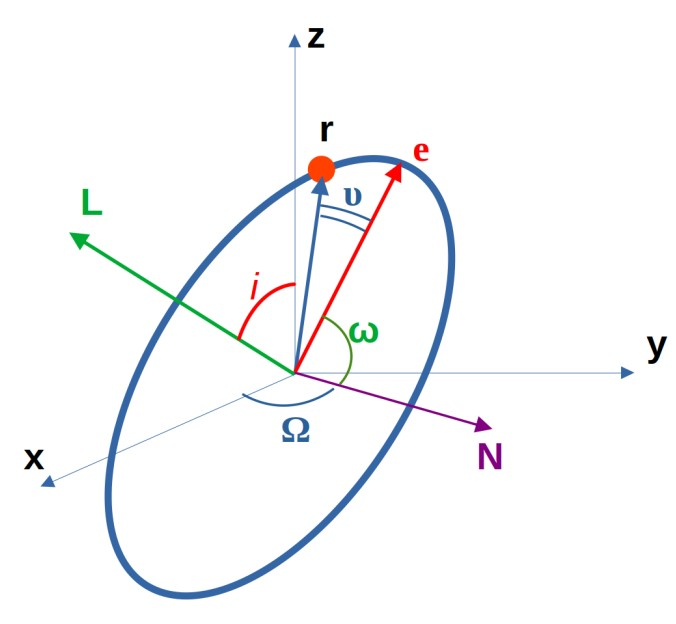
\includegraphics[width=0.6\linewidth]{../images/review/kepler.jpg}
    \captionof{figure}{Кеплеровы элементы орбиты. Центр декартовых координат привязан к центру масс Земли. Ось $Ox$ направлена в точку весеннего равноденствия, 
    ось $Oz$ -- нормаль к плоскости эклиптики, 
    ось $Oy$ дополняет до правой тройки.
    $\mathbf{N}$ лежит на линии пересечения плоскости эклиптики с плоскостью орбиты.
    $\mathbf{L}$ -- момент импульса КО,направлен по нормали к орбитальной плоскости. 
    $\mathbf{e}$ равен по модулю эксцентриситету и направлен на перицентр.}
    \label{fig:kepler}
\end{figure}

Кеплеровы элементы удобны для визуальной интерпретации орбиты (рис. \ref{fig:kepler}).
Первые 3 переменные задают ориентацию орбитальной плоскости в инерциальной системе координат,
эксцентриситет и большая полуось фиксируют форму и размеры эллипса, а истинная аномалия определяет положение КО на орбите.
В качестве последней переменной также могут использоваться эксцентрическая аномалия $E$ и средняя аномалия $M$.
Удобство использования средней аномалии заключается в том, что она меняется со временем равномерно.
Недостаток кеплеровых элементов -- вырожденность при $i = 0$, $i = \pi$ и $e = 0$.
Как следствие, они плохо подходят для интегрирования.

Чтобы избавиться от вырожденности вводится другой набор элементов -- модифицированные равноденственные элементы.
В MEE величина I может принимать два значения:
\[
I = \left\{
\begin{array}{ll}
+1, & \text{если } i < \pi / 2, \\
-1, & \text{если } i \ge \pi / 2
\end{array}
\right.
\]

Также в MEE применяется эксцентрическая долгота $F$ и истинная долгота $L$. 
Они выражаются через кеплеровы элементы следующим образом:
\begin{align*}
    F &= E + \omega + I \Omega \\
    L &= \nu + \omega + I \Omega
\end{align*}

\subsection{Прогноз траектории космического объекта}
Задача прогнозирования движения -- по начальному вектору состояния $X_0$ определить траекторию $X(t)$ объекта.
В основе описания динамики космических аппаратов лежит 2 закон Ньютона, 
поэтому расчет траектории сводится к решению задачи Коши для ОДУ вида:
\begin{equation}
    \begin{cases}
        \dot{X} = f(X, t), \\
        X(t = t_0) = X_0
        \label{eq:prognoz_task}
    \end{cases}
\end{equation}

При расчете траектории применяются несколько существенно разных подходов. 
Первый из них, аналитический, использует основные факторы, определяющие эволюцию орбиты.
Характерной особенностью аналитических вычислений является низкая ресурсоемкость и невысокая точность.
Таким образом, аналитика обладает высокой качественной предсказательной способностью на коротких временных интервалах, 
«схватывая» главные тренды изменения орбиты.

Численные методы, напротив, позволяют учесть произвольное число сложных возмущающих факторов.
Однако прецизионный численный расчет требует значительно больше вычислений. 
Это связано с ресурсоемкостью расчета правой части ОДУ и,
соответственно, с выбором шага интегрирования для обеспечения заданной точности.

Компромиссом являются полуаналитические подходы, 
в которых используется комбинация численных и аналитических расчетов.
Полуаналитические модели учитывают широкий спектр возмущающих воздействий, 
что позволяет эффективно производить вычисления без потери точности.

Далее приведен краткий обзор основных подходов к прогнозу траектории.

\subsubsection{Аналитический прогноз}
Рассмотрим возмущенную задачу двух тел:

\begin{equation}
    \ddot{\mathbf{r}} = - \frac{\mu \mathbf{r}}{r^3} + \mathbf{f},
    \label{eq:analyt_rv}
\end{equation}
где $\mu$ -- гравитационный параметр Земли, $\mathbf{f}$ -- возмущающее ускорение, которое может быть разложено по орбитальной СК на радиальную, тангенциальную и нормальную компоненты:

\begin{equation*}
    \mathbf{f} = R \mathbf{e}_r + T \mathbf{e}_t + N \mathbf{e}_n,
\end{equation*}
\begin{align*}
    \mathbf{e}_r &= \mathbf{r} / |r| \\
    \mathbf{e}_n &= \mathbf{r} \times \mathbf{v} / |\mathbf{r} \times \mathbf{v}| \\
    \mathbf{e}_t &= \mathbf{e_n} \times \mathbf{e_r}
\end{align*}

\begin{figure}[h!]
    \centering
    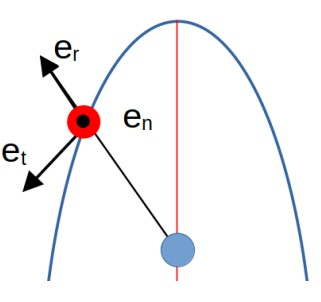
\includegraphics[width=0.4\linewidth]{../images/review/orbital_system.jpg}
    \captionof{figure}{Орбитальная система}
    \label{fig:orbital_system}
\end{figure}

% Byron, p. 485-486
Преобразуем систему ОДУ (\ref{eq:analyt_rv}) для перехода к кеплеровым элементам.
% \begin{align*}
%     & \frac{da}{dt} = \frac{2 a e^2}{h} \sin(\nu) R 
%                     + \frac{2 a^2 h}{\mu r} T \\
%     & \frac{de}{dt} = \frac{h}{\mu} \left[ \sin(\nu) R +
%                      (e + 2 \cos(\nu) + e \cos^2(\nu)) / (1 + e cos \nu) T \right] \\
%     & \frac{di}{dt} = \frac{r}{h} \cos(\omega + \nu) N \\
%     & \frac{d \Omega}{dt} = \frac{r \sin(\omega + \nu) N}{h \sin(i)} \\
%     & \frac{d \omega}{dt} = - \frac{h}{\mu e} \cos(\nu) R 
%                             - \frac{r}{h} \ctg(i) \sin(\omega + \nu) n
%                             + \frac{(h^2 + r \mu) \sin(\nu)}{\mu e h} T \\
%     & \frac{dM}{dt} = n - \frac{1}{na}\left(\frac{2r}{a} - \frac{1 - e^2}{e} \cos(\nu)\right) R
%                         - \frac{1 - e^2}{nae} \left(1 + \frac{r}{p}\right) sin(\nu) T
% \end{align*}
Если возмущающая сила является потенциальной: $\mathbf{f} = \nabla R$, то система примет вид:

\begin{align*}
    & \frac{da}{dt} = \frac{2}{na} \frac{\partial R}{\partial M} \\
    & \frac{de}{dt} = \frac{(1 - e^2)^{1 / 2}}{n a^2 e^2}
                    \left((1 - e^2)^{1 / 2} \frac{\partial R}{\partial M} 
                    - \frac{\partial R}{\partial \omega} \right) \\
    & \frac{di}{dt} = \frac{1}{h \sin(i)} \left(cos(i) \frac{\partial R}{\partial \omega} 
                                                        - \frac{\partial R}{\partial \omega} \right) \\
    & \frac{d \Omega}{dt} = \frac{1}{h \sin(i)} \frac{\partial R}{\partial i} \\
    & \frac{d \omega}{dt} = - \frac{\cos(i)}{h \sin(i)} \frac{\partial R}{\partial i}
                            + \frac{(1 - e^2)^{1 / 2}}{n a^2 e^2} \frac{\partial R}{\partial e} \\
    & \frac{dM}{dt} = n - \frac{1 - e^2}{n a^2 e} \frac{\partial R}{\partial e} 
                        - \frac{2}{na} \frac{\partial R}{\partial a}
\end{align*}
где $n = \sqrt{\frac{\mu}{a^3}}$ -- среднее движение, $h = n a^2 (1 - e^2)^2$.

Для построения аналитического решения воспользуемся возмущающим потенциалом от второй гармоники:
 \begin{equation}
    R = - \frac{\mu J_2}{r} \left( \frac{R_\oplus}{r} \right)^2 
        \frac{3}{2} \left(\sin^2(\phi) - \frac{1}{3}\right),
 \end{equation}
где $\phi$ -- широта точки.

Подставив соотношение $sin(\phi) = sin(i) sin(\omega + \nu)$, получим, что $R$ может быть представлена в виде суммы:

\begin{align*}
    & R = R_s + R_p \\
    & R_s = - \frac{3 \mu J_2}{2 r} \left( \frac{R_\oplus}{r} \right)^2 
            \left( \frac{\sin^2(i)}{2} - \frac{1}{3} \right) \\
    & R_p = \frac{3 \mu J_2}{2 r} \left( \frac{R_\oplus}{r} \right)^2
            \frac{\sin^2(i) \cos(2(\omega + \nu))}{2}
\end{align*}

Видно, что первое слагаемое потенциала вызывает постоянное или так называемое вековое возмущение орбиты. 
Период таких возмущений значительно превышает орбитальный период. 
Короткопериодические возмущения, порождаемые слагаемым $R_p$, не приводят к изменениям орбиты на значительном промежутке времени.

Усреднив $R_s$ по периоду, получим:
\begin{equation*}
    R_{avg} =  - \frac{\mu J_2}{2 a} \left( \frac{R_\oplus}{r} \right)^2 
                \left( \frac{3}{4} \sin^2(i) - \frac{1}{2} \right)
                \left( \frac{1}{(1 - e^2)^{3/2}} \right)
\end{equation*}

Подстановка $R_{avg}$ в ОДУ дает вековые возмущения кеплеровых элементов орбиты

\begin{align*}
    & \dot{a}_{sec} = 0 \\
    & \dot{e}_{sec} = 0 \\
    & \dot{i}_{sec} = 0 \\
    & \dot{\Omega}_{sec} = - \frac{3 n R^{2}_\oplus J_2}{2 p^2} \cos(i) \\
    & \dot{\omega}_{sec} = \frac{3 n R^{2}_\oplus J_2}{4 p^2} (4 - 5 \sin^2(i)) \\
    & \dot{M_0}_{sec} = - \frac{3 n R^{2}_\oplus J_2 \sqrt{1 - e^2}}{4 p ^2}
                            (3 \sin^2(i) - 2)
\end{align*}

Аналогичным образом могут быть выделены короткопериодические возмущения. В частности:

\begin{equation*}
    \delta a = \gamma_3 a \left[ (3z \sin^2(\omega + \nu) - 1) \left(\frac{a}{r}\right)^3
                                    - \frac{3z - 2}{2 \eta^3}  \right],
\end{equation*}
где $\gamma_3 = -J_2 \left(\frac{R_\oplus}{a}\right)^2$, $\eta = \sqrt{1 - e^2}$, $z = \sin^2(i)$.

Так как большая полуось, эксцентриситет и наклонение не испытывают вековых возмущений, 
долгота восходящего узла и аргумент перицентра легко интегрируются аналитически.
\begin{align*}
    & \Omega(t) = \Omega_0 + \Omega_{sec} (t - t_0) \\
    & \omega(t) = \omega_0 + \omega_{sec} (t - t_0) \\
\end{align*}
Для получения выражения для $a$ необходимо провести процедуру усреднения среднего движения
\begin{equation*}
    a = \bar{a} + \delta a \rightarrow  \bar{a} = a_0 - \delta a_0
\end{equation*}
\begin{equation*}
    \bar{n} = \sqrt{\frac{\mu}{\bar{a}^3}}
\end{equation*}

В результате получим:
\begin{equation*}
    M(t) = M_0 + (\bar{n} + \dot{M_0}_{sec}) (t - t_0)
\end{equation*}

Более детальное решение задачи аналитического расчета траектории представлено в серии моделей SGP.
Модели используют данные в формате TLE, предоставляемые американской службой NORAD. 
В TLE содержатся не только средние кеплеровы элементы орбиты, но и первая и вторая производные среднего движения.
Модели движения SGP аналитически учитывают возмущения от сжатия Земли, сопротивления атмосферы, гравитации Луны и Солнца.
Из-за сильного влияния атмосферного торможения ошибка прогноза на низких орбитах составляет порядка 1 километра в день.
Для средних и высоких орбит ошибка значительно меньше -- несколько сотен метров на недельном интервале. 

\subsubsection{Численно-аналитический прогноз}
Стимулом к развитию численно-аналитических методов послужил быстрый рост количества
объектов в околоземном пространстве и необходимость их непрерывного отслеживания и каталогизации.
Для таких задач аналитические методы не удовлетворяют требуемой точности, а численные методы
не подходят в силу высокой ресурсоемкости. Численно-аналитические методы, в свою очередь,
объединяют точность и быстродействие за счет гибкой настройки модели движения.

В основе численно-аналитических моделей лежит разделение возмущений на вековые и короткопериодические.
На начальном этапе происходит усреднение орбитальных элементов, 
чтобы исключить высокочастотные возмущения орбиты. Эта операция позволяет в дальнейшем
интегрировать медленно меняющиеся средние элементы с большим шагом (порядка половины дня).
На заключительном этапе прогноза мгновенные значения элементов орбиты вычисляются аналитически по средним элементам.

Частным случаем численно аналитических методов является модель DSST, разработанная для
системы контроля околоземного пространства Европейского космического агентства (SSA).
Математическая модель DSST опирается на методы усреднения и вариации параметров.

Усредненные уравнения движения для консервативной возмущающей силы:

\begin{equation*}
    \frac{d\bar{c}_i}{dt} = -\sum_{j=1}^{6} \left\{\bar{c}_i, \bar{c}_j \right\} 
                                \frac{\partial \bar{R}}{\partial\bar{c}_j} \qquad i=1 \dots 5
\end{equation*}

При наличии неконсервативной силы правая часть дополнительно усредняется по витку:

\begin{equation*}
    \frac{d\bar{c}_i}{dt} = \frac{1}{2 \pi} \int_{0}^{2 \pi} \frac{\partial\bar{c}_i}{\partial\dot{\mathbf{r}}} 
                        \cdot \mathbf{Q} d\lambda \qquad i=1 \dots 5
\end{equation*}

Выражение для быстроменяющейся средней долготы:

\begin{equation*}
    \frac{d \bar{\lambda}}{dt} = \frac{d\bar{c}_6}{dt} = 
        \bar{n} -\sum_{j=1}^{6} \left\{\bar{c}_6, \bar{c}_j \right\} 
                                \frac{\partial \bar{R}}{\partial\bar{c}_j}
                +\frac{1}{2 \pi} \int_{0}^{2 \pi} \frac{\partial\bar{c}_6}{\partial\dot{\mathbf{r}}} 
                        \cdot \mathbf{Q} d\lambda
\end{equation*}

Переход к мгновенным элементам:

\begin{equation*}
    c_i = \bar{c}_i + \sum_{j=1}^{N} e^j \eta_{i, j}\left(\bar{a}, \bar{\lambda}\right) \qquad i = 1 \dots 6
\end{equation*}

В последних уравнениях были введены следующие обозначения:
\begin{align*}
    \bar{c}_{i=1 \dots 6} &: \text{средние равноденственные элементы} \left[\bar{h}, \bar{k}, \bar{k}, \bar{p}, \bar{q}, \bar{\lambda}\right] \\
    \bar{R} &: \text{усредненный возмущающий потенциал для консервативной силы} \\
    \mathbf{Q} &: \text{неконсервативная сила} \\
    \bar{n} &: \text{усредненное среднее движение} \\
    \left\{\bar{c}_i, \bar{c}_j \right\} &: \text{скобки Пуассона} \\
    \eta_{i, j} &: 2\pi \text{-периодические функции}
\end{align*}

Точность прогноза по модели DSST отличается для разных классов орбит.
Среднеквадратичное отклонение при сравнении с численным расчетом на 7 суток составляет от 10 метров для НОО до 20 метров для ГСО.
Для высокоэллиптических орбит среднеквадратичная ошибка может достигать 75 метров.

\subsubsection{Численный прогноз}

В ходе численного прогноза производится интегрирование системы \eqref{eq:prognoz_task}.
Для этого на каждом шаге требуется вычислять значение правой части $f(X, t)$. 
В задачах небесной механики правая часть определяется суммарной силой, действующей на КА.
Среди сил, влияющих на баллистическое движение КА основными являются:
\begin{itemize}
    \item Притяжение Земли
    \item Сопротивление атмосферы
    \item Солнечное давление
    \item Притяжение планет Солнечной системы
    \item Давление света, отраженного от поверхности Земли (эффект альбедо)
\end{itemize}

Среди этих сил на НОО основной вклад вносят притяжение Земли и сопротивление атмосферы.
С ростом высоты плотность атмосферы экспоненциально падает и на высотах порядка 800 километров
сила атмосферного сопротивления становится сопоставима с силой солнечного давления.

Помимо сил, имеющих природное происхождение, на КА могут действовать силы техногенного характера, 
в частности, сила тяги двигателей КА.

В специфических случаях высокоточного прогноза траектории необходимо учитывать
силы, вызванные тепловым излучением аппарата вследствие неравномерного нагрева (эффект Ярковского), 
а также силу, создаваемую антенной-излучателем.

В дальнейшем основные из перечисленных сил будут рассмотрены подробнее.

\paragraph{Притяжение Земли.}

Отличие гравитационного потенциала Земли от сферического обсусловлено 
сложной формой геоида и динамикой его изменения. Результирующий потенциал представим в виде разложения
в сферических координатах ($r$, $\phi$, $\lambda$):

\begin{equation*}
    U = \frac{\mu}{r} + 
    \frac{\mu}{r} \sum_{n=1}^{\infty} \left(\frac{R}{r}\right)^n 
    \sum_{m=0}^{n} P_{nm}(\sin\phi) \left[ S_nm \sin(m \lambda) + C_nm \cos(m \lambda) \right]
\end{equation*}
$P_{nm}$ -- присоединенные полиномы Лежандра, $R$ -- экваториальный радиус модели, 
$C_{nm}$ и $S_{nm}$ -- коэффициенты модели.

Ускорение от силы притяжения рассчитывается из градиента гравитационного потенциала:

\begin{equation*}
    \ddot{\mathbf{r}}_{\text{грав}} = -\nabla U
\end{equation*}

В настоящее время существует множество различных моделей потенциала Земли.
Для баллистических расчетов в околоземном пространстве широко используется статическая модель EGM2008.
Максимальный порядок модели составляет 2159, с дополнительными коэффициентами вплоть до 2190 степени.
Для повышения динамической точности к модели могут применяться поправки, вызванные
твердотельными и океаническими приливами. Данные для построения модели были получены из
анализа относительного движения аппаратов миссии GRACE, спутниковой альтиметрии и 
территориальных гравиметрических измерений. 

\paragraph{Сопротивление атмосферы}

Сила аэродинамического сопротивления, действующего на КА, может быть рассчитана по формуле:

\begin{equation*}
    \mathbf{F}_{\text{атм}} = - \frac{C \rho |v| S}{2} \mathbf{v},
\end{equation*}
где $C$ -- коэффициент аэродинамического сопротивления, $\rho$ -- атмосферная плотность,
$\mathbf{v}$ -- скорость движения аппарата относительно атмосферы, S -- площадь поперечного сечения.

Основные вычислительные затраты при расчете силы сопротивления приходятся на модель атмосферы.
Атмосферная плотность зависит от многих параметров: координат, солнечной активности,
геомагнитной активности, календарного сезона и времени суток.

В результате солнечной активности верхние слои атмосферы облучаются ультрафиолетом,
что вызывает увеличение плотности. Атмосфера не прозрачна для ультрафиолета,
поэтому измерить исходное УФ излучение с Земли невозможно. Было установлено, что
излучение с длиной волны 10.7 сантиметров (2800 МГц), порождается тем же слоем Солнца, что и
ультрафиолет. Это позволило косвенно измерять силу УФ излучения через индекс
солнечной актвиности $F_{10.7}$, характеризующий спектральную мощность излучения на единицу поверхности. Единица $F_{10.7}$ соответствует
$10^{-22} \frac{\text{Вт}}{\text{м}^2 \text{Гц}}$. 
Измерения $F_{10.7}$ производятся в канадской обсерватории. 
Величина индекса связана с 11-летним циклом солнечной активности. 
В пике $F_{10.7}$ может достигать значений 300 -- 350, в то время как в периоды спада
солнечной активности его величина составляет порядка 70 -- 100 единиц. 
Во многих моделях применяется не только мгновенное, но и усредненное за 81 день значение индекса.
Данный интервал усреднения охватывает 3 периода вращения Солнца. 
Каждый цикл солнечной активности уникален, 
поэтому точное предсказание индекса на длительный срок невозможно.

Следующим фактором, влияющим на плотность атмосферы, является магнитная активность.
Солнечный ветер, то есть поток ионизированных частиц, 
вызывает возмущения магнитного поля Земли и нагревает верхние атмосферные слои.
Для описания геомагнитной активности используется планетарный квази-логарифмический индекс $K_p$.
Его значения варьируются от 0 для низкой активности до 9 для магнитных штормов c дробным шагом 1/3. 
$K_p$ сопоставлен линейный индекс $A_p$, пропорицональный амплитуде возмущений магнитного поля.
Единица $A_p$ соответствует $10^{-9}$ Тл. $A_p$ лежит в диапазоне от 0 до 400, но в среднем величина индекса составляет 10 -- 20 с редкими всплесками.
Индексы геомагнитной активности формируются каждые 3 часа на основе измерений 12 обсерваторий.
Динамика $K_p$ и $A_p$, как и $F_{10.7}$, зависит от фазы солнечного цикла.
Пик возмущений магнитного поля приходится на фазу спада солнечной активности.

Учет положения Солнца также существенен при расчете атмосферной плотности.
Освещенные участки атмосферы нагреваются, поэтому плотность в этих областях существенно
больше, чем в затененных.

Большинство современных моделей полуэмпирические. В их основе лежит комбинация не только
физических законов, но и экспериментальных данных. 
Классические представители полуэмпирических моделей -- ГОСТ 25645.166--2004 и NRLMSISE-00.

Модель ГОСТ 25645.166--2004 создана на основе данных о торможении спутников в атмосфере.
Она позволяет вычислять атмосферную плотность для высот от 120 до 1500 километров с учетом
изменений плотности ночной атмосферы в течение 11-летнего солнечного цикла, суточных изменений,
сезонных изменений, колебаний солнечной активности и изменений в магнитном поле.
Данная модель -- стандарт для отечественных баллистических расчетов.

При разработке модели NRLMSISE-00 были использованы данные акселерометров на спутниках,
радарные измерения температуры экзосферы и измерения концентрации ионов кислорода.
Помимо колебаний солнечной и магнитной активности в модели
учтены годовые, полугодовые, суточные, полусуточные и третьсуточные изменения плотности.
Структура модели позволяет рассчитывать плотность, гибко настраивая набор учитываемых параметров.
Несмотря на то, что выпущена более новая версия -- NRLMSIS-21, 
модель NRLMSISE-00 остается наиболее востребованной в силу баланса точности и ресурсоемкости.

Среди перспективных направлений совершенствования методов вычисления атмосферной плотности 
можно выделить расчет поправок к существующим моделям с помощью анализа торможения спутников
в атмосфере. Искомые поправки можно получить из процедуры минимизации в ходе
восстановления орбиты для большого числа КА с известными
аэродинамическими параметрами.

\paragraph{Притяжение третьих тел.}
Для расчета притяжения третьих тел необходимо принять во внимание относительное движение
Земли, КА и третьего тела:

\begin{equation*}
    \ddot{\mathbf{r}}_{\text{3-тело}} = \mu_3 \left( \frac{\mathbf{r}_{\text{sat3}}}{r^3_{sat3}}
                                    - \frac{\mathbf{r}_{\text{3}}}{r^3_{3}} \right),
\end{equation*}
где $\mu_3$ -- гравитационный параметр третьего тела,
 $\mathbf{r}_{\text{sat3}}$ -- вектор КА--тело, 
 $\mathbf{r}_{3}$ -- вектор Земля--тело. 

Заметим, что в формуле учтена только центральная гармоника гравитационного потенциала третьего тела.
Такое приближение полностью оправдано при расчете околоземных орбит.
При прогнозе межпланетных траекторий притяжение планет солнечной системы может быть 
более точно представлено через разложение потенциала.

Эфемериды планет в формате DE405 предоставляются лабораторией JPL в виде наборов полиномов Чебышева для
каждого временного интервала. Средняя точность эфемерид составляет 0.01''.

\paragraph{Солнечное давление.}
Как и атмосферное сопротивление, сила солнечного давления не консервативна. Выражение для силы следует из формулы давления
электромагнитного излучения:

\begin{equation*}
    \mathbf{F}_{\text{сол}} = -\frac{W}{c} C_R S_{\text{сол}} \frac{\mathbf{r}_{\text{сол}}}{r_{\text{сол}}},
\end{equation*}
где $W$ -- энергетический поток, $c$ -- скорость света,
$C_R$ -- отражательная способность поверхности КО,
$S$ -- освещенная площадь КО,
$\mathbf{r}_{\text{сол}}$ -- радиус вектор Солнца относительно Земли.

Энергия солнечного излучения убывает обратно пропорционально квадрату расстояния, следовательно
энергетический поток может быть найден как:

\begin{equation*}
    W = TSI \frac{AU^2}{r^2_{\text{сол}}},
\end{equation*}
где TSI -- энергетический поток на расстоянии одной астрономической единицы AU.
Данные TSI формируются на базе спутниковых измерений.

Давление излучения Солнца воздействует на аппарат только в освещенных участках орбиты,
поэтому для вычисления силы солнечного давления необходимо знать границы теневой области.

Наиболее простая модель тени цилиндрическая (\ref{fig:cylindrical_shadow}). Ее недостаток заключается в резком переходе
свет--тень и соответствующих нежелательных разрывах при численном интегрировании.
Коническая модель тени (\ref{fig:conic_shadow}) позволяет учесть полутеневые участки и избавиться от разрывов.
В работе !!!! предложен аналитический алгоритм определения границ полутеневых областей в конической модели
и методика коррекции шага численного интегрирования в участках перехода свет--тень. 
Среди аналитических подходов широко применяется метод, основанный на геометрическом
расчете площади перекрытия Солнца и Земли (\ref{fig:area_shadow}). Минусом данного подхода является необходимость
вычислять перекрытие на каждом шаге. 
Существует также динамическая модель SOLAARS CF, включающая рефракцию атмосферы и
сплюснутость Земли, но
ее применение ограничено высокой ресурсоемкостью.

\begin{figure}[ht]
  % Левый блок: 2 вертикальные картинки
  \begin{minipage}[c]{0.68\textwidth}
    \centering
    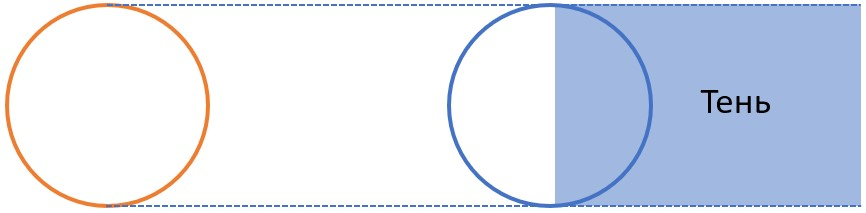
\includegraphics[width=\linewidth, height=6cm, keepaspectratio, valign=c]{review/cylindrical_shadow.jpg}
    \captionof{figure}{Цилиндрическая модель тени}
    \label{fig:cylindrical_shadow}
    
    \vspace{0.5cm} % Отступ между картинками
    
    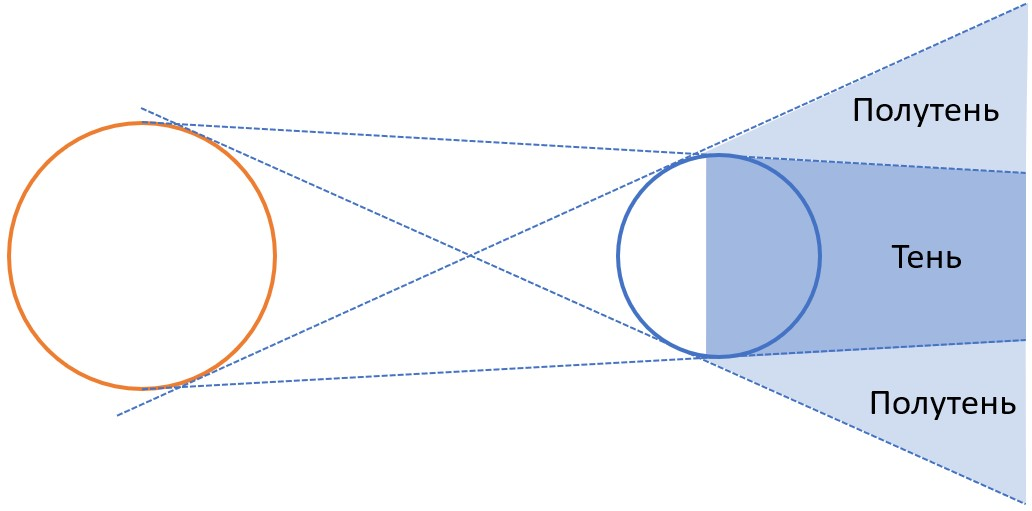
\includegraphics[width=\linewidth, height=6cm, keepaspectratio, valign=c]{review/conic_shadow.jpg}
    \captionof{figure}{Коническая модель тени}
    \label{fig:conic_shadow}
  \end{minipage}
  \hfill
  % Правый блок: 1 картинка по центру
  \begin{minipage}[c]{0.3\textwidth}
    \centering
    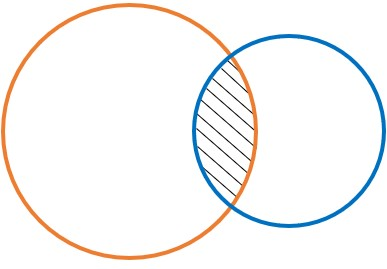
\includegraphics[width=\linewidth, height=6.5cm, keepaspectratio, valign=c]{review/area_shadow.jpg}
    \captionof{figure}{Модель тени с перекрытием}
    \label{fig:area_shadow}
  \end{minipage}

  \label{fig:combined}
\end{figure}

\paragraph{Альбедо.}
Эффект альбедо связан с попаданием на спутник света, отраженного от Земли, и теплового излучения планеты.
Значение отражательной способности сильно зависит от рода поверхности, на которую падает излучение.
Карта альбедо (\ref{fig:albedo_map}) и тепловая карта для Земли создаются на основе спутниковых измерений, а сила давления излучения,
действующая на спутник, рассчитывается для каждой части поверхности Земли отдельно и затем суммируется.

\begin{figure}[h!]
    \centering
    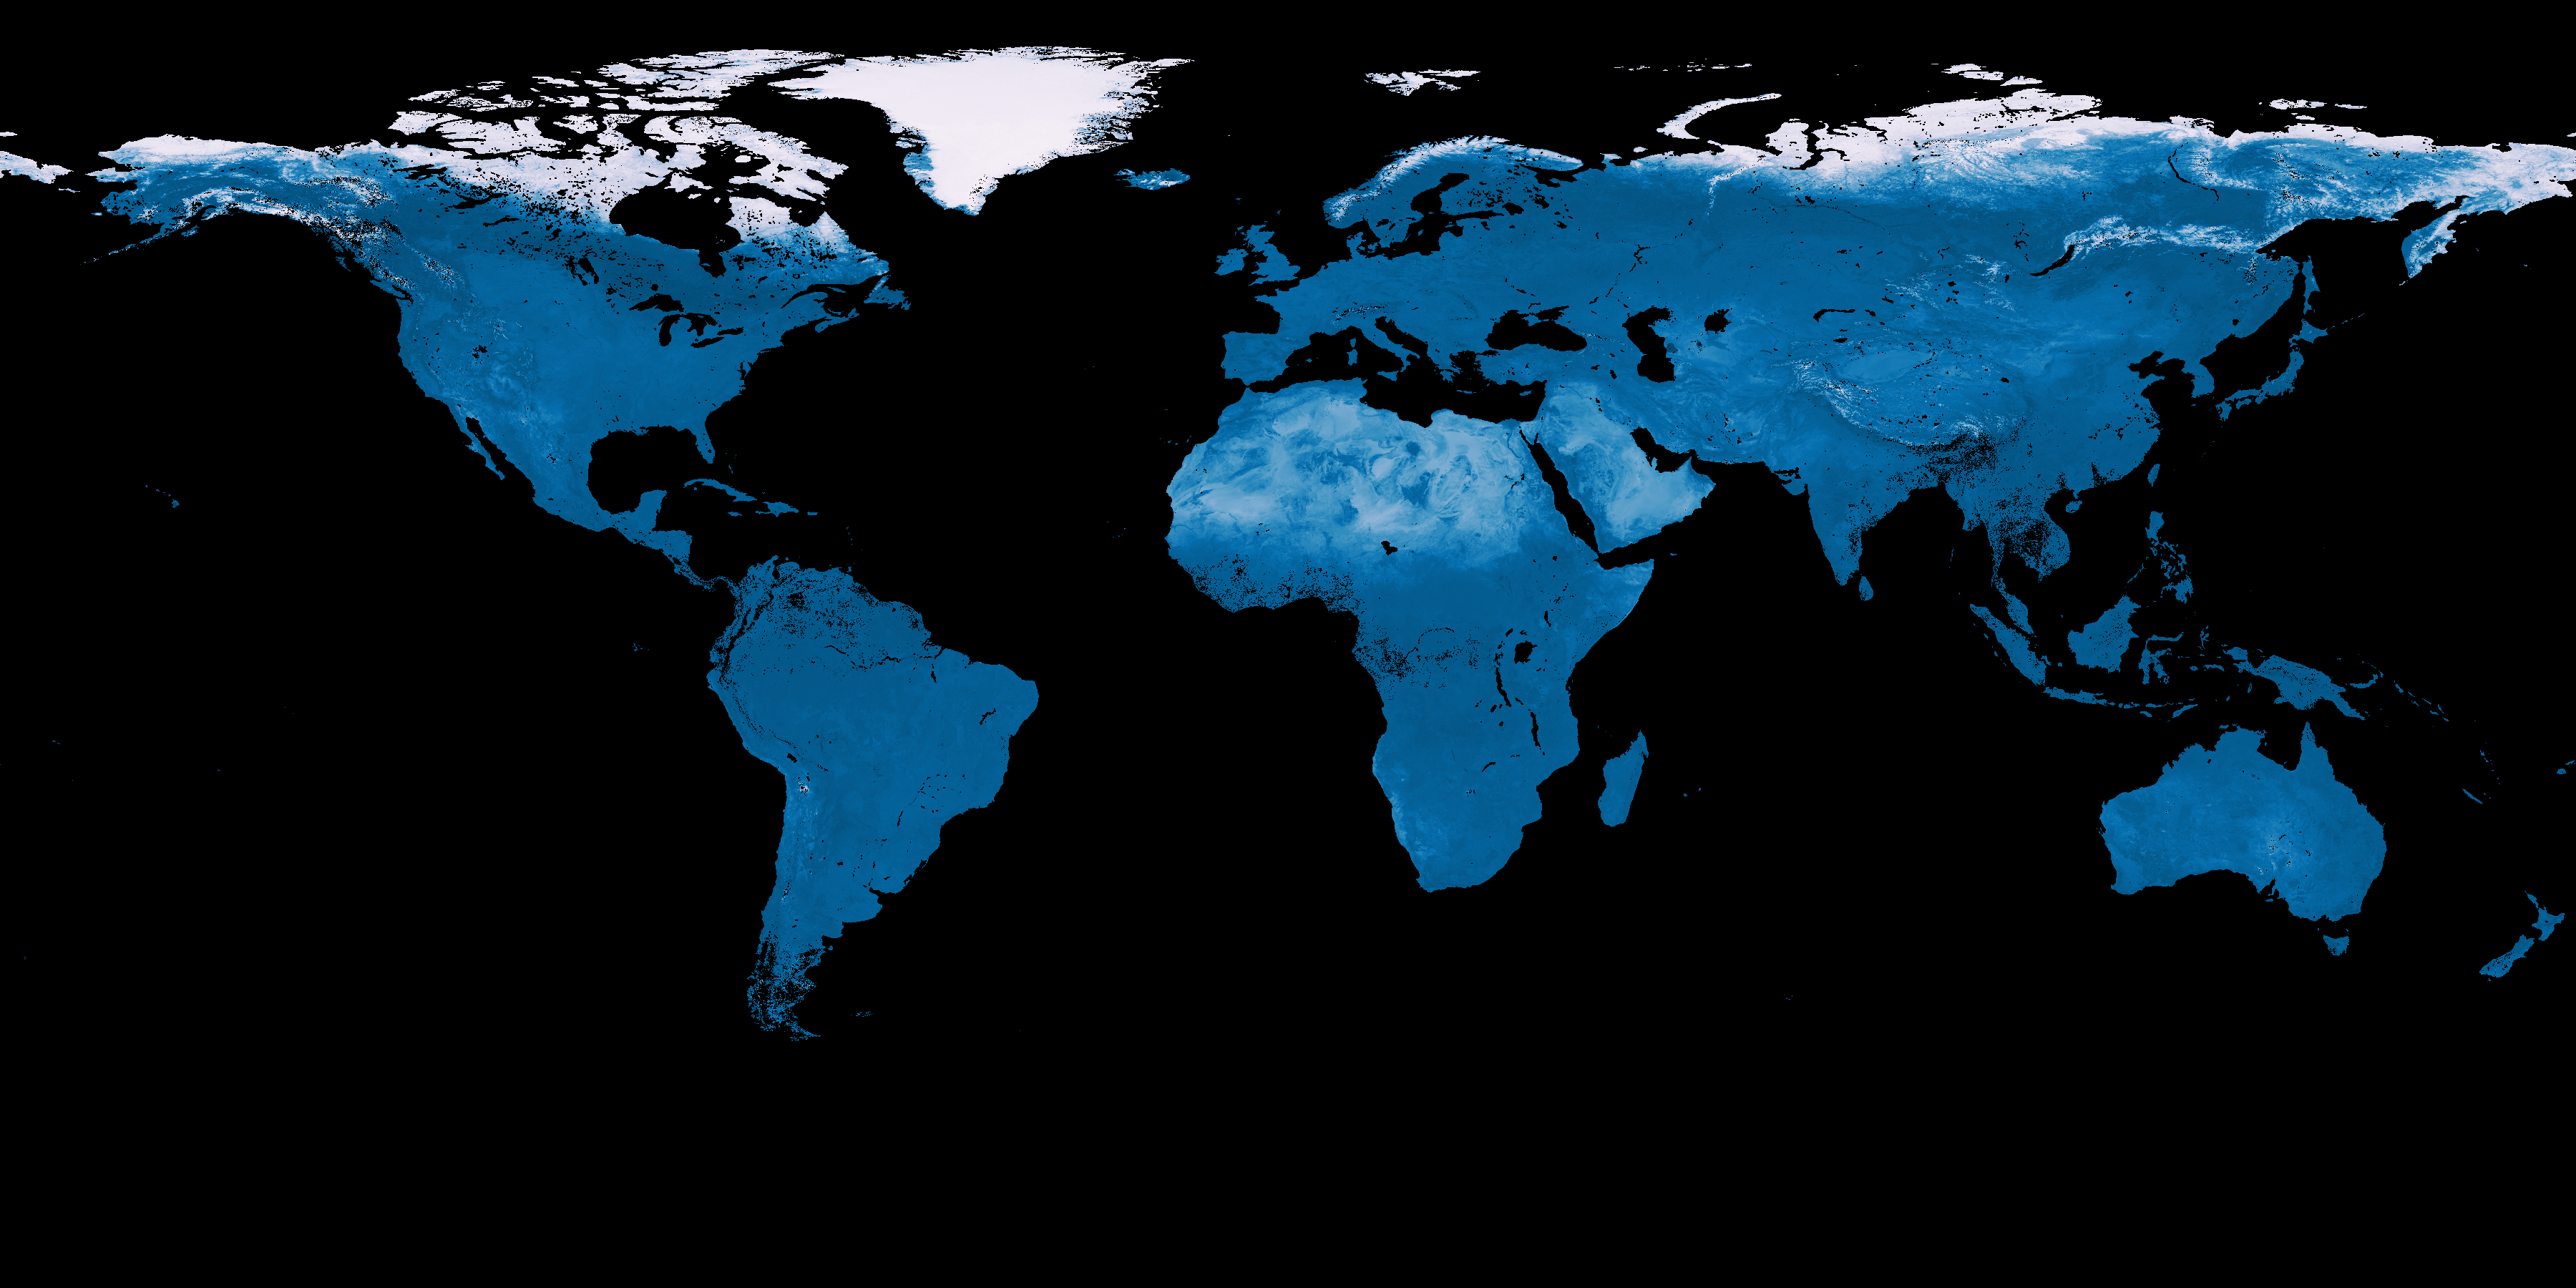
\includegraphics[width=\linewidth]{review/albedo_map.jpg}
    \captionof{figure}{Карта альбедо, май 2025 г. Светлые участки
    соответствуют областям с высокой отражательной способностью}
    \label{fig:albedo_map}
\end{figure}

% Модель измерений
\subsection{Типы измерений}

Для уточнения орбиты требуются измерения параметров, связанных с положением и движением КО.
Конкретный набор измеряемых параметров зависит от типа используемых наблюдательных средств.
Рассмотрим несколько классических наборов измеряемых величин.

\subsubsection{Односторонние измерения дальности}
Расстояние между спутником и станцией наблюдения является одним из наиболее часто измеряемых параметров.
Такая модель измерений получила широкое распространение во многом благодаря глобальным навигационным спутниковым системам.
Каждый спутник ГНСС оснащен антенной, которая излучает электромагнитные волны на нескольких частотах.
Сигнал каждого спутника модулируется особым образом, чтобы приемник мог определить момент времени $T_{T}$ излучения волны по шкале времени спутника
и соответствующие этому моменту координаты излучателя. Момент приема сигнала $T_{R}$ фиксируется по часам приемника.

Зная разницу между временем отправки и приема сигнала, а также используя свойство прямолинейности распространения света, можно 
рассчитать величину, называемую псевдодальностью:
\begin{equation*}
    \rho = (T_{R} - T_{T}) c,
\end{equation*}
где $c$ -- скорость света.

Псевдодальность не совпадает с геометрической в силу несогласованности часов излучателя и приемника, 
особенностей распространения сигнала в атмосфере и относительного движения излучателя и приемника.

Учет этих факторов необходим при формировании расчетного аналога измерения:

\begin{equation*}
    \tilde{\rho} = |\vec{r}_{T} - \vec{r}_{R}| 
                    + c \left( \delta t_{T} - \delta t_{R} \right)
                    + \delta \rho_{tropo} + \delta \rho_{ion} + \epsilon,
\end{equation*}
где помимо геометрической дальности $|\vec{r}_{T} - \vec{r}_{R}|$ присутствуют слагаемые,
связанные с поправкой часов спутника $\delta t_{T}$ и станции $\delta t_{R}$, тропосферная $\delta \rho_{tropo}$ и ионосферная $\delta \rho_{ion}$ задержки.
Благодаря измерениям на нескольких частотах ионосферная задержка может быть с высокой точностью исключена.
В $\epsilon$ включаются остаточные ошибки, связанные с неучитываемыми нелинейными эффектами.

Для повышения точности позиционирования и уменьшения разброса результатов
в ходе решения навигационной задачи могут обрабатываться не только псевдодальности,
но и фазовые измерения сигнала. 
В этом случае точность позиционирования с использованием ГНСС может достигать 10 сантиметров.

\subsubsection{Двусторонние измерения дальности}
В ходе двустороннего измерения дальности фиксируется время, за которое излученный сигнал
достигает цели, отражается и возвращается в точку испускания. 
Вариантом такой измерительной системы является лазерная дальнометрия (SLR).
В отличии от односторонних измерений дальности в лазерной дальнометрии излучатель и приемник
находятся в одном месте и подключены к одним часам, что избавляет от необходимости уточнения поправок шкал времени.
При этом атмосферные поправки все еще требуются. 
В качестве измерений усредняется расстояние, пройденное сигналом в прямом и обратном направлениях:

\begin{equation*}
    \rho_{avg} = \frac{1}{2} \left[ 
        \left(T_{R} - T_{T}\right) c + \delta \rho_{atm} + \epsilon \right]
\end{equation*}

Современные станции SLR используют лазеры с длиной волны 532 нм, что соответствует оптическому диапазону.
С этим связан недостаток лазерной дальнометрии -- зависимость от погодных условий.

В качестве примера применения SLR рассмотрим серию аппаратов LAGEOS (LAser GEOdynamics Satellite).
Аппараты LAGEOS-I и LAGEOS-II были запущены на среднюю околоземную орбиту в 1976 и 1992 годах соответственно.
Цель миссии -- изучение геодинамики, в частности, определение формы земной поверхности и уточнение параметров вращения Земли. 
Каждый аппарат имеет шарообразную форму и оснащен набором уголковых отражателей, необходимых
для точного отражения лазерного сигнала.

Позиционирование спутников выполняется на основе измерений наблюдательных пунктов Международной службы лазерной дальнометрии.
Ошибки лазерных измерений составляют менее 1 сантиметра, что позволяет восстанавливать орбиту аппаратов с точностью до нескольких сантиметров.

\subsubsection{Оптические измерения}


\subsubsection{Лазерные}

% Обработка измерений
\subsection{Обработка измерений}
Существует два качественно разных подхода к обработке поступающих измерений
для уточнения параметров орбиты.
Первый подход базируется на совместной обработке измерительной информации. 
Представителем данного подхода является метод наименьших квадратов (МНК).
На начальных этапах освоения космоса именно этот метод использовался
для восстановления орбит КА. 
С увеличением числа объектов в околоземном пространстве рос и объем ресурсов, 
требующийся для процедуры уточнения орбит.
Это привело к появлению менее трудоемких алгоритмов, основанных 
на линеаризации уравнений динамики системы и рекуррентной обработке измерений. Примером таких
алгоритмов служит фильтр Калмана и его модификации.

\subsubsection{Метод наименьших квадратов}
В методе наименьших квадратов параметры орбиты $\mathbf{x}$ итеративно 
подбираются таким образом,
чтобы минимизировать взвешенную сумму квадратов невязок измерений 
$\{\mathbf{z}^O_k (t_k, \mathbf{x})\}_{k=1}^N$ 
и их расчетных аналогов $\{\mathbf{z}_k^C (t_k, \mathbf{x})\}_{k=1}^N$:

\begin{equation}
    S(\mathbf{x}) = \sum_{k=1}^{N} (\mathbf{z}^O_k - \mathbf{z}^C_k)^T W_k 
    (\mathbf{z}^O_k - \mathbf{z}^C_k) \rightarrow min,
\end{equation}
где $N$ -- число измерений, $W_k$ -- весовая симметричная матрица, $t_k$ -- момент измерения, а
расчетные аналоги строятся из прогноза движения КА на моменты измерений.

Задачу оптимизации можно переписать в виде:

\begin{equation*}
    S(\mathbf{x}) = (\mathbf{z}^O - \mathbf{z}^C)^T W (\mathbf{z}^O - \mathbf{z}^C) \rightarrow min,
\end{equation*}
где $\mathbf{z}^C = (z_1^C, \dots, z_N^C)$, 
$\mathbf{z}^O = (z_1^O, \dots, z_N^O)$, $W = diag(W_1, \dots, W_N)$.

Рассмотрим поиск минимума функционала методом Гаусса-Ньютона, также
известным как метод дифференциальной коррекции. В данном алгоритме 
используется предположение о близости начального приближения к оптимальному, что позволяет
провести линеаризацию расчетного аналога измерений:

\begin{equation*}
    \mathbf{z}^C = \mathbf{z}^N (\mathbf{x}) +  
    \frac{\partial \mathbf{z}^N (\mathbf{x})}{\partial \mathbf{x}} \Delta \mathbf{x} = 
    \mathbf{z}^N + A \Delta \mathbf{x},
\end{equation*}
где $\mathbf{z}^N$ -- номинальный вектор измерений, соответствующий состоянию системы на текущей итерации,
 $A (\mathbf{x}) = \frac{\partial z^N (\mathbf{x})}{\partial \mathbf{x}}$ -- матрица Якоби,
 $\Delta \mathbf{x}$ -- параметр линеаризации.

На каждой итерации необходимо найти такой шаг $\Delta \mathbf{x}$, который обеспечивал бы
минимум невязки. Из необходимого условия экстремума:

\begin{equation*}
    \nabla S(\mathbf{x}) = - 2 A^T (\mathbf{x}) W (\mathbf{z}^O (\mathbf{x}) - \mathbf{z}^C) = 0
\end{equation*}

\begin{equation*}
    A^T W (\mathbf{z}^O - \mathbf{z}^C) 
    = A^T W (\mathbf{z}^O - \mathbf{z}^N) - A^T W A \Delta \mathbf{x} = 0
\end{equation*}

Обозначая $\mathbf{z}^O - \mathbf{z}^N = \mathbf{b}$, получим выражение для шага:
\begin{equation}
    \Delta \mathbf{x} = (A^T W A)^{-1} A^T W \mathbf{b}
\end{equation}

Таким образом, имея начальное приближение $\mathbf{x}_{0}$, можно построить итеративную процедуру:
\begin{equation}
    \mathbf{x}_{i + 1} = \mathbf{x}_{i} + \Delta \mathbf{x}
\end{equation}

Выбор начального приближения может быть осуществлен с помощью методов начального
определения орбиты, таких как методы Гаусса, Гудинга и Double-R.

Критерий останова -- малое изменение среднеквадратичного отклонения по сравнению с предыдущей итерацией.

Матрица Якоби $A_k$ измерения $\mathbf{z}_k$ представима в виде произведения:

\begin{equation*}
    A_k(\mathbf{x}) = \frac{\partial \mathbf{z}_k (\mathbf{\tilde{x}})}{\partial \mathbf{\tilde{x}}}
    \frac{\partial \mathbf{\tilde{x}} (\mathbf{x}, t_k)}{\partial \mathbf{x}} = H_k \Phi_k,
\end{equation*}
где $\mathbf{\tilde{x}}$ -- прогноз состояния системы на момент времени $t_k$, 
а матрица $H_k$ может быть рассчитана аналитически.

Матрица изохронных производных $\Phi_k$ вычисляется 
из интегрирования уравнения в вариациях до момента времени $t_k$:
\begin{equation}
    \begin{cases}
        \dot{\Phi} = \frac{\partial \mathbf{f}}{\partial \mathbf{x}} \Phi, \\
        \Phi \big|_{t = t_0} = E,
        \label{eq:prognoz_phi}
    \end{cases}
\end{equation}
где $\mathbf{f}$ -- правая часть системы (\ref{eq:prognoz_task}), $E$ -- единичная матрица.

МНК требует точную, а, следовательно, вычислительно-затратную модель эволюции системы, но
взамен дает высокую точность определения орбиты и согласующих параметров (например,
отношения площади КА к массе).

\subsubsection{Фильтр Калмана}
Фильтр Калмана -- рекурсивный фильтр, использующий модель движения системы и
измерения датчиков (в том числе и с зашумлением) для оценки вектора состояния системы.

Каждая итерация фильтра включает прогноз на основе текущего состояния и уточнение прогноза
с учетом измерения. Исходно фильтр Калмана создавался для линейных систем. Задачи
баллистики существенно нелинейны, поэтому для их решения были разработаны 
расширенный и сигма-точечный фильтр Калмана. 

Рассмотрим динамическую систему со следующей моделью:

\begin{equation*}
    \begin{cases}
        \dot{\mathbf{x}}(t) = \mathbf{f}(\mathbf{x}(t), t) + \mathbf{w}(t), \\
        \mathbf{x}(t_0) \sim \mathcal{N}\left(\bar{\mathbf{x}}_0, P_0 \right),
    \end{cases}
\end{equation*}
где $\mathbf{w}(t)$ -- вектор шума модели с матрицей ковариации Q.

С помощью датчика можно получать измерения параметров системы $\mathbf{z}_k$ в моменты времени $t_k$:

\begin{equation*}
    \mathbf{z}_k = \mathbf{h} (\mathbf{x}(t_k), t_k) + \mathbf{v}_k,
\end{equation*}
где $\mathbf{h} (\mathbf{x}, t)$ -- функция чувствительности системы, $\mathbf{v}_k$ --
нормально распределенный шум измерения с нулевым математическим ожиданием и матрицей
ковариации $R_k$. Предполагается, что шумы $w$ и $v$ не коррелируют.

Задача фильтрации заключается в рекурсивном вычислении оптимальной оценки состояния
по набору измерений $\{\mathbf{z}_k\}_{k=1}^N$. 

\paragraph{Расширенный фильтр Калмана} \mbox{} \\

В основе расширенного фильтра Калмана линеаризация в окрестности отфильтрованной
оценки состояния системы на каждом шаге. Прогноз вектора состояния до коррекции $\mathbf{x}_{k|k-1}$
производится по формуле:

\begin{equation*}
    \mathbf{x}_{k|k-1} = \mathbf{x}_{k-1|k-1} 
    + \Delta t \cdot \mathbf{f} (\mathbf{x}_{k-1|k-1}, t_{k-1}),
\end{equation*}
где $\mathbf{x}_{k-1|k-1}$ -- вектор состояния на предыдущем шаге.

Затем вычисляется прогноз матрицы ковариации, и оба прогноза корректируются по 
следующему измерению.

Учитывая процедуру линеаризации, использование высокоточной модели движения в
фильтре Калмана нецелесообразно. Упрощенная модель динамики и рекуррентная обработка
измерений приводит к низкой ресурсоемкости процесса фильтрации, что особенно важно
для бортовых вычислительных систем. Однако недостаток линеаризации выражается в значительном
росте ошибок на больших промежутках времени.

\paragraph{Сигма-точечный фильтр Калмана} \mbox{} \\

Вместо линеаризации эта модификация фильтра Калмана использует сигма-точки,
расположенные в окрестности текущей оценки состояния. Эти точки "пробуют" возможные
варианты развития системы, а потом объединяются для уточненного прогноза:

\begin{equation*}
    \mathbf{x}_{k|k-1} = \sum_{i = 0}^{2n} W_i^{(m)} \mathbf{x}^{*}_{i, k-1|k-1},
\end{equation*}
где $W_i^{(m)}$ -- веса сигма-точек, $\mathbf{x}^{*}_{i, k-1|k-1}$ -- вектора состояния в сигма-точках.

% Проблематика
\subsection{Проблематика}
На сегодняшний день на околоземных орбитах находится большее число космических объектов.
Среди них есть не только активные аппараты, но и космический мусор, образовавшийся
в результате фрагментации корпусов ракет и спутников.
Растущая загруженность околоземной среды требует развития эффективных средств контроля 
космического пространства, в частности, для уточнения орбит КО.
В основе восстановления орбиты лежит задача прогнозирования движения.
Для построения траектории необходимо вычислять силы, действующие на космический объект.

\subsubsection{Оценка быстродействия}
Краткий обзор вычислительных сложностей приведен в таблице \ref{tab:force_perf}.

\begin{table}[h!]
\renewcommand{\arraystretch}{1.5}
\begin{tabular}{|cc|c|l}
\cline{1-3}
\multicolumn{2}{|c|}{Сила}                & Время расчёта, усл. ед. &  \\ \cline{1-3}
\multicolumn{1}{|c|}{\multirow{3}{*}{Гравитационное притяжения}} &
  16*16 гармоник &
  1 &
   \\ \cline{2-3}
\multicolumn{1}{|c|}{} & 64*64 гармоник   & 12.3                    &  \\ \cline{2-3}
\multicolumn{1}{|c|}{} &
  \begin{tabular}[c]{@{}c@{}}64*64 гармоник (ускорение)\end{tabular} &
  1.3 &
   \\ \cline{1-3}
\multicolumn{1}{|c|}{\multirow{3}{*}{Сопротивление атмосферы}} &
  ГОСТ Р 25645.166-2004 &
  2.2 &
   \\ \cline{2-3}
\multicolumn{1}{|c|}{} & NRLMSISE-00      & 14                      &  \\ \cline{2-3}
\multicolumn{1}{|c|}{} & NRLMSIS 2.1      & 86                      &  \\ \cline{1-3}
\multicolumn{1}{|c|}{\multirow{2}{*}{Солнечное давление}} &
  точечного источника &
  0.06 &
   \\ \cline{2-3}
\multicolumn{1}{|c|}{} & непрерывной тени & 0.1                     &  \\ \cline{1-3}
\end{tabular}%
\caption{Сравнение времени вычисления некоторых сил, действующих на КО}
\label{tab:force_perf}
\end{table}

Сила гравитационного притяжения вычислялась с использованием модели EGM2008 для
разного числа гармоник. За единицу принята трудоемкость подсчета с учетом 16*16 гармоник.

Среди рассмотренных сил на низкой орбите основной вклад вносят гравитационное притяжение Земли 
и сопротивление атмосферы.
В классических подходах наиболее ресурсоемким этапом является вычисление силы гравитационного 
притяжения Земли. Ресурсоемкость вычисления данной силы с ростом числа гармоник растет квадратичною.
Соответствующие затраты для 64*64 гармоник составили 12 условных единиц.
Однако использование интерполяционного подхода \cite{kuznetsov2023} позволяет существенно 
снизить ресурсоемкость расчета гравитационной силы. С учетом интерполяции время
расчета силы притяжения равно времени, затрачиваемому на прямой расчет гравитационной силы
с учетом 16 гармоник потенциала. 

Таким образом, именно расчет силы 
сопротивления атмосферы становится ключевым с точки зрения ресурсоемкости программы.
Вычисление аэродинамического сопротивления атмосферы связано 
с определением ее плотности.
Для повышения эффективности программного комплекса требуется ускорение расчета атмосферной плотности.
Алгоритм, позволяющий осуществить это, рассмотрен в следующем разделе.

\subsubsection{Высокоточное восстановление орбиты}
Точность восстановления орбиты КО зависит от динамической модели и измерений.
Для систем, использующих измерения высокой точности, например лазерную дальнометрию,
качества прямого моделирования сил начинает не хватать на интервалах по времени
больше дня. Это связано с тем, что моделирование
любой силы, действующей на КО, содержит определенную ошибку. Особенно сильно эта ошибка
проявляется при расчете давления солнечного излучения и эффекта Альбедо. Величина этих
сил определяется ориентацией КО. Если объект обладает сложной конструктивной геометрией,
то вычислить площадь поверхности, на которую падает излучение, и модуль силы затруднено. 

Для того чтобы преодолеть это, вводится дополнительная параметризация модели сил,
реализация которой будет представлена далее.

\newpage
    \section{Ускорение расчета плотности атмосферы}
\label{sec:Chapter2} \index{Chapter2}

В настоящей работе исследуется возможность ускорения расчета плотности атмосферы c
использованием интерполяционных подходов.

Существует несколько хорошо известных алгоритмов многомерной интерполяции. Полилинейная и
поликубическая интерполяция, а также интерполяция до ближайшего характеризуются низкой
вычислительной сложностью, но малой точностью. 
Компромиссом является интерполяция на узлах Чебышева--Лиссажу \cite{dencker2017}, обеспечивающая
быструю многомерную интерполяцию с сохранением высокой точности. 
Именно этот алгоритм был выбран для интерполяции модели атмосферы.

\subsection{Обзор алгоритма интерполяции}
Первый этап создания интерполянта на узлах Чебышева--Лиссажу заключается в построении 
прямоугольной сетки в $\mathbb{R}^d$. В частном случае это сетка в
околоземном пространстве в координатах $(r, \phi, \lambda, t)$.

Затем для ячейки сетки вычисляется набор точек, являющихся обобщением
узлов Чебышева--Гаусса--Лобатто на $d$--мерное пространство:

\begin{equation*}
    \begin{cases*}
        \mathbf{z_{\mathbf{i}}^{\mathbf{(\mathbf{n})}}} = (z_{i_1}^{n_1}, \dots, z_{i_d}^{n_d}) \\
        z_i^{n} = \cos (i \pi / n)
    \end{cases*}
\end{equation*}

Наборы $\mathbf{i} \in \mathbb{N}^d$ состоят либо лишь из четных, либо только из нечетных чисел, при этом каждое
число не превышает соответствующее число из $\mathbf{n} \in \mathbb{N}^d$, 
состоящего из взаимно простых чисел и определяющего конфигурацию интерполянта.

Эти узлы лежат в точках самопересечения кривых Лиссажу:

\begin{equation*}
    \mathbf{l} = \left(\cos \left( \frac{\pi * p[\mathbf{n}]}{n_1} \right), 
                \dots,\cos \left( \frac{\pi * p[\mathbf{n}]}{n_d} \right) \right),
\end{equation*}
где $p[\mathbf{n}] = \prod_{j=1}^{d} n_j$.

Визуализация узлов и кривых Лиссажу для трехмерного пространства представлена на рис. \ref{fig:chebLis}.

\begin{figure}[h!]
    \centering
    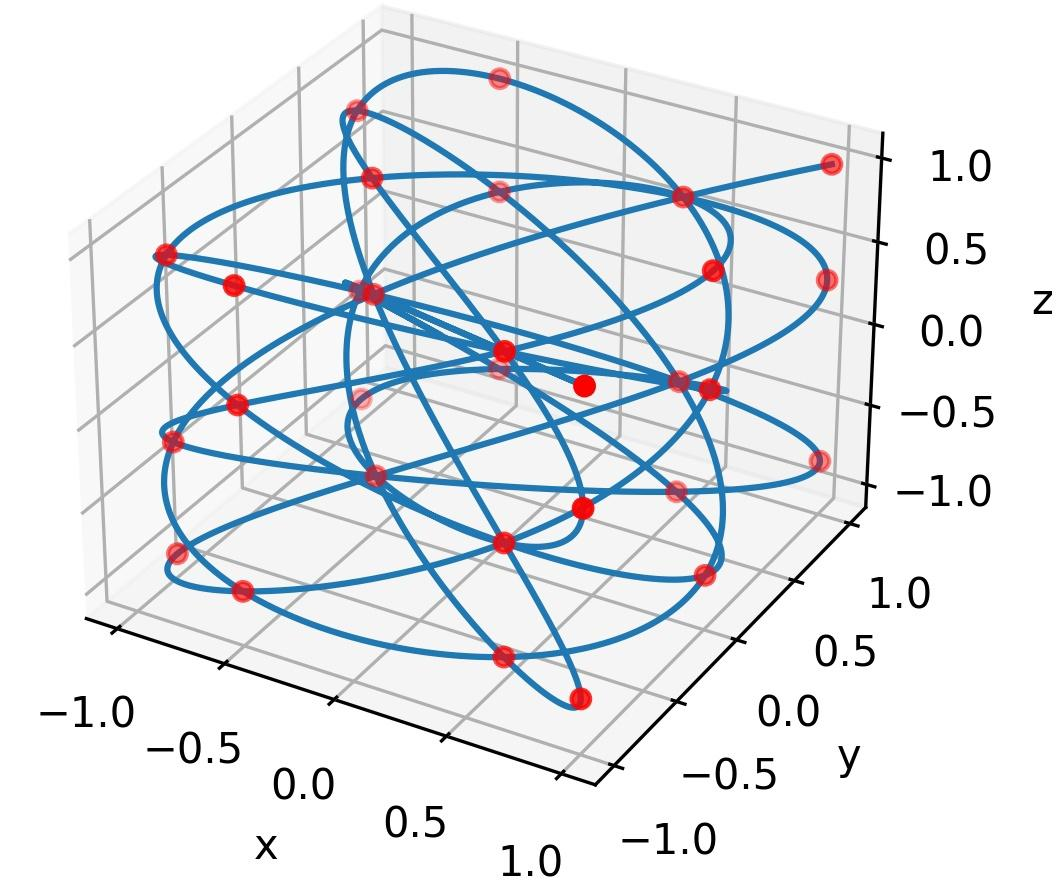
\includegraphics[width=0.5\linewidth]{../images/solution/chebLis.png}
    \captionof{figure}{Узлы Чебышева--Лиссажу в единичном кубе}
    \label{fig:chebLis}
\end{figure}

Теперь необходимо найти d-мерный полином, удовлетворяющий условию интерполяции.

Полиномы Чебышева имеют следующий вид:
\begin{equation*}
    T_{\gamma} (x) = \cos (\gamma \arccos (x))
\end{equation*}

В узлах Чебышева--Лиссажу:
\begin{equation*}
    T_{\gamma} (z^n_i) = \cos \left(\gamma \arccos \left(\cos \left(\frac{i \pi}{n}\right) \right)\right)
     = \cos(\gamma \frac{i \pi}{n}) \equiv \chi_{\gamma}^n (i)
\end{equation*}

Определим d-мерные полиномы Чебышева как:
\begin{equation*}
    T_{\mathbf{\gamma}} = T_{\gamma_1} \cdot \dots \cdot T_{\gamma_d},
\end{equation*}
где $\mathbf{\gamma} \in \mathbb{N}^d_0$.
Они составляют ортогональный базис в d-мерном пространстве полиномов. Аналогично,
\begin{equation*}
    \chi_{\mathbf{\gamma}}^{\mathbf{n}} (\mathbf{i}) = \prod_{j=1}^{d} \cos(\gamma_j \frac{i_j \pi}{n_j})
\end{equation*}
В свою очередь $\chi_{\mathbf{\gamma}}^{\mathbf{n}} (\mathbf{i})$ составляют базис в пространстве
функций $L^2$.

Этот факт дает возможность разложить, функцию $h$, заданную на узлах, по данному базису, чтобы
получить коэффициенты интерполяции:
\begin{equation*}
    \begin{cases*}
        h \approx \sum_{\mathbf{\gamma}} c_{\mathbf{\gamma}} (h) \chi_{\mathbf{\gamma}}^{\mathbf{n}} \\
        c_{\mathbf{\gamma}} (h) = \frac{1}{|| \chi_{\mathbf{\gamma}}^{\mathbf{n}} ||^2}
        \left(h, \chi_{\mathbf{\gamma}}^{\mathbf{n}}\right)
    \end{cases*}
\end{equation*}

Вид базисных функций позволяет последовательно
применить дискретное косинус преобразование к каждой размерности для эффективного подсчета
коэффициентов. 

В результате функция может быть аппроксимирована линейной комбинацией произведений
многочленов Чебышева:
\begin{equation*}
    h \approx \sum_{\mathbf{\gamma}} c_{\gamma} T_\gamma
\end{equation*}

В частном случае интерполяции 4-мерной функции плотности атмосферы
результат интерполяции представим в виде:
\begin{equation*}
    \ln(\rho) \approx \sum_{i,j,k,l}^{n_1, n_2, n_3, n_4} 
    c_{i,j,k,l} T_i(r) T_j(\phi) T_k (\lambda) T_l (t),
\end{equation*}
где $T_\alpha$ -- полином Чебышева степени $\alpha$.

Интерполяция логарифма объяснятся тем фактом, что зависимость убывания
атмосферной плотности с высотой примерно экспоненциальная.

Точность интерполяции определяется количеством ячеек, на которое было разбито пространство
и максимальной степенью полиномов по размерности для каждой ячейки. При построении
интерполянта расчет ячеек независим, что дает возможность вычислять коэффициенты в ячейках
параллельно на нескольких потоках.

Скорость интерполяции зависит от конфигурации интерполянта. Чем больше степени полиномов в
каждой ячейке, тем сильнее увеличивается время подсчета.

\subsection{Тестирование интерполяции}

Проведено тестирование точности различных конфигураций интерполянтов для модели NRLMSISE-00.
Диапазон интерполяции по расстоянию был выбран от 350 до 800 километров, интервал по времени
составил одни сутки. В ходе тестов была использована космическая погода за 11 января 2014 года.
Этот год соответствует высокой солнечной активности, что позволяет протестировать качество
интерполяции в сложных условиях.

Сетка для проверки работы алгоритма состояла из более 1 миллиона точек, равномерно
распределенных по области интерполяции. Для каждого интерполянта измерялась максимальная
ошибка на тестовой сетке, размер и величина ускорения по сравнению с прямым расчетом плотности.

Полный перебор по возможным конфигурациям и количеству ячеек интерполянтов сложен
из-за большого количества вариантов, времени, затрачиваемого на построение каждого интерполянта и
занимаемой памяти. Поэтому поиск подходящих параметров проводился поэтапно.

Учитывая близкую к линейной зависимость логарифма плотности от высоты, для этой координаты
была выбрана наименьшая степень полинома -- 2. В рассмотрении остались наборы 
(2, 3, 5, 7), (2, 3, 7, 5), (2, 5, 3, 7), (2, 5, 7, 3), (2, 7, 3, 5),
(2, 7, 5, 3). Интерполянты для полиномов более
высоких порядков не строились из-за снижения производительности таких конфигураций и
существенного повышения затрат памяти для хранения коэффициентов.

Для каждого набора было зафиксировано количество ячеек по высоте -- 65. Количество ячеек
по широте, долготе и времени варьировалось от 5 до 50. Эмпирически определялось
количество ячеек для достижения точности при заданном разбиении по высоте. Далее
для интерполянта с максимальным числом ячеек по широте, долготе и времени варьировалось
количество ячеек по высоте и определялась точность, достижимая с такими параметрами.

На рисунках \ref{fig:atmo:2357} -- \ref{fig:atmo:2753} представлены зависимости относительной ошибки от количества ячеек по
конкретной координате интерполянта. Для времени фиксировалось
максимальное количество ячеек по остальным координатам. Для долготы и широты
фиксировалось наиболее плотное разбиение по широте и долготе соответственно, а диапазон
соответствует вариации количества ячеек по времени.

\begin{figure}[h!]
    \centering
    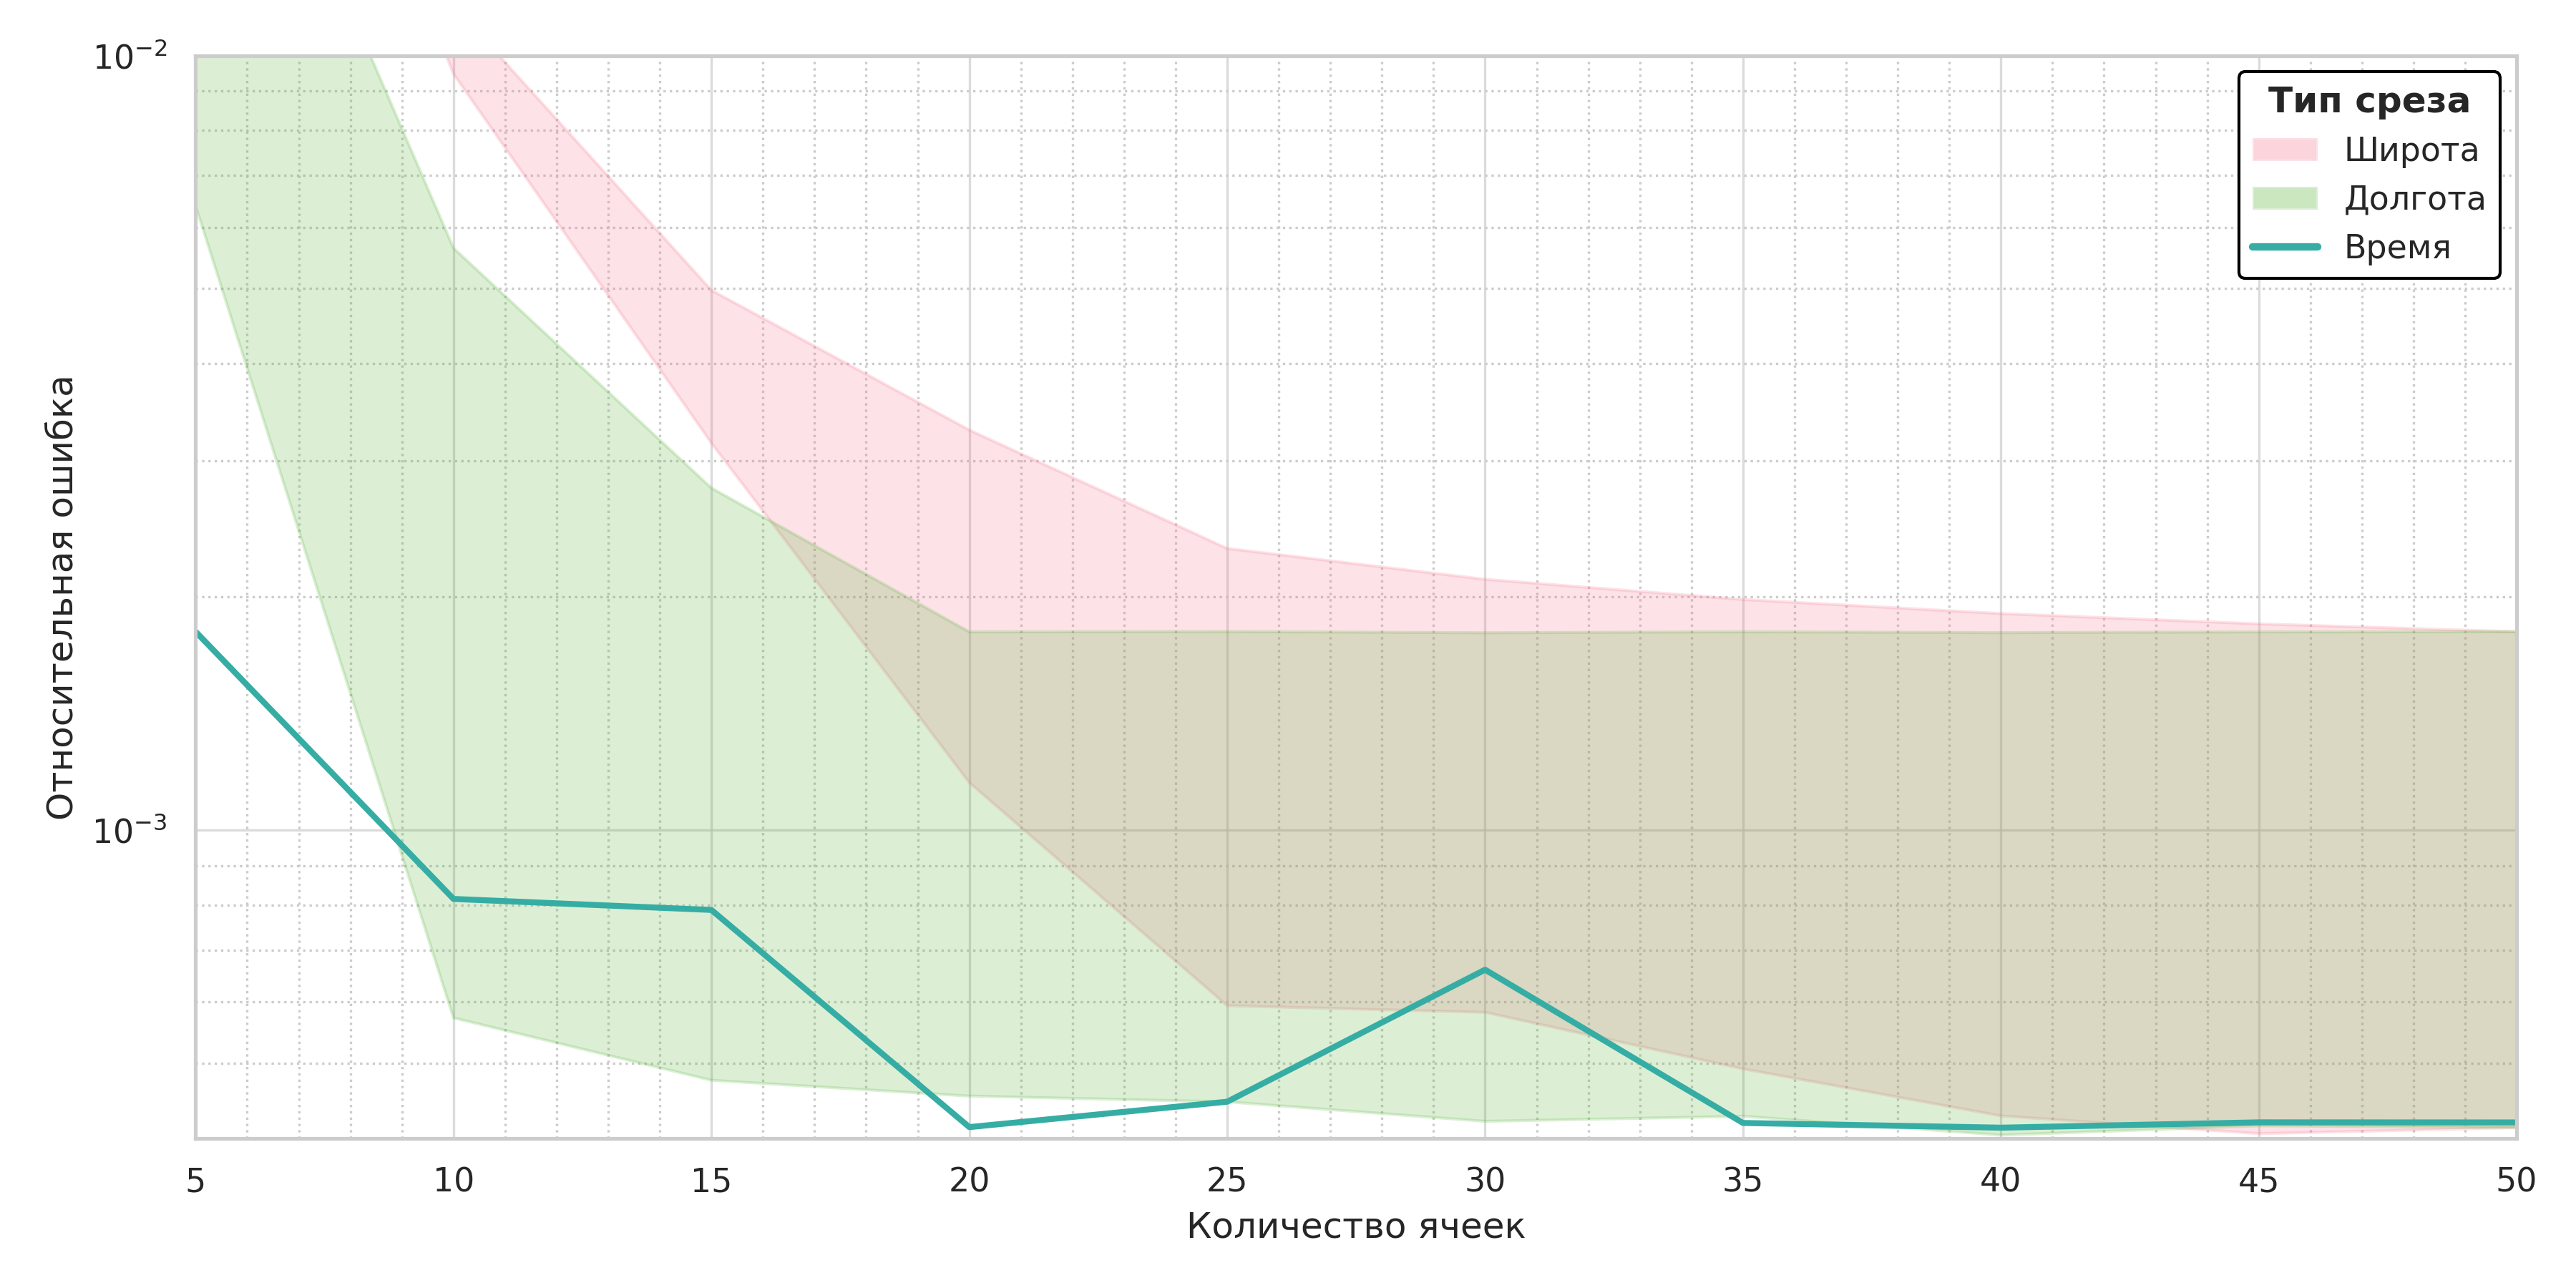
\includegraphics[width=\linewidth]{../images/solution/atmo/2357.png}
    \captionof{figure}{Зависимость ошибки от количества ячеек интерполянта для конфигурации (2, 3, 5, 7)}
    \label{fig:atmo:2357}
 \end{figure}

 \begin{figure}[h!]
    \centering
    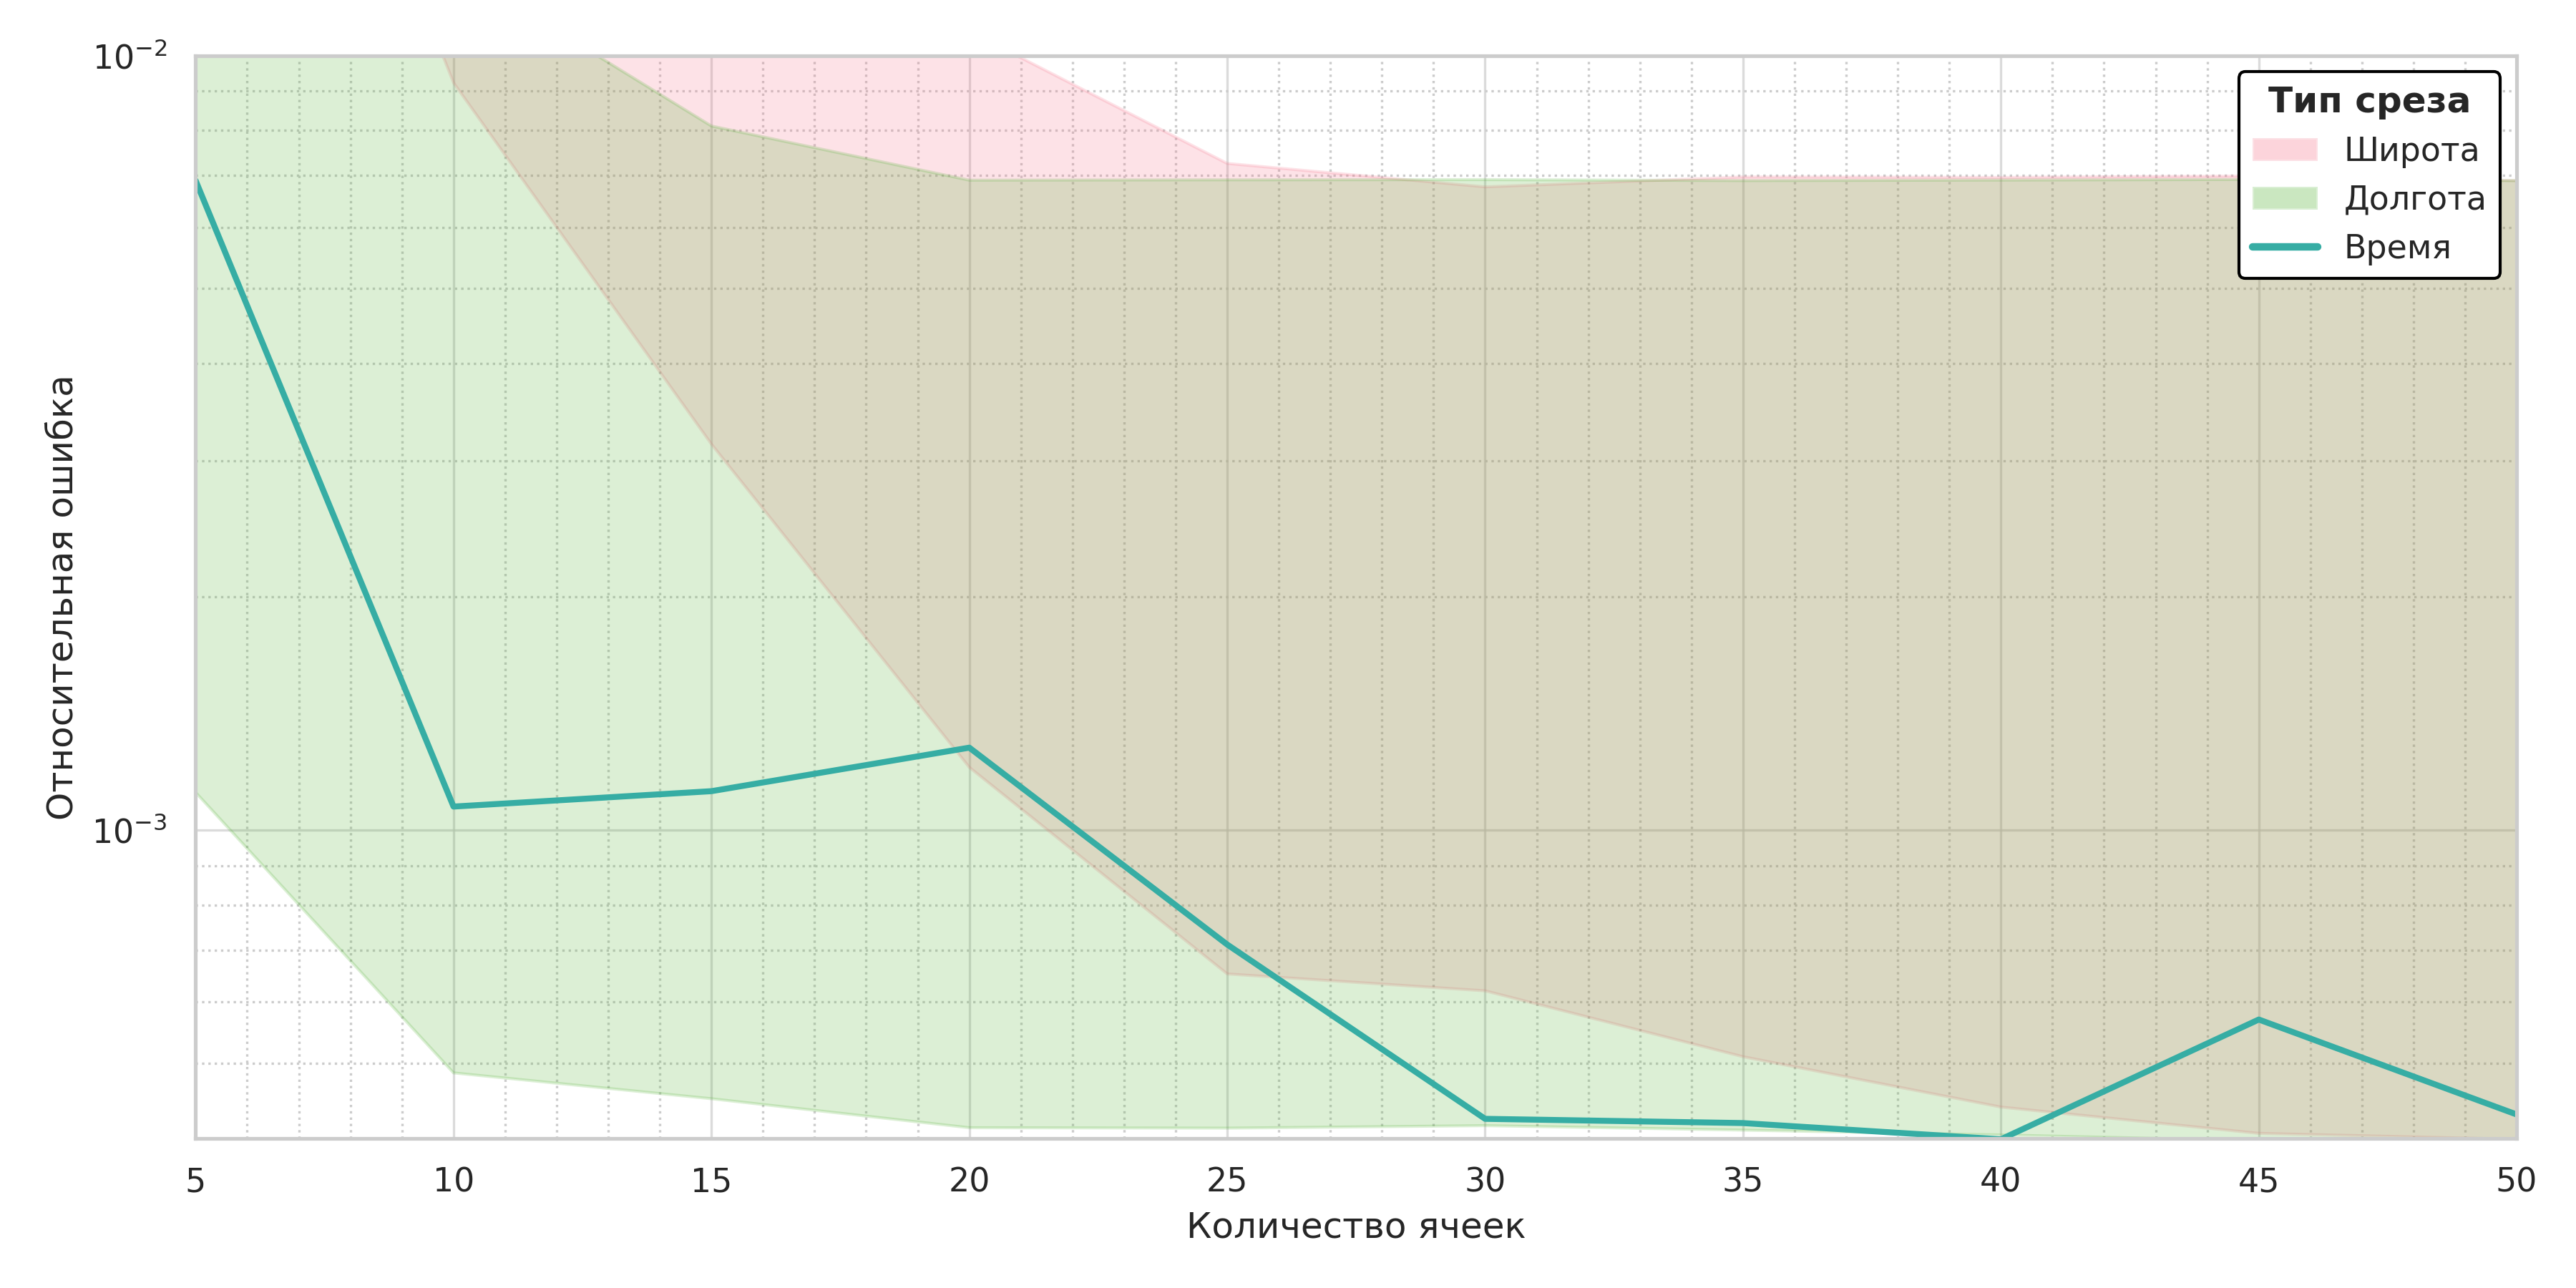
\includegraphics[width=\linewidth]{../images/solution/atmo/2375.png}
    \captionof{figure}{Зависимость ошибки от количества ячеек интерполянта для конфигурации (2, 3, 7, 5)}
    \label{fig:atmo:2375}
 \end{figure}

 \begin{figure}[h!]
    \centering
    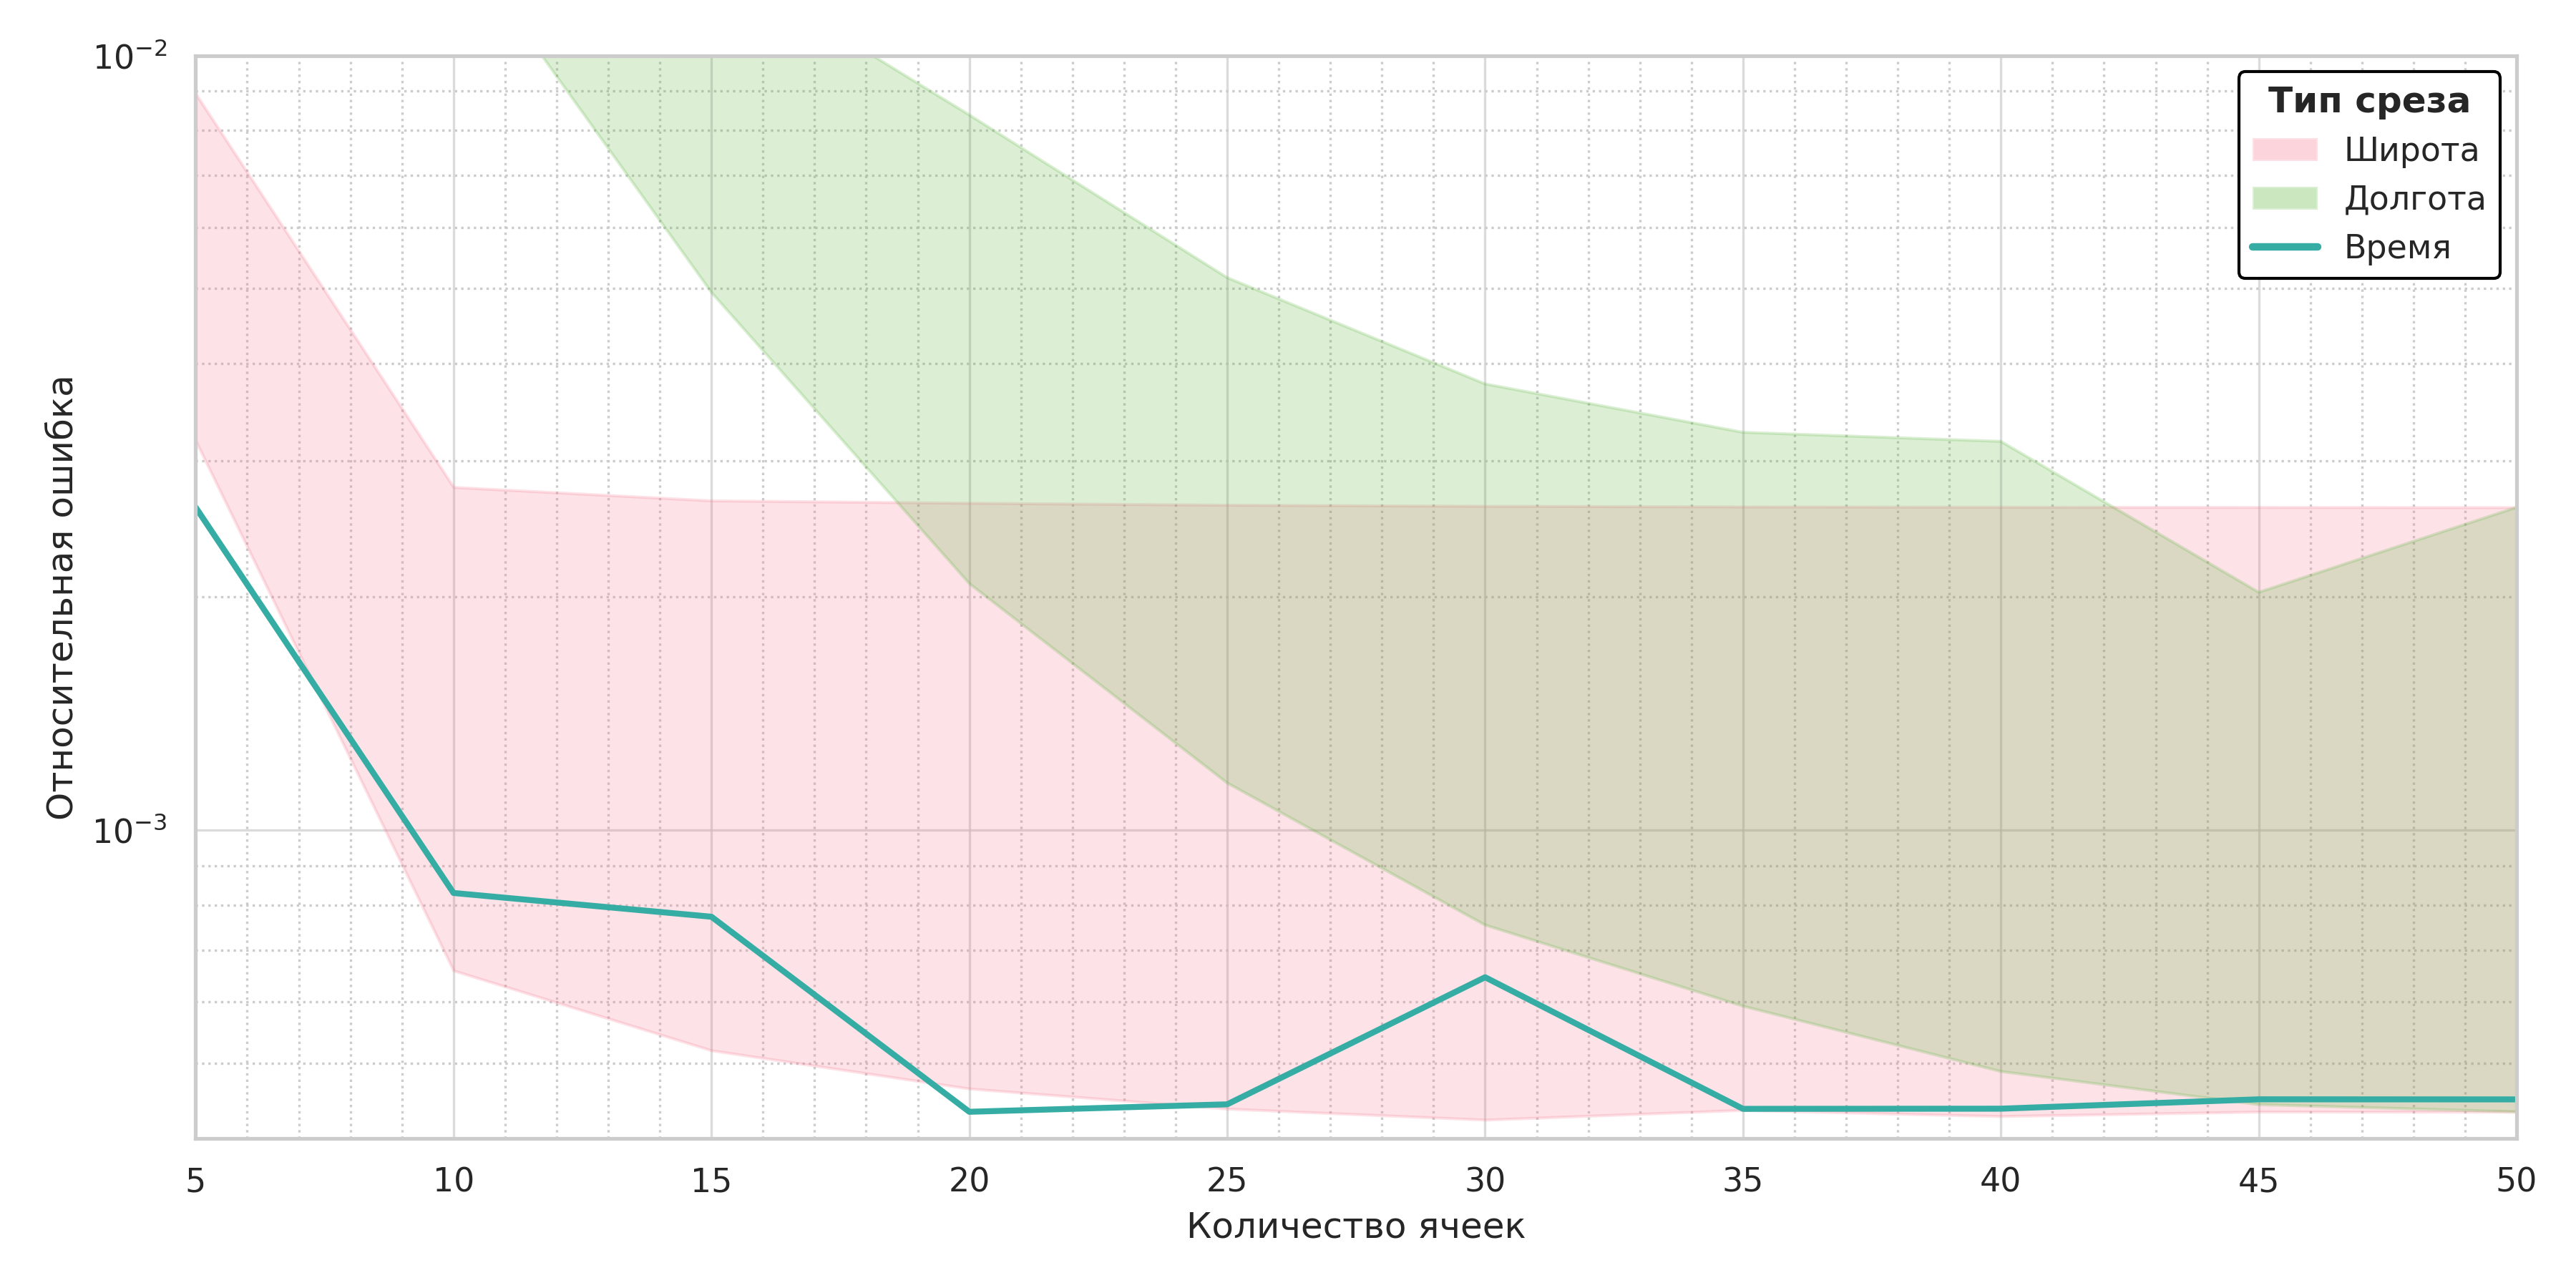
\includegraphics[width=\linewidth]{../images/solution/atmo/2537.png}
    \captionof{figure}{Зависимость ошибки от количества ячеек интерполянта для конфигурации (2, 5, 3, 7)}
    \label{fig:atmo:2537}
 \end{figure}

 \begin{figure}[h!]
    \centering
    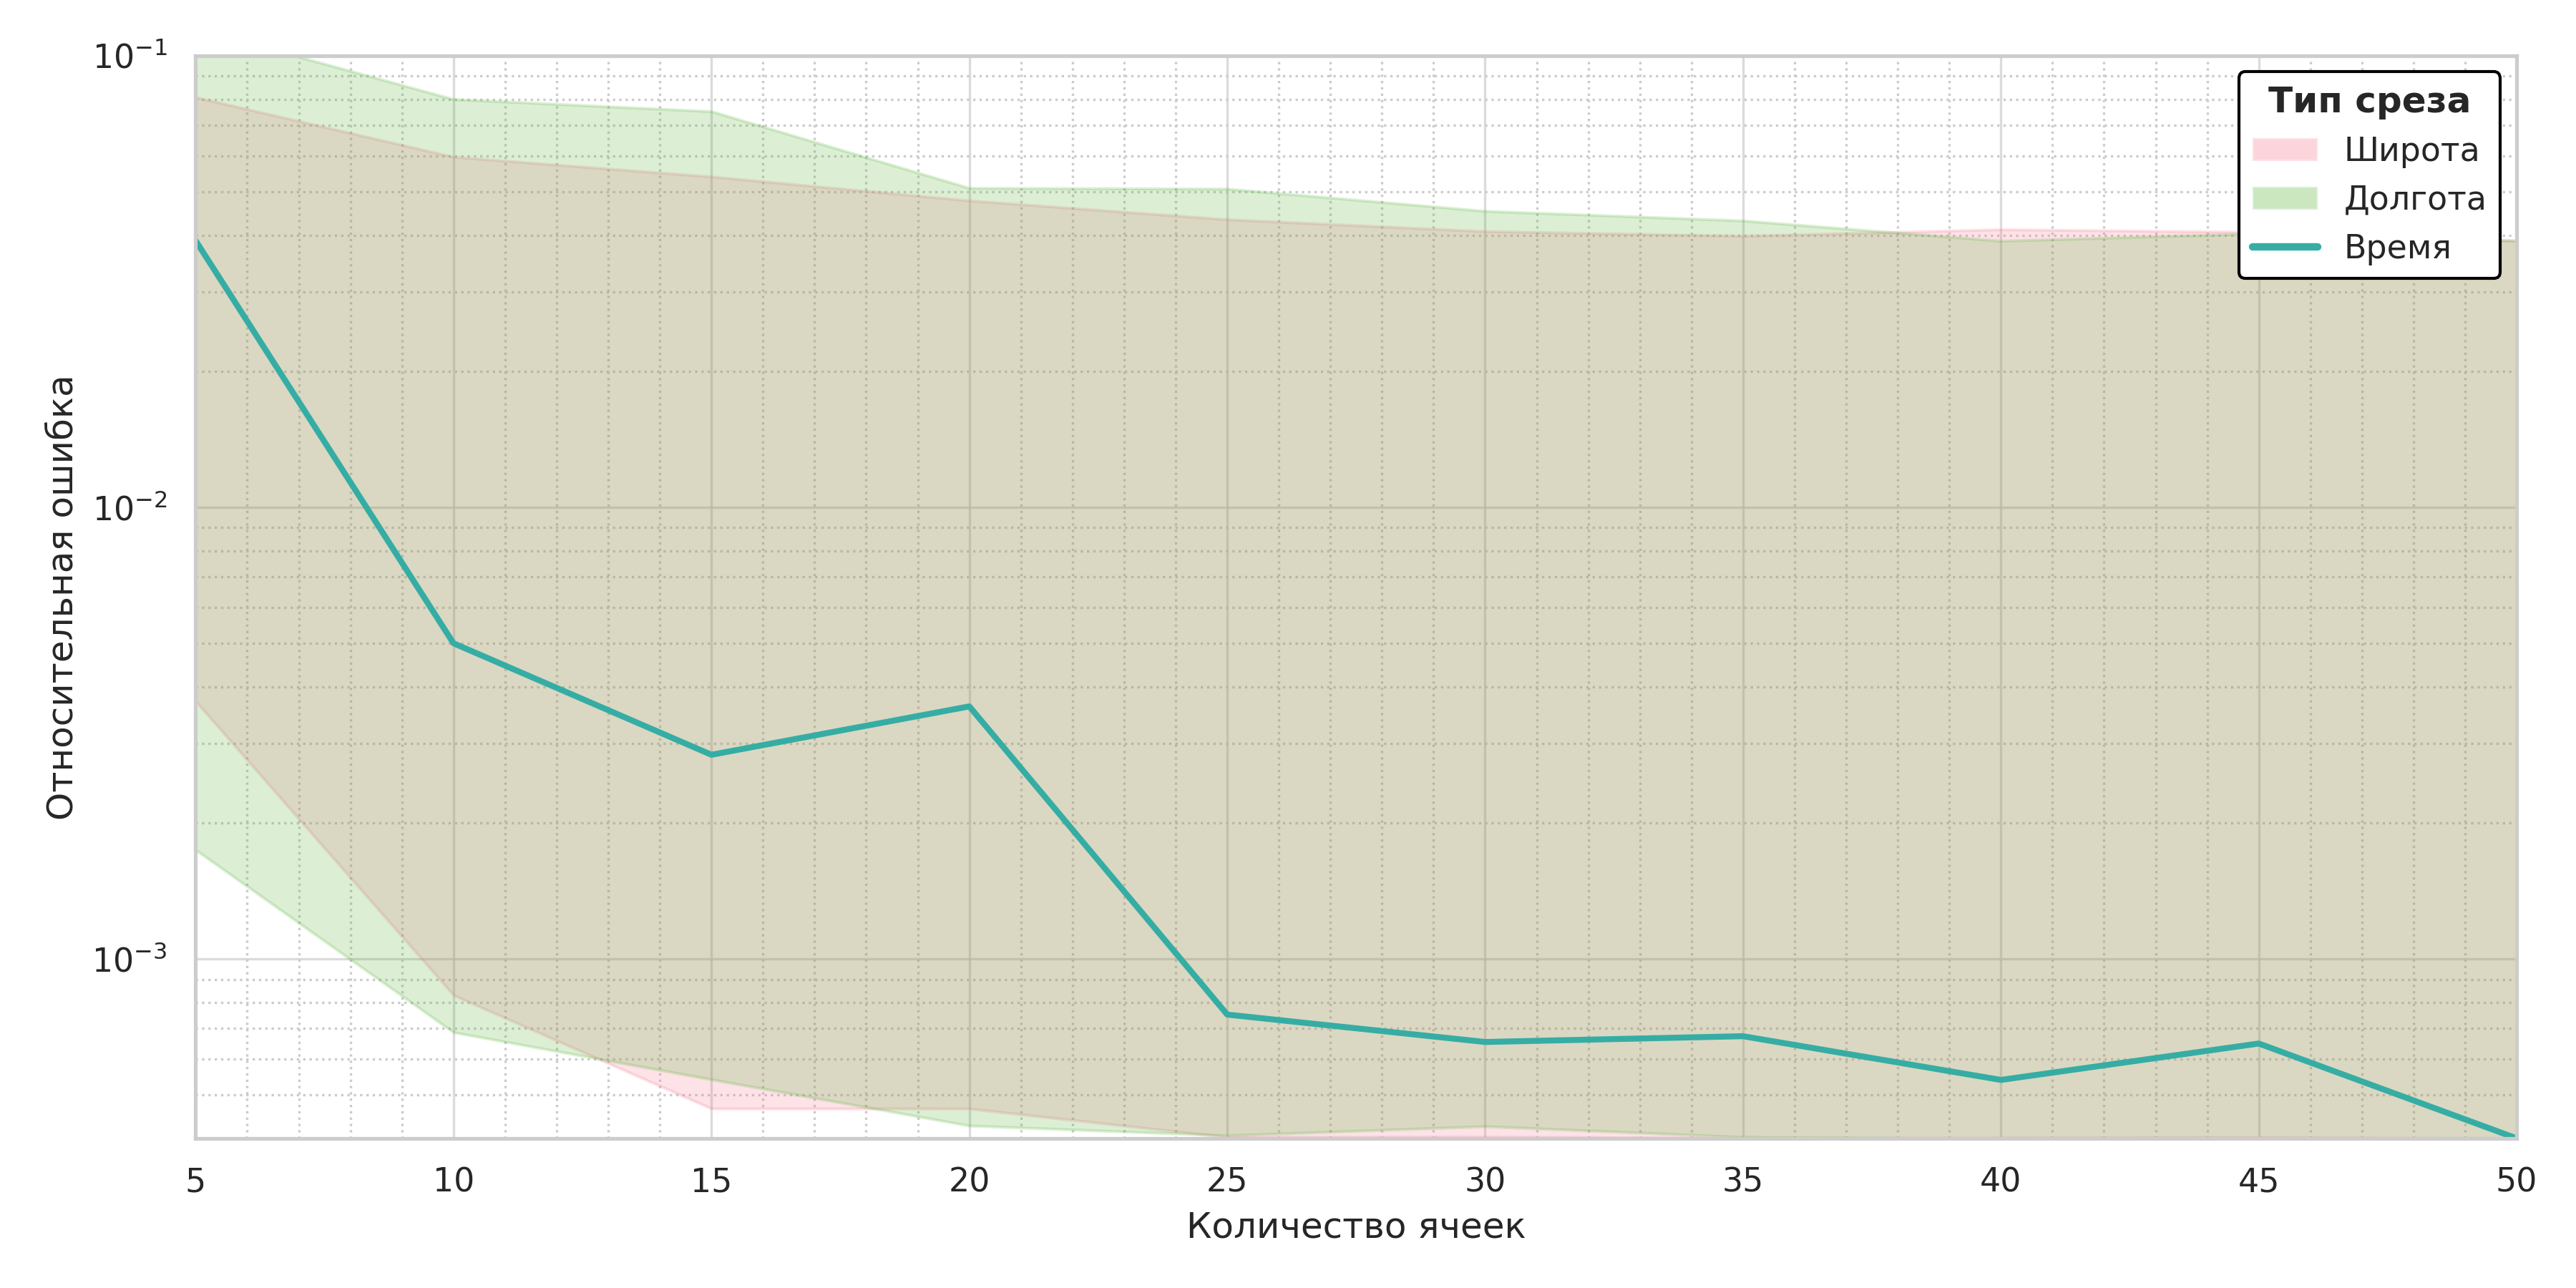
\includegraphics[width=\linewidth]{../images/solution/atmo/2573.png}
    \captionof{figure}{Зависимость ошибки от количества ячеек интерполянта для конфигурации (2, 5, 7, 3)}
    \label{fig:atmo:2573}
 \end{figure}

 \begin{figure}[h!]
    \centering
    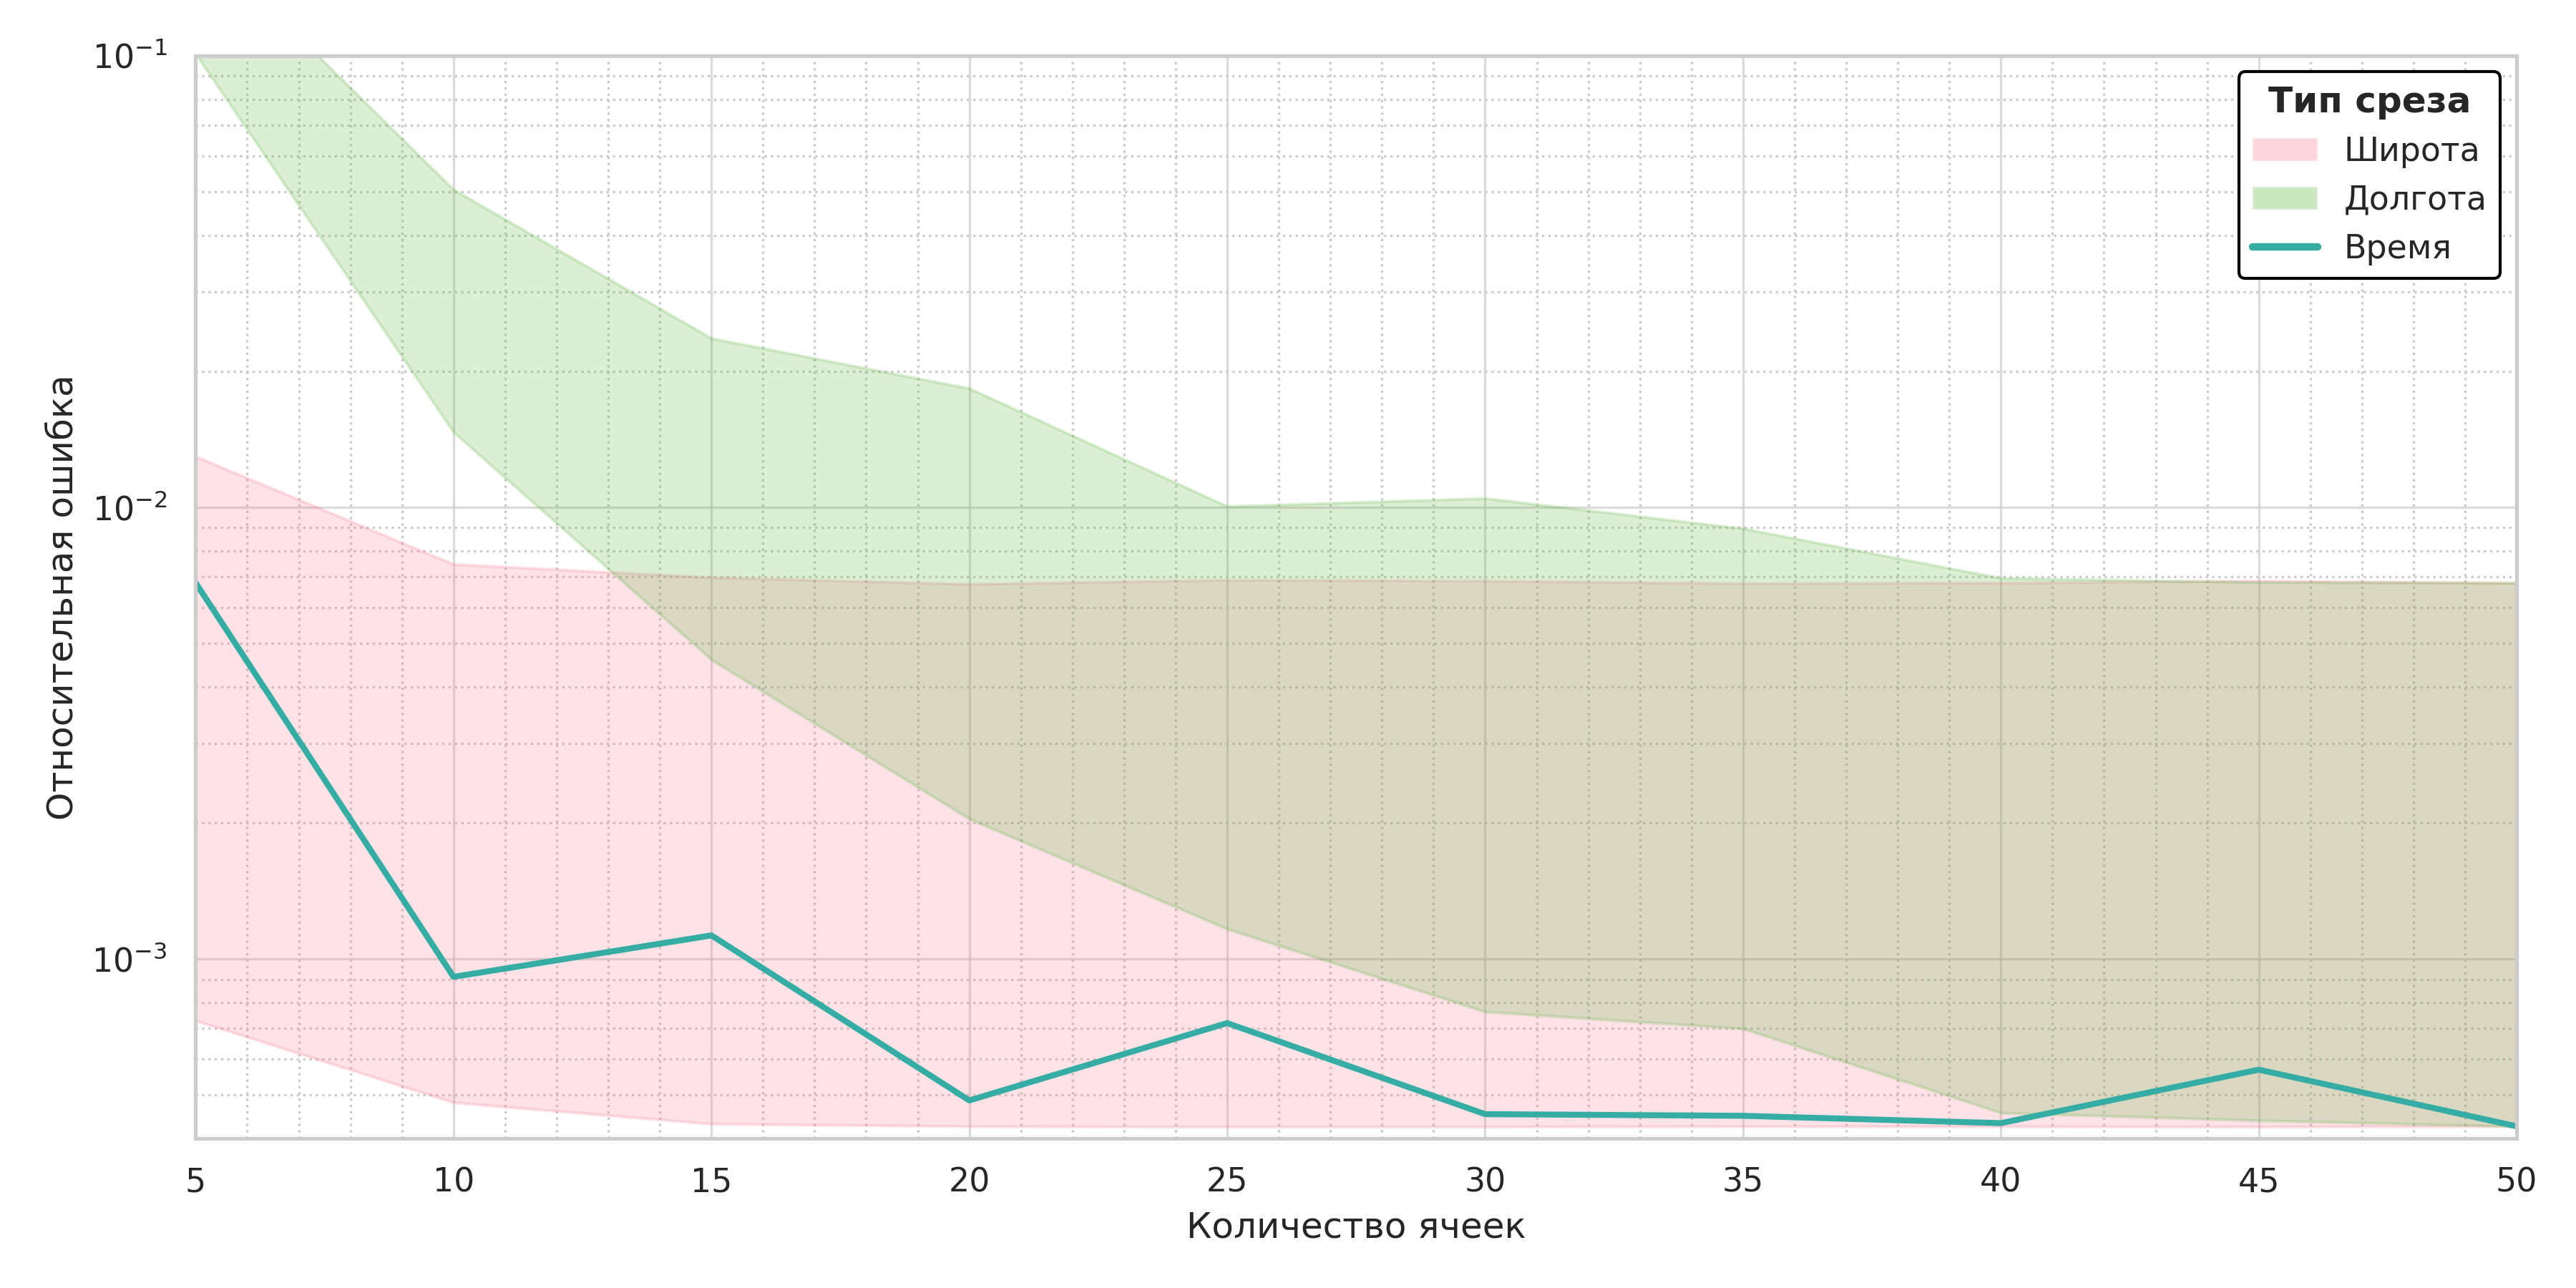
\includegraphics[width=\linewidth]{../images/solution/atmo/2735.png}
    \captionof{figure}{Зависимость ошибки от количества ячеек интерполянта для конфигурации (2, 7, 3, 5)}
    \label{fig:atmo:2735}
 \end{figure}

 \begin{figure}[h!]
    \centering
    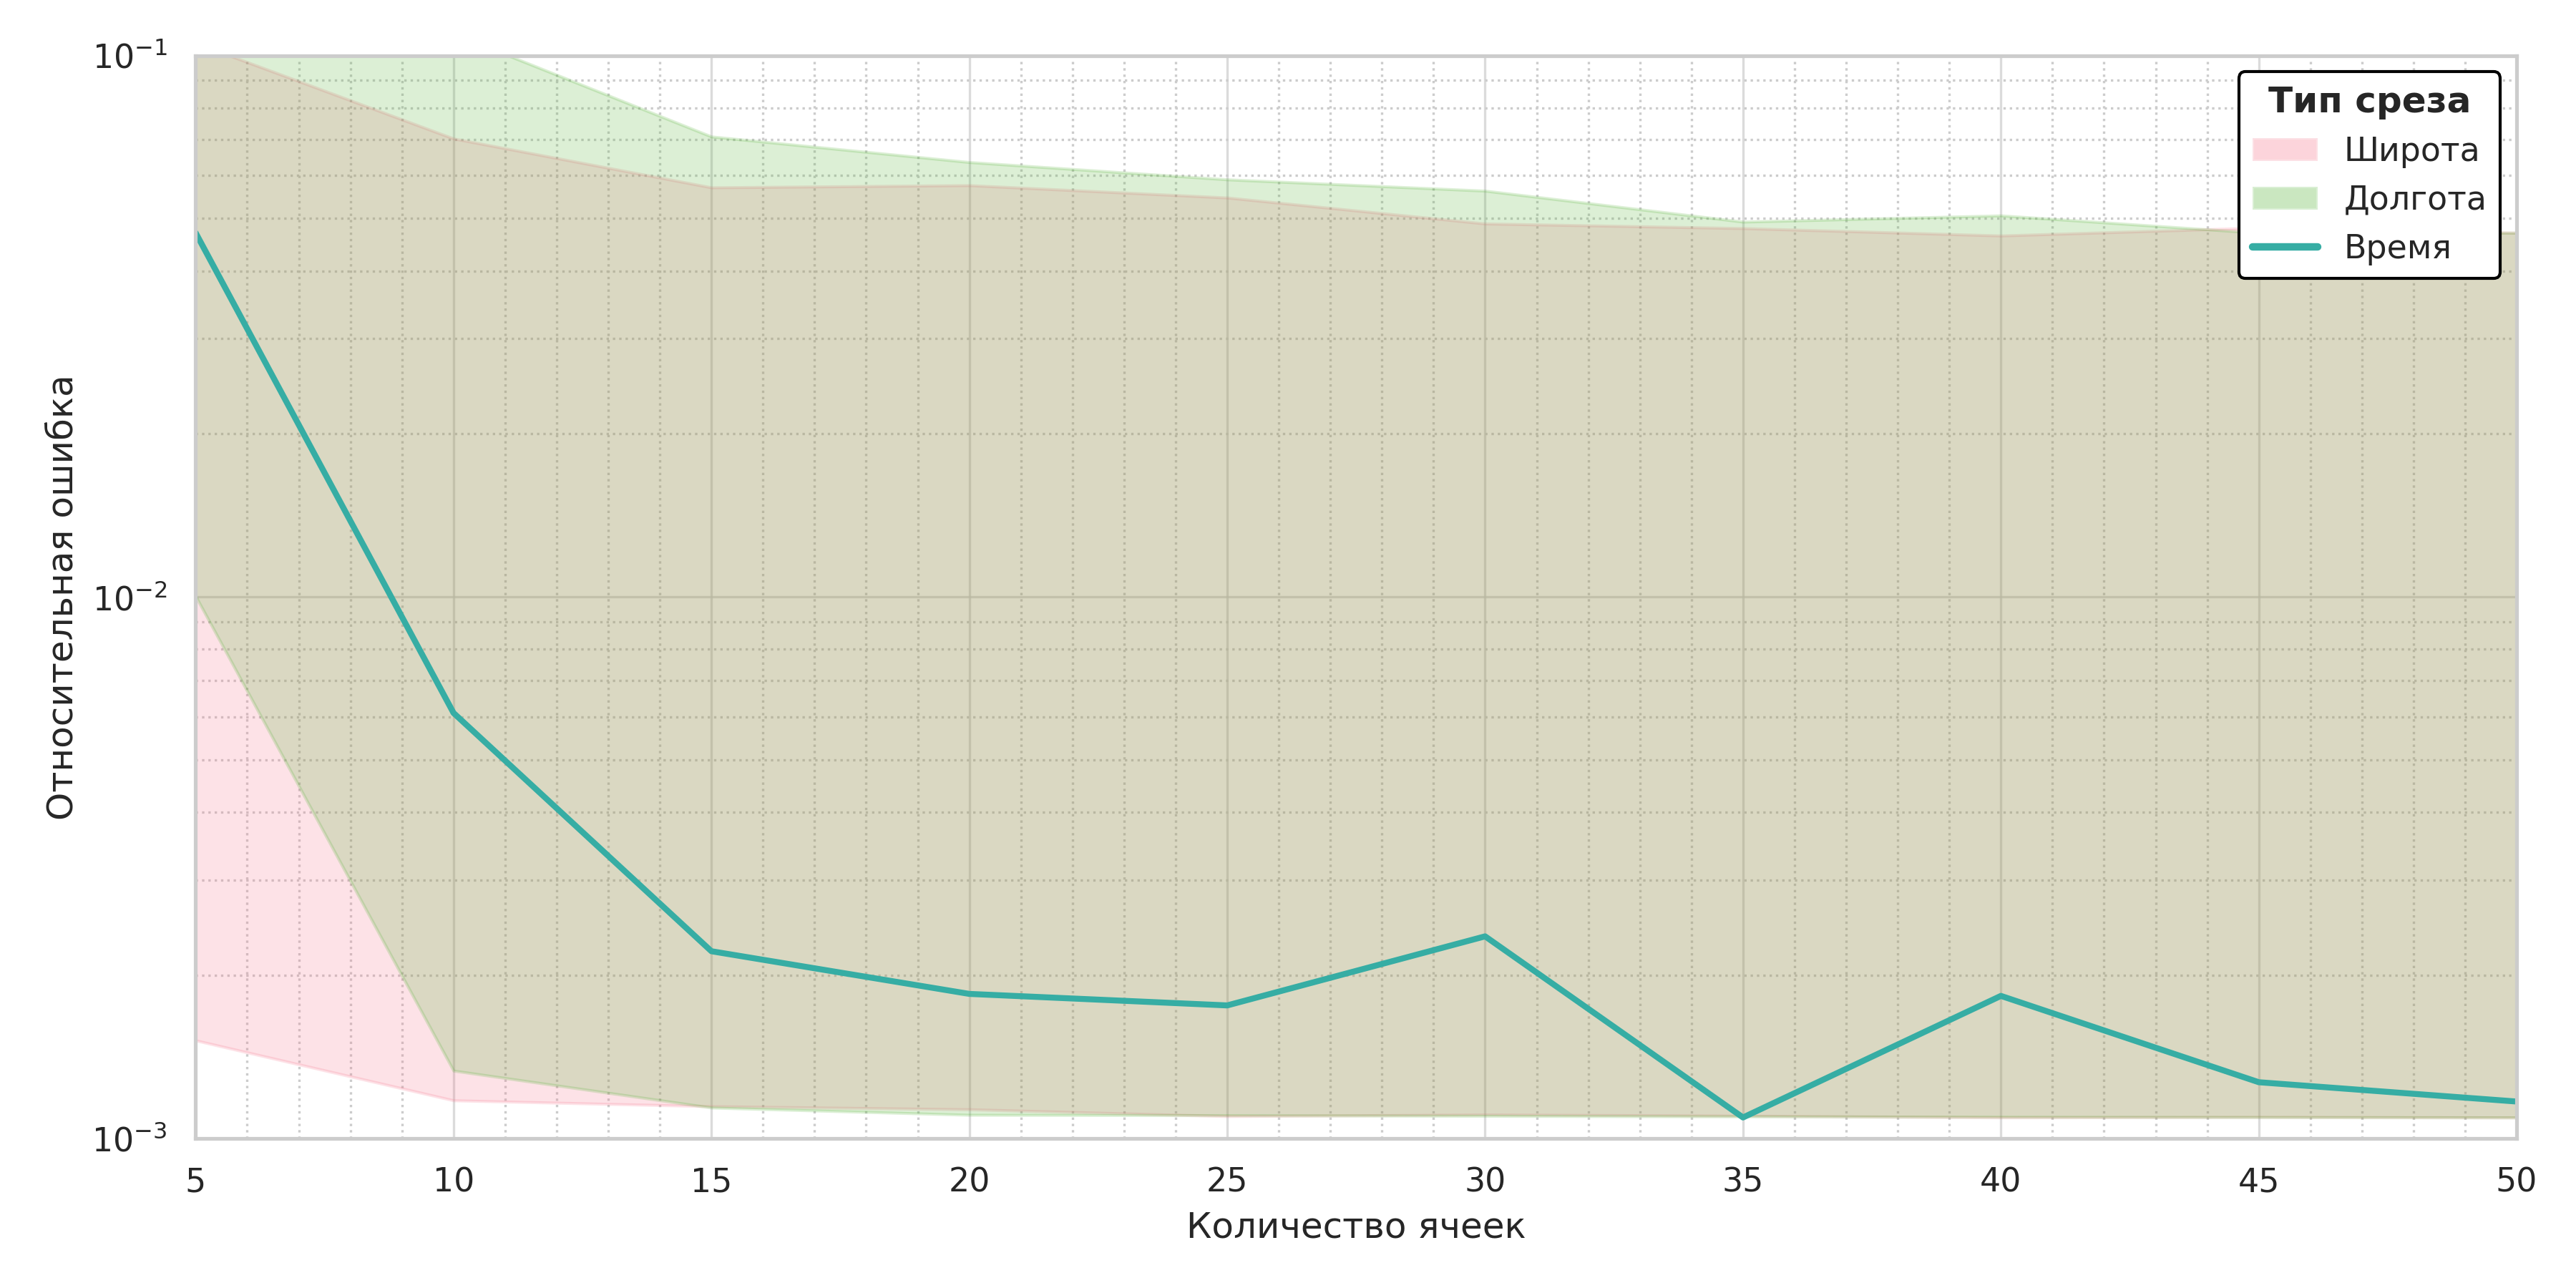
\includegraphics[width=\linewidth]{../images/solution/atmo/2753.png}
    \captionof{figure}{Зависимость ошибки от количества ячеек интерполянта для конфигурации (2, 7, 5, 3)}
    \label{fig:atmo:2753}
 \end{figure}

 Из графиков видно, что максимальная точность интерполянтов в тестах составила $4 \cdot 10^{-4}$.
 По срезам можно определить количество ячеек по каждой координате, которого достаточно для достижения
 предельной точности. Чем больше степень во времени, тем уже диапазон по широте и долготе. Это объясняется тем,
 что для достижения максимальной точности при заданном количестве ячеек по расстоянию
 требуется меньше ячеек по времени. На рисунках \ref{fig:atmo:2357_heatmap} -- \ref{fig:atmo:2753_heatmap} изображены карты
 ошибок для разных конфигураций. Градиент на них направлен вдоль оси, соответствующей
 координате с наименьшей степенью в ячейке.

 Срез по количеству радиальных ячеек отражает тенденцию быстрого спада ошибки в области
 10 -- 30 и замедления спада далее. В окретсности 65 угол наклона графика мал, следовательно,
 выбор начального приближения количества ячеек был верным.

 \begin{figure}[h!]
    \centering
    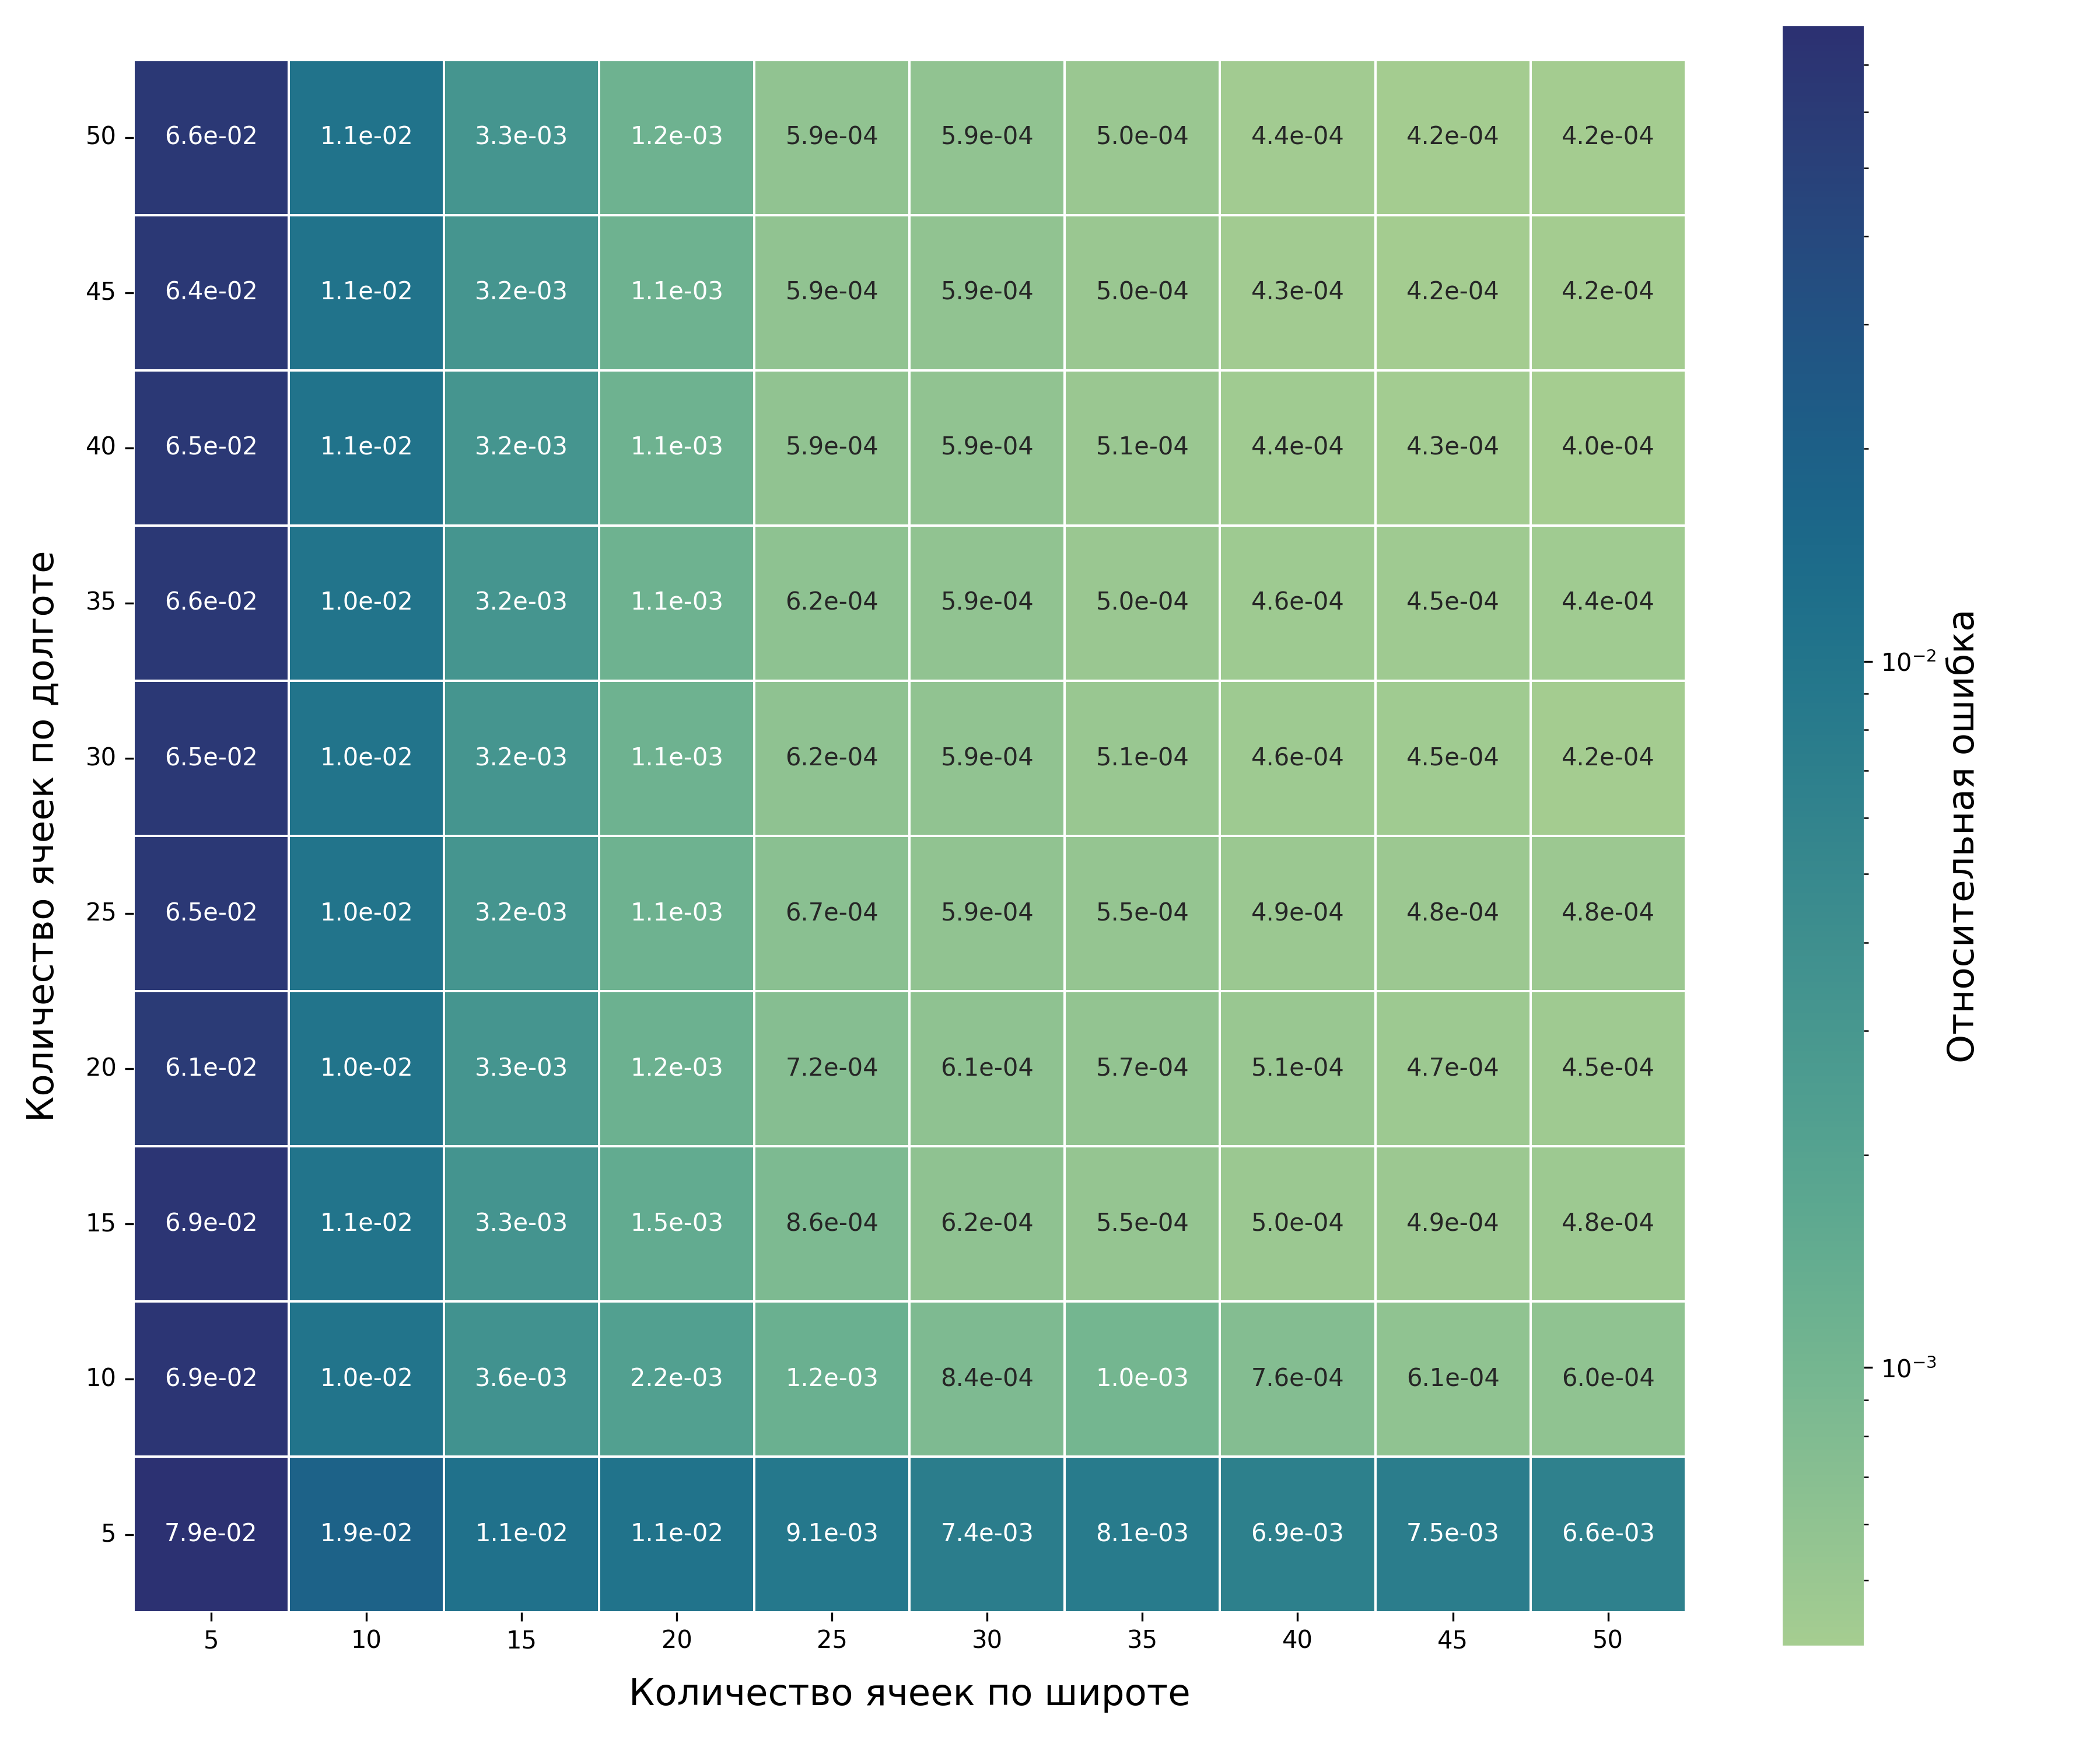
\includegraphics[width=0.85\linewidth]{../images/solution/atmo/2357_heatmap.png}
    \captionof{figure}{Карта ошибок для конфигурации (2, 3, 5, 7)}
    \label{fig:atmo:2357_heatmap}
 \end{figure}

 \begin{figure}[h!]
    \centering
    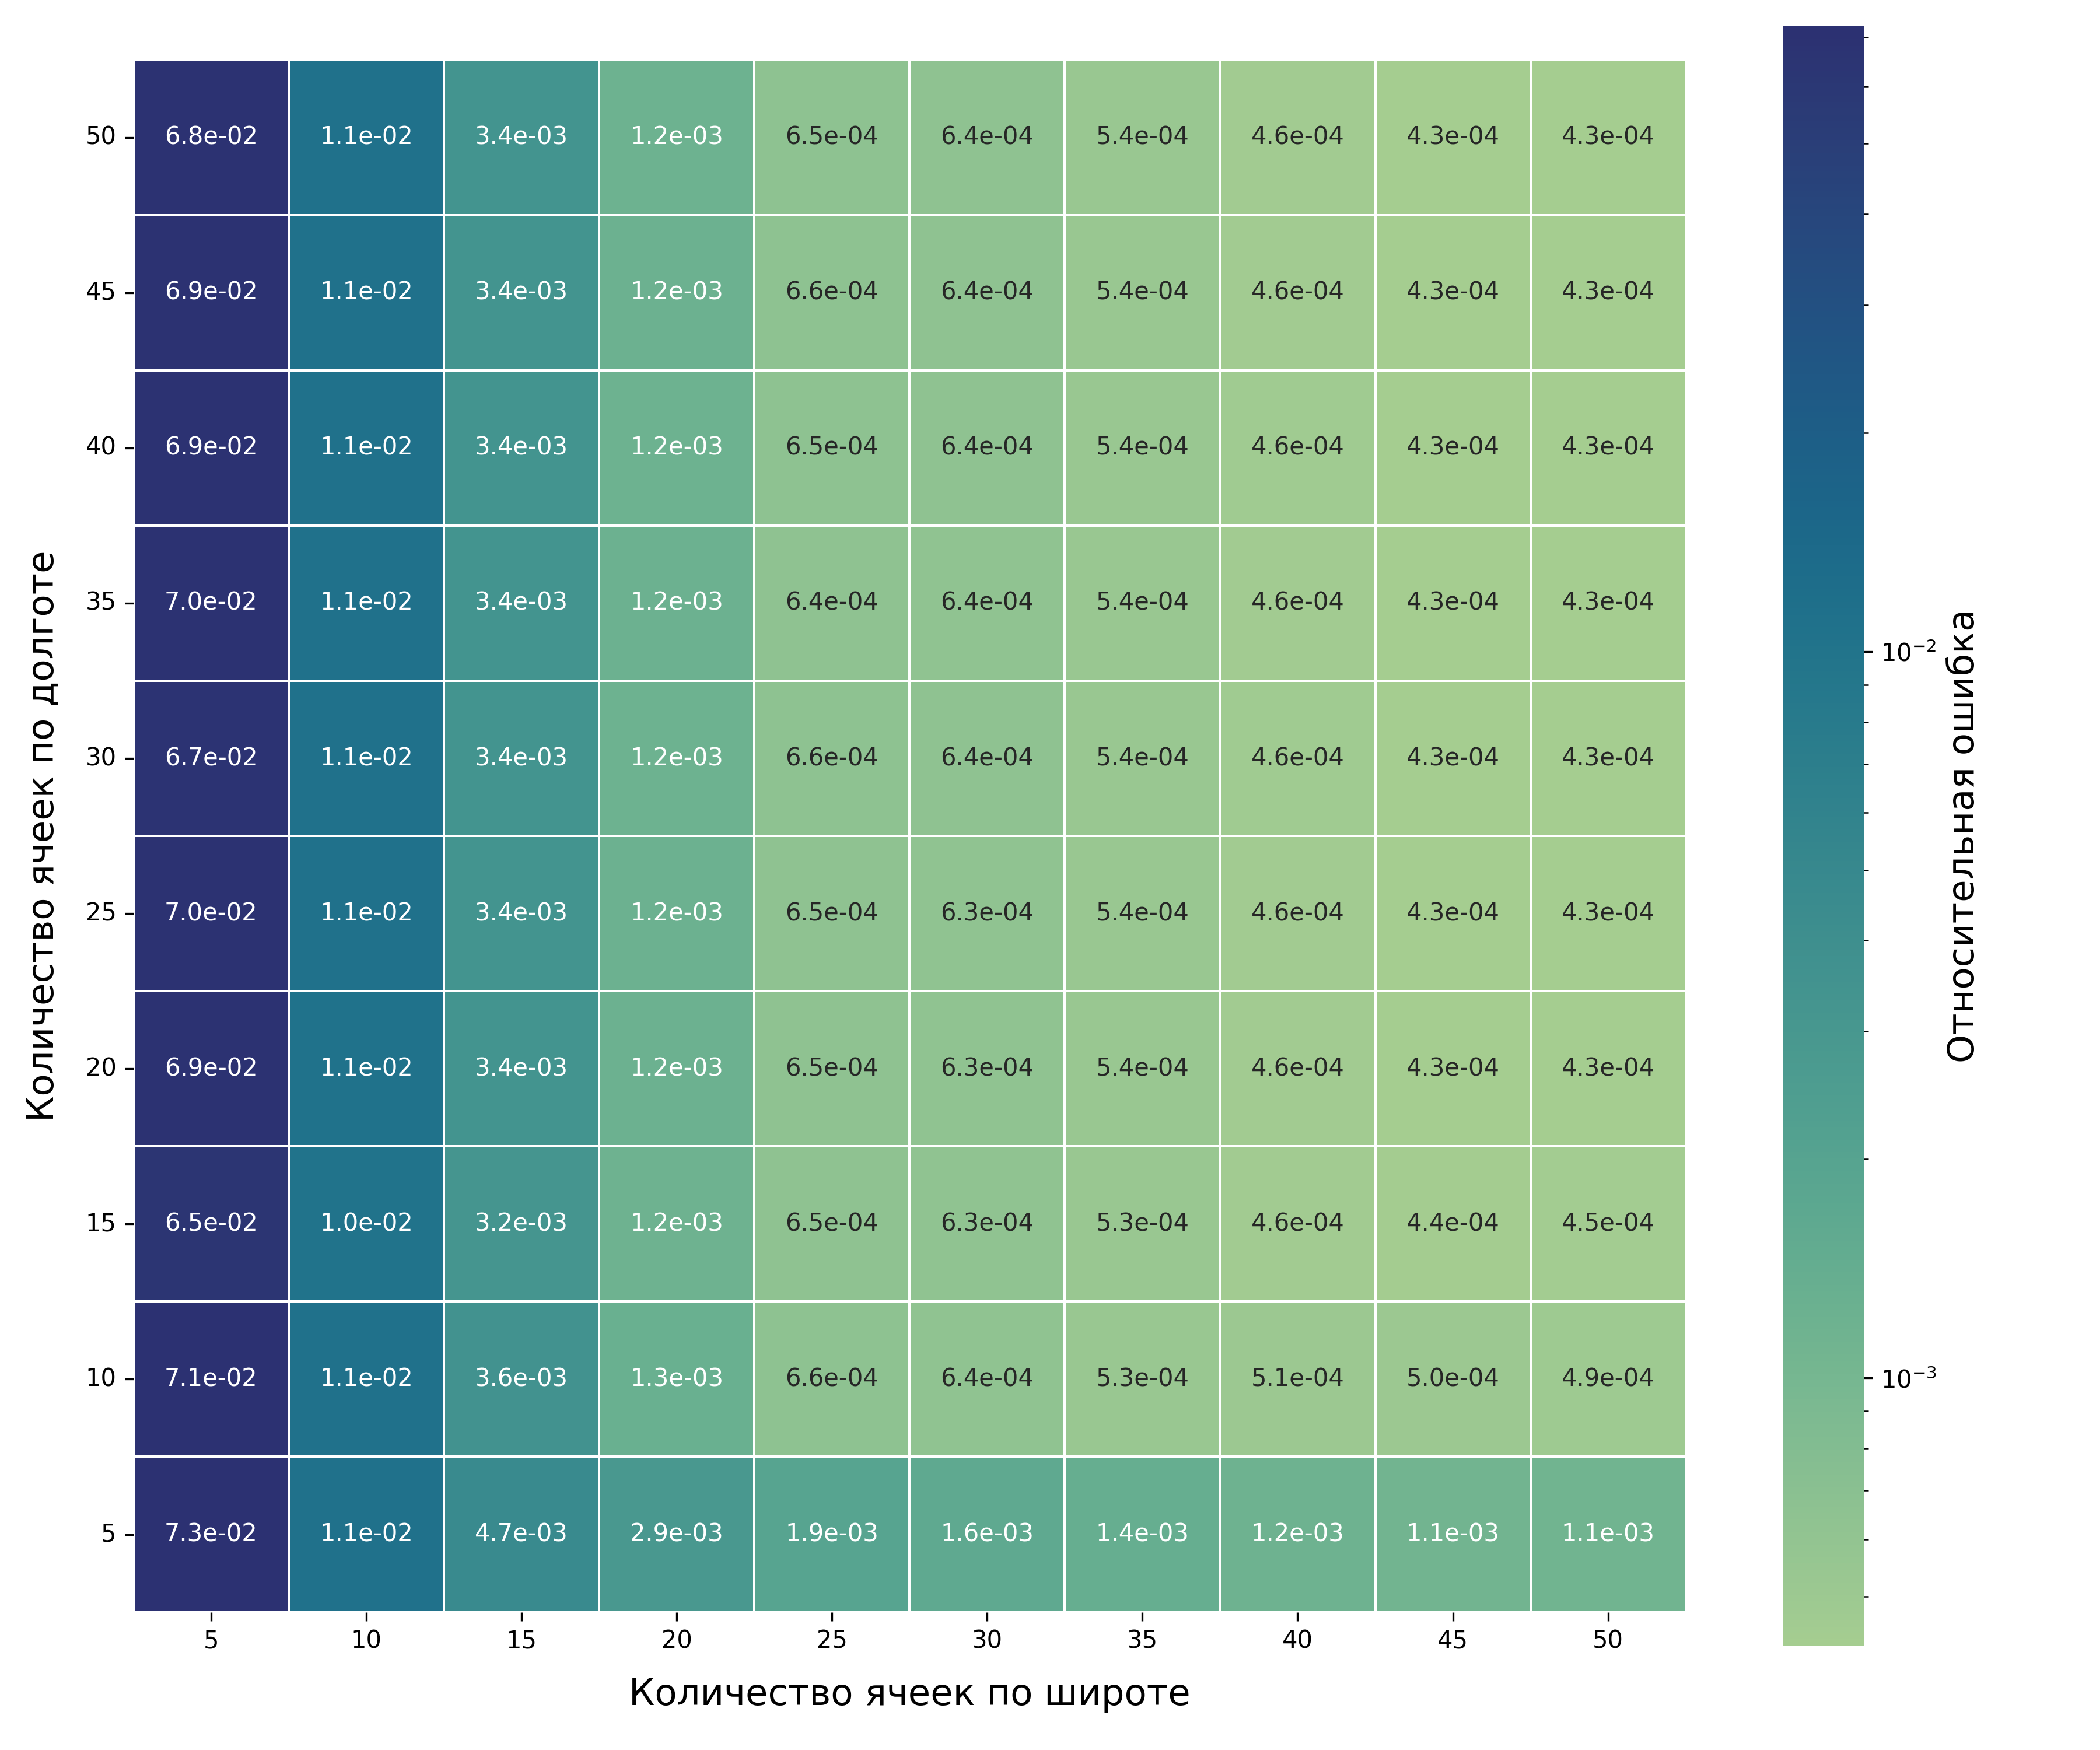
\includegraphics[width=0.85\linewidth]{../images/solution/atmo/2375_heatmap.png}
    \captionof{figure}{Карта ошибок для конфигурации (2, 3, 7, 5)}
    \label{fig:atmo:2375_heatmap}
 \end{figure}

 \begin{figure}[h!]
    \centering
    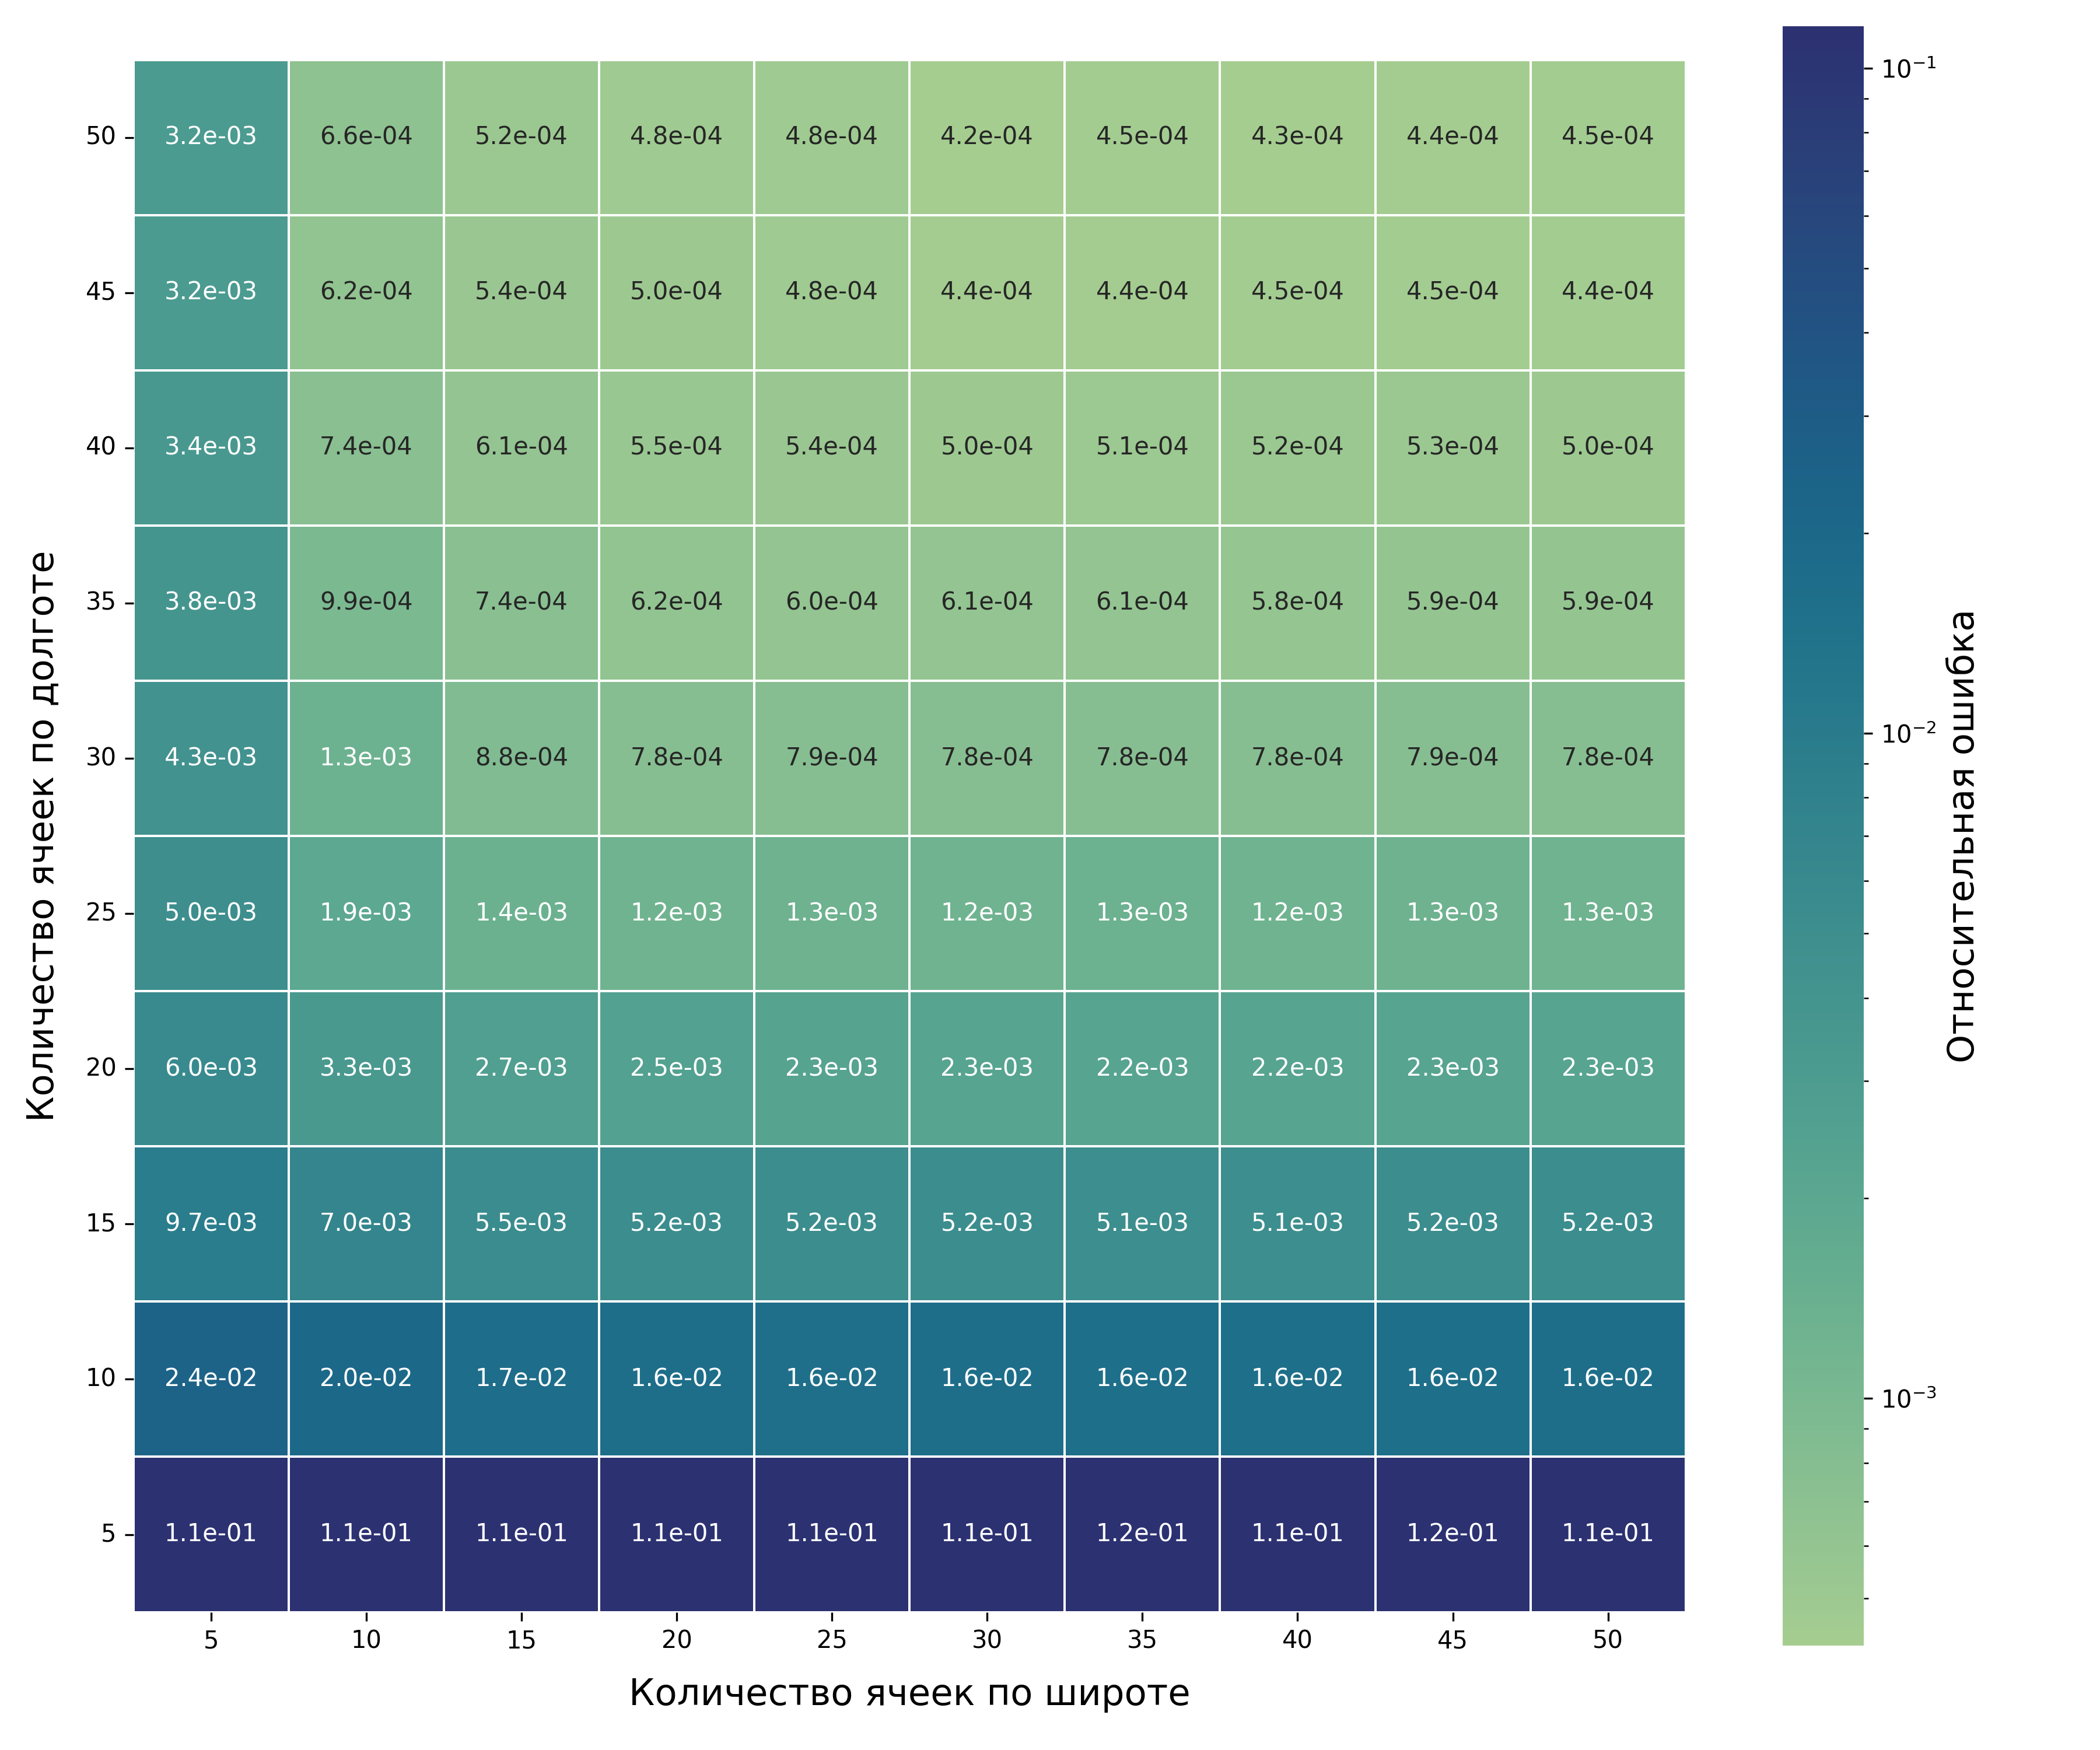
\includegraphics[width=0.85\linewidth]{../images/solution/atmo/2537_heatmap.png}
    \captionof{figure}{Карта ошибок для конфигурации (2, 5, 3, 7)}
    \label{fig:atmo:2537_heatmap}
 \end{figure}

 \begin{figure}[h!]
    \centering
    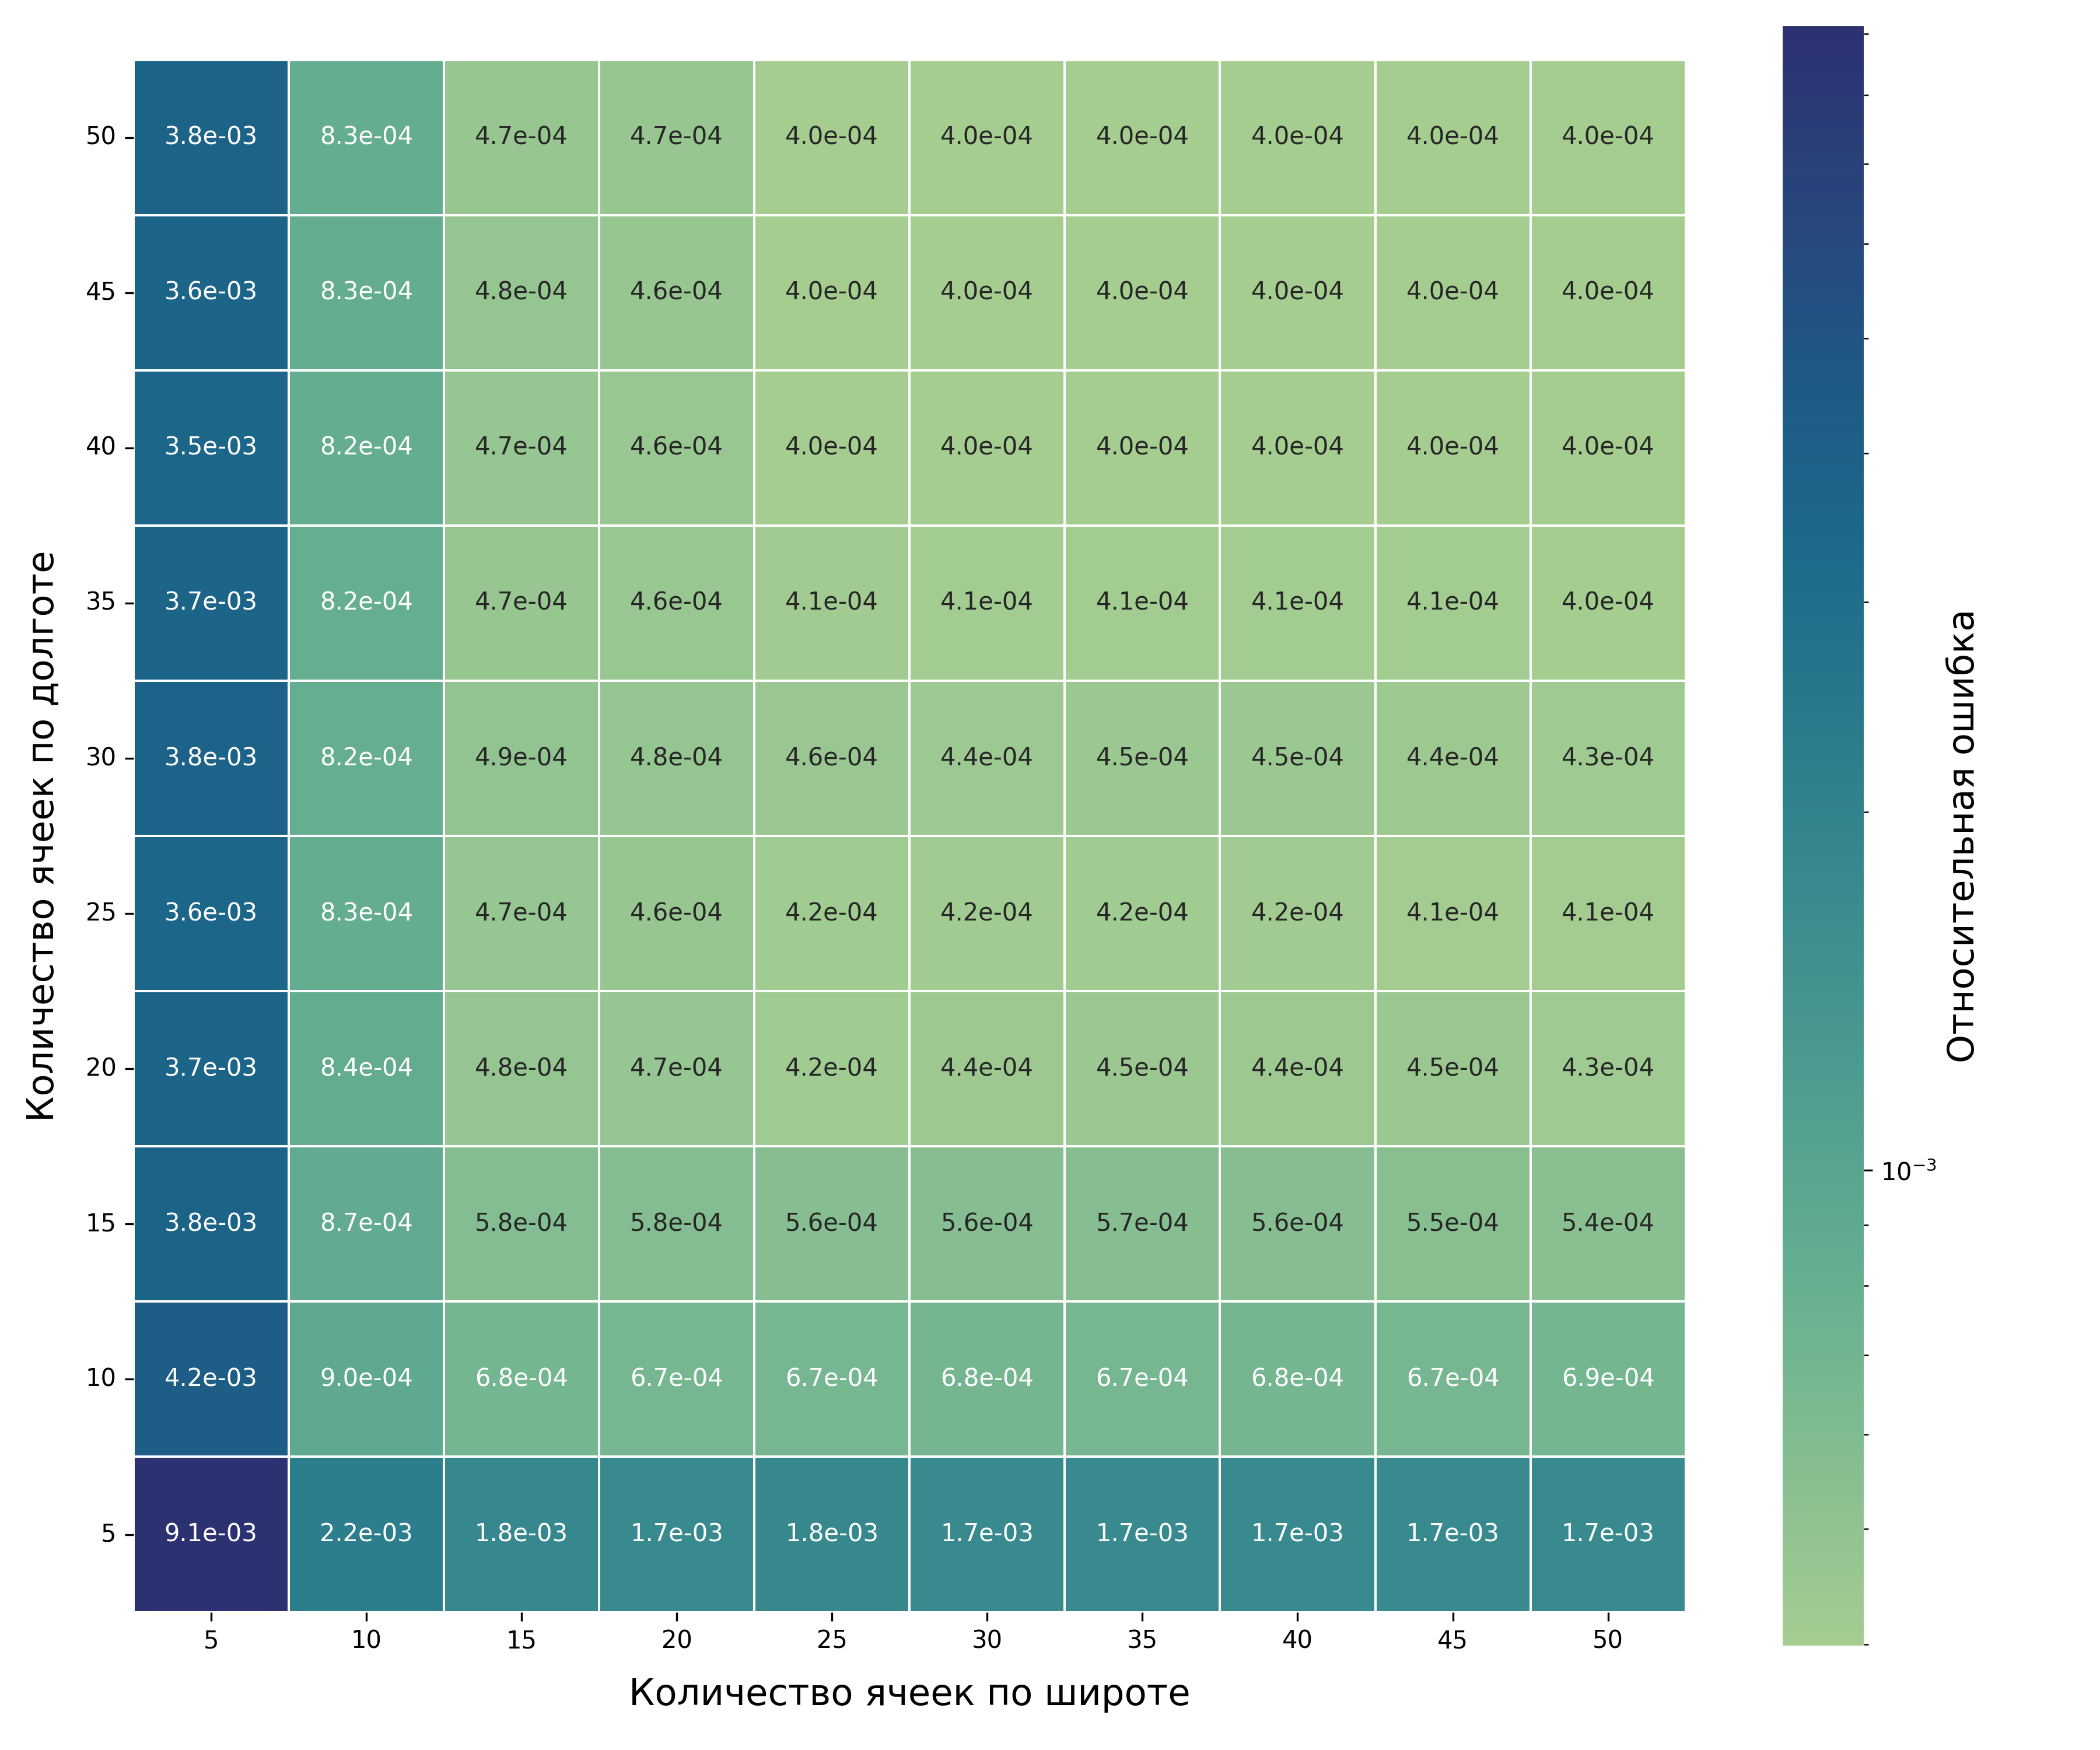
\includegraphics[width=0.85\linewidth]{../images/solution/atmo/2573_heatmap.png}
    \captionof{figure}{Карта ошибок для конфигурации (2, 5, 7, 3)}
    \label{fig:atmo:2573_heatmap}
 \end{figure}

 \begin{figure}[h!]
    \centering
    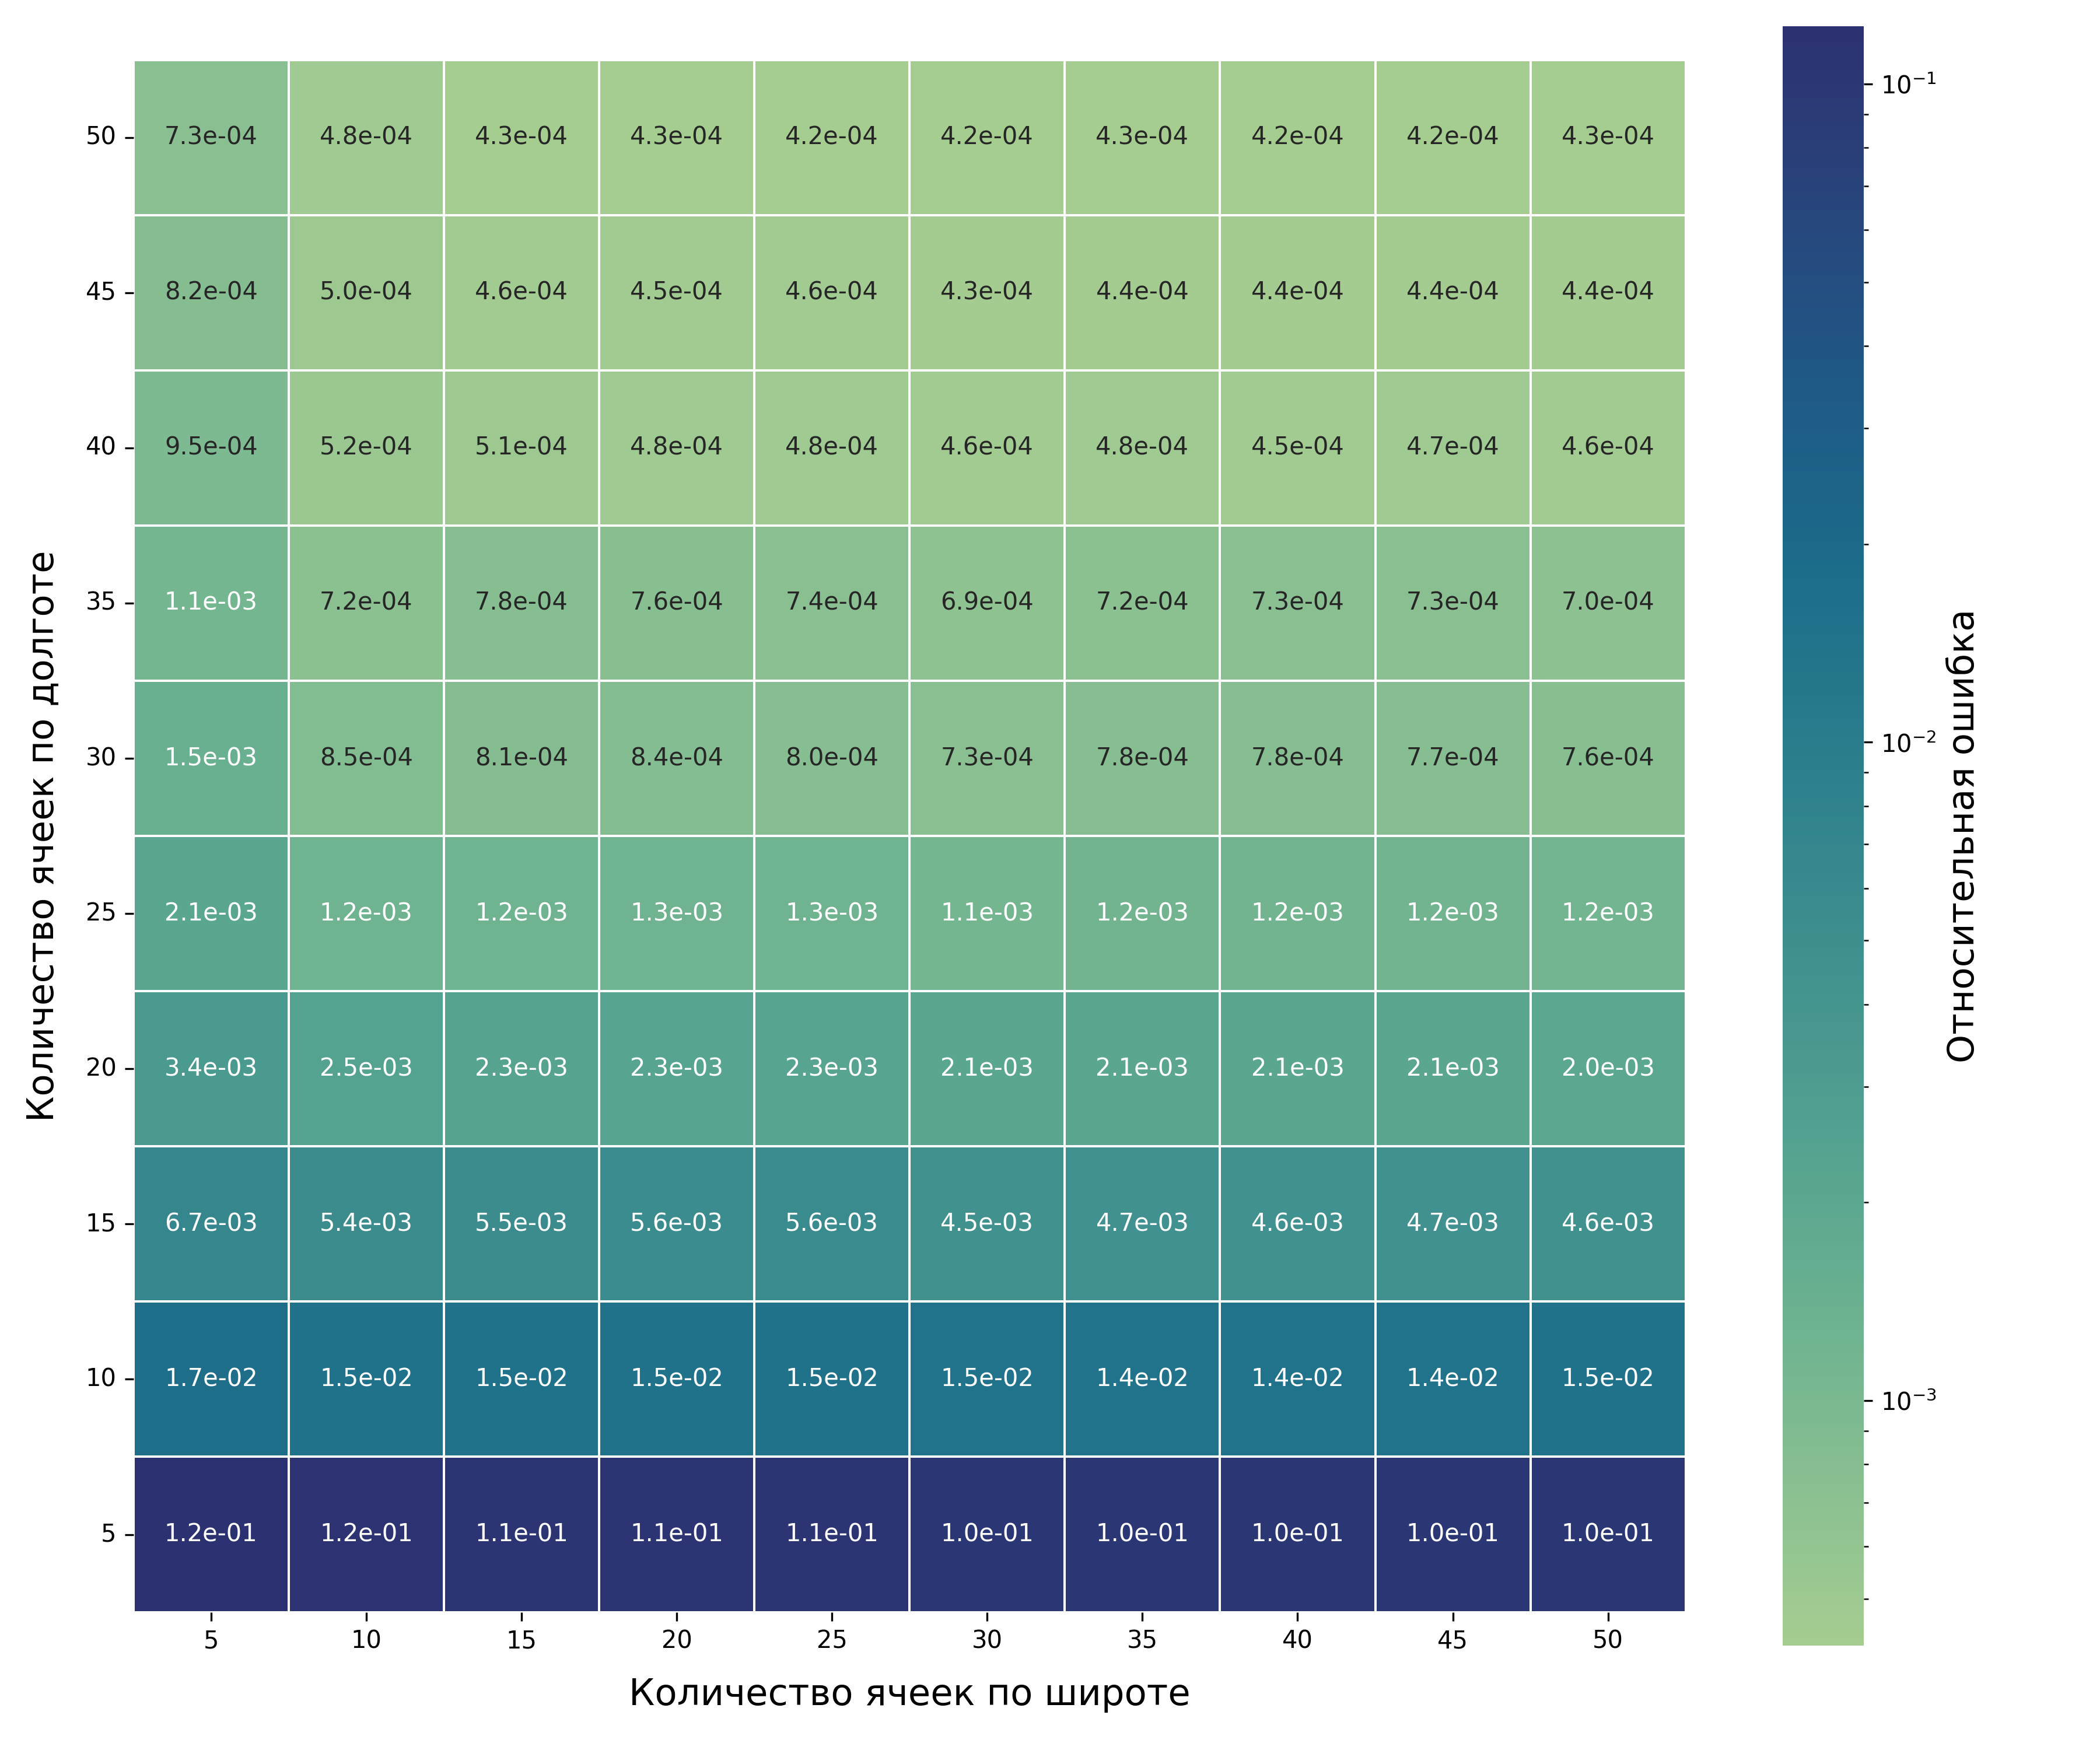
\includegraphics[width=0.85\linewidth]{../images/solution/atmo/2735_heatmap.png}
    \captionof{figure}{Карта ошибок для конфигурации (2, 7, 3, 5)}
    \label{fig:atmo:2735_heatmap}
 \end{figure}

 \begin{figure}[h!]
    \centering
    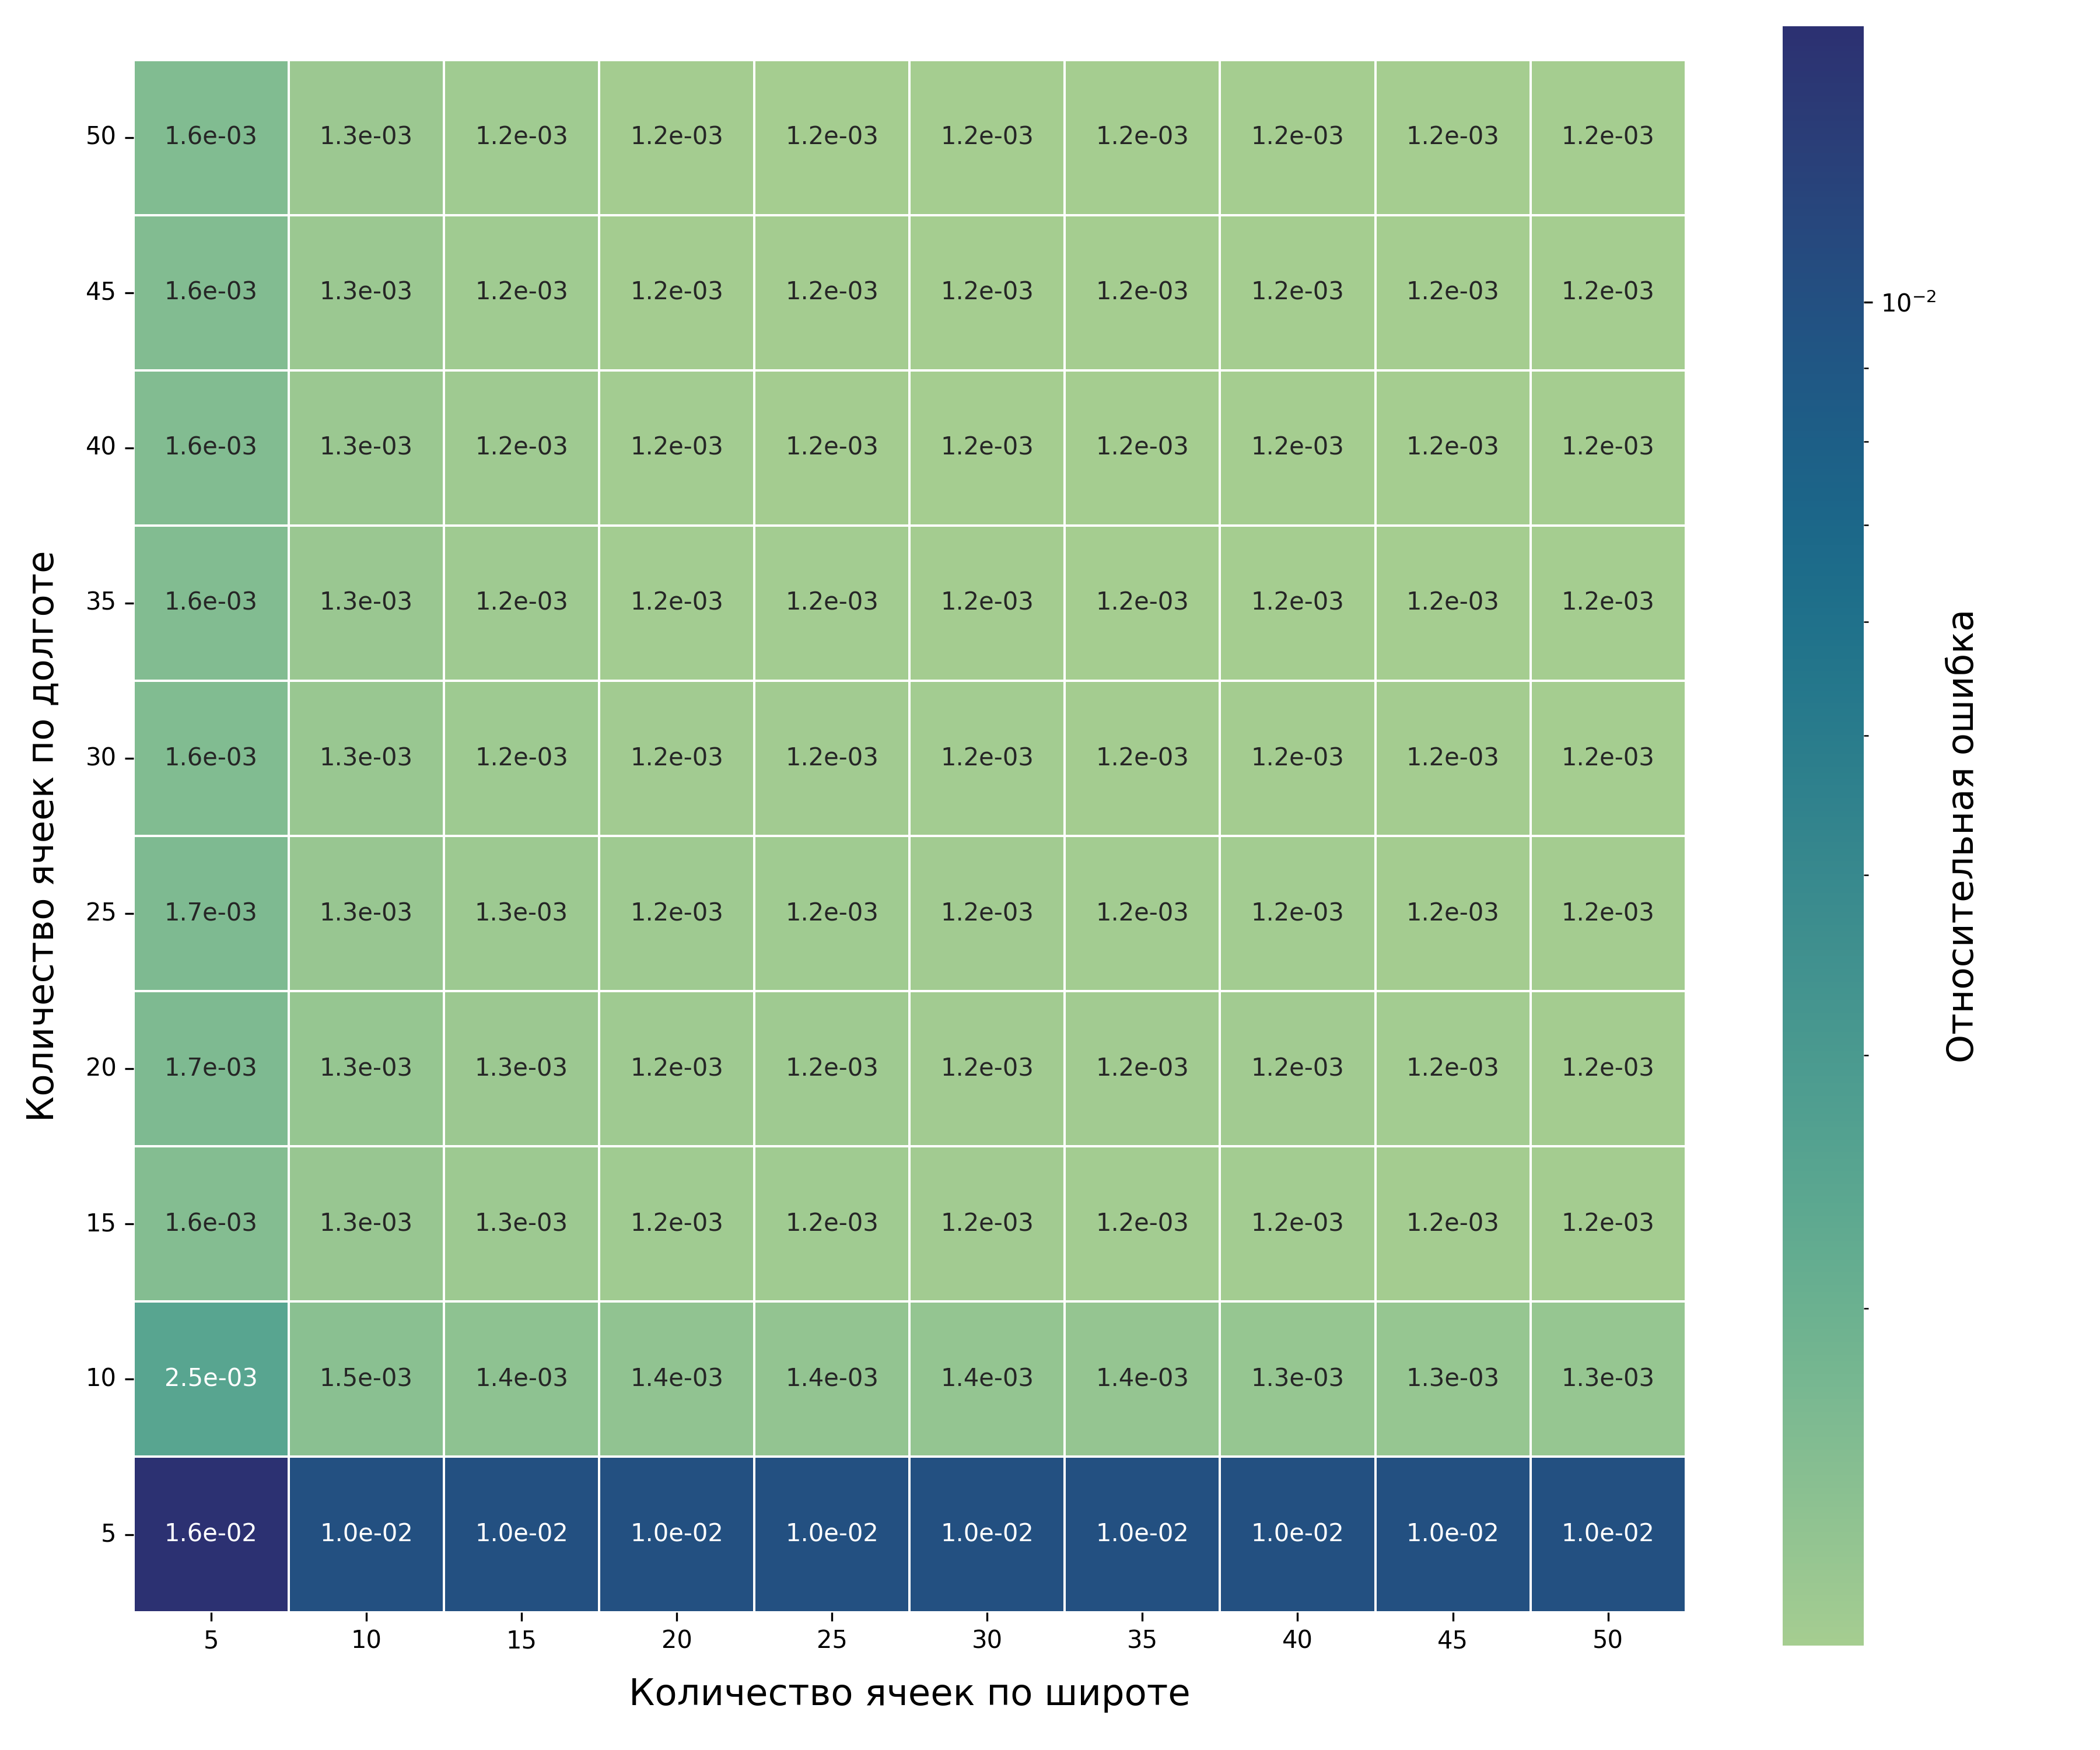
\includegraphics[width=0.85\linewidth]{../images/solution/atmo/2753_heatmap.png}
    \captionof{figure}{Карта ошибок для конфигурации (2, 7, 5, 3)}
    \label{fig:atmo:2753_heatmap}
 \end{figure}

 \begin{figure}[h!]
    \centering
    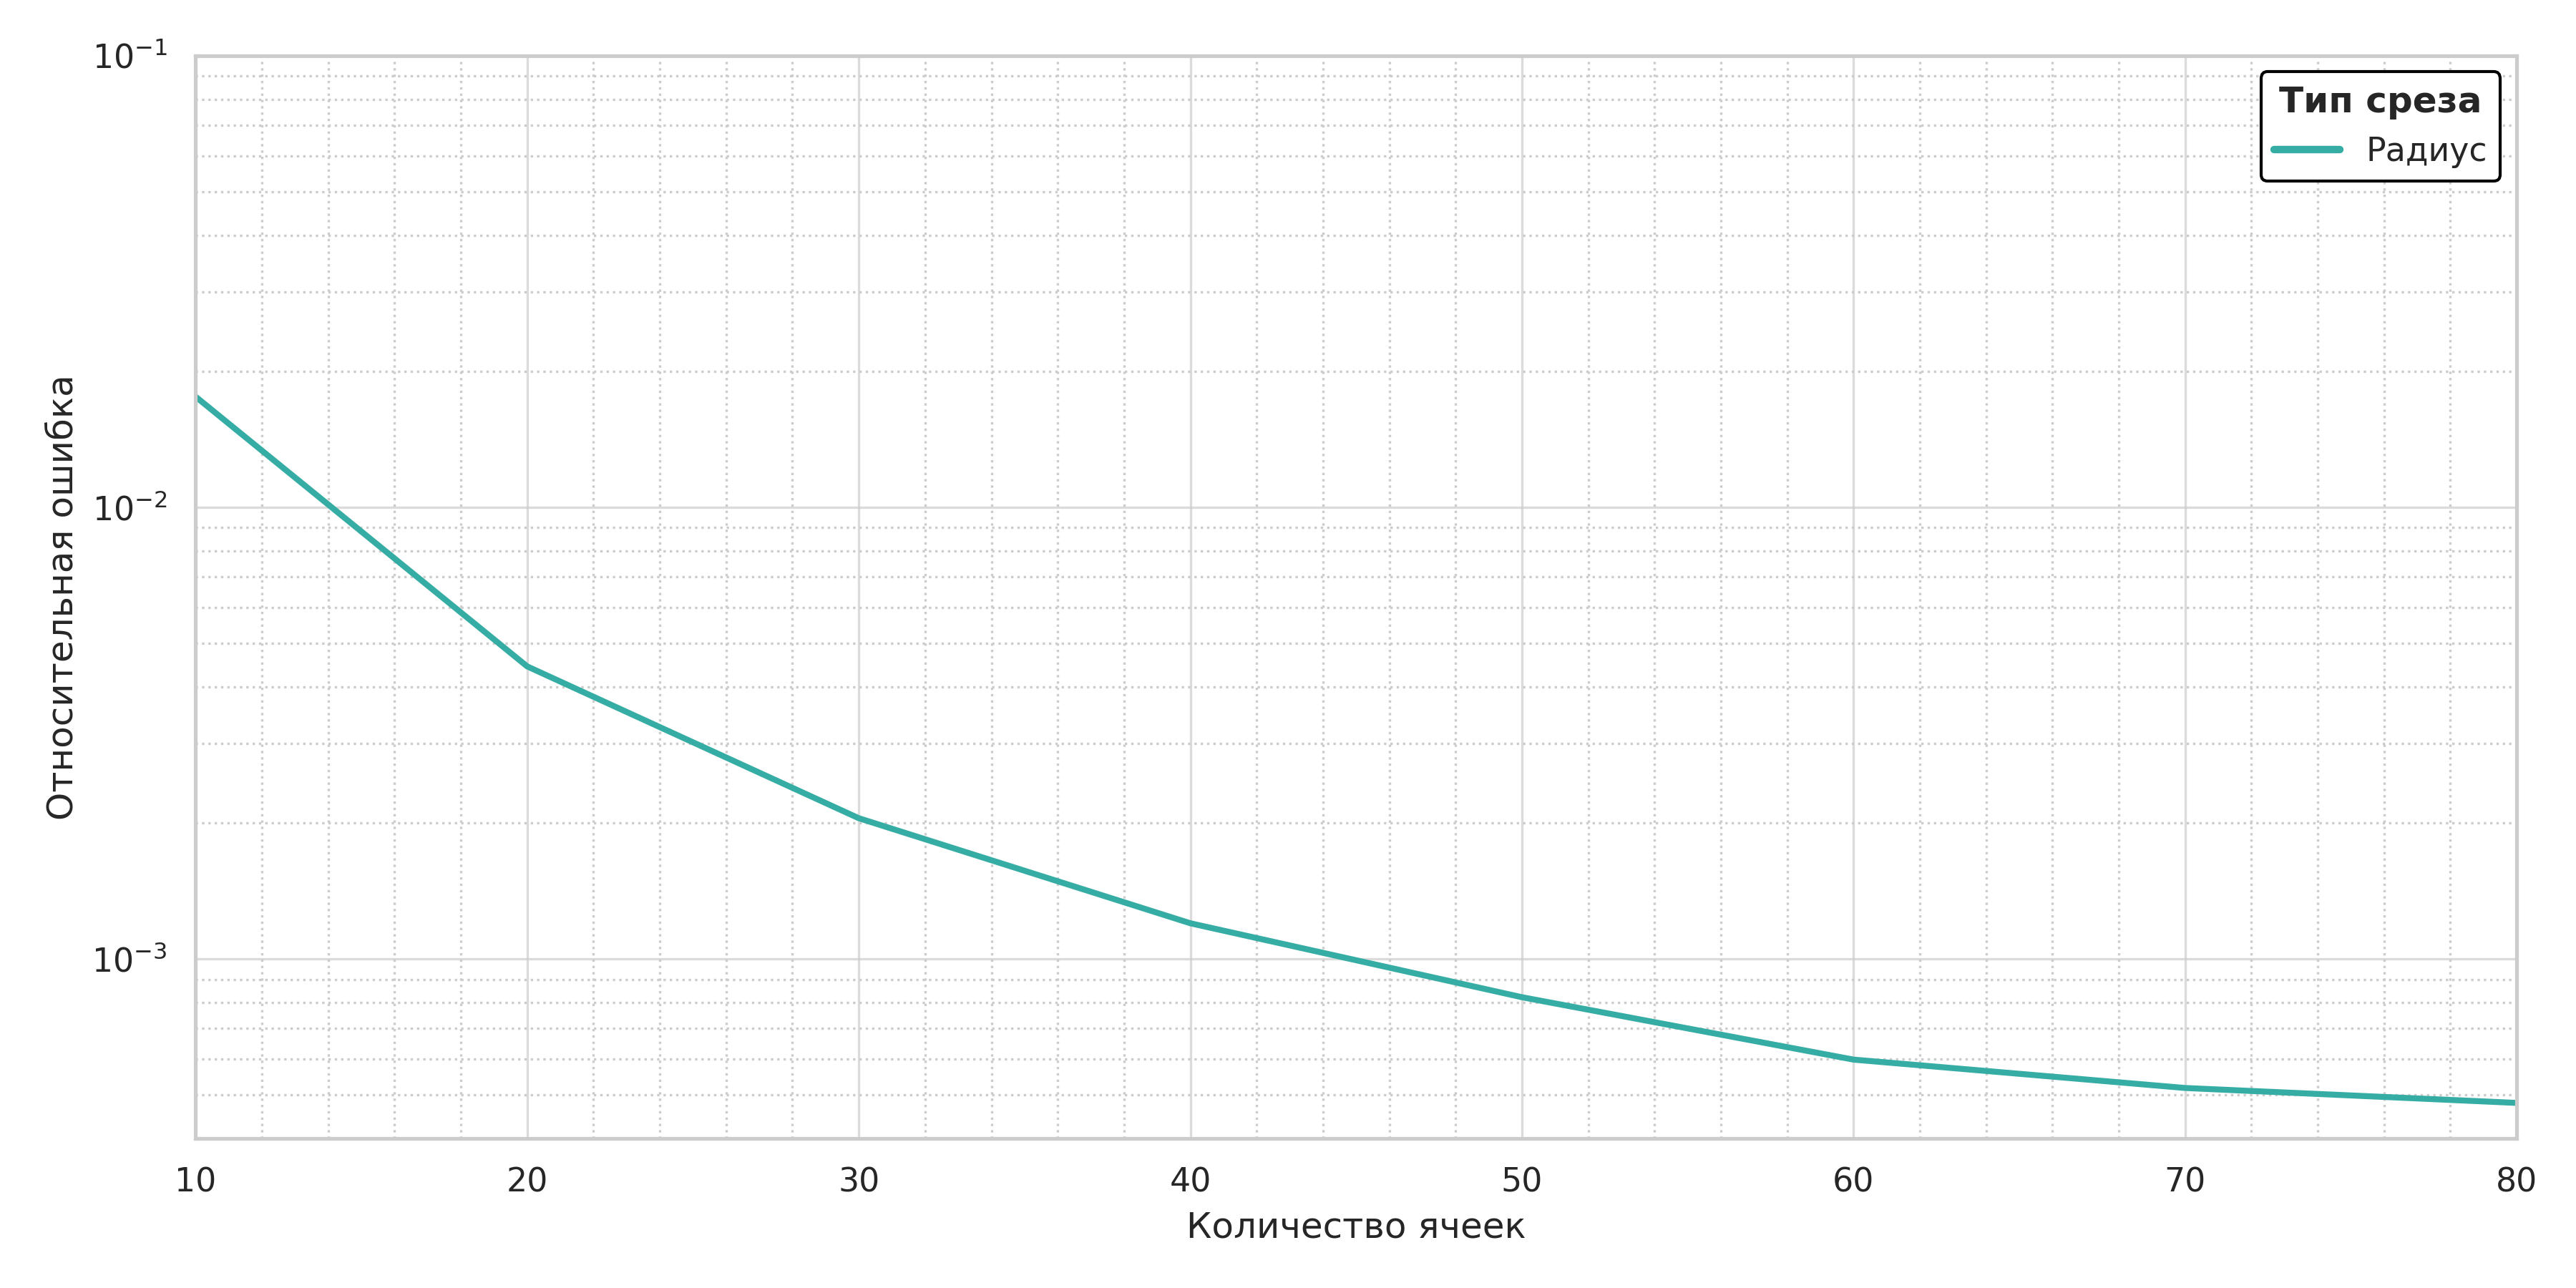
\includegraphics[width=\linewidth]{../images/solution/atmo/2357_rho.png}
    \captionof{figure}{Зависимость ошибки от количества ячеек интерполянта по радиусу для конфигурации (2, 3, 5, 7)}
    \label{fig:atmo:2357_rho}
 \end{figure}

 На картах \ref{fig:atmo:2753_latlon} и \ref{fig:atmo:2753_latlon_abs_err} приведено
 распределение плотности и абсолютной ошибки соответственно для интерполянта на высоте 350 километров.
 Использовалась конфигурация (2, 7, 5, 3) с количеством ячеек (65, 50, 50, 50). Темные участки, относящиеся к областям с
 повышенной плотностью, совпадают с участками, на которых интерполяция дает наибольшую абсолютную ошибку.
 В то же время относительная ошибка меняется по области не существенно. Темное пятно в левой
 части графика соответствуют положению, находящемуся под прямыми солнечными лучами.
 Темные полосы на рисунке \ref{fig:atmo:2753_latlon_abs_err} возникают на границе ячеек
 по широте и долготе. 

 \begin{figure}[h!]
    \centering
    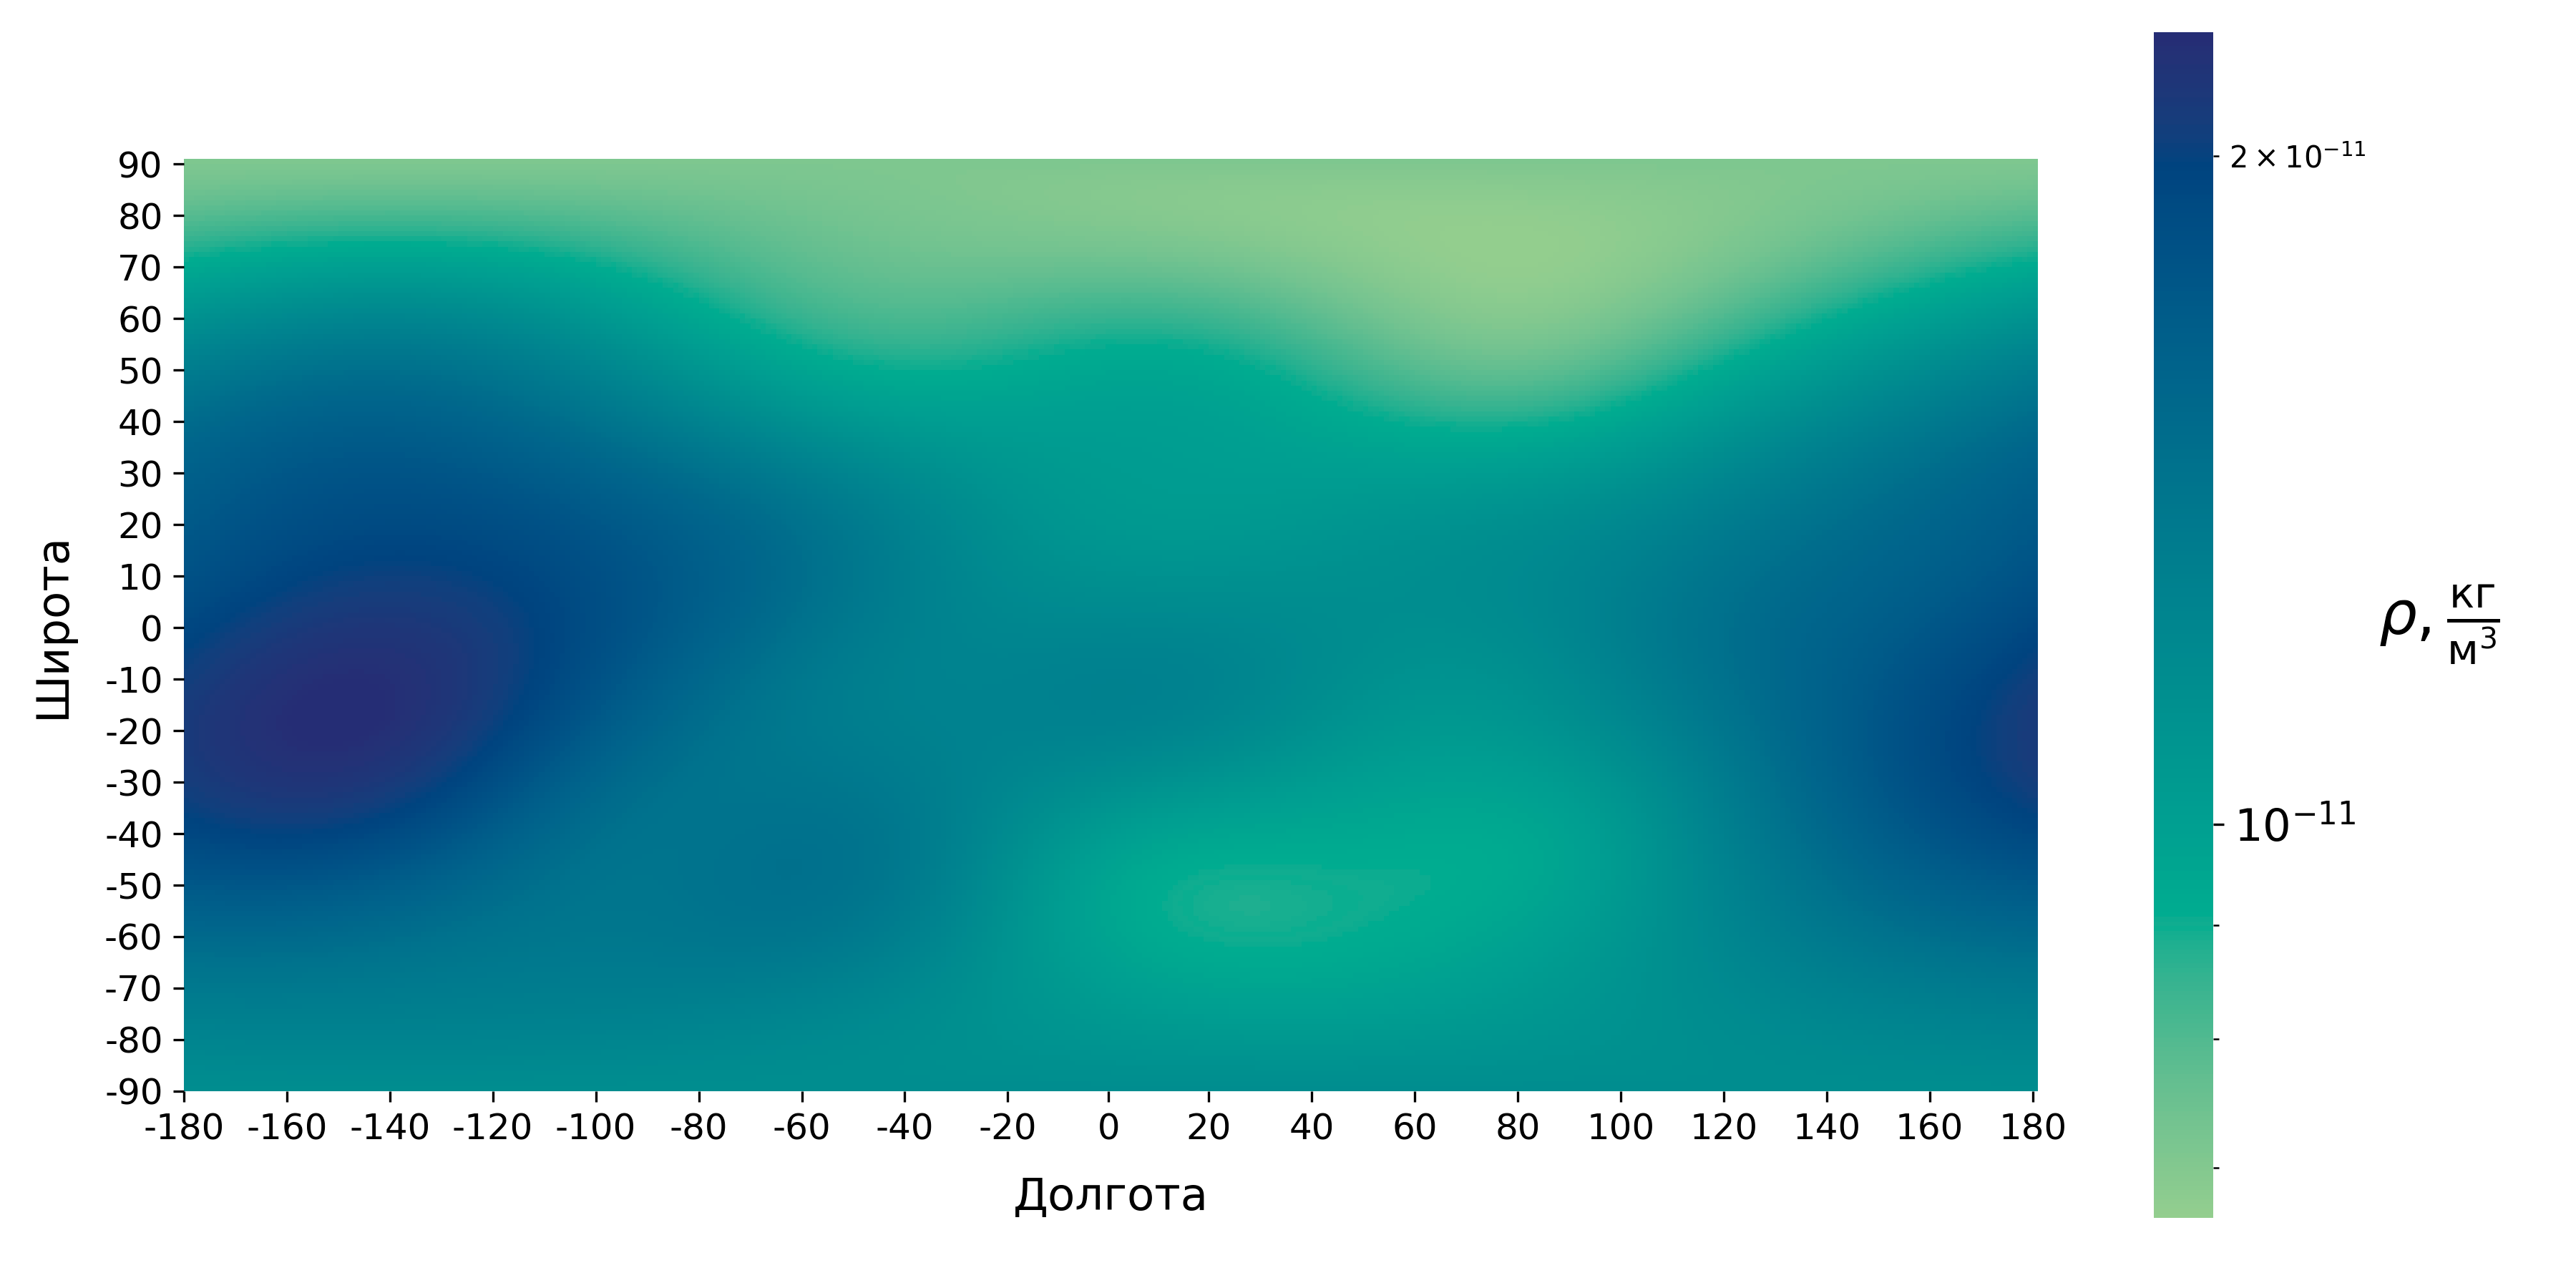
\includegraphics[width=\linewidth]{../images/solution/atmo/2753_latlon_direct_val_heatmap.png}
    \captionof{figure}{Распределение плотности $\rho(\phi, \lambda)$ для конфигурации (2, 7, 5, 3)}
    \label{fig:atmo:2753_latlon}
 \end{figure}

 \begin{figure}[h!]
    \centering
    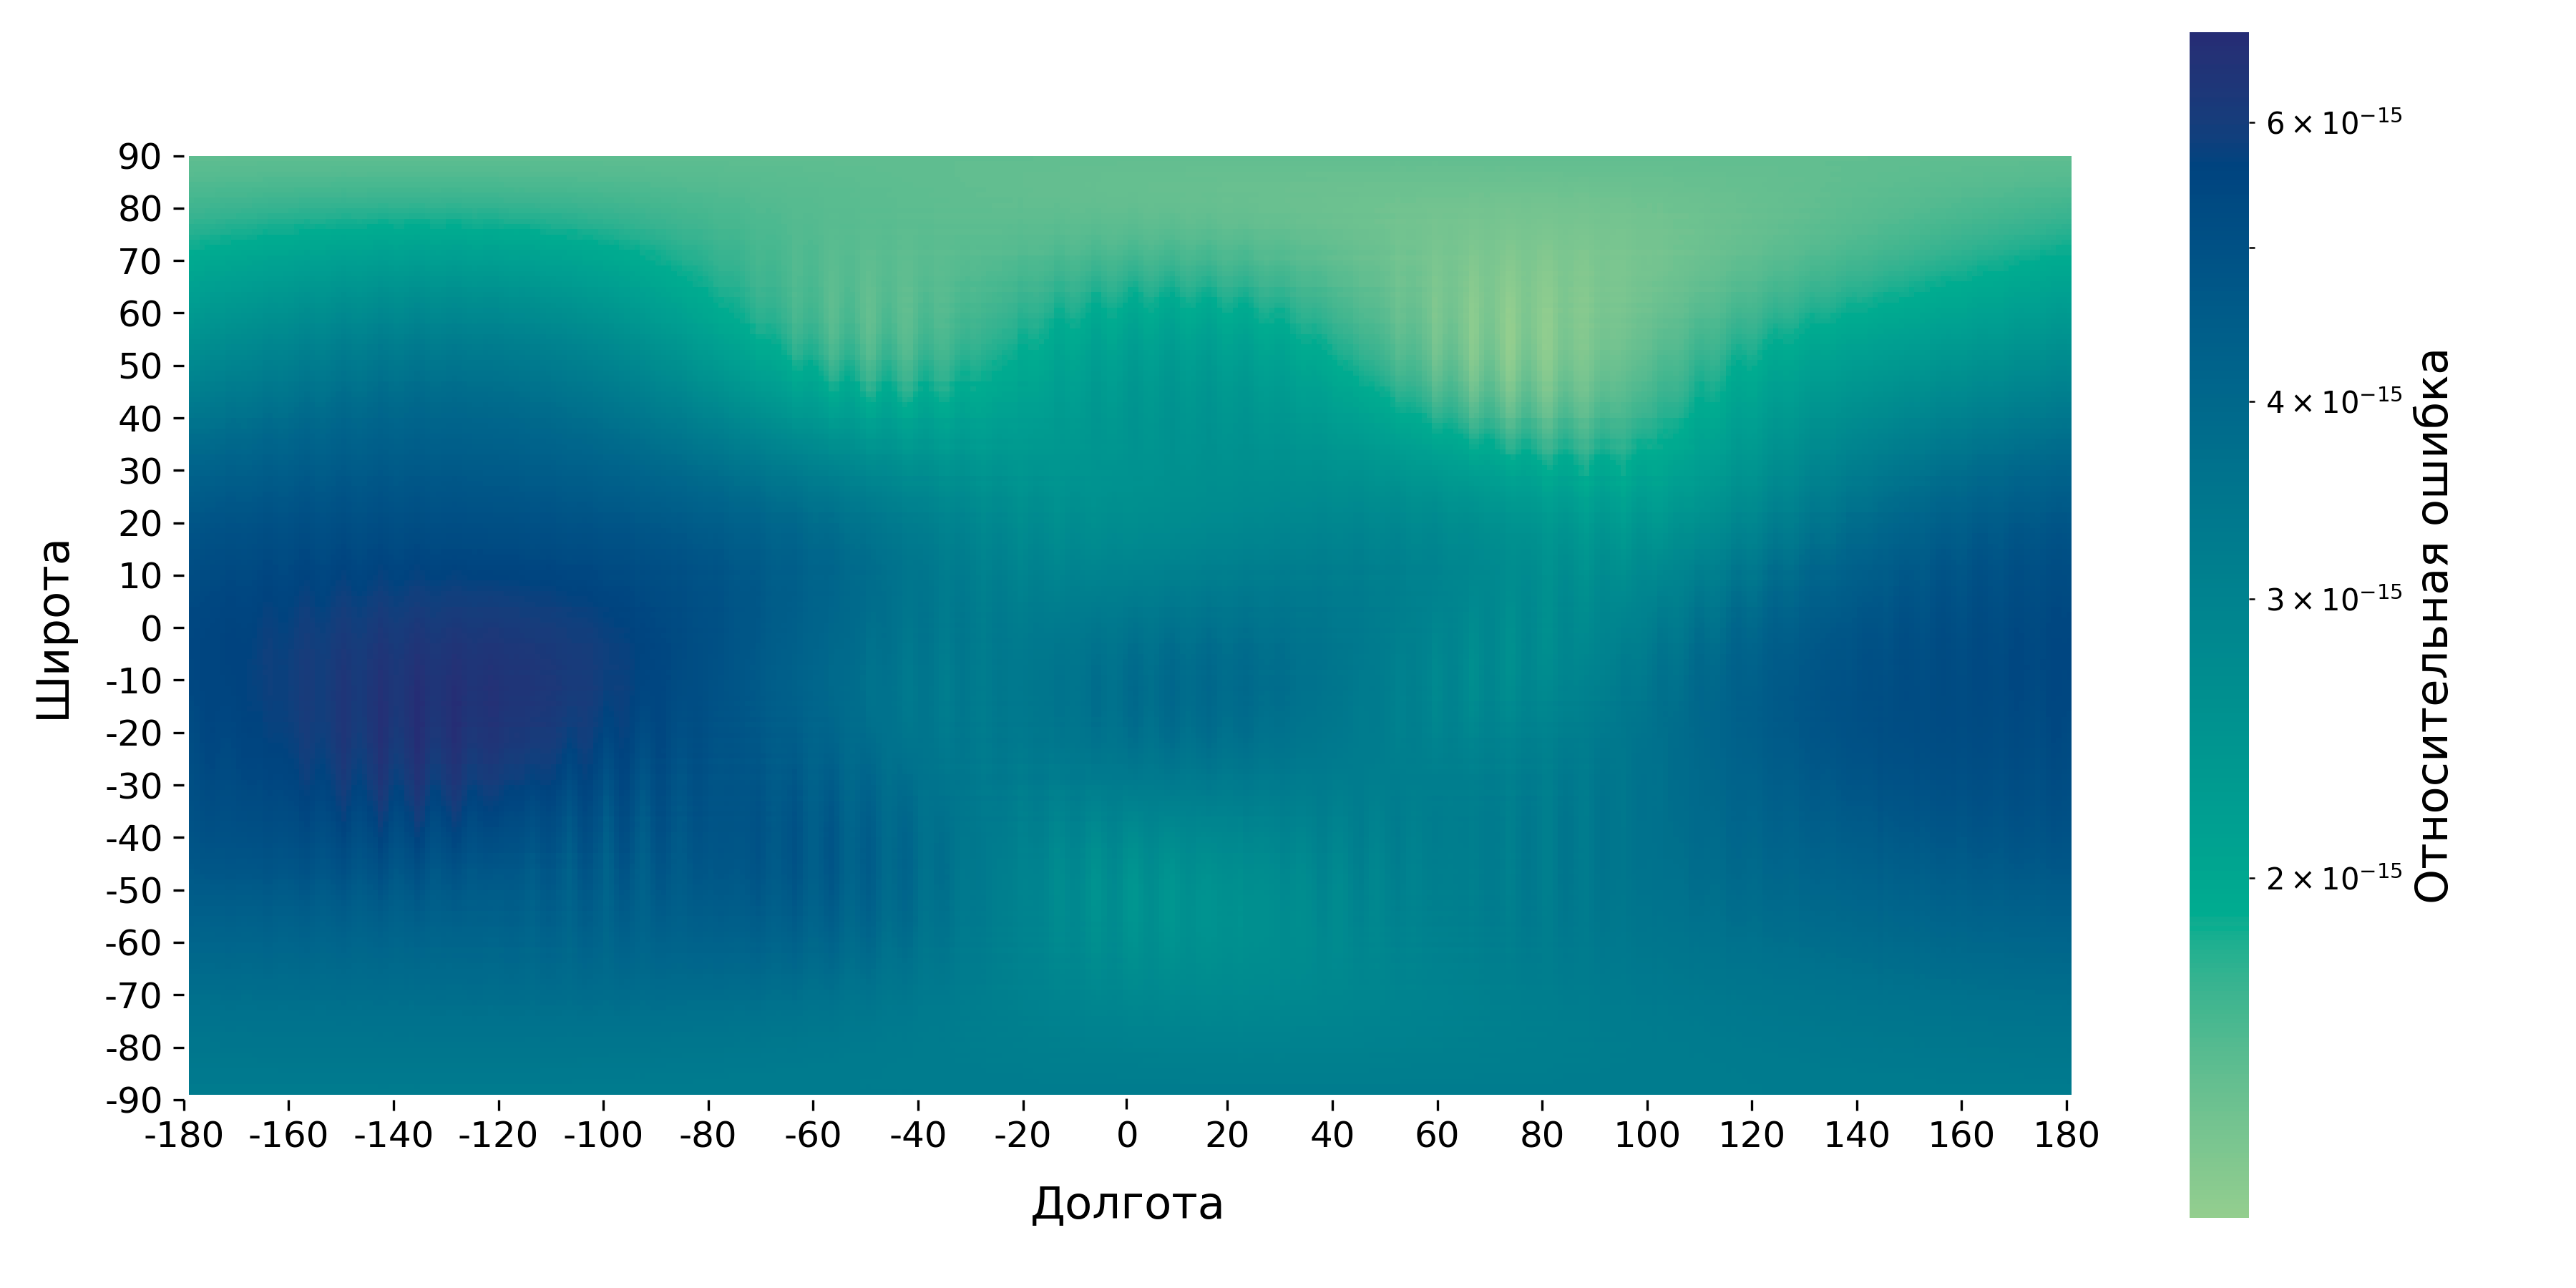
\includegraphics[width=\linewidth]{../images/solution/atmo/2753_latlon_abs_error_heatmap.png}
    \captionof{figure}{Распределение абсолютной ошибки вычисления плотности для конфигурации (2, 7, 5, 3)}
    \label{fig:atmo:2753_latlon_abs_err}
 \end{figure}

 На основе данных о поточечном сравнеии для каждой конфигурации были подобраны интерполянты, 
 позволяющие достичь малой ошибки при минимальном размере. 
 Характеристики выбранных интерполянтов представлены в таблице \ref{tab:atmo_propag}.

 Тестирование прогноза с использованием интерполянтов проводилось следующим образом.
 Большая часть космических объектов имеет отношение площади к массе 0.001 -- 0.1,
 поэтому в тестах этот параметр был зафиксирован на величине 0.1. Исходя из дополнительных
 рассчетов, зависимость ошибки прогноза от данного параметра близка к линейной. Поэтому
 ошибку для объектов с большим соотношением площади к массе (например, у пленок) 
 можно легко получить.
 Рассмотрено более 5000 тысяч околоземных орбит с высотами от 350 до 800 километров. 
 Гравитация учитывалась по модели EGM2008 с 64 гармониками. Вычисления проводились
 с помощью явного метода Рунге--Кутты 7-го порядка, а период интегрирования составил 1 день.
 Сначала траектория вычислялась напрямую, затем с интерполяцией плотности атмосферы.
 За ошибку принята разность между двумя прогнозами. Для наглядности на рисунках 
 \ref{fig:atmo:2357_propag_1} -- \ref{fig:atmo:2735_propag}
 приведена максимальная ошибка по высотам орбит с интервалом 50--100 км.

 На исследованных интерполянтах ошибки в пределах 10 метра удается достичь на высотах
 от 400 километров. Такую точность можно считать достаточной при построении НОО.

 Как отмечалось ранее, ускорение интерполянта главным образом зависит от скорости
 вычисления линейной комбинации произведений полиномов Чебышева в ячейке. 
 Эта скорость определяется максимальным порядком каждого полинома. Поэтому каждая
 рассмотренная конфигурация дает примерно одно и то же ускорение. Небольшие различия
 могут быть вызваны объемом интерполянта. Коэффициенты интерполяции во время исполнения
 программы хранятся в оперативной памяти. Эффективность работы памяти, 
 т. е. скорость доступа к ее участку, уменьшается на больших данных. В то же время
 такое замедление не критично, так как качественно не меняет степень ускорения.

 Скорость вычисления плотности атмосферы с интерполянтом выросла в среднем в 17 раз.
 Минимальное ускорение достигалось на больших интерполянтах и равнялось 9. Для избранных
 интерполянтов ускорение варьировалось от 13 до 14. Таким образом, был достигнут
 уровень ресурсоемкости вычисления гравитационного потенциала с интерполяцией.

 \begin{table}[h!]
    \centering
    \renewcommand{\arraystretch}{1.5}
    \begin{tabular}{|c|c|c|c|c|}
    \hline
    Конфигурация & Количество ячеек & \begin{tabular}[c]{@{}c@{}}Относительная \\ ошибка, \%\end{tabular} & \begin{tabular}[c]{@{}c@{}}Максимальная \\ ошибка прогноза, м\end{tabular} & Размер, ГБ \\ \hline
    (2, 3, 5, 7) & (65, 50, 25, 20) & 0.045                                                               & 12.2                                                                       & 0.97       \\ \hline
    (2, 3, 5, 7) & (65, 45, 35, 20) & 0.041                                                               & 12.3                                                                       & 1.22       \\ \hline
    (2, 3, 7, 5) & (65, 45, 15, 35) & 0.044                                                               & 11.8                                                                       & 0.91       \\ \hline
    (2, 5, 3, 7) & (65, 25, 50, 20) & 0.044                                                               & 12.3                                                                       & 0.97       \\ \hline
    (2, 5, 7, 3) & (65, 25, 20, 50) & 0.042                                                               & 12.6                                                                       & 0.97       \\ \hline
    (2, 7, 3, 5) & (65, 15, 45, 40) & 0.044                                                            & 12.2                                                                       & 1.05       \\ \hline
    \end{tabular}
    \caption{Результаты тестирования выбранных интерполянтов}
    \label{tab:atmo_propag}   
\end{table}

\begin{figure}[htbp]
    \centering
    
    % Первая строка
    \begin{subfigure}[b]{0.48\textwidth}
        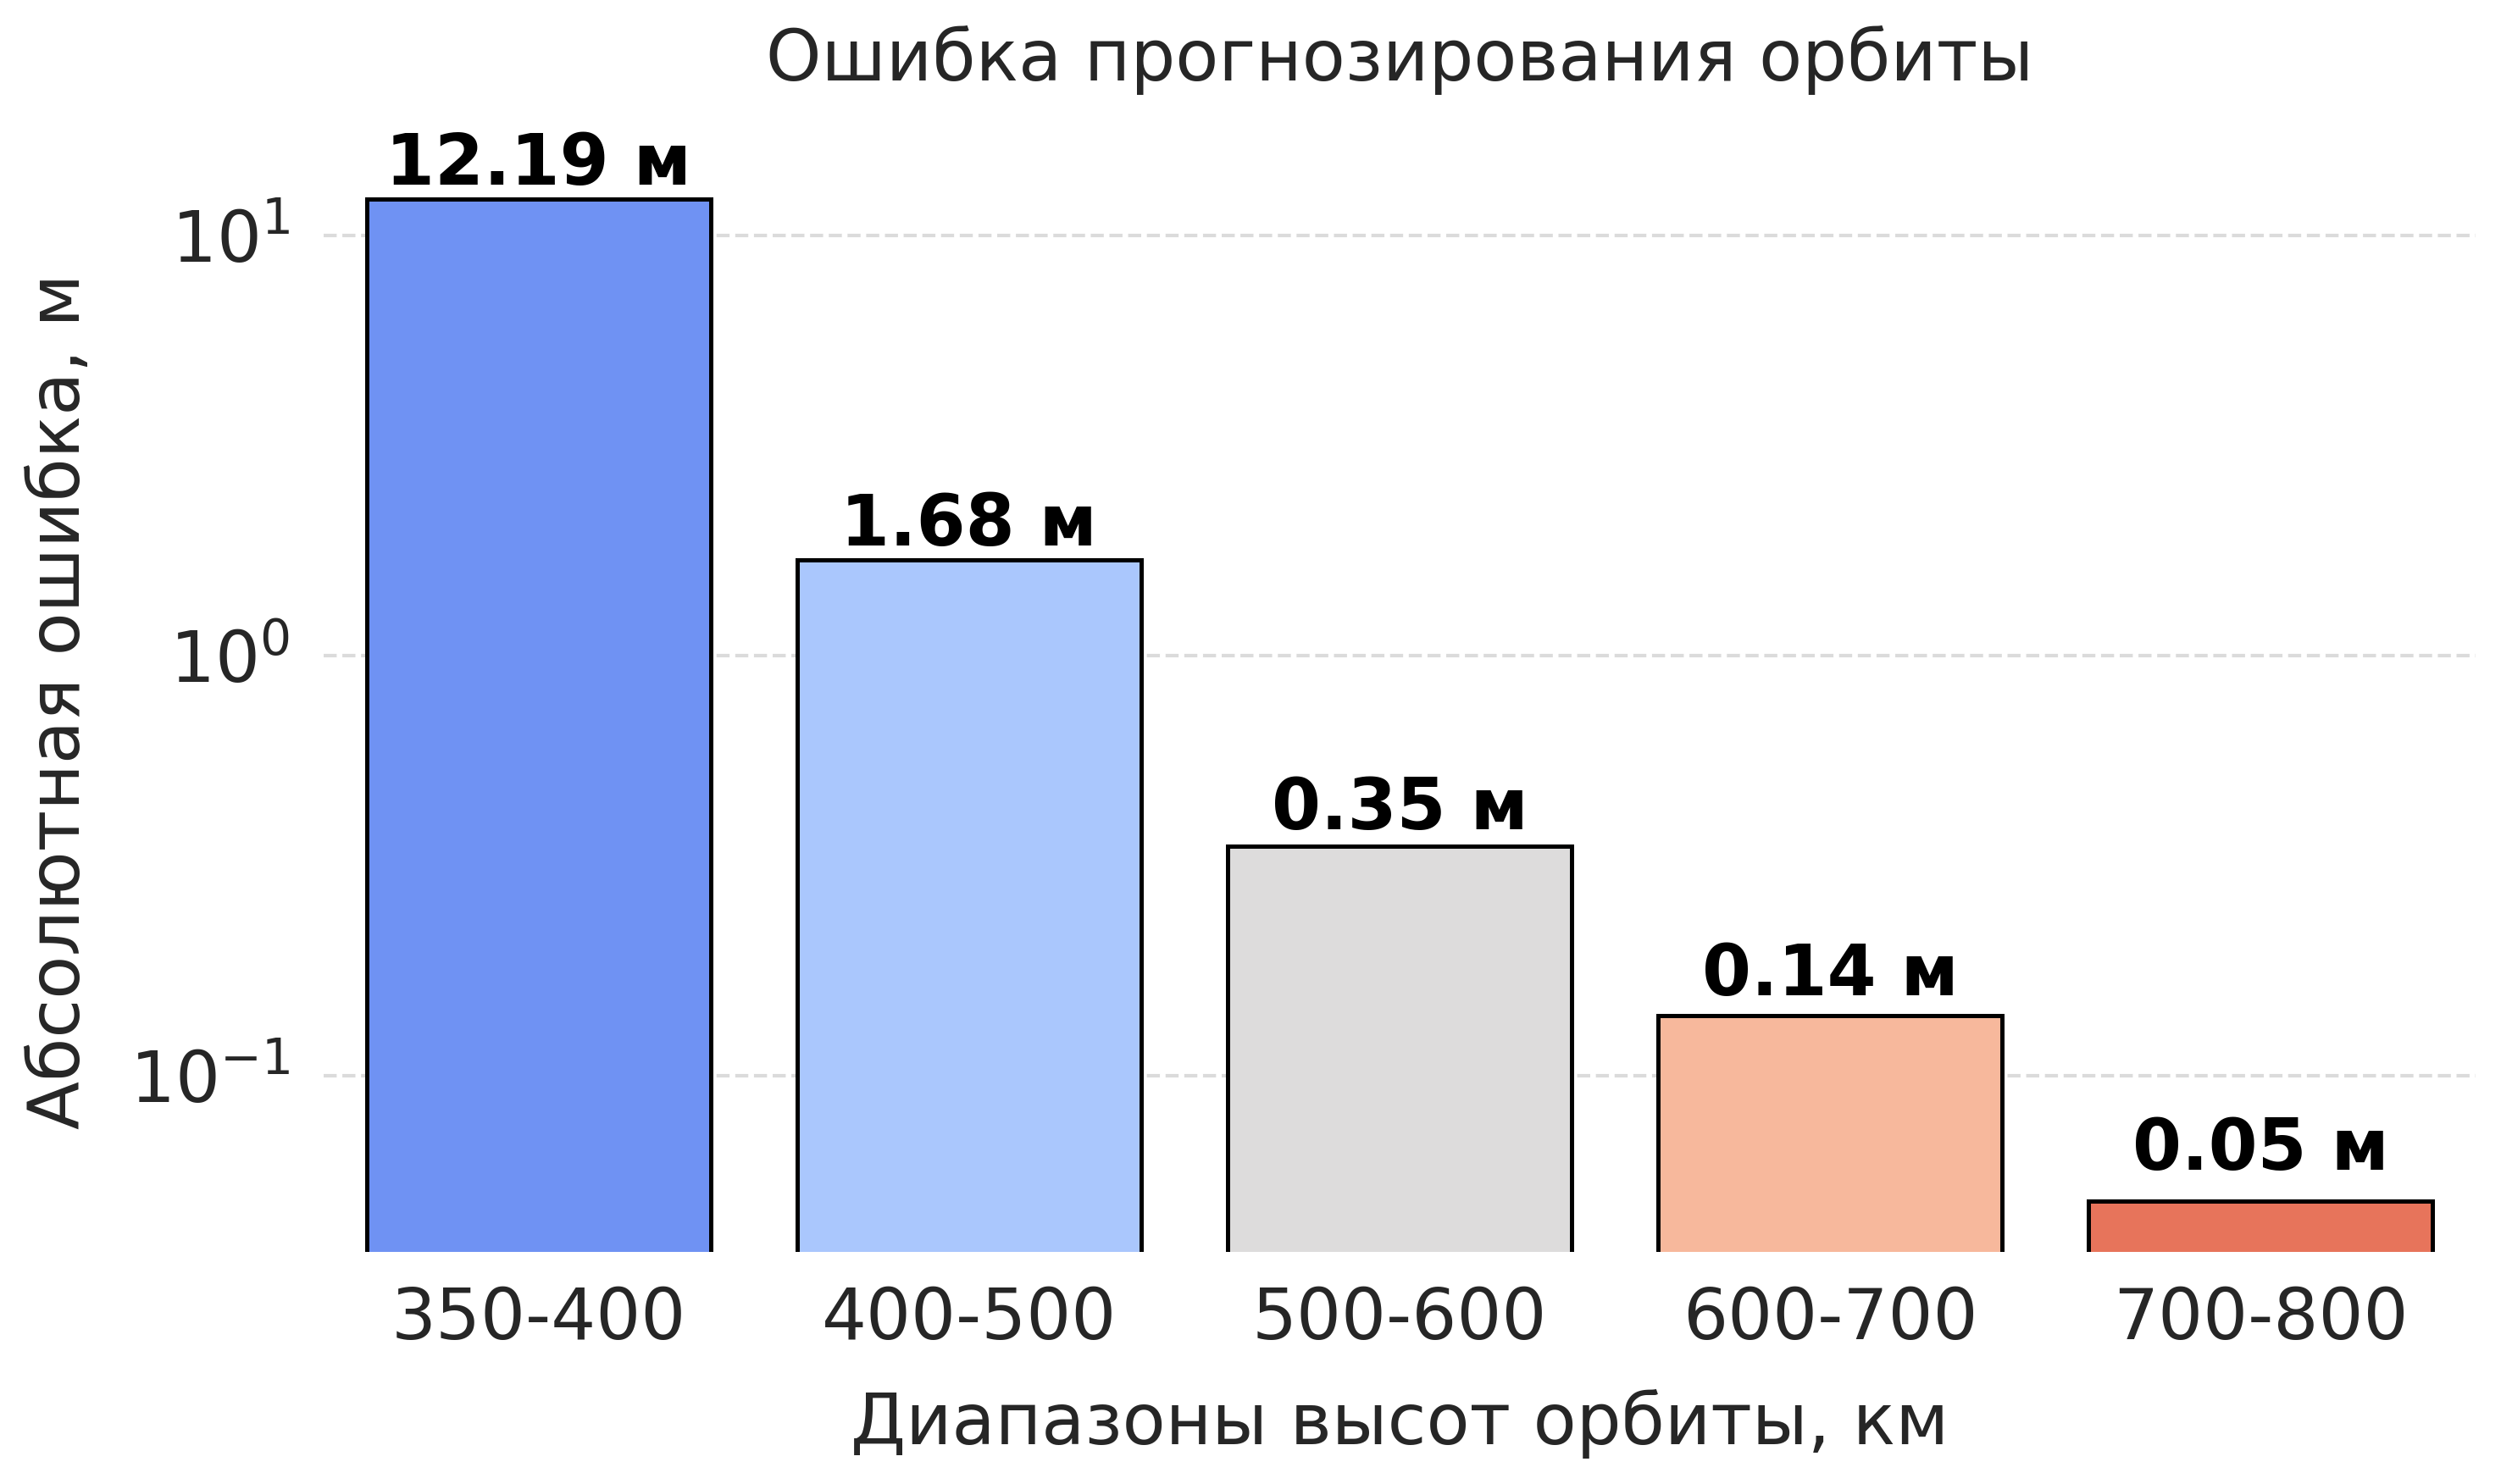
\includegraphics[width=\linewidth]{../images/solution/atmo/propagation/2357_1.png}
        \caption{Конфигурация (2, 3, 5, 7),
        количество ячеек (65, 50, 25, 20)}
        \label{fig:atmo:2357_propag_1}
    \end{subfigure}
    \hfill
    \begin{subfigure}[b]{0.48\textwidth}
        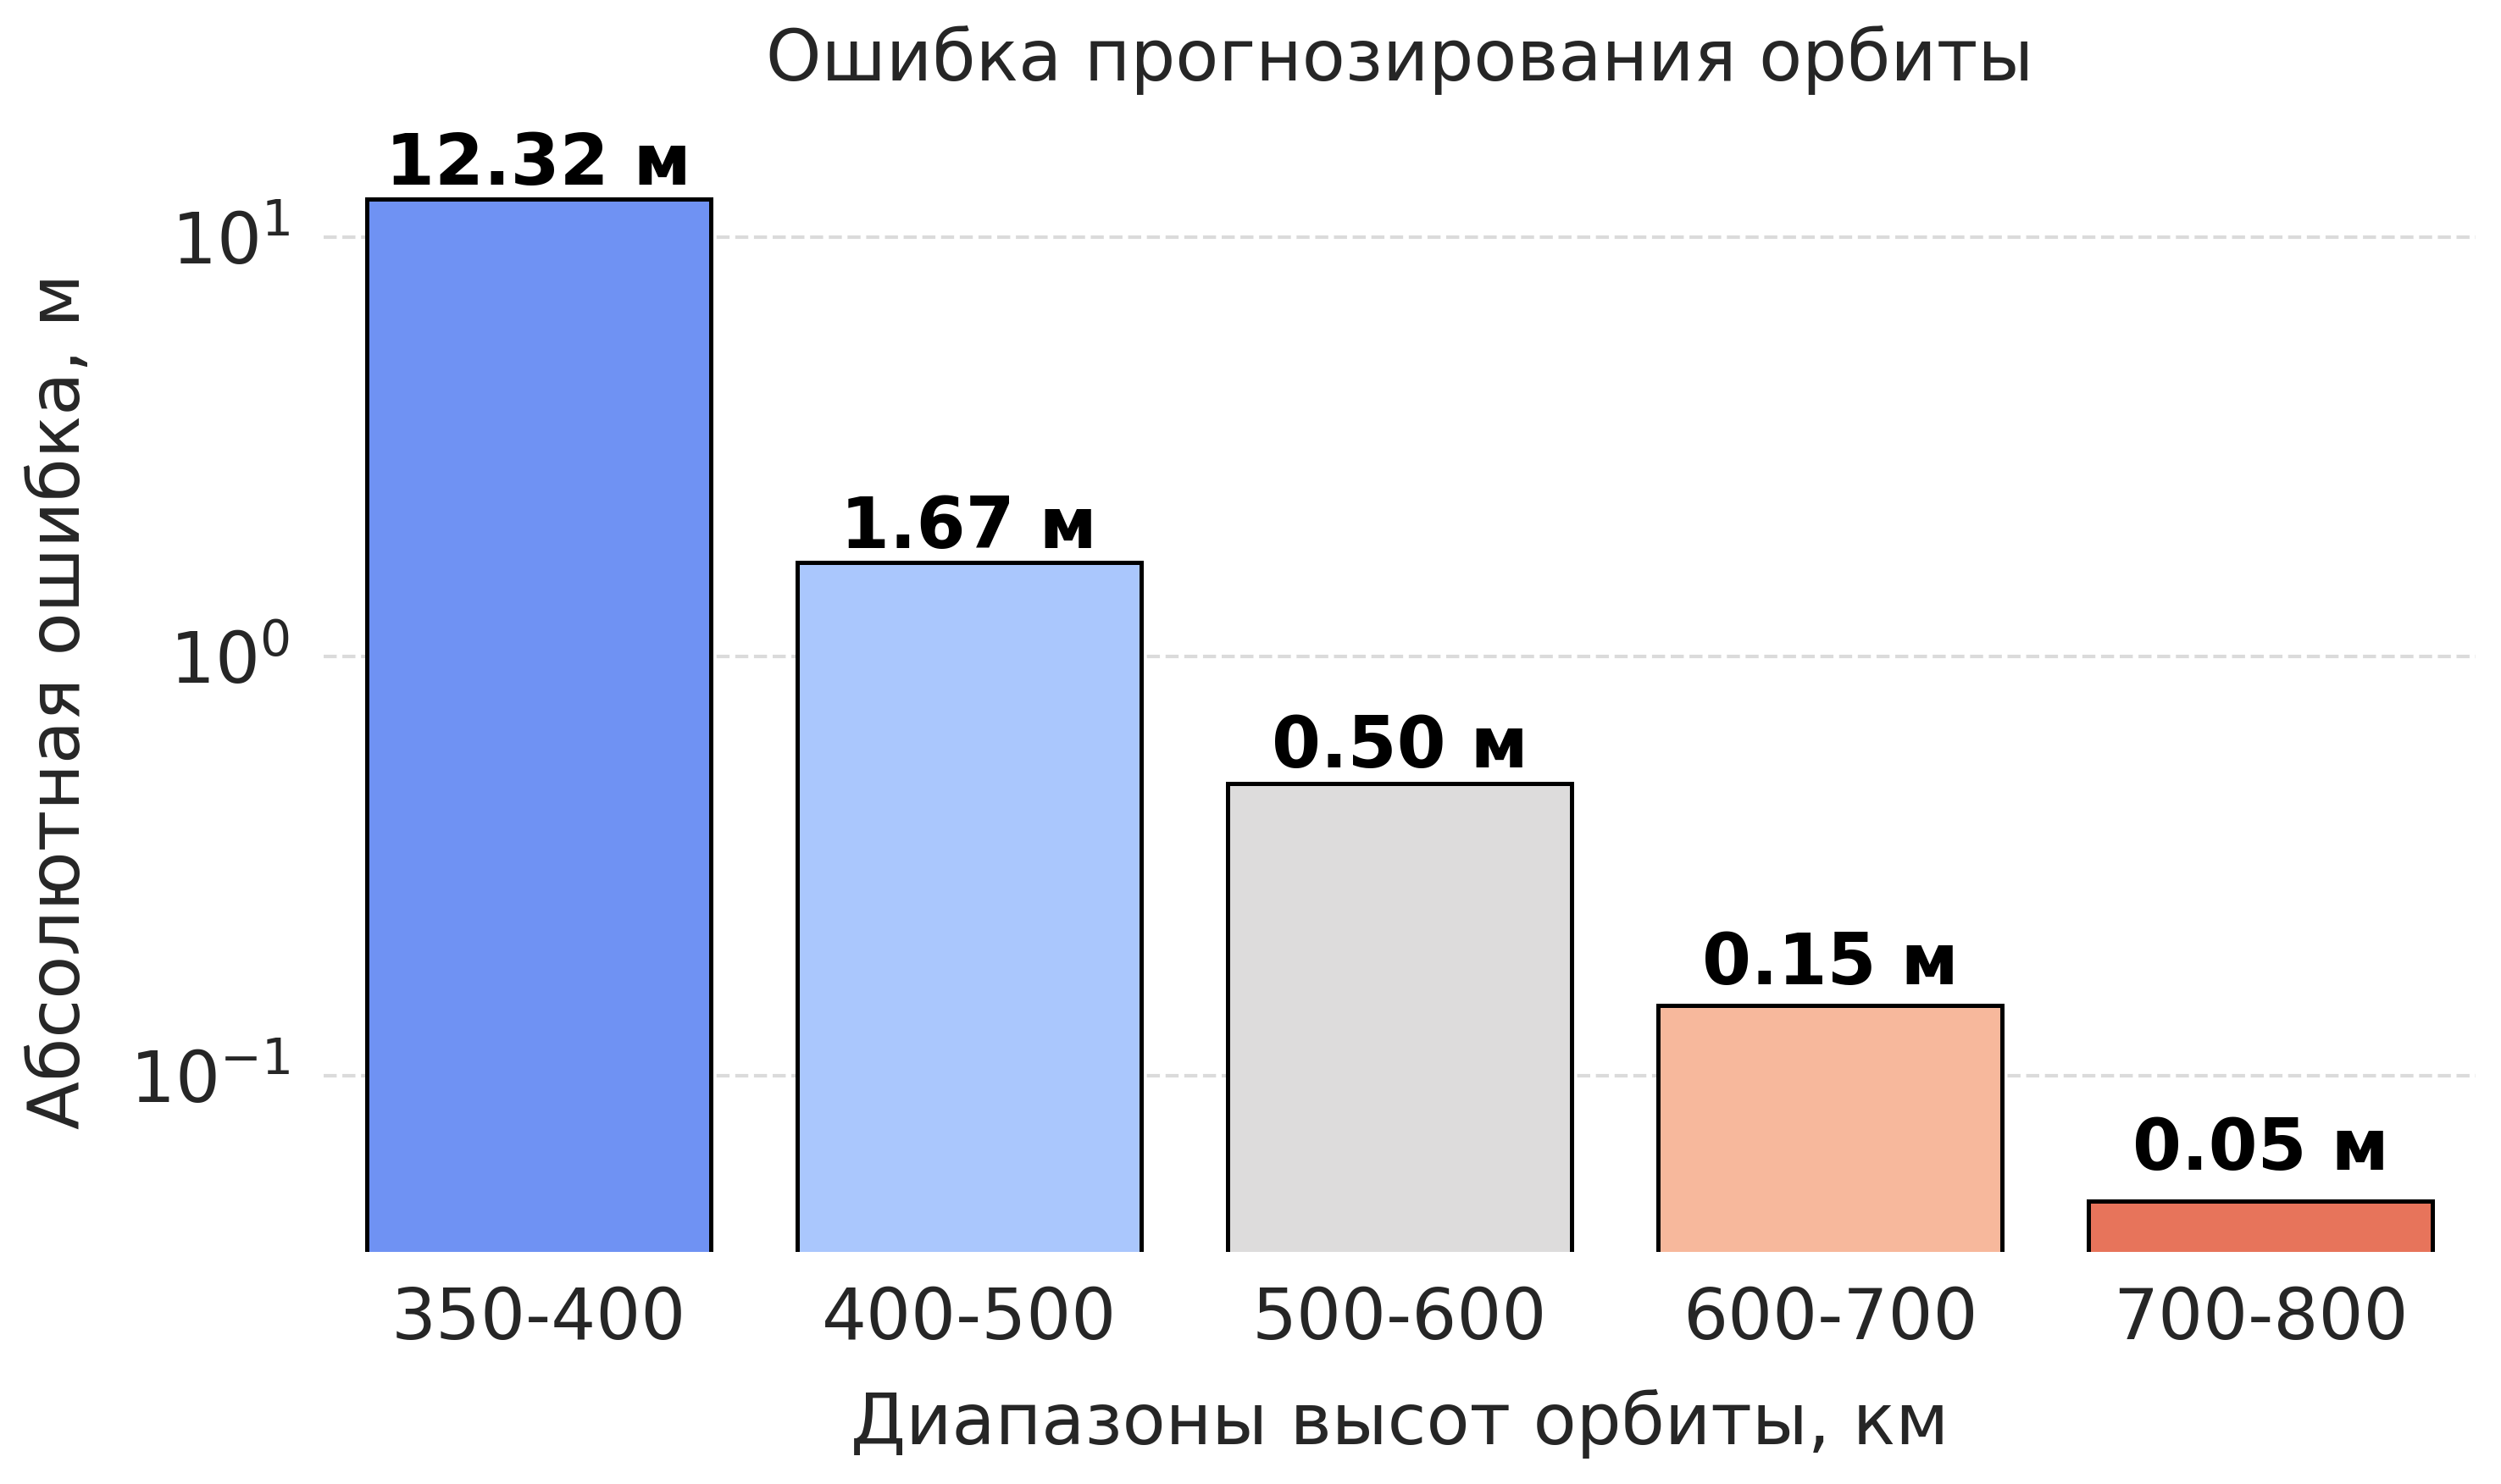
\includegraphics[width=\linewidth]{../images/solution/atmo/propagation/2357_2.png}
        \caption{Конфигурация (2, 3, 5, 7),
        количество ячеек (65, 45, 35, 20)}
        \label{fig:atmo:2357_propag_2}
    \end{subfigure}
    
    \vspace{0.5cm} % Вертикальный отступ между строками
    
    % Вторая строка
    \begin{subfigure}[b]{0.48\textwidth}
        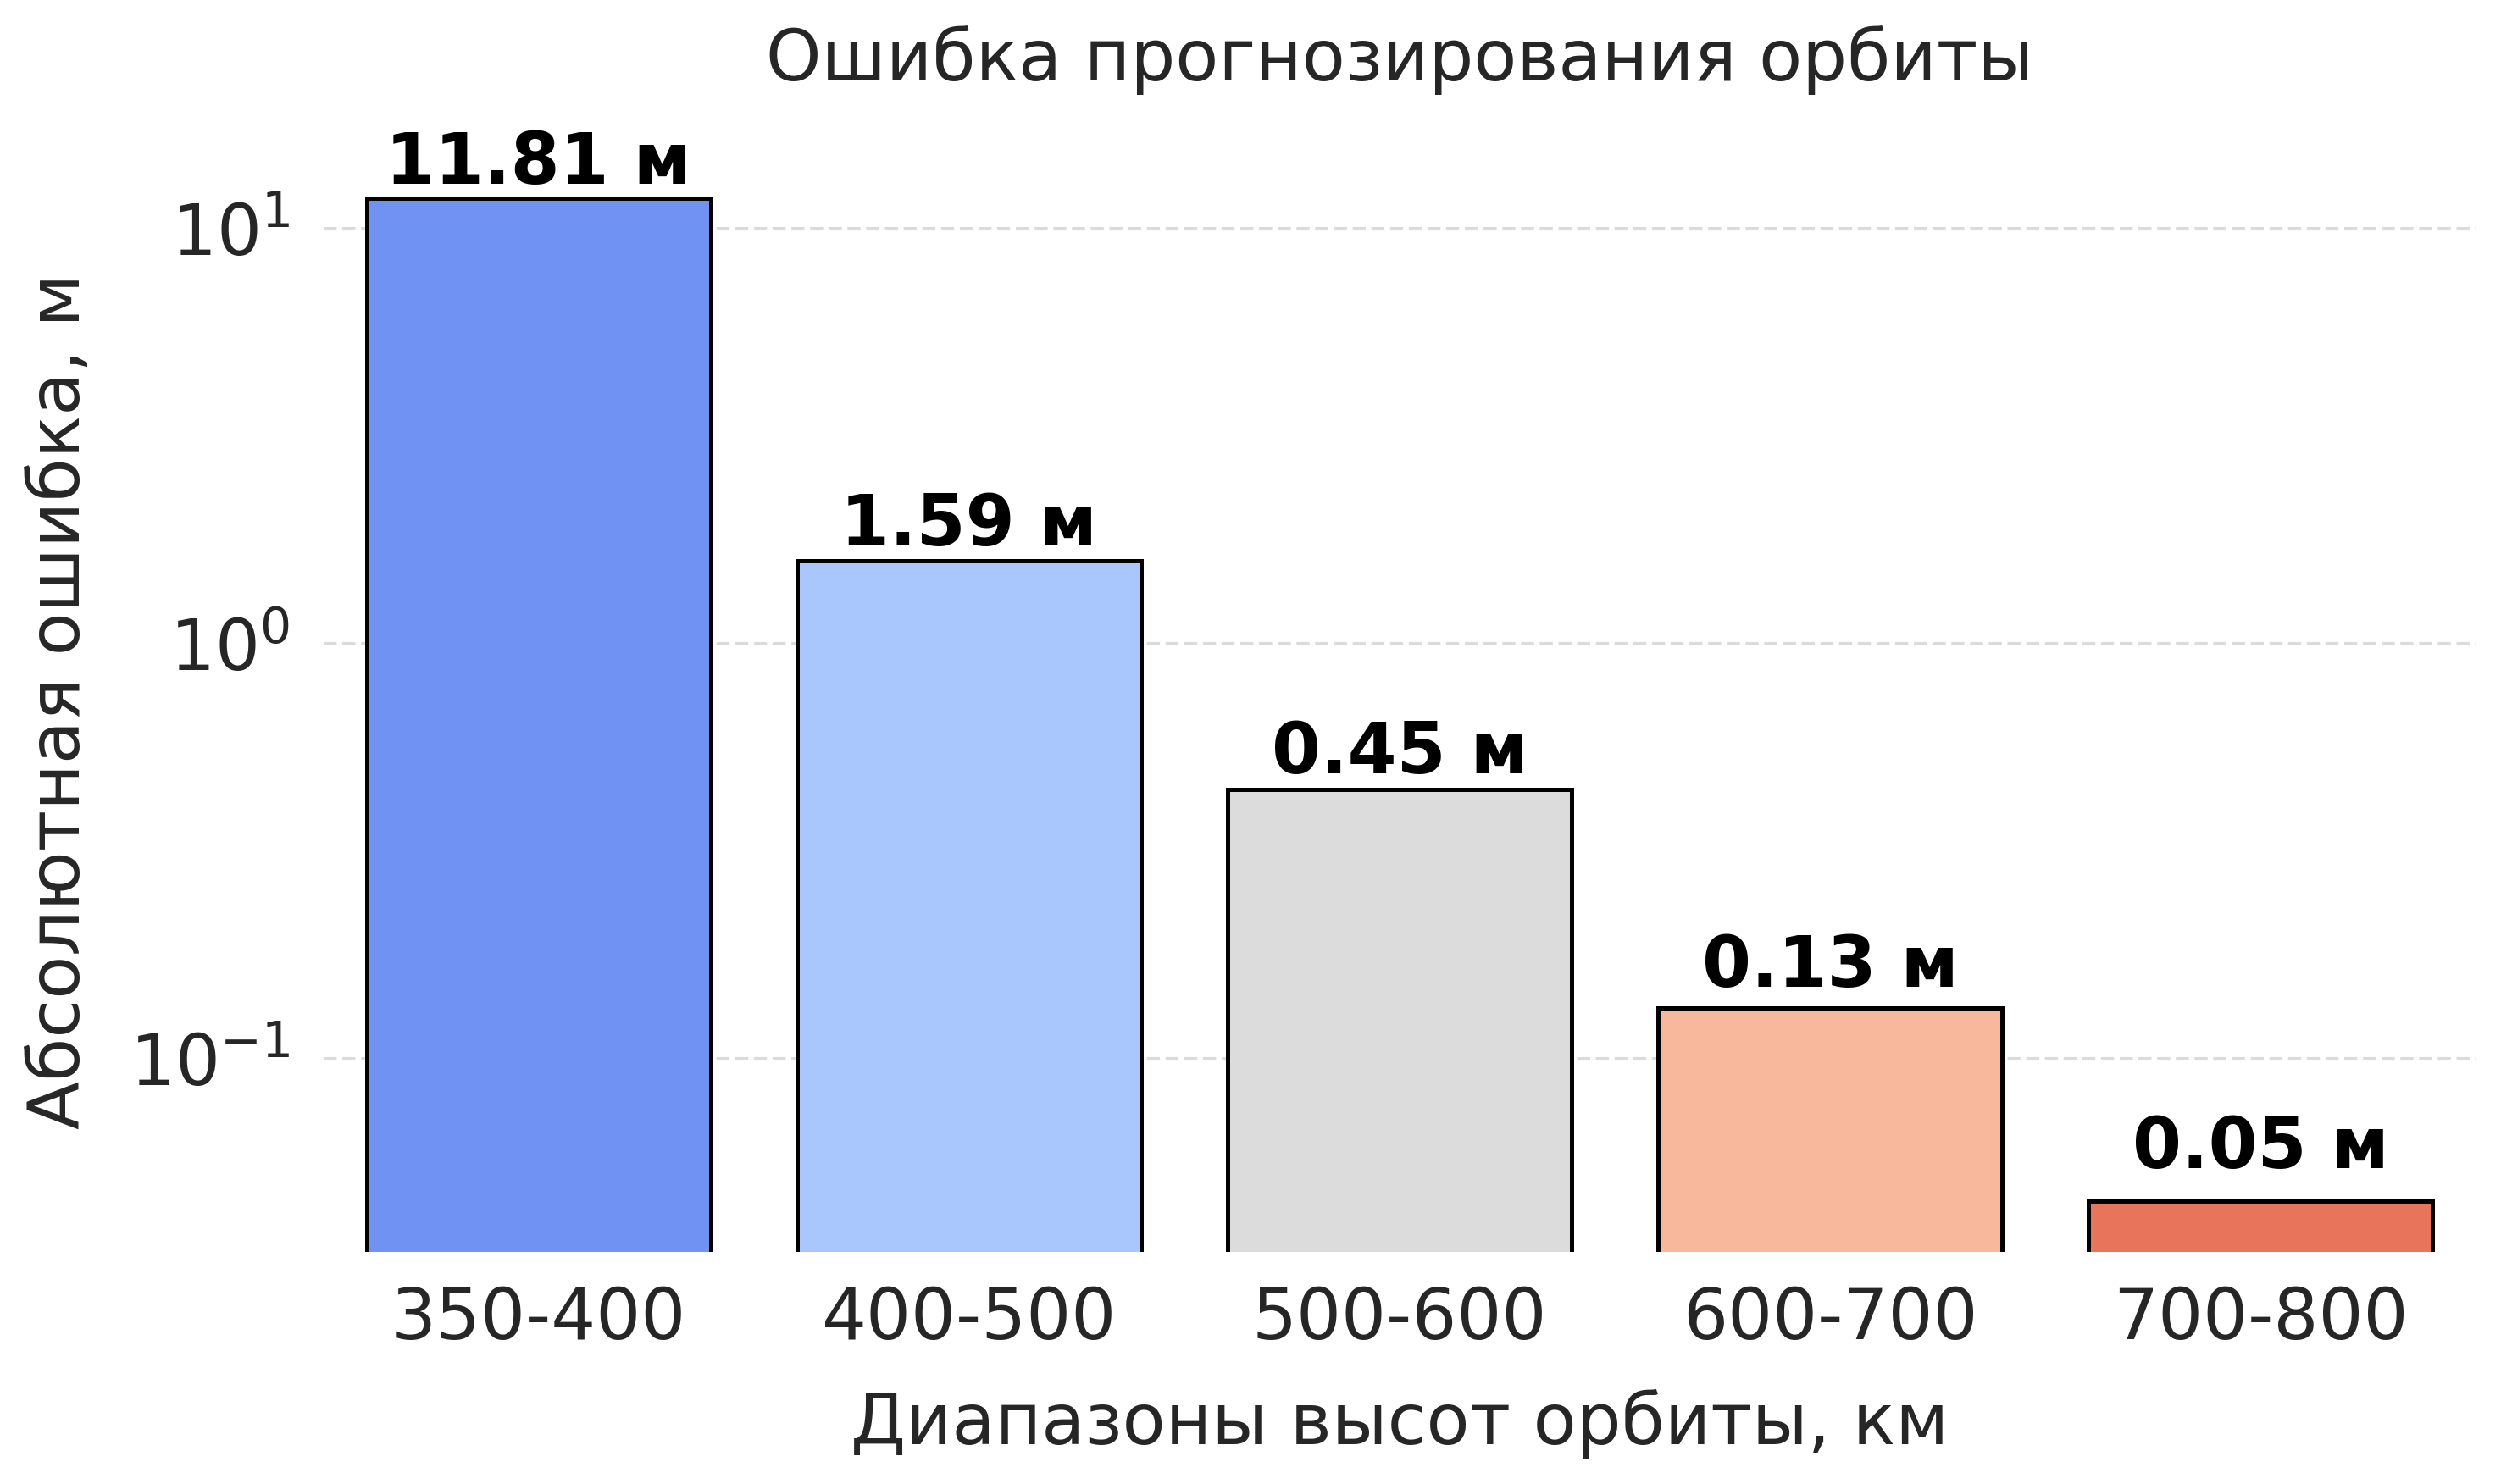
\includegraphics[width=\linewidth]{../images/solution/atmo/propagation/2375.png}
        \caption{Конфигурация (2, 3, 7, 5),
        количество ячеек (65, 45, 15, 35)}
        \label{fig:atmo:2375_propag}
    \end{subfigure}
    \hfill
    \begin{subfigure}[b]{0.48\textwidth}
        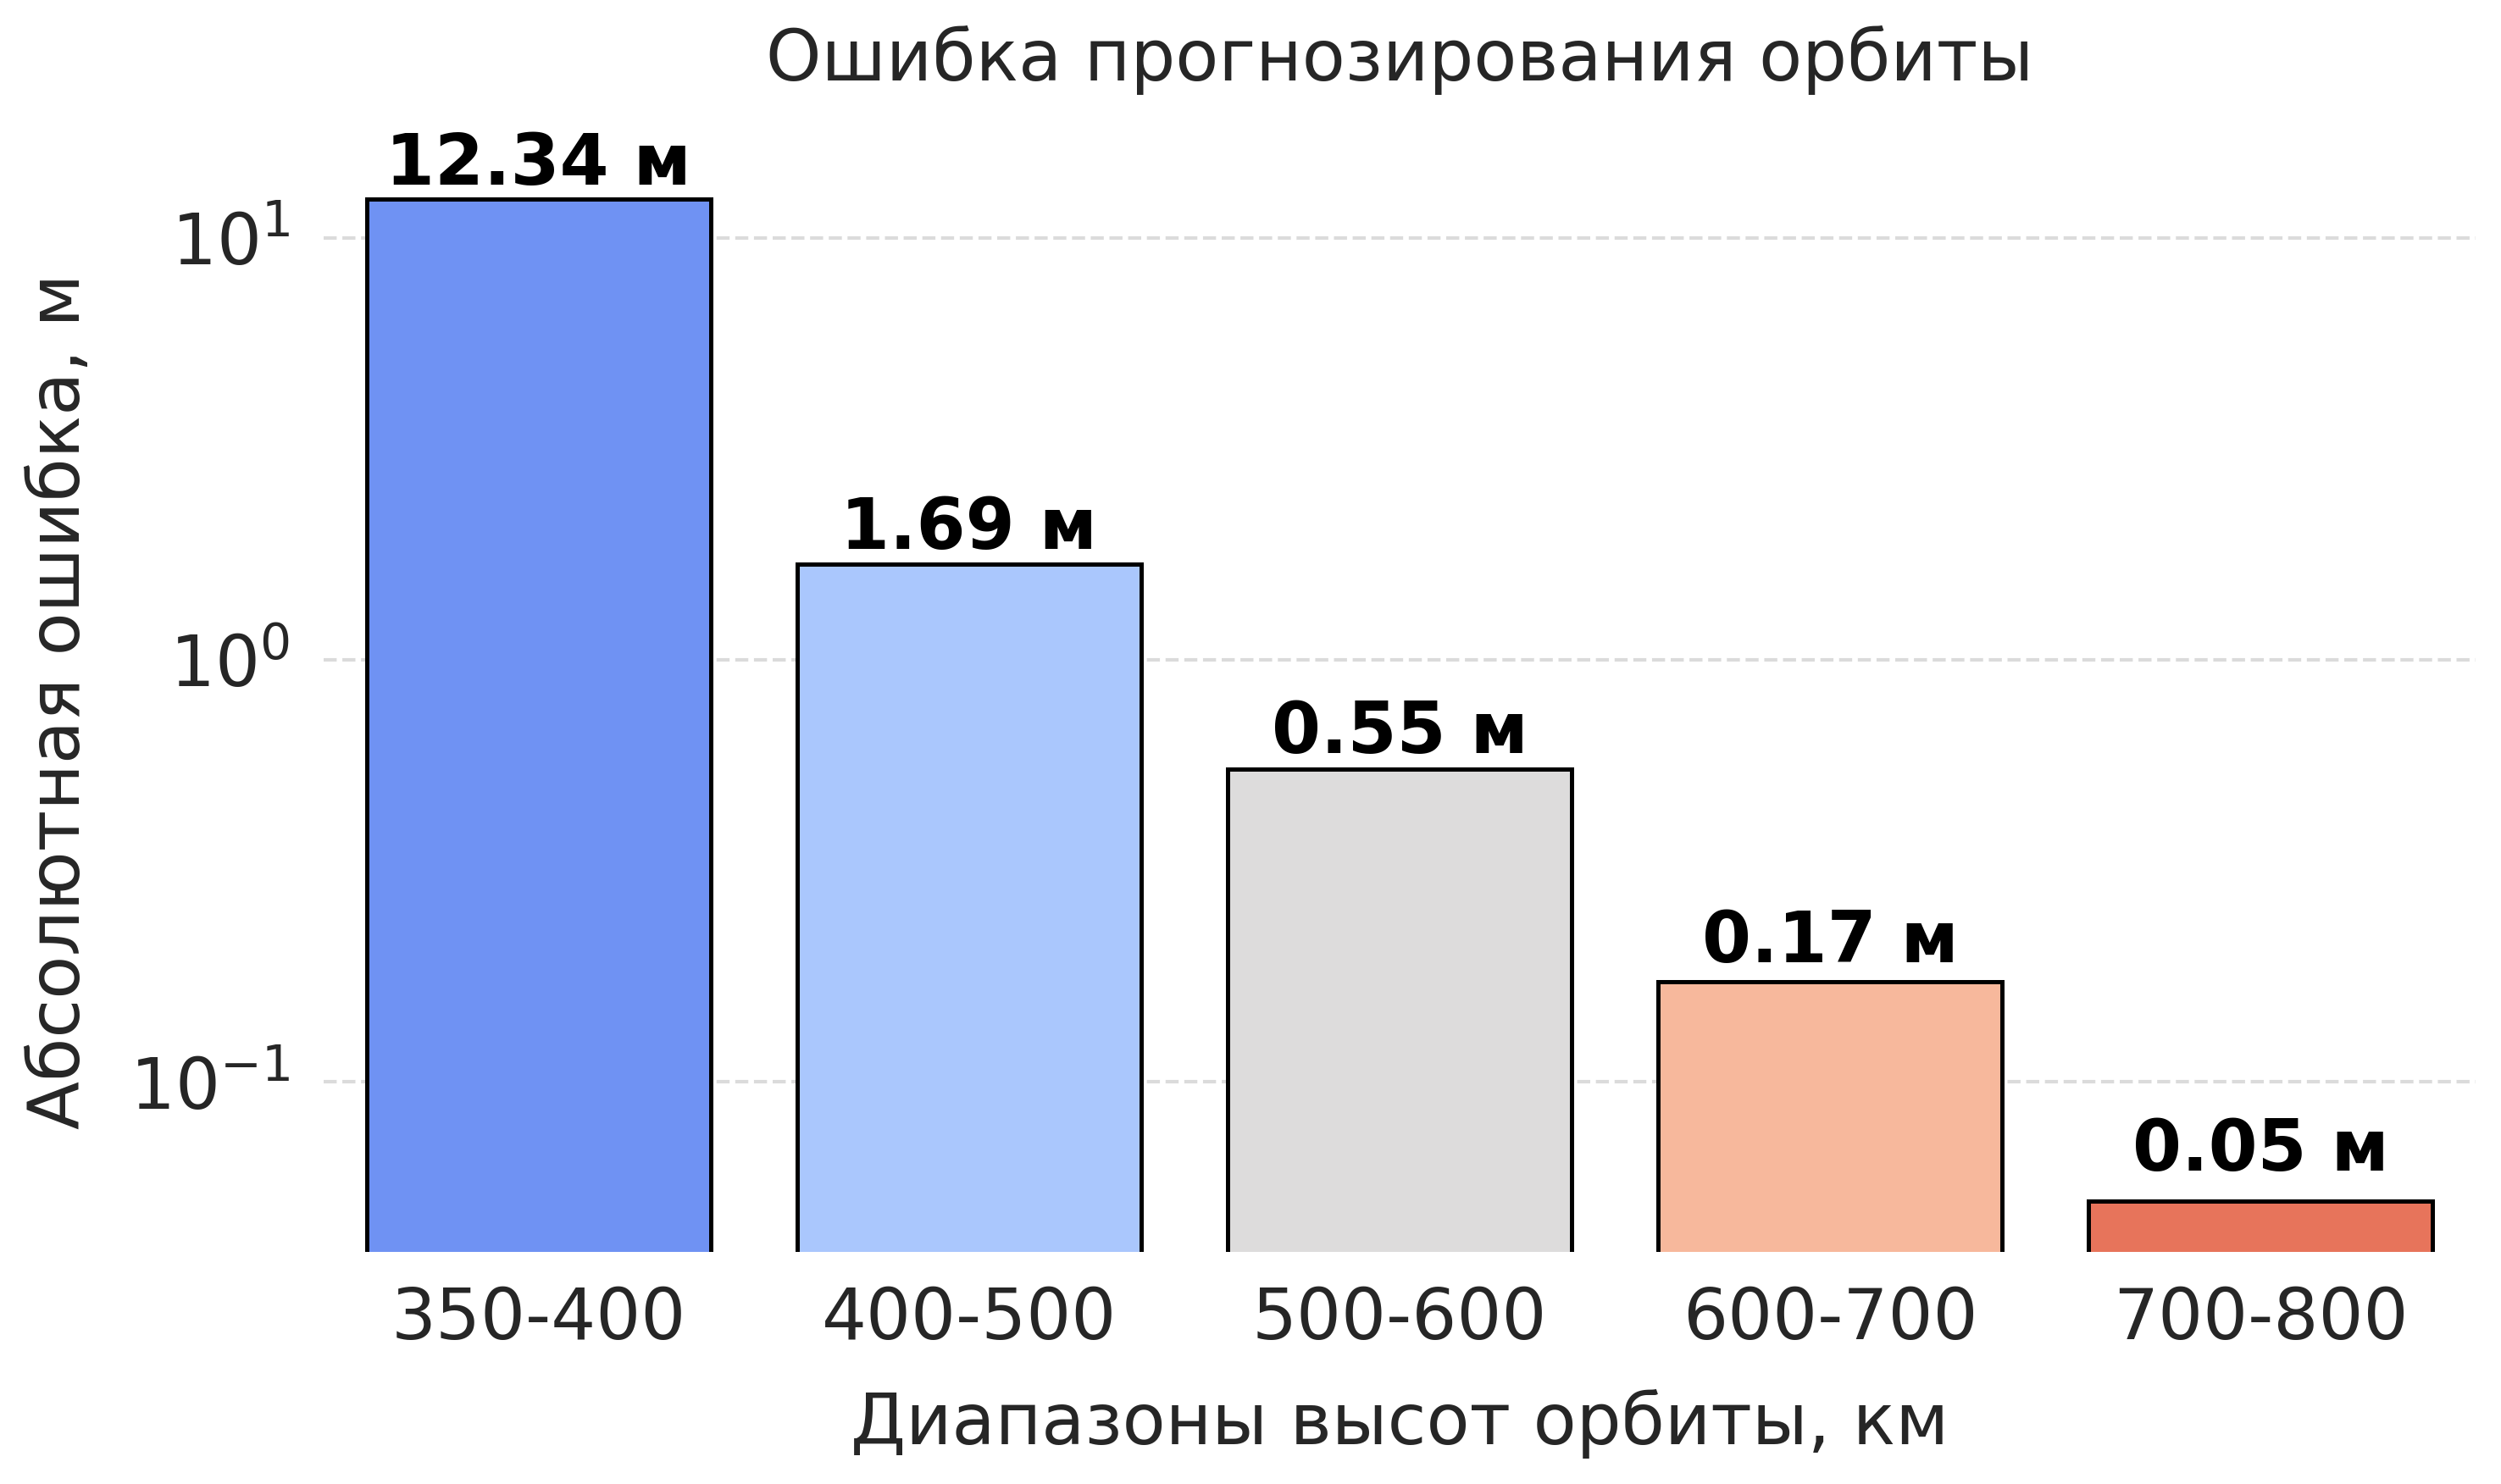
\includegraphics[width=\linewidth]{../images/solution/atmo/propagation/2537.png}
        \caption{Конфигурация (2, 5, 3, 7),
        количество ячеек (65, 25, 50, 20)}
        \label{fig:atmo:2537_propag}
    \end{subfigure}
    
    \vspace{0.5cm} % Вертикальный отступ между строками
    
    % Третья строка
    \begin{subfigure}[b]{0.48\textwidth}
        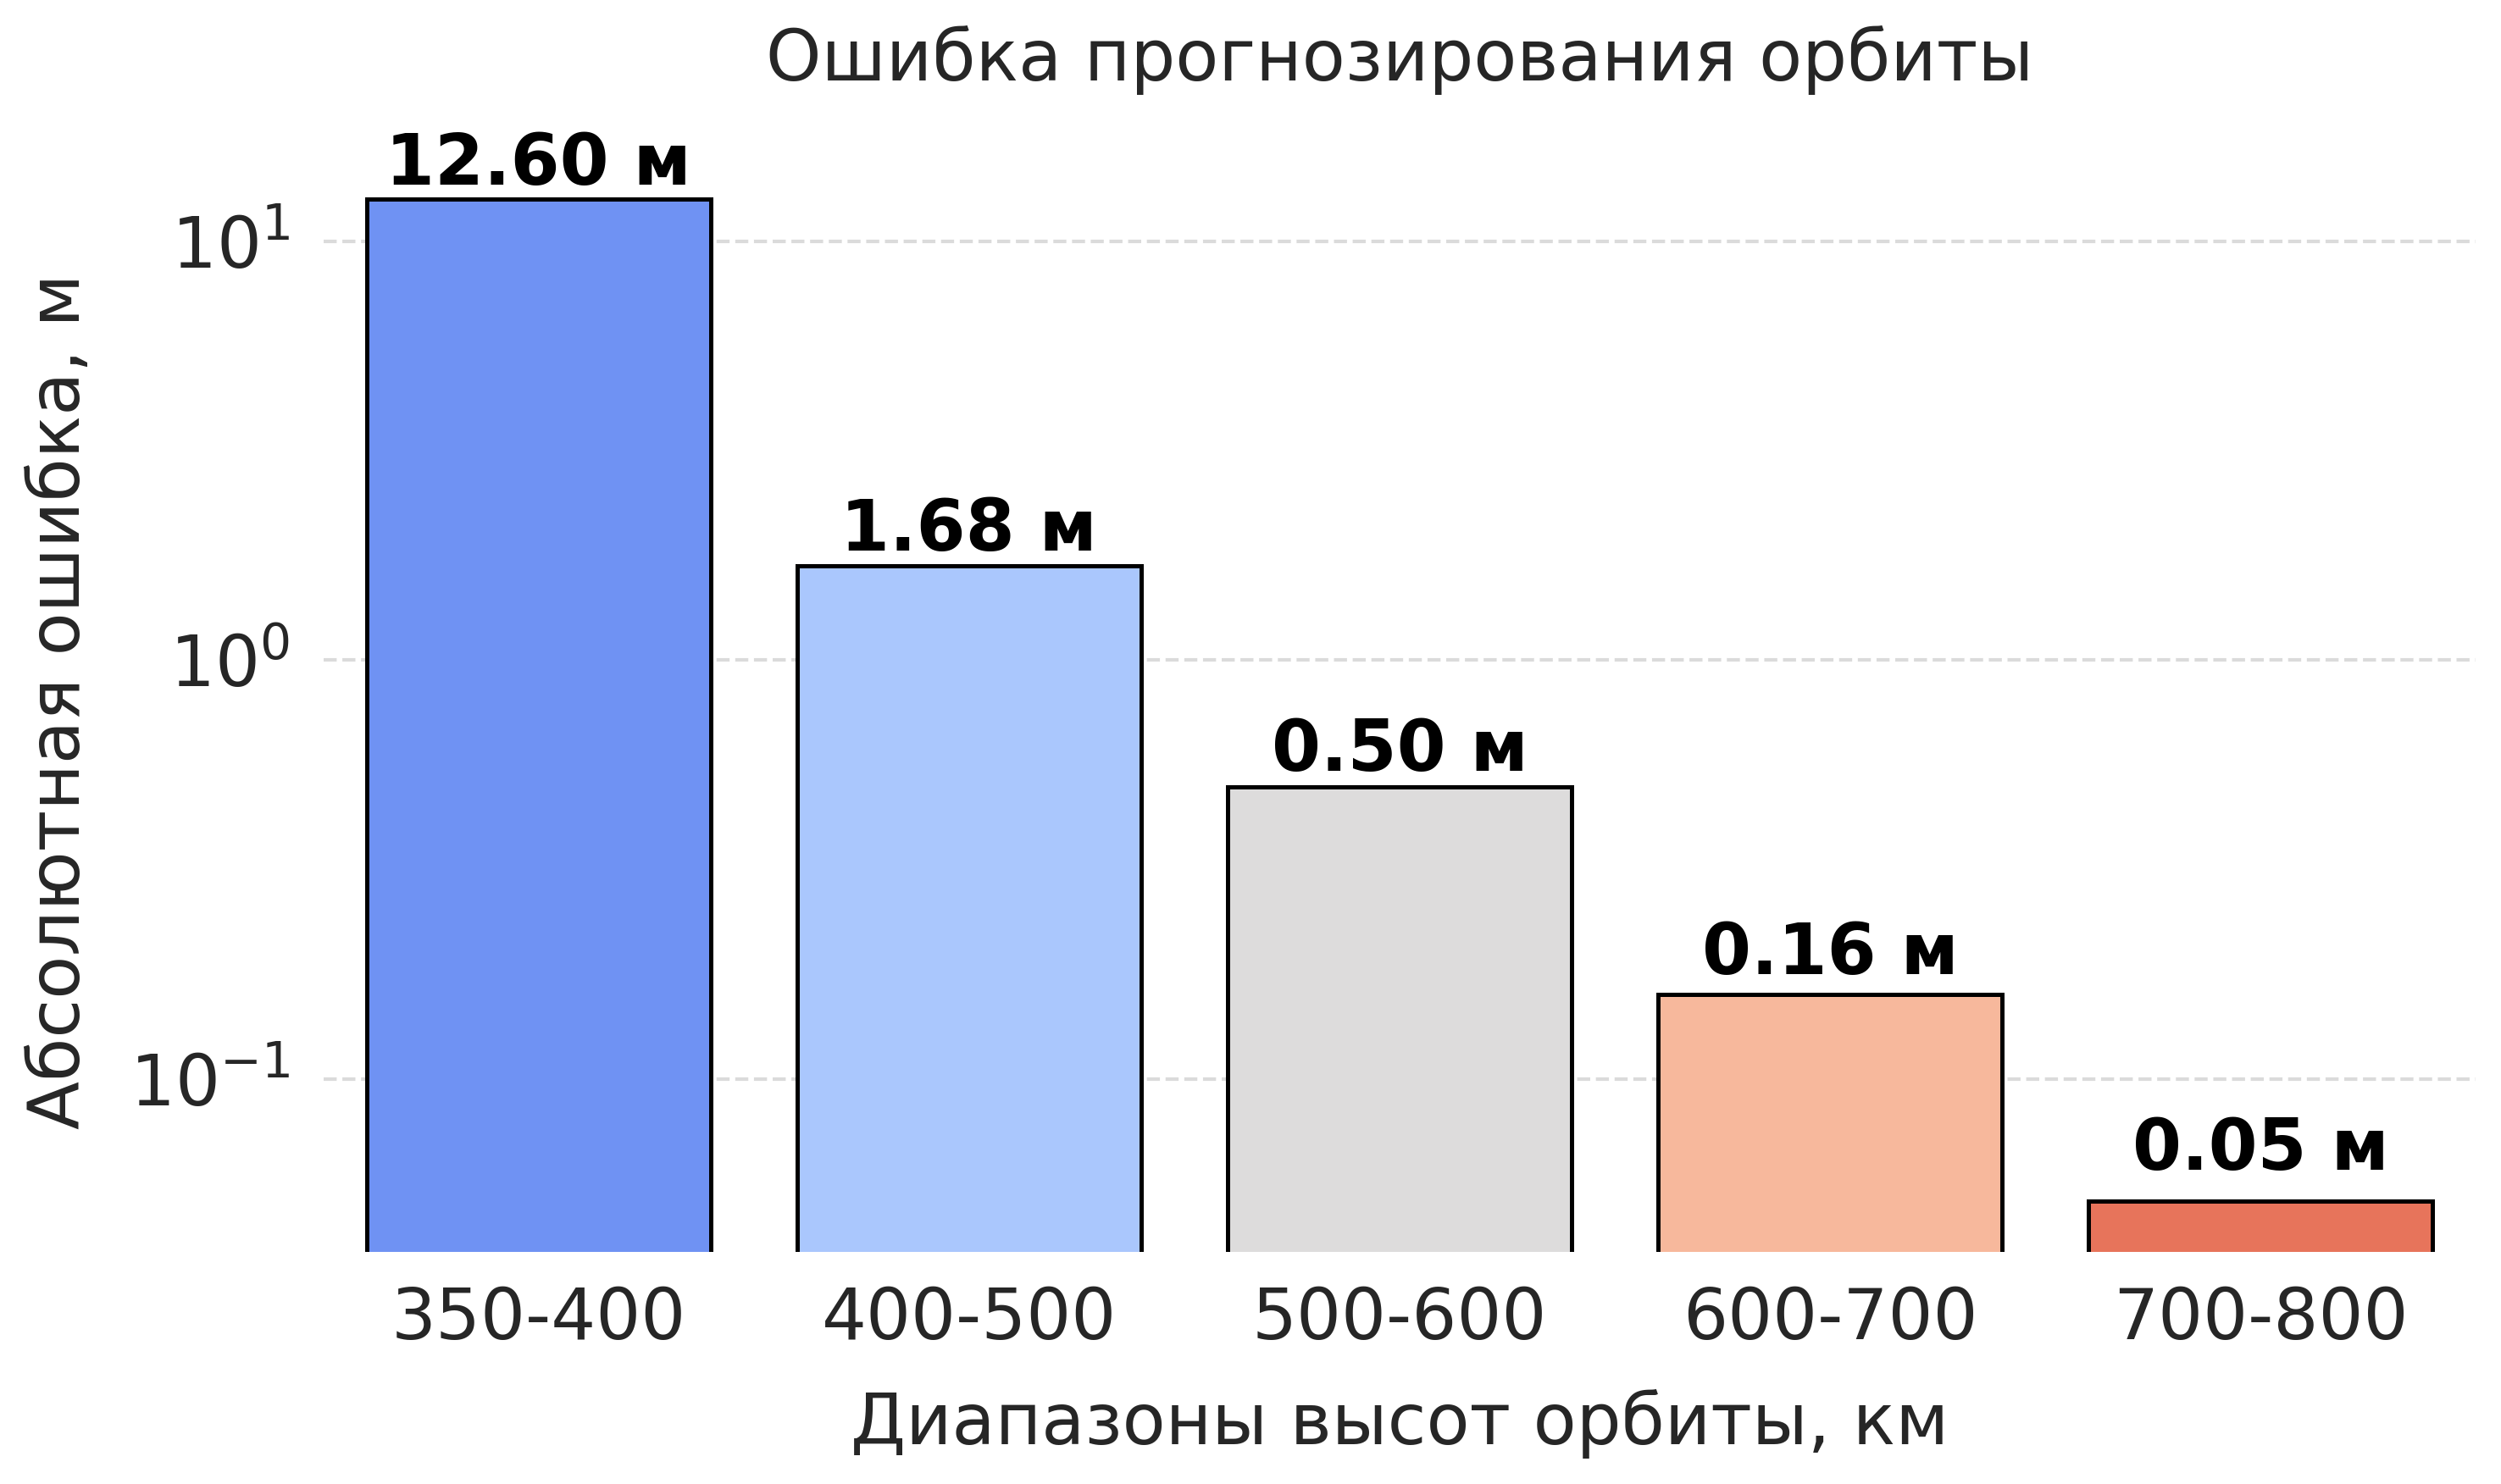
\includegraphics[width=\linewidth]{../images/solution/atmo/propagation/2573.png}
        \caption{Конфигурация (2, 5, 7, 3),
        количество ячеек (65, 25, 20, 50)}
        \label{fig:atmo:2573_propag}
    \end{subfigure}
    \hfill
    \begin{subfigure}[b]{0.48\textwidth}
        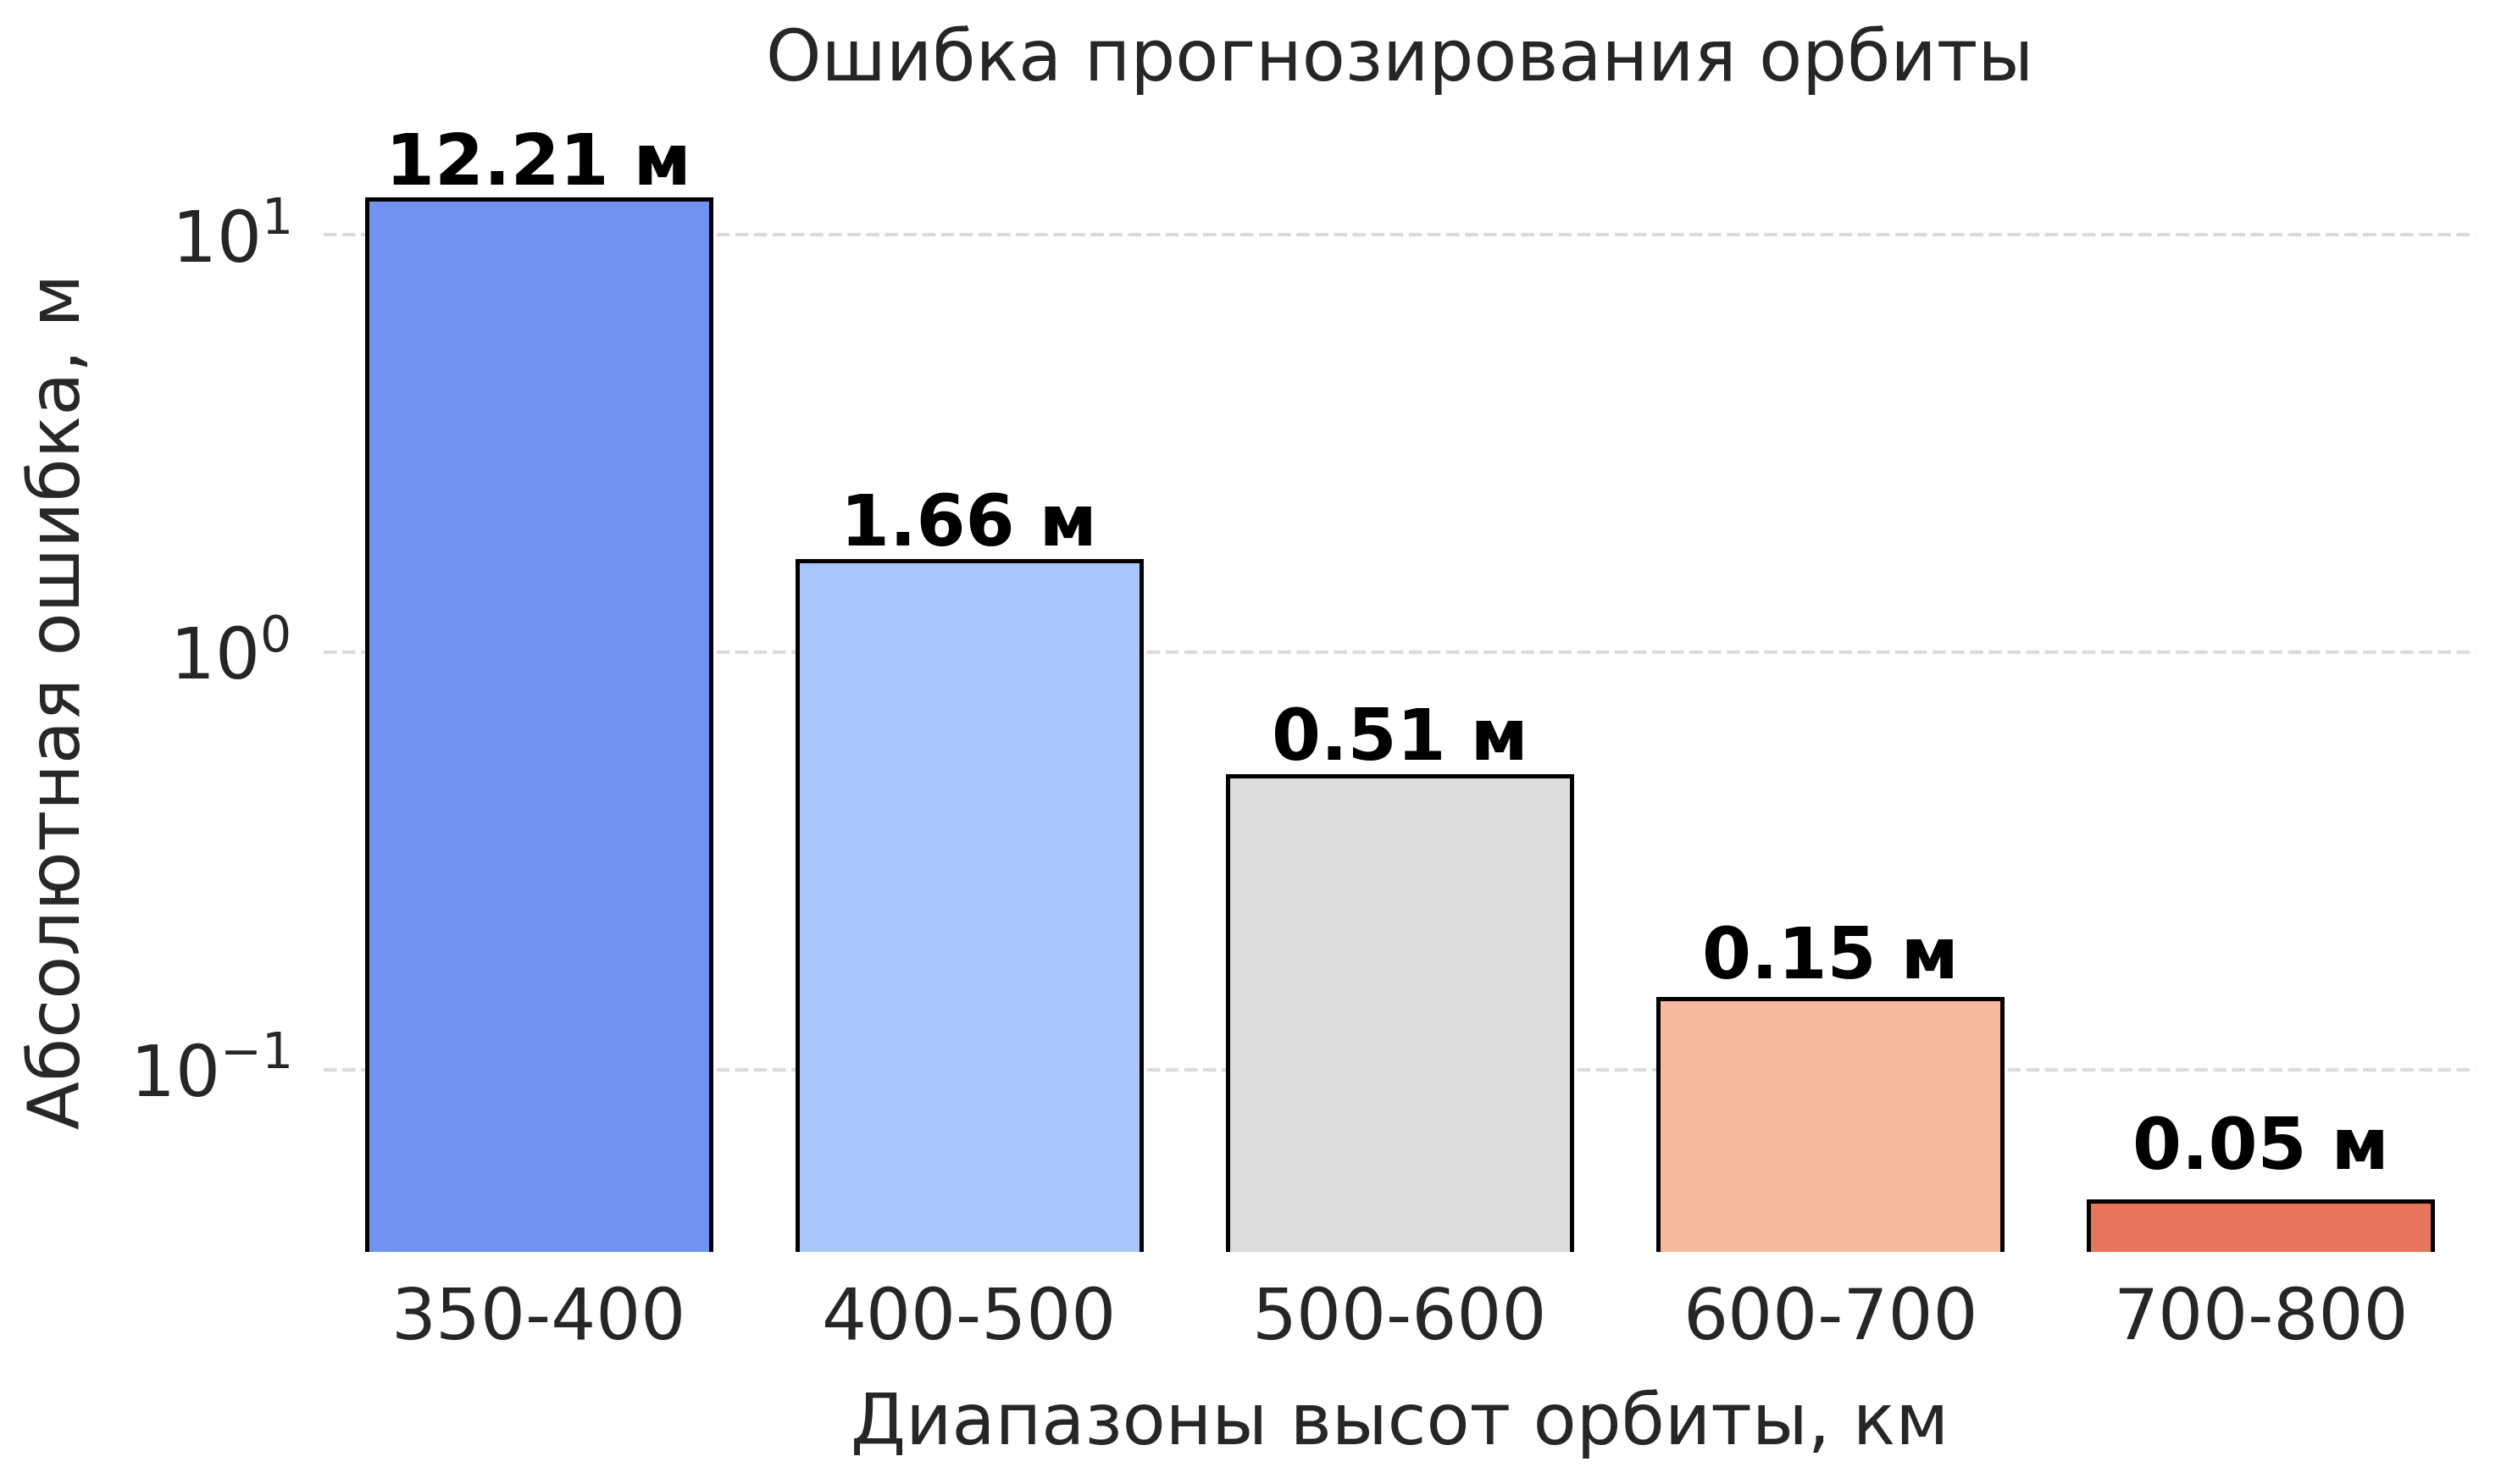
\includegraphics[width=\linewidth]{../images/solution/atmo/propagation/2735.png}
        \caption{Конфигурация (2, 7, 3, 5),
        количество ячеек (65, 15, 45, 40)}
        \label{fig:atmo:2735_propag}
    \end{subfigure}
    \caption{Зависимость ошибки прогнозирования от высоты}
    \label{fig:all_images}
\end{figure}

На заключительной стадии оценивалась возможность совместного применения интерполянтов
плотности и атмосферы. Рассмотрены орбиты с предыдущего этапа тестирования. 
Интерполянт гравитации строился по конфигурации (13, 14, 15) с числом ячеек (10, 35, 70)
на основе модели EGM2008 с 64 гармониками.
Прогноз был выполнен на 1 день. 

Сводные результаты приведены в таблице \ref{tab:atmo_propag_acc}. Из результатов следует, что интерполировать атмосферу
при прямом вычислении силы гравитационного притяжения нецелесообразно, так как ускорение
получается незначительным, в то время как появляется существенная ошибка. Интерполяция
как гравитации, так и атмосферы позволяет рассчитывать траекторию с шестикратным ускорением и
ошибкой не более 12 метров (для низких орбит).

Дальнейший анализ интерполяции атмосферы может быть связан с совершенствованием методики
поиска рациональных конфигураций и разбиений. В частности, рекомендуется
построить интерполянты с б\`{о}льшим количеством ячеек по разным координатам. Для ускорения
перебора следует использовать эмпирические зависимости, полученные из представленных в работе
результатов.

\begin{table}[h!]
    \centering
    \renewcommand{\arraystretch}{1.5}
    \begin{tabular}{|cc|cc|}
    \hline
    \multicolumn{2}{|c|}{\multirow{2}{*}{Относительная скорость прогноза}} & \multicolumn{2}{c|}{Гравитация}                         \\ \cline{3-4} 
    \multicolumn{2}{|c|}{}                                                 & \multicolumn{1}{c|}{Без интерполяции} & С интерполяцией \\ \hline
    \multicolumn{1}{|c|}{\multirow{2}{*}{Атмосфера}}   & Без интерполяции  & \multicolumn{1}{c|}{1}                & 2.8             \\ \cline{2-4} 
    \multicolumn{1}{|c|}{}                             & С интерполяцией   & \multicolumn{1}{c|}{1.2}              & 5.7             \\ \hline
    \end{tabular}
    \caption{Сводная таблица скорости прогноза}
    \label{tab:atmo_propag_acc}
\end{table}
\clearpage

\section{Параметризация модели движения}
\label{sec:Chapter2} \index{Chapter2}

Параметризованная модель движения представима в следующем виде:

\begin{equation*}
    \ddot{\mathbf{x}} = \mathbf{f}(\mathbf{x}, t) +
    \mathbf{f}_1(a_1, \dots, a_n, t),
\end{equation*}
где к исходной системе уравнений орбитальной динамики добавлена
некоторая функция, зависящая от $n$ параметров.

Неизвестные величины $a_1, \dots, a_n$ должны определяться в ходе процедуры минимизации при
восстановлении орбиты.

В настоящей работе исследуется две параметризации -- псевдоускорения и псевдоимпульсы.

\subsection{Псевдоускорения}

Псевдоускорение -- это дополнительная сила, которая действует на КО на некоторой части 
траектории. Как правило, мерный интервал разбивается на несколько участков, и на каждом
из них дополнительная сила постоянна. В некоторых случаях ускорения выбирают не
кусочно-постоянными, а кусочно-линейными для непрерывности производной силы.
Направление ускорений может быть разложено по компонентам орбитальной системы координат на радиальную, тангенциальную и нормальную
составляющие. 

Концептуальная схема применения псевдоускорений изображена на рис. \ref{fig:pseudoacc}.

\begin{figure}[h!]
    \centering
    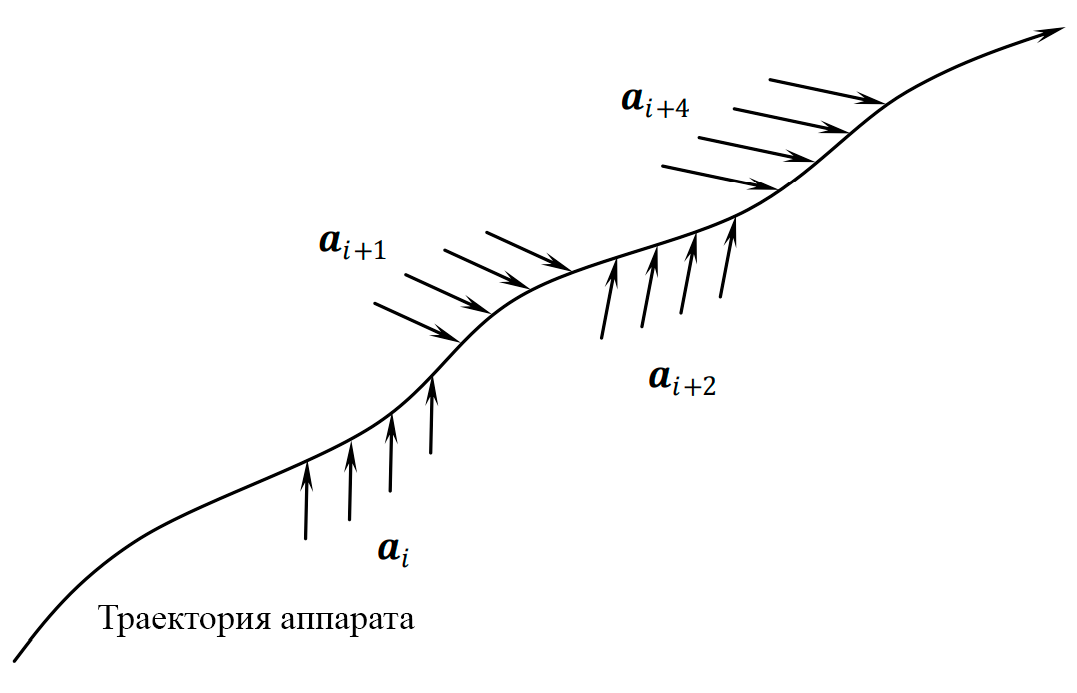
\includegraphics[width=0.8\linewidth]{../images/solution/lageos/pseudoacc.png}
    \captionof{figure}{Схема применения псевдоускорений}
    \label{fig:pseudoacc}
 \end{figure}

Уравнение движение с учетом псевдоимпульсов:
\begin{equation*}
    \ddot{\mathbf{x}} = \mathbf{f}(\mathbf{x}, t) +
        \sum_{i=0}^{n-1} \sum_{j=1}^{3} a_{i,j} \cdot \xi_{i}(t) \cdot \mathbf{e_j} (t),
\end{equation*}
где $a_{i,j}$ -- величина импульса вдоль направления $\mathbf{e_j}$.

\begin{equation*}
    \xi_{i}(t) = 
            \begin{cases}
                0, & t < t_i, \\
                1, & t_i < t < t_{i+1}, \\
                0, & t_{i+1}. \le t
            \end{cases}
\end{equation*}

Столбец матрицы изохронных производных, соответствующий параметру псевдоимпульса,
может быть вычислен в процессе интегрирования уравнения в вариациях аналогично
столбцу производных по площади аэродинамического сопротивления или солнечного давления.

\subsection{Псевдоимпульсы}

Псевдоимпульсы -- мгновенные изменения скорости в определенные моменты времени.
Эти изменения выражаются в разрыве I рода скорости, что приводит к появлению
$\delta$-функции в ускорении. При этом траектория остается непрерывной.

Схематичный вид псевдоимпульсов приведен на рис. \ref{fig:pseudoimp}

\begin{figure}[h!]
    \centering
    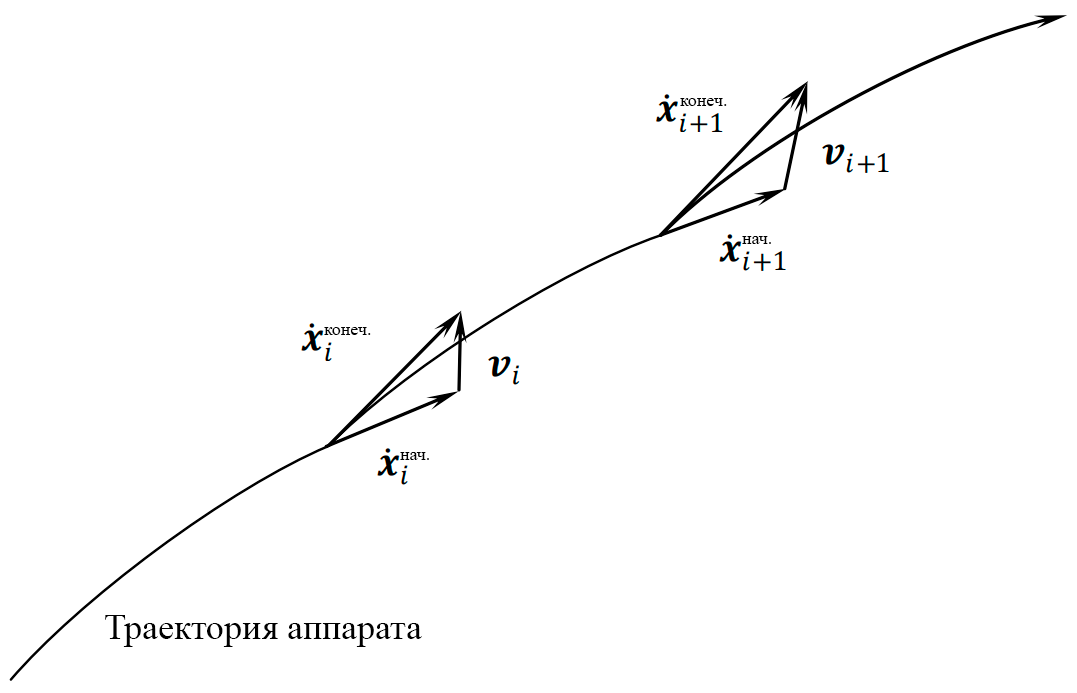
\includegraphics[width=0.8\linewidth]{../images/solution/lageos/pseudoimp.png}
    \captionof{figure}{Схема применения псевдоимпульсов}
    \label{fig:pseudoimp}
 \end{figure}

Динамика движения при наличии псевдоимпульсов описывается выражением:
\begin{equation*}
    \ddot{\mathbf{x}} = \mathbf{f}(\mathbf{x}, t) +
        \sum_{i=0}^{n-1} \sum_{j=1}^{3} v_{i,j} 
                    \cdot \delta (t - t_i) \cdot \mathbf{e_j} (t_i),
\end{equation*}
где $v_{i,j}$ -- величина импульса вдоль направления $\mathbf{e_j}$.

Получим выражение для столбца в матрице изохронных производных, соответствующего одному импульсу.
Введем функцию $U(t)$ как блок размерами 6 на 6 матрицы изохронных производных $\Phi$, отвечающий за
матрицу Якоби мгновенных элементов орбиты $\mathbf{\textbf{Э}}(t)$ по начальным элементам 
$\mathbf{\textbf{Э}}_0$:

\begin{equation*}
    U(t) = \frac{\partial \mathbf{\textbf{Э}}(t)}{\partial \mathbf{\textbf{Э}}_0}.
\end{equation*}

Пусть в момент времени $t_0$ был совершен псевдоимпульс.
Представим матрицу Якоби мгновенных элементов орбиты по элементам в момент импульса через $U(t)$:
\begin{equation*}
    \frac{\partial \mathbf{\textbf{Э}}(t)}{\partial \mathbf{\textbf{Э}}(t_0)} = 
    \frac{\partial \mathbf{\textbf{Э}}(t)}{\partial \mathbf{\textbf{Э}}_0} \cdot
    \frac{\partial \mathbf{\textbf{Э}}_0}{\partial \mathbf{\textbf{Э}}(t_0)} = 
    U(t) \cdot U(t_0)^{-1}.
\end{equation*}

Используя полученные уравнения, можно получить искомый столбец при $t > t_0$:
\begin{equation*}
    \frac{\partial \mathbf{\textbf{Э}}(t)}{\partial \mathbf{\textbf{Э}}(t_0)} = 
    \frac{\partial \mathbf{\textbf{Э}}(t)}{\partial \mathbf{\textbf{Э}}(t_0)} \cdot
    \frac{\partial \mathbf{\textbf{Э}(t_0)}}{\partial \mathbf{v}_{t_0}} =
    U(t) \cdot U(t_0)^{-1} \cdot
    \frac{\partial \mathbf{\textbf{Э}(t_0)}}{\partial \mathbf{v}_{t_0}}.
\end{equation*}

При $t < t_0$ данный столбец равен соответствующему столбцу единичной матрицы, 
так как импульс еще не был соверешен.

Заметим, что рассмотренные столбцы могут быть вычислены с минимальными дополнительными
ресурсами, так как используется уже имеющееся после прогноза решение уравения в вариациях.

\subsection{Валидация}

Тестирование программного комплекса проводилась на КА LAGEOS-2.
Измерения орбиты данного аппарата выполняются с помощью лазерной дальнометрии.
Высокоточные эфемериды LAGEOS-2 публикуются рядом агентств, 
в том числе итальянским и немецким исследовательскими центрами. Эти орбиты
были выбраны в качестве референсных. 

Сравнение эфемерид агентств показано на рис. \ref{fig:compare_agencies}. Средняя
норма разницы по положению составляет 3 сантиметра, а стандартное отклонение -- 2 сантиметра. 
Пики на графике -- псевдоимпульсы, применяемые итальянским агентством. В дальнейшем cравнение
будет проводиться именно с ним.

\begin{figure}[h!]
    \centering
    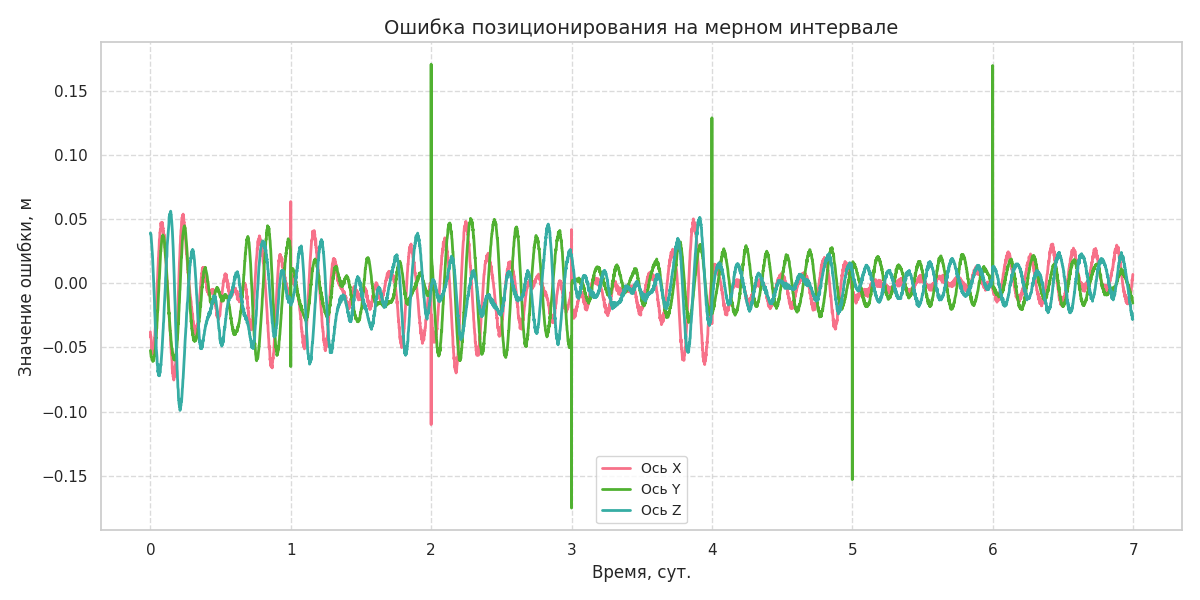
\includegraphics[width=\linewidth]{../images/solution/lageos/compare_agencies.png}
    \captionof{figure}{Разница между итальнским и немцким агентствами на мерном интервале}
    \label{fig:compare_agencies}
 \end{figure}

Характеристики аппарата и общие сведения об орбите отражены в таблицах \ref{tab:lageos2}
и \ref{tab:lageos2_orb}.

\begin{table}[h!]
    \centering
    \begin{minipage}[t]{0.48\textwidth}
    \caption{Параметры аппарата LAGEOS-2}
    \centering
    \renewcommand{\arraystretch}{1.5}
    \begin{tabular}{|l|l|}
    \hline
    \multicolumn{2}{|c|}{Параметры аппарата} \\ \hline
    Форма       & Сфера      \\ \hline
    Диаметр     & 60 см      \\ \hline
    Вес         & 405.38 кг  \\ \hline
    \end{tabular}
    \label{tab:lageos2}
    \end{minipage}
    \hfill
    \begin{minipage}[t]{0.48\textwidth}
    \caption{Параметры орбиты LAGEOS-2}
    \centering
    \renewcommand{\arraystretch}{1.5}
    \begin{tabular}{|l|l|}
    \hline
    \multicolumn{2}{|c|}{Параметры орбиты} \\ \hline
    Перигей        & 5620 км   \\ \hline
    Наклонение     & 52.64°    \\ \hline
    Эксцентриситет & 0.0135    \\ \hline
    Период         & 223 мин.  \\ \hline
    \end{tabular}
    \label{tab:lageos2_orb}
    \end{minipage}
\end{table}

Для тестирования была реализована модель движения близкая к модели агентства.
Ключевые характеристики модели представлены в таблице \ref{tab:lageos2_forces}.
Помимо геопотенциала с приливными поправками учитывалось притяжение третьих тел,
солнечное давление, эффект альбедо и релятивистские поправки. Также были применены
рассмотренные выше псевдоускорения и псевдоимпульсы. 

\begin{table}[h!]
    \caption{Параметры модели движения LAGEOS-2}
    \centering
    \renewcommand{\arraystretch}{1.5}
    \begin{tabular}{|ll|}
    \cline{1-2}
    \multicolumn{2}{|c|}{Параметры модели движения}                                                                                                                                                 \\ \hline
    \multicolumn{1}{|l|}{Геопотенциал}           & \begin{tabular}[l]{@{}l@{}}GGM02C, 70 гармоник.\\ Твердотельные и океанические \\поправки по IERS\end{tabular}                      \\ \hline
    \multicolumn{1}{|l|}{Притяжение третьих тел} & \begin{tabular}[l]{@{}l@{}}Планеты: Солнце, Меркурий, Венера, Луна, \\ Марс, Юпитер, Сатурн, Уран, Нептун.\\ Эфемериды:  JPL DE403\end{tabular} \\ \hline
    \multicolumn{1}{|l|}{Солнечное давление}     & Модель тени с перекрытием                                                                                                               \\ \hline
    \multicolumn{1}{|l|}{Эффект альбедо}         & Модель Кноке                                                                                                                            \\ \hline
    \multicolumn{1}{|l|}{Эмпирика}               & \begin{tabular}[l]{@{}l@{}}7 псевдоускорений,\\ 7 псевдоимпульсов.\\ Равномерно распределены \\ на мерном интервале\end{tabular}        \\ \hline
    \multicolumn{1}{|l|}{Релятивистские эффекты}         & по IERS                                                                                                                         \\ \hline
    \end{tabular}
    \label{tab:lageos2_forces}
\end{table}

Прогноз траектории выполнялся
методом Эверхарта 15 порядка, длина шага составила 400 секунд. 
Уточненине орбиты проводилось на мерном интервале длиной 7 суток методом Гаусса-Ньютона. 
Параметры уточнения орбиты отражены в таблице \ref{tab:lageos2_opt}.

\begin{table}[h!]
    \caption{Параметры уточнения орбиты}
    \centering
    \renewcommand{\arraystretch}{1.5}
    \begin{tabular}{|ll|}
    \hline
    \multicolumn{2}{|c|}{Параметры уточнения орбиты}                                                                                \\ \hline
    \multicolumn{1}{|l|}{Интегрирование}  & \begin{tabular}[c]{@{}l@{}}Метод Эверхарта 15 порядка\\ с шагом 400 секунд\end{tabular} \\ \hline
    \multicolumn{1}{|l|}{Оптимизация}     & Метод Гаусса-Ньютона                                                                    \\ \hline
    \multicolumn{1}{|l|}{Тип измерений}   & Положение, скорость                                                                     \\ \hline
    \multicolumn{1}{|l|}{Целевая функция} & Сумма квадратов невязок                                                                 \\ \hline
    \multicolumn{1}{|l|}{Мерный интервал} & 7 суток (30.05.2021 -- 06.06.2021)                                                                                 \\ \hline
    \end{tabular}
    \label{tab:lageos2_opt}
\end{table}

Проведена серия численных экспериментов, в которых модель сил поэтапно дополнялась.
Это позволило увидеть динамику снижения ошибки на мерном интервале при учете различных
факторов. Результаты экспериментов представлены в таблице \ref{tab:lageos2_exp} и
на рис. \ref{fig:step_by_step}. 

\begin{table}[h!]
    \caption{Зависимость точности восстановления орбиты от учета различных наборов
    возмущающих факторов}
    \centering
    \renewcommand{\arraystretch}{1.5}
    \begin{tabular}{|l|lll|}
    \hline
    \multicolumn{1}{|c|}{\multirow{2}{*}{Набор сил}} & \multicolumn{3}{c|}{Ошибка на мерном интервале, м}                                                             \\ \cline{2-4} 
    \multicolumn{1}{|c|}{}                           & \multicolumn{1}{c|}{Максимальная} & \multicolumn{1}{c|}{Средняя} & \multicolumn{1}{c|}{Стандартное отклонение} \\ \hline
    Потенциал с J2                                   & \multicolumn{1}{l|}{432}          & \multicolumn{1}{l|}{161}     & 183                                         \\ \hline
    70 гармоник                                      & \multicolumn{1}{l|}{327}          & \multicolumn{1}{l|}{96}      & 115                                         \\ \hline
    + притяжение третьих тел                         & \multicolumn{1}{l|}{7.4}          & \multicolumn{1}{l|}{2.3}     & 2.7                                         \\ \hline
    + солнечное давление                             & \multicolumn{1}{l|}{2.8}          & \multicolumn{1}{l|}{0.9}     & 1.0                                         \\ \hline
    + приливные поправки                             & \multicolumn{1}{l|}{0.76}         & \multicolumn{1}{l|}{0.26}    & 0.29                                        \\ \hline
    + эффект альбедо                                 & \multicolumn{1}{l|}{0.48}         & \multicolumn{1}{l|}{0.13}    & 0.15                                        \\ \hline
    + 7 псевдоускорений                              & \multicolumn{1}{l|}{0.29}         & \multicolumn{1}{l|}{0.10}    & 0.11                                        \\ \hline
    + 7 псевдоимпульсов                              & \multicolumn{1}{l|}{0.11}         & \multicolumn{1}{l|}{0.05}    & 0.06                                        \\ \hline
    \end{tabular}
    \label{tab:lageos2_exp}
\end{table}

\begin{figure}[h!]
    \centering
    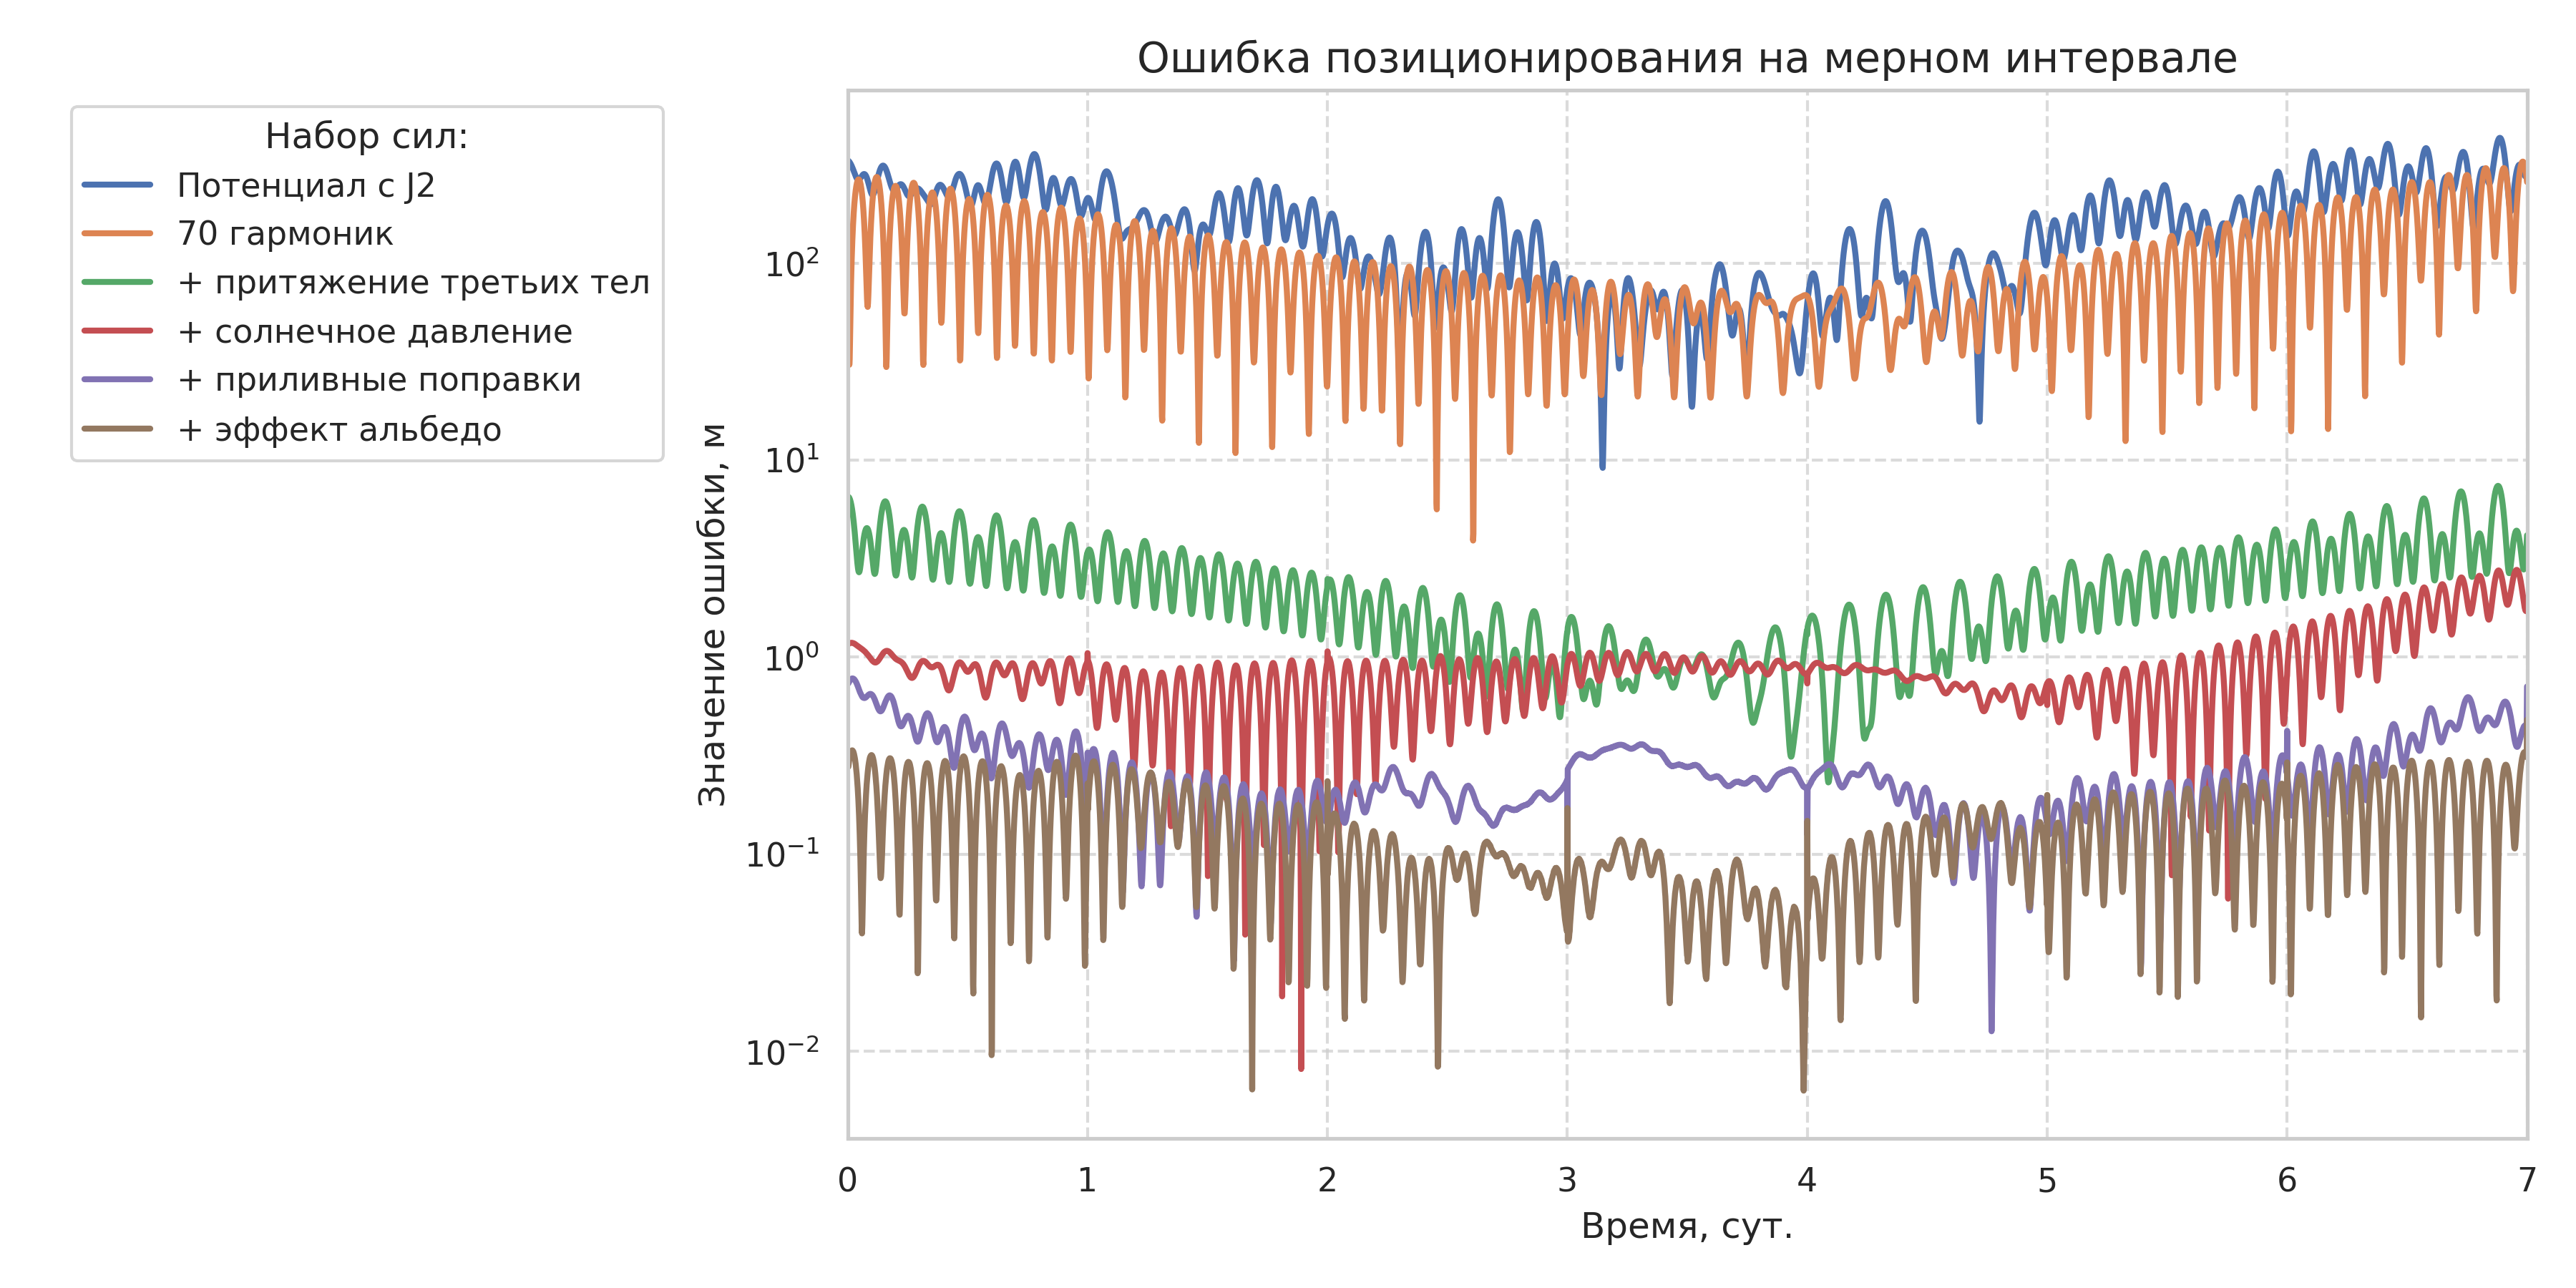
\includegraphics[width=\linewidth]{../images/solution/lageos/step_by_step.png}
    \captionof{figure}{График невязок на мерном интервале при использовании различных наборов сил
    и псевдоимпульсами}
    \label{fig:step_by_step}
 \end{figure}

Из результатов следует, что основные возмущающие факторы -- это нецентральность поля Земли,
притяжение третьих тел и солнечное давление. Учет этих сил позволяет получить среднюю
ошибку на мерном интервале меньше метра. Вклад приливных поправок и эффекта альбедо
значительно меньше. Таким образом, полная модель сил без параметризации дает среднюю ошибку
13 см.

Получить дециметровую точность помогает использвоние псевдоускорений. Данный подход
существенно уменьшает максимальную ошибку и сводит среднюю невзяку и стандартное отклонение
 к 10 и 11 сантиметрам соответственно. Для восстановления орбиты с субдециметровой точностью
 можно повышать количество псевдоускорений или добавить псевдоимпульсы. С комбинацией
 из 7 ускорений и 7 псевдоимпульсов средняя ошибка на мерном интервале падает до 5 см. 
 Такое значение ошибок близко к разнице между двумя агентствами, поэтому
 уточнение орбиты можно считать успешным.

Графики невязок на мерном интервале показаны на рис. \ref{fig:no_imp_no_acc}, 
\ref{fig:no_imp_with_acc}, \ref{fig:with_imp_with_acc}.

\begin{figure}[h!]
   \centering
   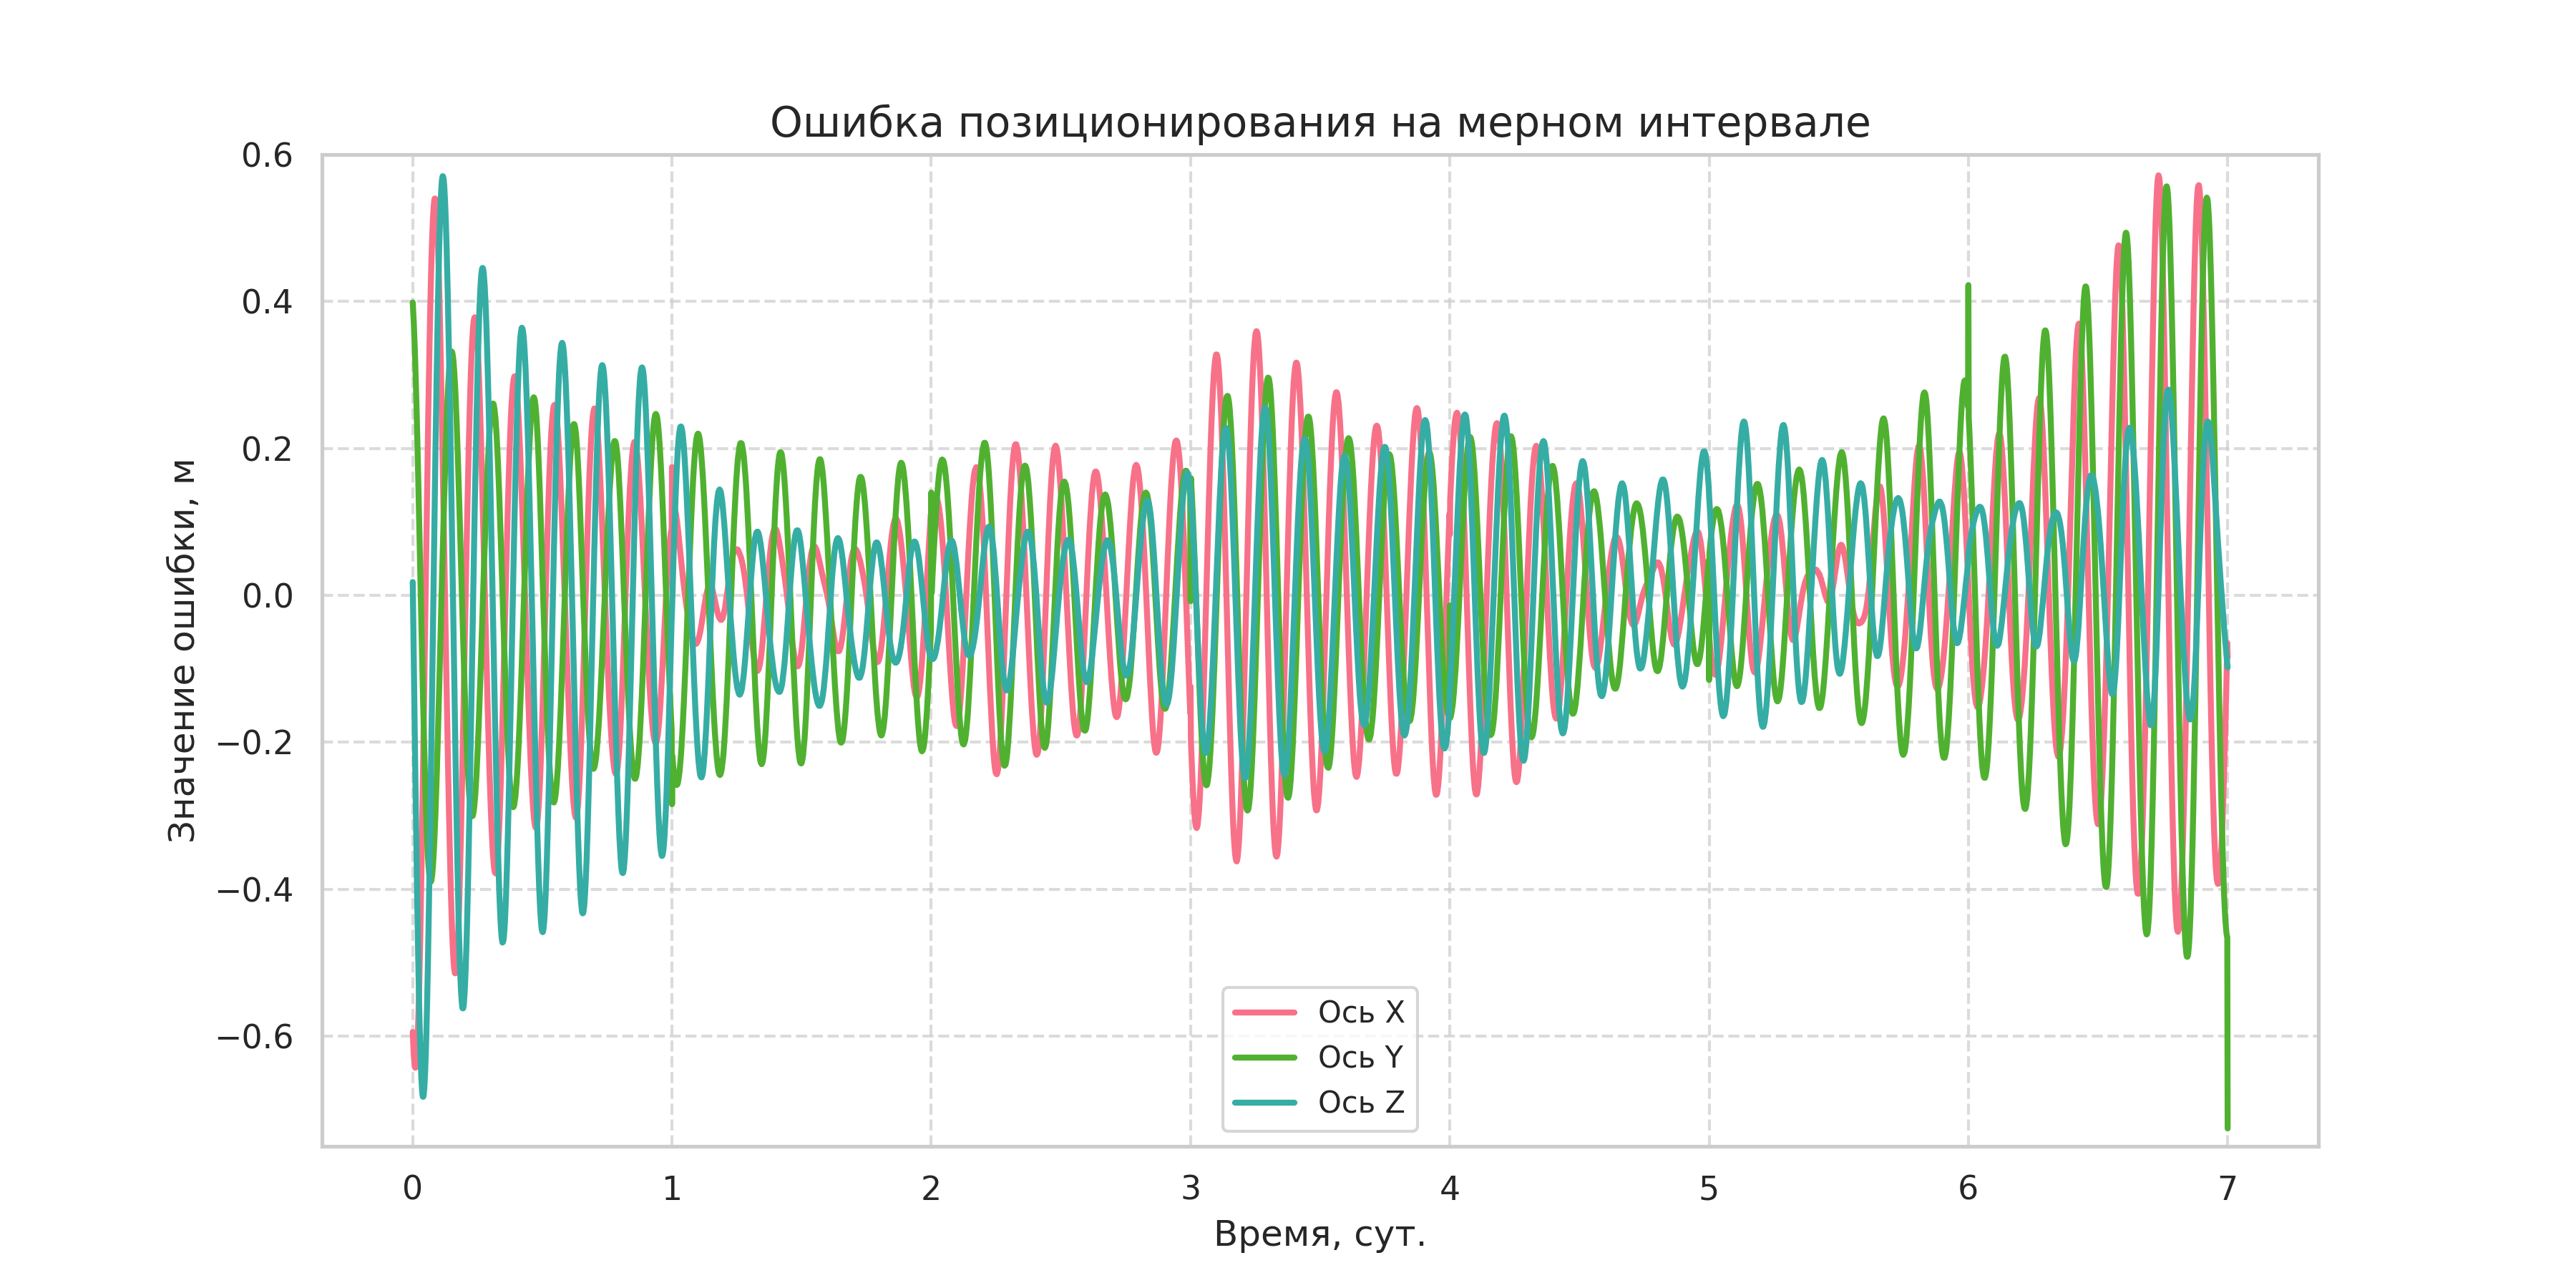
\includegraphics[width=\linewidth]{../images/solution/lageos/no_imp_no_acc.png}
   \captionof{figure}{График невязок на мерном интервале при использовании модели сил без параметризации}
   \label{fig:no_imp_no_acc}
\end{figure}

\begin{figure}[h!]
   \centering
   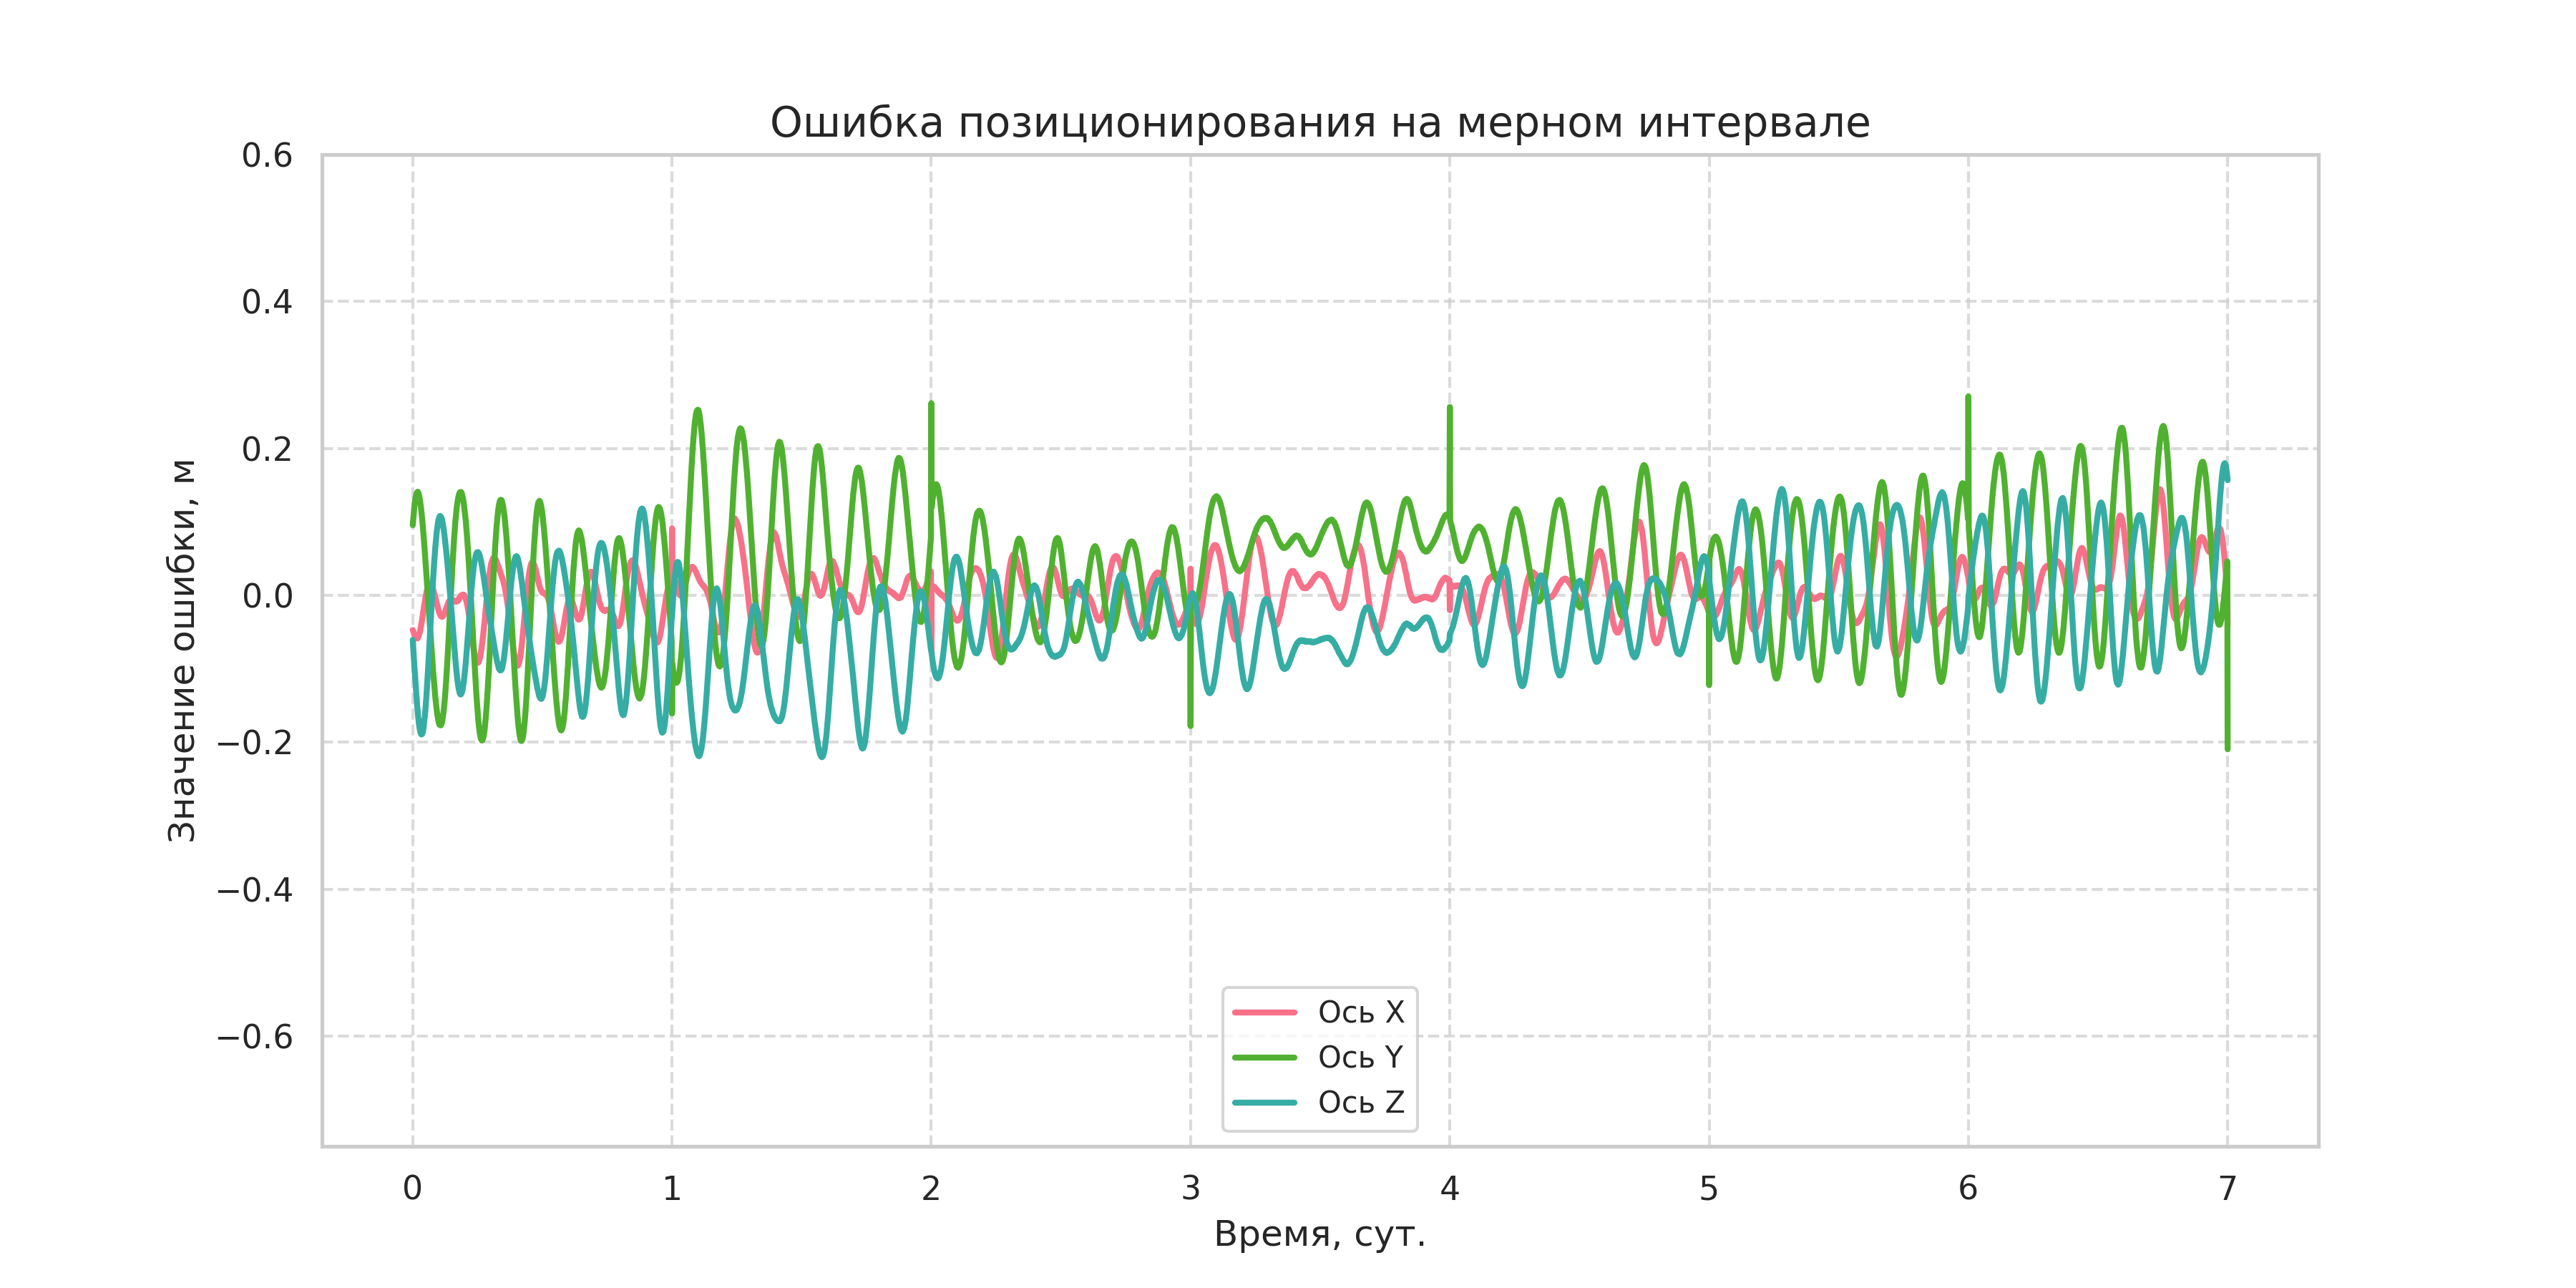
\includegraphics[width=\linewidth]{../images/solution/lageos/no_imp_with_acc.png}
   \captionof{figure}{График невязок на мерном интервале при использовании модели сил c псевдоускорениями}
   \label{fig:no_imp_with_acc}
\end{figure}

\begin{figure}[h!]
   \centering
   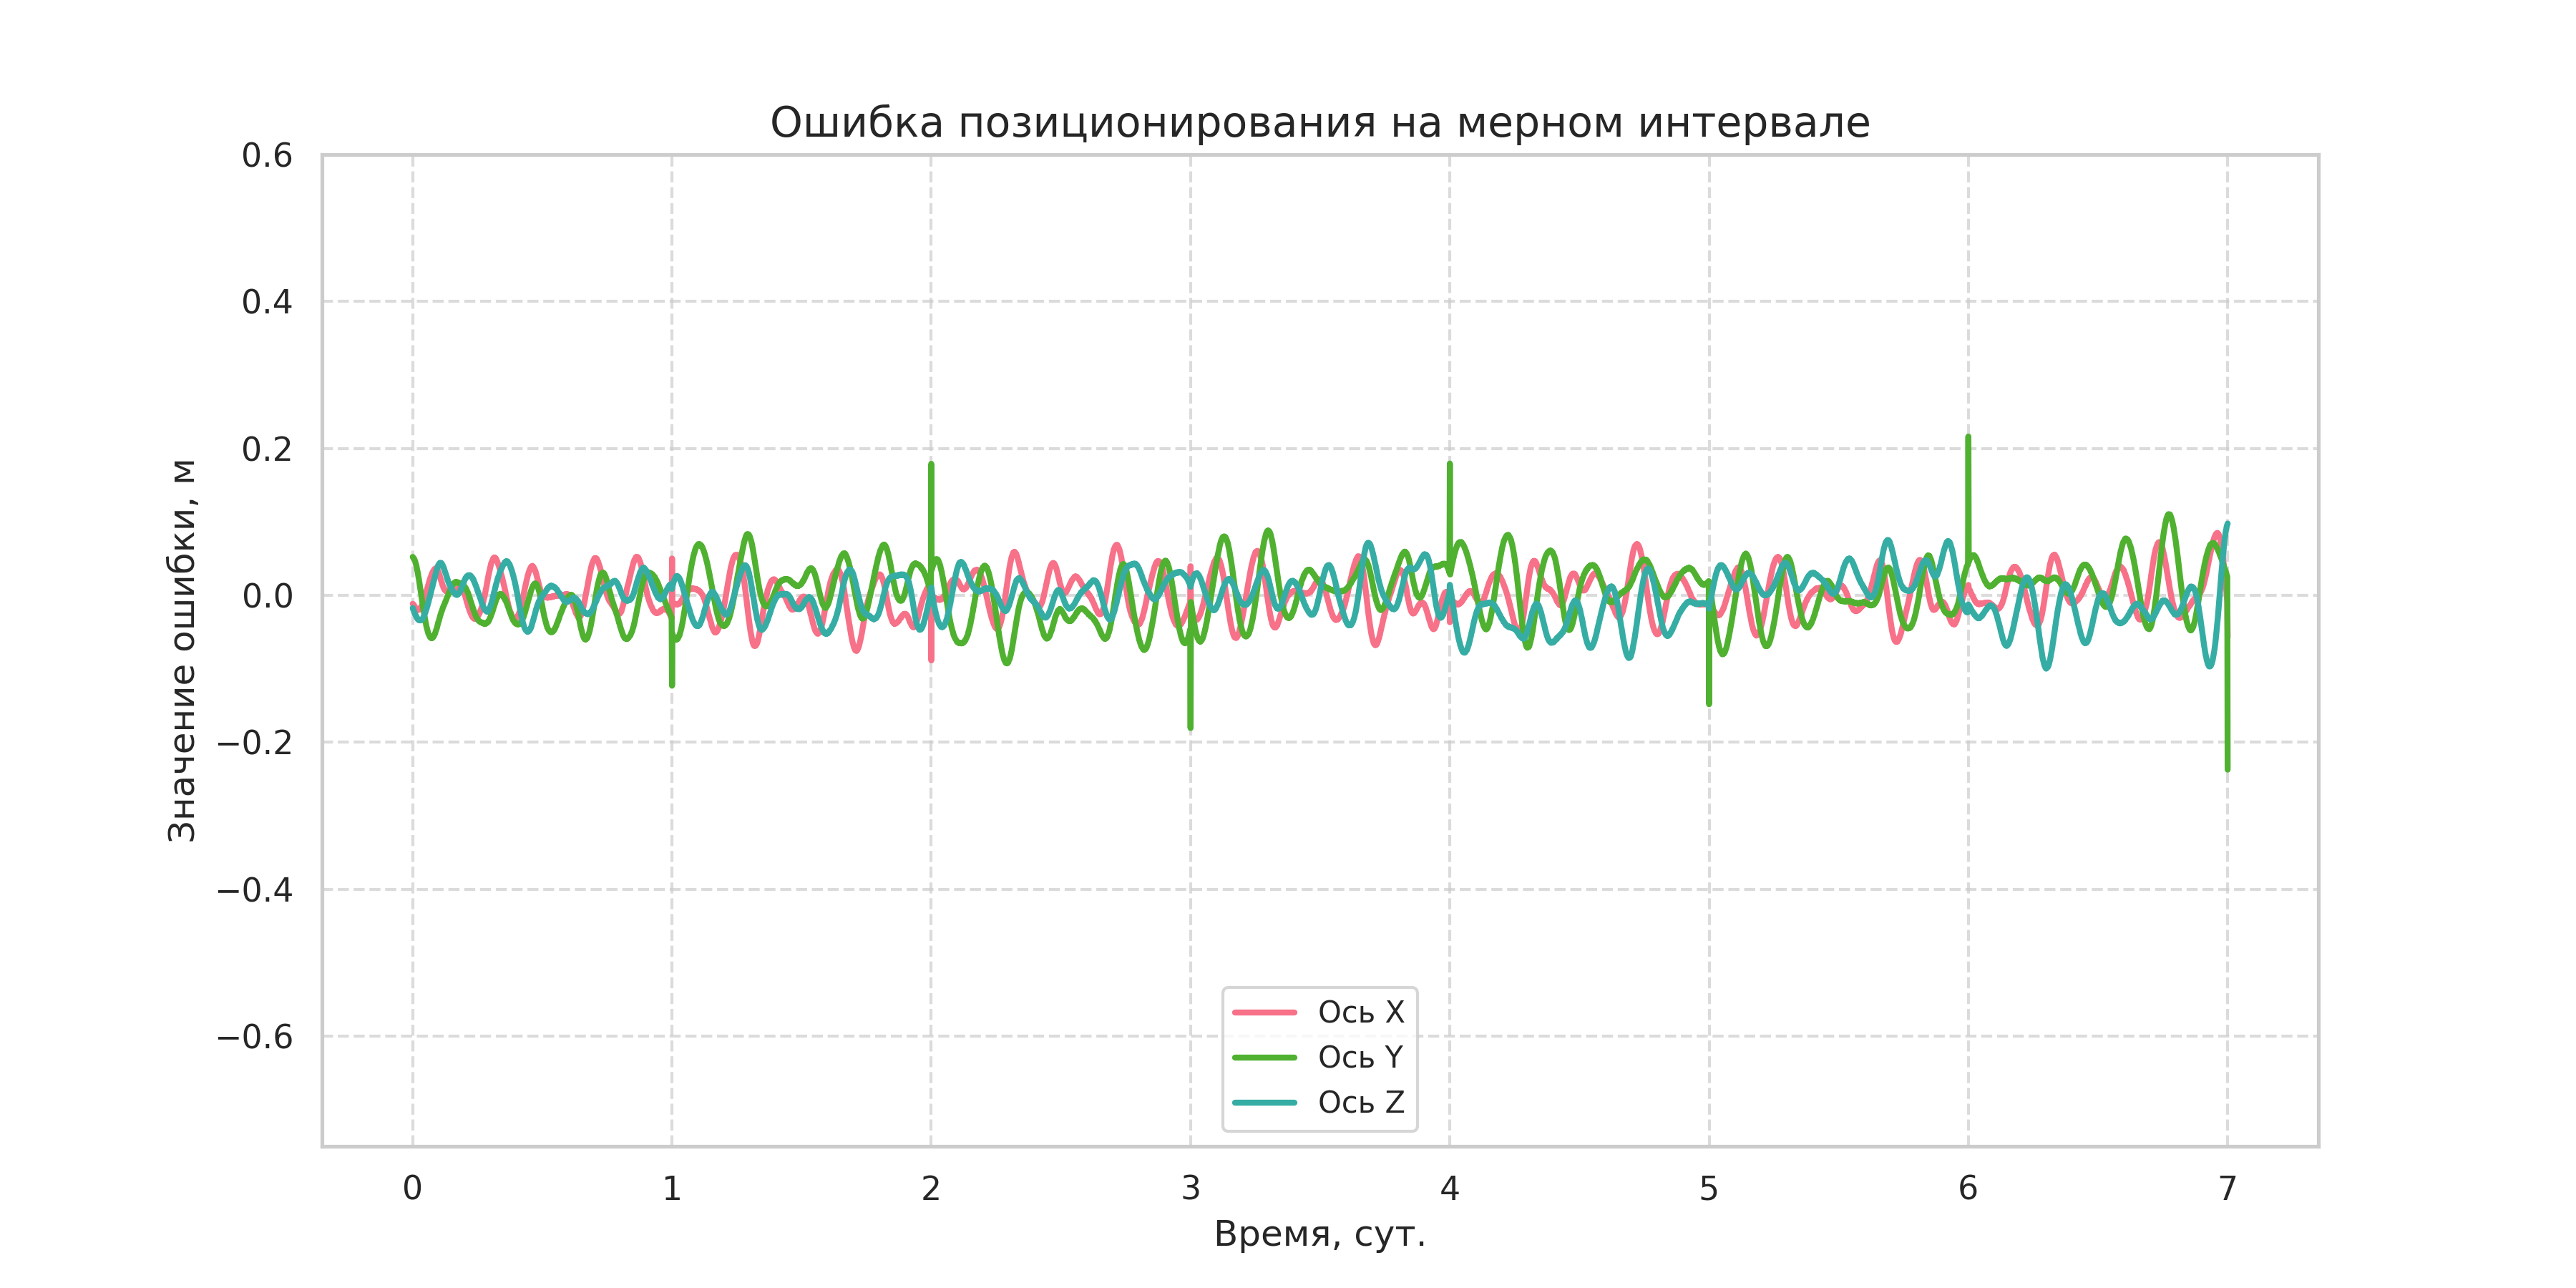
\includegraphics[width=\linewidth]{../images/solution/lageos/with_imp_with_acc.png}
   \captionof{figure}{График невязок на мерном интервале при использовании модели сил с псевдоускорениями
   и псевдоимпульсами}
   \label{fig:with_imp_with_acc}
\end{figure}

На рис. \ref{fig:no_imp_no_acc} хорошо видна специфика работы метода наименьших квадратов.
Метод оптимизрует решение таким образом, что в центральной области невязка получается
минимальной, а по краям симметрично растет. Это свидетельствует о правильной работе
алгоритма восстановления орбиты.

Валидация пройдена.

\newpage
    \section{Верификация}
\label{sec:Chapter3} \index{Chapter2}

Проведено тестирование точности различных конфигураций интерполянтов для модели NRLMSISE-00.

Диапазон интерполяции по расстоянию был выбран от 350 до 800 километров, интервал по времени
составил одни сутки. В ходе тестов была использована космическая погода за 11 января 2014 года.
Этот год соответствует высокой солнечной активности, что позволяет протестировать качество
интерполяции в сложных условиях.

Сетка для тестирования алгоритма состояла из более 1 миллиона точек, равномерно
распределенных по области интерполяции. Для каждого интерполянта измерялась максимальная
ошибка на тестовой сетке, размер и величина ускорения по сравнению с прямым расчетом плотности.

Полный перебор по возможным конфигурациям и количеству ячеек интерполянтов сложен
из-за большого количества вариантов, времени, затрачиваемого на построение каждого интерполянта и
занимаемой памяти. Поэтому поиск подходящих параметров проводился поэтапно.

Учитывая близкую к линейной зависимость логарифма плотности от высоты, для этой координаты
была выбрана наименьшая степень полинома -- 2. По времени была установлена степень 7,
чтобы добиться высокой точности при меньшем количестве точек и иметь возможность
построения интерполянта на более длительные интервалы времени без потери точности. 
В рассмотрении остались наборы (2, 3, 5, 7) и (2, 5, 3, 7). Интерполянты для полиномов более
высоких порядков не строились из-за снижения производительности таких конфигураций и
существенного повышения затрат памяти для хранения коэффициентов.

Для каждого набора было зафиксировано количество ячеек по высоте -- 65. Количество ячеек
по широте, долготе и времени варьировалось от 5 до 50. Эмпирически определялось
количество ячеек для достижения точности при заданном разбиении по высоте. Далее
для интерполянтов с параметрами, выбранными на предыдущем шаге, варьировалось
количество ячеек по высоте и определялась точность, достижимая с такими параметрами.


\newpage
    \section{Валидация}
\label{sec:Chapter4} \index{Chapter2}

\section{Параметризация модели движения}
\label{sec:Chapter2} \index{Chapter2}

Параметризованная модель движения представима в следующем виде:

\begin{equation*}
    \ddot{\mathbf{x}} = \mathbf{f}(\mathbf{x}, t) +
    \mathbf{f}_1(a_1, \dots, a_n, t),
\end{equation*}
где к исходной системе уравнений орбитальной динамики добавлена
некоторая функция, зависящая от $n$ параметров.

Неизвестные величины $a_1, \dots, a_n$ должны определяться в ходе процедуры минимизации при
восстановлении орбиты.

В настоящей работе исследуется две параметризации -- псевдоускорения и псевдоимпульсы.

\subsection{Псевдоускорения}

Псевдоускорение -- это дополнительная сила, которая действует на КО на некоторой части 
траектории. Как правило, мерный интервал разбивается на несколько участков, и на каждом
из них дополнительная сила постоянна. В некоторых случаях ускорения выбирают не
кусочно-постоянными, а кусочно-линейными для непрерывности производной силы.
Направление ускорений может быть разложено по компонентам орбитальной системы координат на радиальную, тангенциальную и нормальную
составляющие. 

Концептуальная схема применения псевдоускорений изображена на рис. \ref{fig:pseudoacc}.

\begin{figure}[h!]
    \centering
    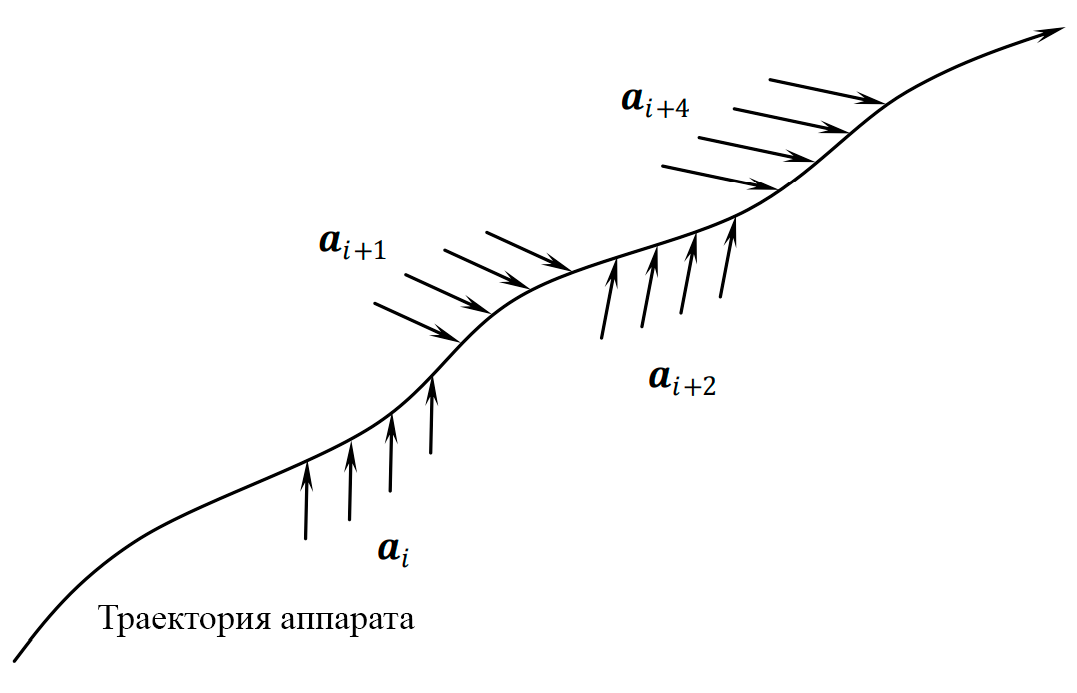
\includegraphics[width=0.8\linewidth]{../images/solution/lageos/pseudoacc.png}
    \captionof{figure}{Схема применения псевдоускорений}
    \label{fig:pseudoacc}
 \end{figure}

Уравнение движение с учетом псевдоимпульсов:
\begin{equation*}
    \ddot{\mathbf{x}} = \mathbf{f}(\mathbf{x}, t) +
        \sum_{i=0}^{n-1} \sum_{j=1}^{3} a_{i,j} \cdot \xi_{i}(t) \cdot \mathbf{e_j} (t),
\end{equation*}
где $a_{i,j}$ -- величина импульса вдоль направления $\mathbf{e_j}$.

\begin{equation*}
    \xi_{i}(t) = 
            \begin{cases}
                0, & t < t_i, \\
                1, & t_i < t < t_{i+1}, \\
                0, & t_{i+1}. \le t
            \end{cases}
\end{equation*}

Столбец матрицы изохронных производных, соответствующий параметру псевдоимпульса,
может быть вычислен в процессе интегрирования уравнения в вариациях аналогично
столбцу производных по площади аэродинамического сопротивления или солнечного давления.

\subsection{Псевдоимпульсы}

Псевдоимпульсы -- мгновенные изменения скорости в определенные моменты времени.
Эти изменения выражаются в разрыве I рода скорости, что приводит к появлению
$\delta$-функции в ускорении. При этом траектория остается непрерывной.

Схематичный вид псевдоимпульсов приведен на рис. \ref{fig:pseudoimp}

\begin{figure}[h!]
    \centering
    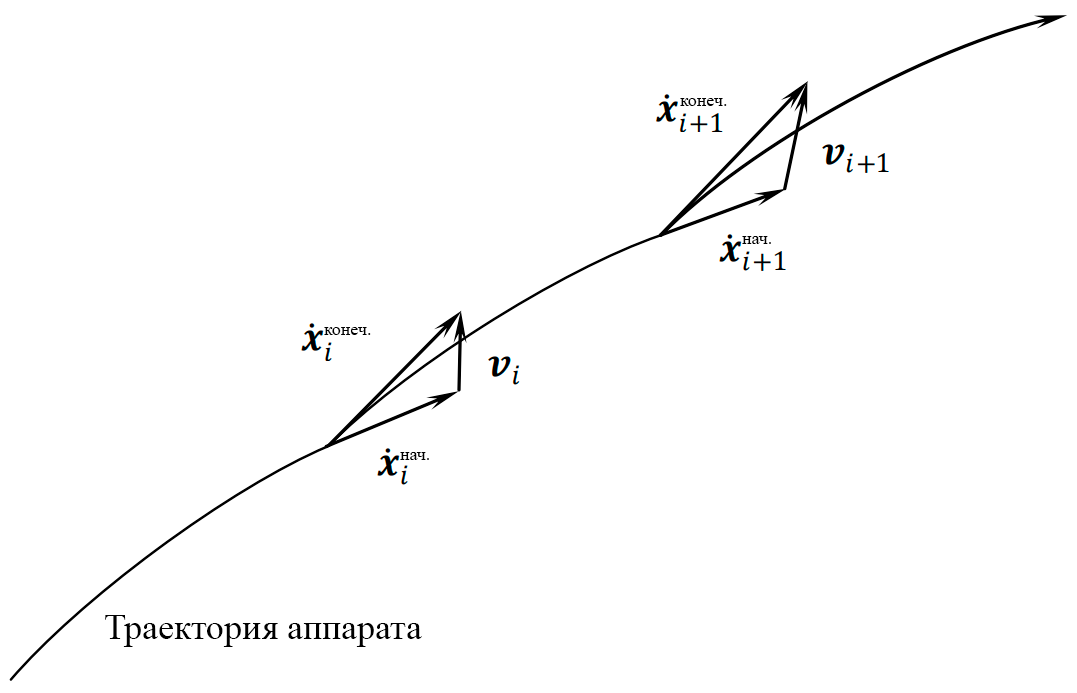
\includegraphics[width=0.8\linewidth]{../images/solution/lageos/pseudoimp.png}
    \captionof{figure}{Схема применения псевдоимпульсов}
    \label{fig:pseudoimp}
 \end{figure}

Динамика движения при наличии псевдоимпульсов описывается выражением:
\begin{equation*}
    \ddot{\mathbf{x}} = \mathbf{f}(\mathbf{x}, t) +
        \sum_{i=0}^{n-1} \sum_{j=1}^{3} v_{i,j} 
                    \cdot \delta (t - t_i) \cdot \mathbf{e_j} (t_i),
\end{equation*}
где $v_{i,j}$ -- величина импульса вдоль направления $\mathbf{e_j}$.

Получим выражение для столбца в матрице изохронных производных, соответствующего одному импульсу.
Введем функцию $U(t)$ как блок размерами 6 на 6 матрицы изохронных производных $\Phi$, отвечающий за
матрицу Якоби мгновенных элементов орбиты $\mathbf{\textbf{Э}}(t)$ по начальным элементам 
$\mathbf{\textbf{Э}}_0$:

\begin{equation*}
    U(t) = \frac{\partial \mathbf{\textbf{Э}}(t)}{\partial \mathbf{\textbf{Э}}_0}.
\end{equation*}

Пусть в момент времени $t_0$ был совершен псевдоимпульс.
Представим матрицу Якоби мгновенных элементов орбиты по элементам в момент импульса через $U(t)$:
\begin{equation*}
    \frac{\partial \mathbf{\textbf{Э}}(t)}{\partial \mathbf{\textbf{Э}}(t_0)} = 
    \frac{\partial \mathbf{\textbf{Э}}(t)}{\partial \mathbf{\textbf{Э}}_0} \cdot
    \frac{\partial \mathbf{\textbf{Э}}_0}{\partial \mathbf{\textbf{Э}}(t_0)} = 
    U(t) \cdot U(t_0)^{-1}.
\end{equation*}

Используя полученные уравнения, можно получить искомый столбец при $t > t_0$:
\begin{equation*}
    \frac{\partial \mathbf{\textbf{Э}}(t)}{\partial \mathbf{\textbf{Э}}(t_0)} = 
    \frac{\partial \mathbf{\textbf{Э}}(t)}{\partial \mathbf{\textbf{Э}}(t_0)} \cdot
    \frac{\partial \mathbf{\textbf{Э}(t_0)}}{\partial \mathbf{v}_{t_0}} =
    U(t) \cdot U(t_0)^{-1} \cdot
    \frac{\partial \mathbf{\textbf{Э}(t_0)}}{\partial \mathbf{v}_{t_0}}.
\end{equation*}

При $t < t_0$ данный столбец равен соответствующему столбцу единичной матрицы, 
так как импульс еще не был соверешен.

Заметим, что рассмотренные столбцы могут быть вычислены с минимальными дополнительными
ресурсами, так как используется уже имеющееся после прогноза решение уравения в вариациях.

\subsection{Валидация}

Тестирование программного комплекса проводилась на КА LAGEOS-2.
Измерения орбиты данного аппарата выполняются с помощью лазерной дальнометрии.
Высокоточные эфемериды LAGEOS-2 публикуются рядом агентств, 
в том числе итальянским и немецким исследовательскими центрами. Эти орбиты
были выбраны в качестве референсных. 

Сравнение эфемерид агентств показано на рис. \ref{fig:compare_agencies}. Средняя
норма разницы по положению составляет 3 сантиметра, а стандартное отклонение -- 2 сантиметра. 
Пики на графике -- псевдоимпульсы, применяемые итальянским агентством. В дальнейшем cравнение
будет проводиться именно с ним.

\begin{figure}[h!]
    \centering
    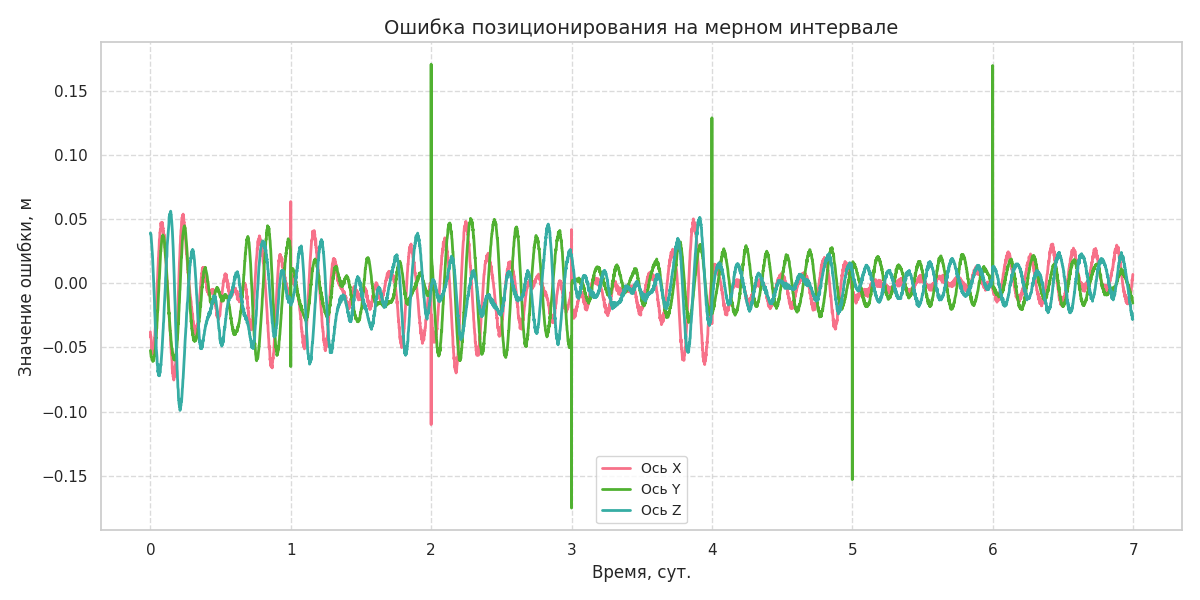
\includegraphics[width=\linewidth]{../images/solution/lageos/compare_agencies.png}
    \captionof{figure}{Разница между итальнским и немцким агентствами на мерном интервале}
    \label{fig:compare_agencies}
 \end{figure}

Характеристики аппарата и общие сведения об орбите отражены в таблицах \ref{tab:lageos2}
и \ref{tab:lageos2_orb}.

\begin{table}[h!]
    \centering
    \begin{minipage}[t]{0.48\textwidth}
    \caption{Параметры аппарата LAGEOS-2}
    \centering
    \renewcommand{\arraystretch}{1.5}
    \begin{tabular}{|l|l|}
    \hline
    \multicolumn{2}{|c|}{Параметры аппарата} \\ \hline
    Форма       & Сфера      \\ \hline
    Диаметр     & 60 см      \\ \hline
    Вес         & 405.38 кг  \\ \hline
    \end{tabular}
    \label{tab:lageos2}
    \end{minipage}
    \hfill
    \begin{minipage}[t]{0.48\textwidth}
    \caption{Параметры орбиты LAGEOS-2}
    \centering
    \renewcommand{\arraystretch}{1.5}
    \begin{tabular}{|l|l|}
    \hline
    \multicolumn{2}{|c|}{Параметры орбиты} \\ \hline
    Перигей        & 5620 км   \\ \hline
    Наклонение     & 52.64°    \\ \hline
    Эксцентриситет & 0.0135    \\ \hline
    Период         & 223 мин.  \\ \hline
    \end{tabular}
    \label{tab:lageos2_orb}
    \end{minipage}
\end{table}

Для тестирования была реализована модель движения близкая к модели агентства.
Ключевые характеристики модели представлены в таблице \ref{tab:lageos2_forces}.
Помимо геопотенциала с приливными поправками учитывалось притяжение третьих тел,
солнечное давление, эффект альбедо и релятивистские поправки. Также были применены
рассмотренные выше псевдоускорения и псевдоимпульсы. 

\begin{table}[h!]
    \caption{Параметры модели движения LAGEOS-2}
    \centering
    \renewcommand{\arraystretch}{1.5}
    \begin{tabular}{|ll|}
    \cline{1-2}
    \multicolumn{2}{|c|}{Параметры модели движения}                                                                                                                                                 \\ \hline
    \multicolumn{1}{|l|}{Геопотенциал}           & \begin{tabular}[l]{@{}l@{}}GGM02C, 70 гармоник.\\ Твердотельные и океанические \\поправки по IERS\end{tabular}                      \\ \hline
    \multicolumn{1}{|l|}{Притяжение третьих тел} & \begin{tabular}[l]{@{}l@{}}Планеты: Солнце, Меркурий, Венера, Луна, \\ Марс, Юпитер, Сатурн, Уран, Нептун.\\ Эфемериды:  JPL DE403\end{tabular} \\ \hline
    \multicolumn{1}{|l|}{Солнечное давление}     & Модель тени с перекрытием                                                                                                               \\ \hline
    \multicolumn{1}{|l|}{Эффект альбедо}         & Модель Кноке                                                                                                                            \\ \hline
    \multicolumn{1}{|l|}{Эмпирика}               & \begin{tabular}[l]{@{}l@{}}7 псевдоускорений,\\ 7 псевдоимпульсов.\\ Равномерно распределены \\ на мерном интервале\end{tabular}        \\ \hline
    \multicolumn{1}{|l|}{Релятивистские эффекты}         & по IERS                                                                                                                         \\ \hline
    \end{tabular}
    \label{tab:lageos2_forces}
\end{table}

Прогноз траектории выполнялся
методом Эверхарта 15 порядка, длина шага составила 400 секунд. 
Уточненине орбиты проводилось на мерном интервале длиной 7 суток методом Гаусса-Ньютона. 
Параметры уточнения орбиты отражены в таблице \ref{tab:lageos2_opt}.

\begin{table}[h!]
    \caption{Параметры уточнения орбиты}
    \centering
    \renewcommand{\arraystretch}{1.5}
    \begin{tabular}{|ll|}
    \hline
    \multicolumn{2}{|c|}{Параметры уточнения орбиты}                                                                                \\ \hline
    \multicolumn{1}{|l|}{Интегрирование}  & \begin{tabular}[c]{@{}l@{}}Метод Эверхарта 15 порядка\\ с шагом 400 секунд\end{tabular} \\ \hline
    \multicolumn{1}{|l|}{Оптимизация}     & Метод Гаусса-Ньютона                                                                    \\ \hline
    \multicolumn{1}{|l|}{Тип измерений}   & Положение, скорость                                                                     \\ \hline
    \multicolumn{1}{|l|}{Целевая функция} & Сумма квадратов невязок                                                                 \\ \hline
    \multicolumn{1}{|l|}{Мерный интервал} & 7 суток (30.05.2021 -- 06.06.2021)                                                                                 \\ \hline
    \end{tabular}
    \label{tab:lageos2_opt}
\end{table}

Проведена серия численных экспериментов, в которых модель сил поэтапно дополнялась.
Это позволило увидеть динамику снижения ошибки на мерном интервале при учете различных
факторов. Результаты экспериментов представлены в таблице \ref{tab:lageos2_exp} и
на рис. \ref{fig:step_by_step}. 

\begin{table}[h!]
    \caption{Зависимость точности восстановления орбиты от учета различных наборов
    возмущающих факторов}
    \centering
    \renewcommand{\arraystretch}{1.5}
    \begin{tabular}{|l|lll|}
    \hline
    \multicolumn{1}{|c|}{\multirow{2}{*}{Набор сил}} & \multicolumn{3}{c|}{Ошибка на мерном интервале, м}                                                             \\ \cline{2-4} 
    \multicolumn{1}{|c|}{}                           & \multicolumn{1}{c|}{Максимальная} & \multicolumn{1}{c|}{Средняя} & \multicolumn{1}{c|}{Стандартное отклонение} \\ \hline
    Потенциал с J2                                   & \multicolumn{1}{l|}{432}          & \multicolumn{1}{l|}{161}     & 183                                         \\ \hline
    70 гармоник                                      & \multicolumn{1}{l|}{327}          & \multicolumn{1}{l|}{96}      & 115                                         \\ \hline
    + притяжение третьих тел                         & \multicolumn{1}{l|}{7.4}          & \multicolumn{1}{l|}{2.3}     & 2.7                                         \\ \hline
    + солнечное давление                             & \multicolumn{1}{l|}{2.8}          & \multicolumn{1}{l|}{0.9}     & 1.0                                         \\ \hline
    + приливные поправки                             & \multicolumn{1}{l|}{0.76}         & \multicolumn{1}{l|}{0.26}    & 0.29                                        \\ \hline
    + эффект альбедо                                 & \multicolumn{1}{l|}{0.48}         & \multicolumn{1}{l|}{0.13}    & 0.15                                        \\ \hline
    + 7 псевдоускорений                              & \multicolumn{1}{l|}{0.29}         & \multicolumn{1}{l|}{0.10}    & 0.11                                        \\ \hline
    + 7 псевдоимпульсов                              & \multicolumn{1}{l|}{0.11}         & \multicolumn{1}{l|}{0.05}    & 0.06                                        \\ \hline
    \end{tabular}
    \label{tab:lageos2_exp}
\end{table}

\begin{figure}[h!]
    \centering
    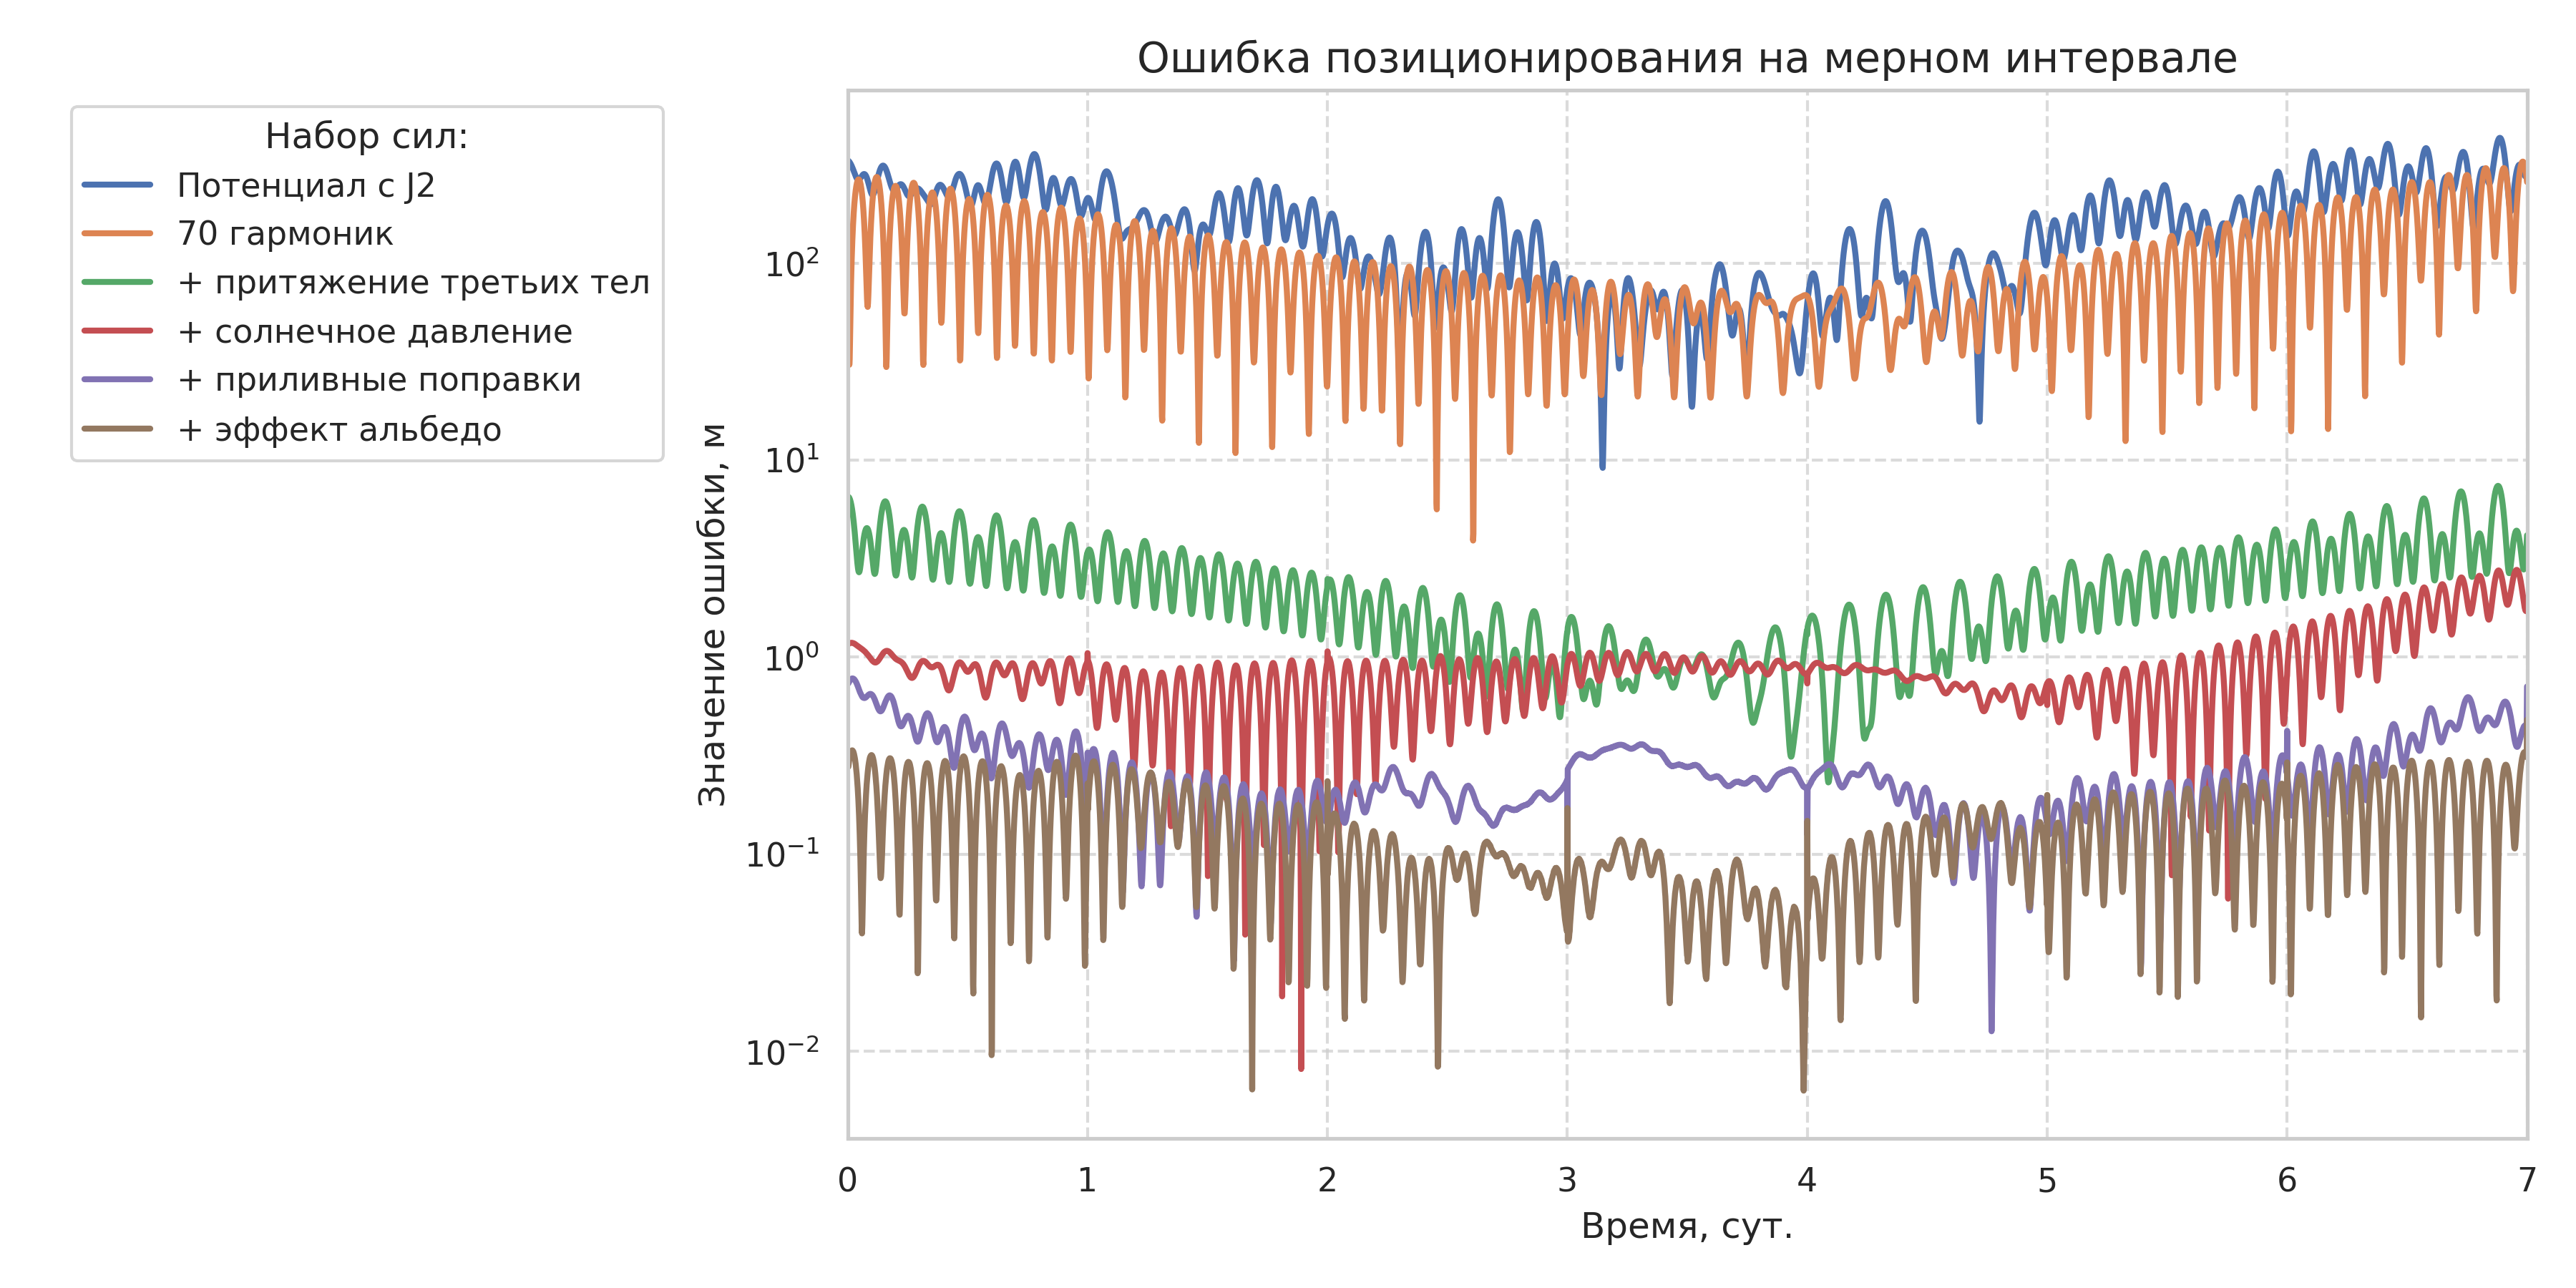
\includegraphics[width=\linewidth]{../images/solution/lageos/step_by_step.png}
    \captionof{figure}{График невязок на мерном интервале при использовании различных наборов сил
    и псевдоимпульсами}
    \label{fig:step_by_step}
 \end{figure}

Из результатов следует, что основные возмущающие факторы -- это нецентральность поля Земли,
притяжение третьих тел и солнечное давление. Учет этих сил позволяет получить среднюю
ошибку на мерном интервале меньше метра. Вклад приливных поправок и эффекта альбедо
значительно меньше. Таким образом, полная модель сил без параметризации дает среднюю ошибку
13 см.

Получить дециметровую точность помогает использвоние псевдоускорений. Данный подход
существенно уменьшает максимальную ошибку и сводит среднюю невзяку и стандартное отклонение
 к 10 и 11 сантиметрам соответственно. Для восстановления орбиты с субдециметровой точностью
 можно повышать количество псевдоускорений или добавить псевдоимпульсы. С комбинацией
 из 7 ускорений и 7 псевдоимпульсов средняя ошибка на мерном интервале падает до 5 см. 
 Такое значение ошибок близко к разнице между двумя агентствами, поэтому
 уточнение орбиты можно считать успешным.

Графики невязок на мерном интервале показаны на рис. \ref{fig:no_imp_no_acc}, 
\ref{fig:no_imp_with_acc}, \ref{fig:with_imp_with_acc}.

\begin{figure}[h!]
   \centering
   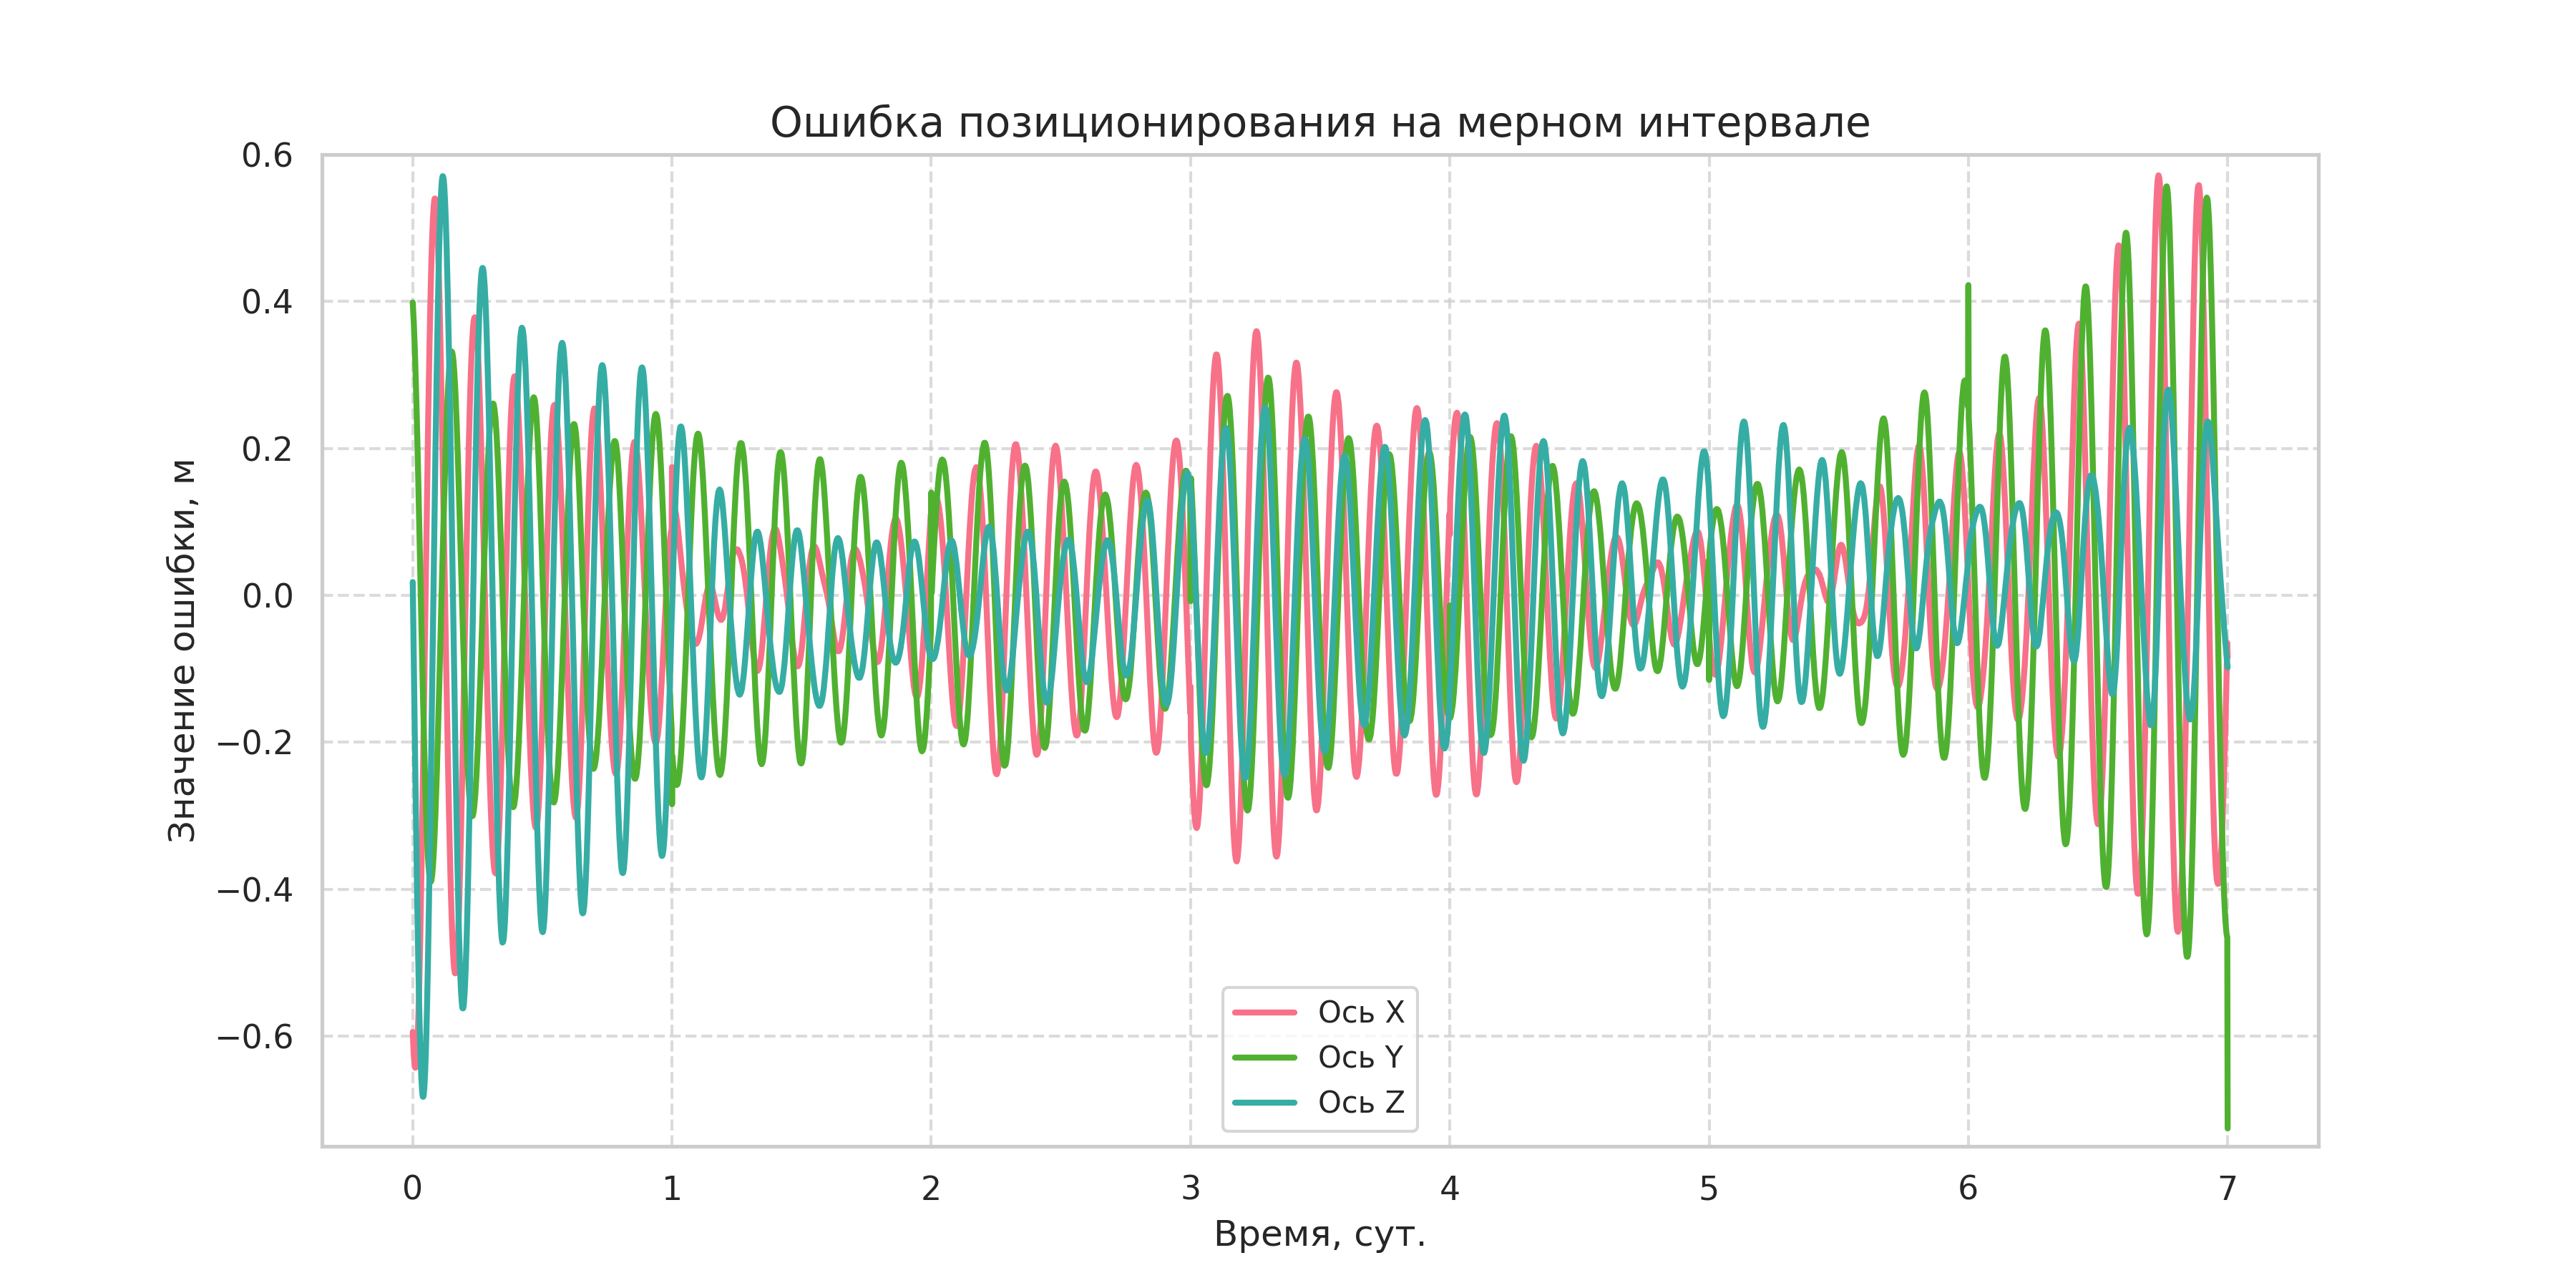
\includegraphics[width=\linewidth]{../images/solution/lageos/no_imp_no_acc.png}
   \captionof{figure}{График невязок на мерном интервале при использовании модели сил без параметризации}
   \label{fig:no_imp_no_acc}
\end{figure}

\begin{figure}[h!]
   \centering
   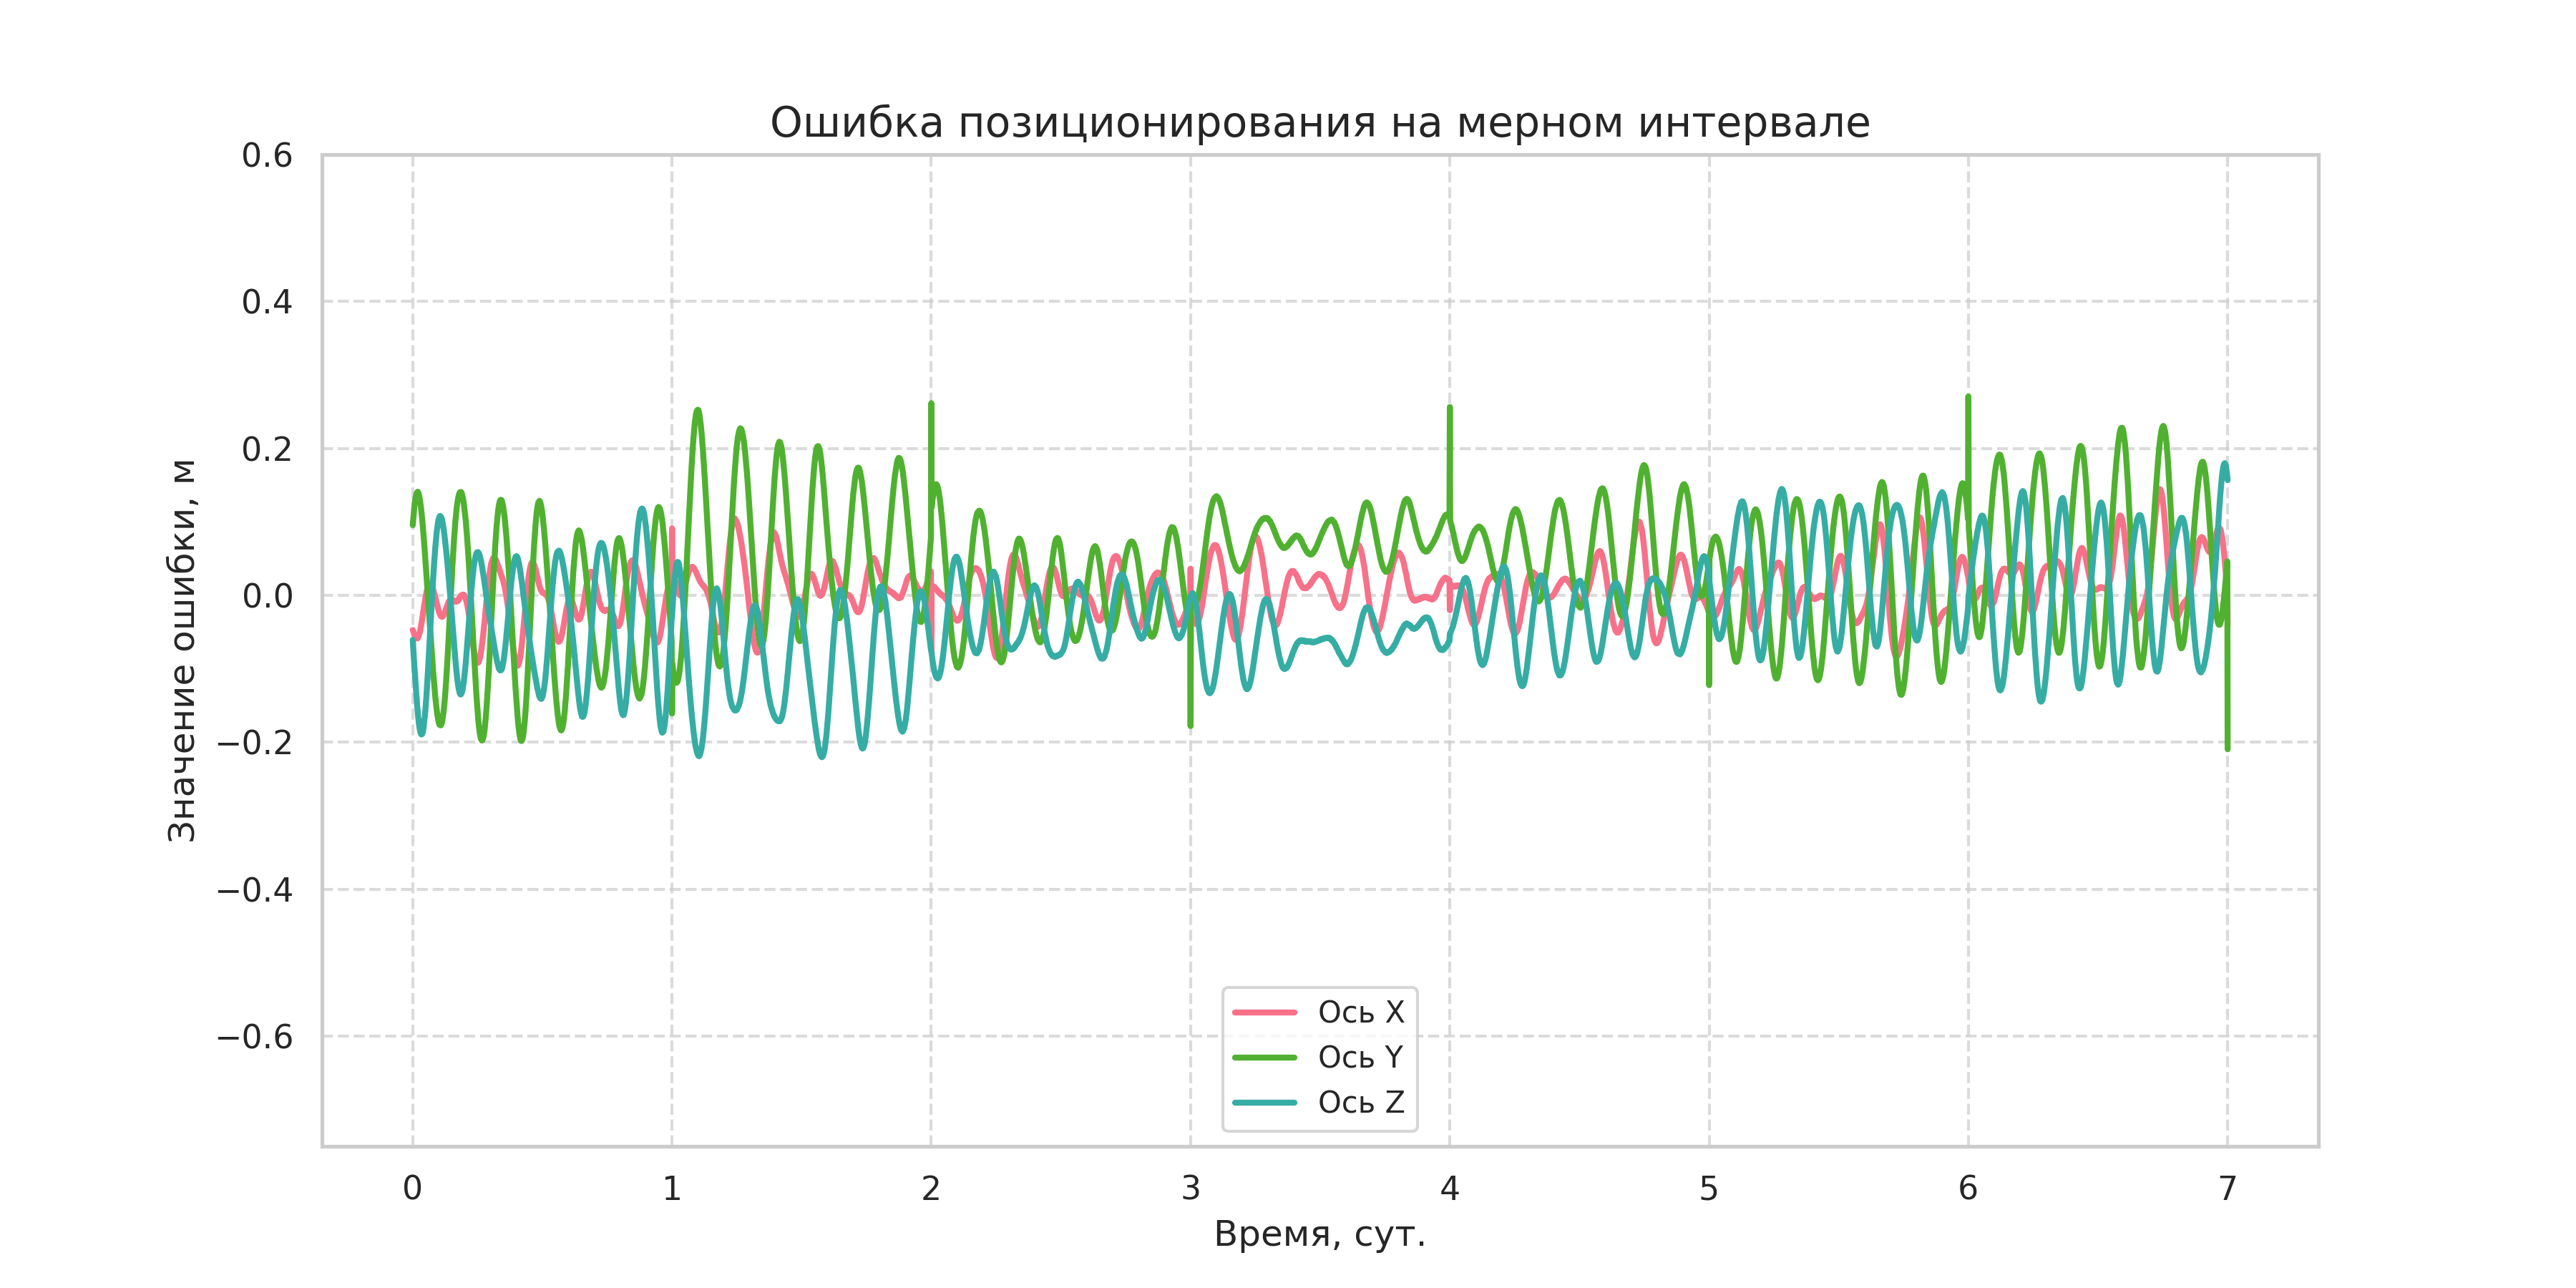
\includegraphics[width=\linewidth]{../images/solution/lageos/no_imp_with_acc.png}
   \captionof{figure}{График невязок на мерном интервале при использовании модели сил c псевдоускорениями}
   \label{fig:no_imp_with_acc}
\end{figure}

\begin{figure}[h!]
   \centering
   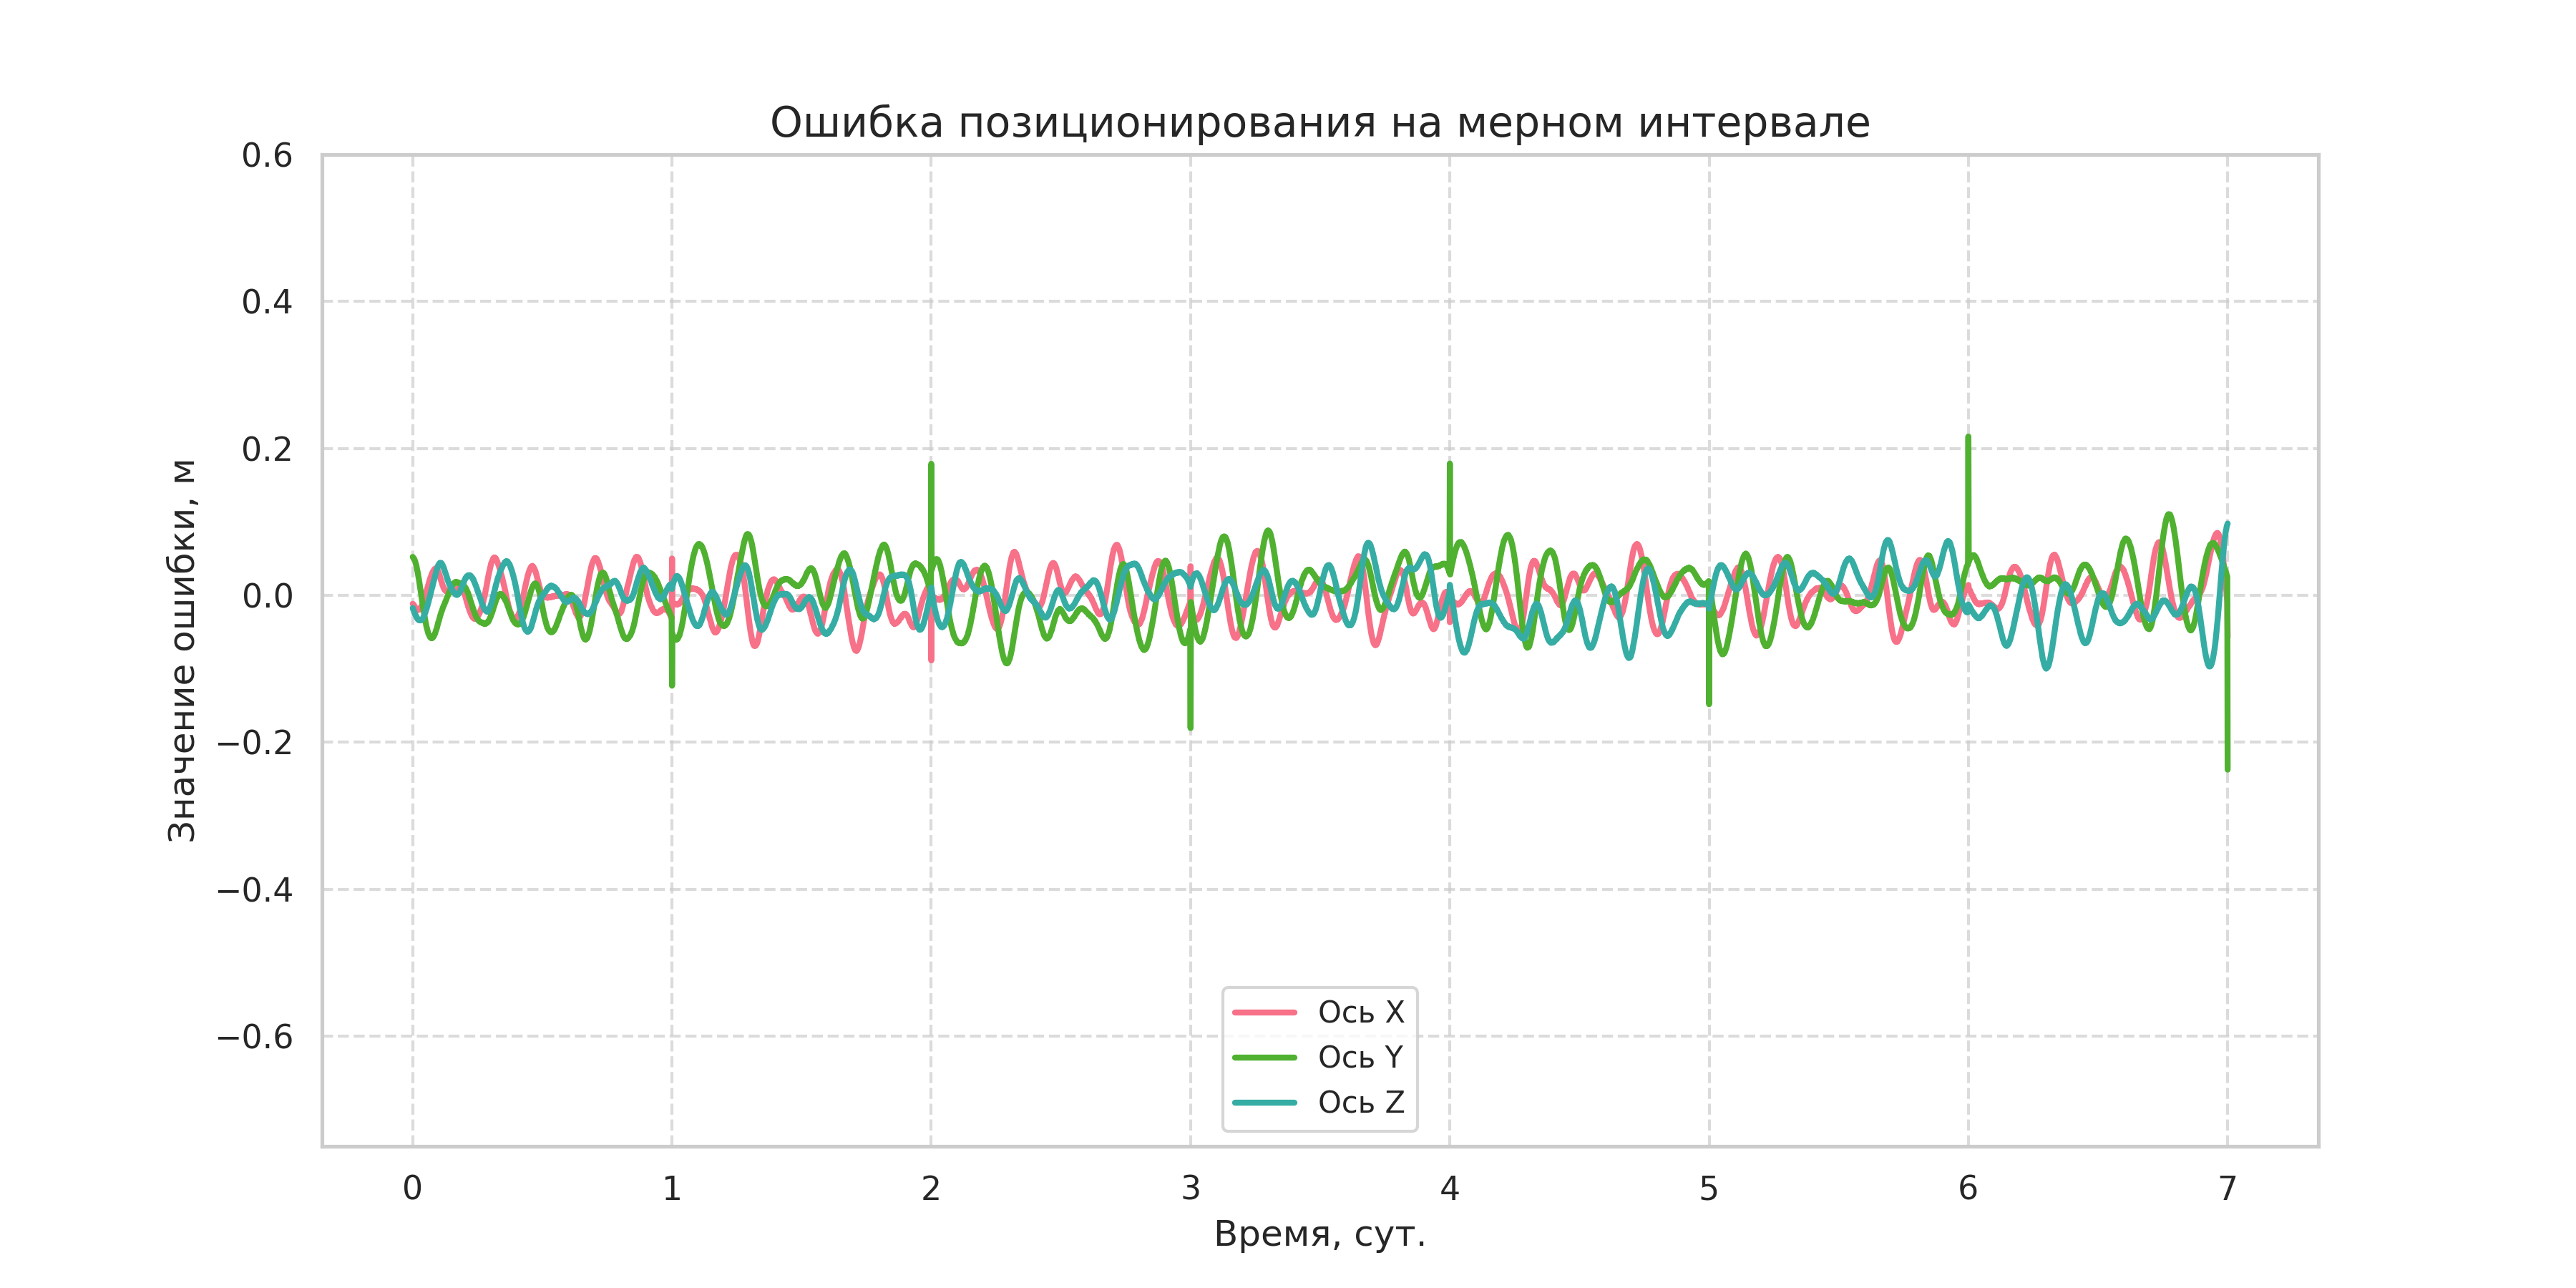
\includegraphics[width=\linewidth]{../images/solution/lageos/with_imp_with_acc.png}
   \captionof{figure}{График невязок на мерном интервале при использовании модели сил с псевдоускорениями
   и псевдоимпульсами}
   \label{fig:with_imp_with_acc}
\end{figure}

На рис. \ref{fig:no_imp_no_acc} хорошо видна специфика работы метода наименьших квадратов.
Метод оптимизрует решение таким образом, что в центральной области невязка получается
минимальной, а по краям симметрично растет. Это свидетельствует о правильной работе
алгоритма восстановления орбиты.

Валидация пройдена.

\input{parts/validation/cryosat.tex}

\newpage
    \section{Выводы}
\label{sec:Chapter5} \index{Chapter2}
В настоящей работе предложен метод ускорения расчета плотности атмосферы Земли с 
использованием четырехмерной интерполяции. 
Применение предложенного метода позволяет значительно повысить
быстродействие алгоритмов прогнозирования околоземных орбит.
Кроме того, реализована параметризация модели движения для прецизионного
восстановления орбиты. Проведена валидация разработанного программного комплекса на 
орбите космического аппарата LAGEOS-2.

В качестве дальнейшего направления работы можно выделить совершенствование метода
поиска рациональных параметров интерполянта, обеспечивающих приемлемую точность прогноза
при минимальных затратах памяти.
\newpage

    %% НЕ ТРОГАЙТЕ!!!
    \nocite{*}
    \bibliography{references}

    %% в зависимости от надобности подключаем раздел "Приложение"
    % \newpage
    % \input{Appendix.tex}
\end{document}
